\documentclass[12pt]{article}
\usepackage[utf8]{inputenc}
\usepackage[T1]{fontenc}
\usepackage[spanish,es-noshorthands]{babel}
\usepackage{geometry}
\usepackage{graphicx}
\usepackage{xcolor}
\usepackage[pdfauthor={Jorge Giovanni Correa Mejía},
            pdftitle={Anexo Fotográfico -- Rehabilitación de Tres Áreas Húmedas}]{hyperref}
\usepackage{titlesec}
\usepackage{fancyhdr}
\usepackage{caption}
\usepackage{parskip}
\usepackage[osf]{mathpazo}
\usepackage{eulervm}
\usepackage{microtype}
\usepackage{float}
\usepackage{enumitem}
\geometry{letterpaper, margin=1.5cm, top=2cm, bottom=2cm}
\clubpenalty=10000
\widowpenalty=10000
\definecolor{primary}{RGB}{25, 55, 109}
\definecolor{secondary}{RGB}{0, 105, 148}
\hypersetup{colorlinks=true, linkcolor=primary, urlcolor=secondary}
\setcounter{secnumdepth}{3}
\titleformat{\section}{\Large\bfseries\color{primary}\lsstyle}{\thesection.}{0.6em}{}[{\vspace{-0.2em}\rule{\textwidth}{0.5pt}}]
\pagestyle{fancy}
\fancyhf{}
\fancyhead[L]{\footnotesize\textcolor{primary!60!black}{Anexo Fotográfico -- Rehabilitación de Tres Áreas Húmedas}}
\fancyhead[R]{\footnotesize\textcolor{primary!60!black}{Junio 2026}}
\fancyfoot[C]{\thepage}
\setlength{\headheight}{12.7pt}
\renewcommand{\headrulewidth}{0.4pt}
\renewcommand{\footrulewidth}{0pt}
\captionsetup[figure]{font=small,skip=4pt,labelfont={bf,color=primary},textfont={color=primary!80!black},labelsep=space}
\begin{document}
\thispagestyle{empty}
\begin{titlepage}
  \centering
  \vspace*{1.5cm}
  {\color{primary}\rule{\textwidth}{2.5pt}}\\[1cm]
  {\Huge\bfseries\color{primary}\lsstyle ANEXO 6}\\[1.2cm]
  {\LARGE\bfseries\color{secondary} Registro Fotográfico}\\[0.6cm]
  {\large\color{primary!70!black} Estado Actual de las Áreas Húmedas}\\[1.5cm]
  {\color{primary}\rule{\textwidth}{2.5pt}}\\[2cm]
  \begin{minipage}{0.8\textwidth}
    \centering\large
    \textbf{Proyecto:} Rehabilitación Integral de Tres Áreas Húmedas\\[0.3cm]
    \textbf{Propietario:} Francisco Javier Rondon Lagos\\[0.3cm]
    \textbf{Dirección:} Calle 78 B No. 120-49, Bloque 1, Apto 401\\[0.3cm]
    \textbf{Barrio:} Reserva de Granada 3, Bogotá\\[0.3cm]
    \textbf{Fecha del registro:} 9 de noviembre de 2025
  \end{minipage}
  \vfill
  {\small\color{primary!60!black} Documento técnico -- Registro fotográfico del estado anterior a la intervención}
  \vspace{1cm}
  \begin{center}
    \rule{8cm}{0.5pt}\\[0.3cm]
    {\bfseries Ing. Jorge Giovanni Correa Mejía}\\[0.1cm]
    CC 4.252.533\\[0.1cm]
    Director de Proyecto
  \end{center}
\end{titlepage}
\newpage
\section*{\color{primary}\lsstyle Índice de Figuras}
\addcontentsline{toc}{section}{Índice de figuras}
\listoffigures
\newpage
\section{Baño 1}
\noindent\textbf{Estado general:} REGULAR.
\medskip
\noindent\textbf{Patologías identificadas:}
\begin{itemize}[leftmargin=*,nosep]
  \item \textbf{Humedad ascendente} en muros perimetrales — se observa desprendimiento generalizado de pañete en la zona del zócalo, con eflorescencia salina blanquecina en los primeros 30 cm del muro sur.
  \item \textbf{Fisuración múltiple} en enchape cerámico de muros — grietas capilares de hasta 15 cm de longitud en paños nororiental y suroccidental, compatibles con movimientos diferenciales de la estructura.
  \item \textbf{Desprendimiento de boquillas} en un 40\% del área enchapada — pérdida de adherencia del mortero de junta, con riesgo de filtración hacia el trasdosado.
  \item \textbf{Deterioro de tubería de suministro de agua caliente} — yellowing y fragilización del PVC en tramos expuestos a radiación UV, con deformación en los acoples de la válvula de paso.
  \item \textbf{Deterioro de sellos perimetrales} en unión lavamanos-mesón y sanitario-piso, con presencia de hongos y acumulación de suciedad.
  \item \textbf{Perforaciones y remates provisionales} en muro norte, producto de instalaciones anteriores mal reparadas.
  \item \textbf{Descuadre de las divisiones de baño} — los tabiques divisorios no presentan alineación vertical con respecto al eje estructural, con desviaciones de hasta 2 cm en el paño noroccidental, evidenciando modificaciones no estructurales en la distribución original del espacio.
\end{itemize}
\medskip
\noindent\textbf{Zonas críticas:} Muro sur (humedad ascendente), perímetro del sanitario (sellos deteriorados), unión piso-pared en ducha (boquillas desprendidas), grifería de lavamanos (óxido), divisiones de baño (descuadre).
\bigskip
\begin{figure}[H]
\centering
\begin{tabular}{cc}
\parbox{0.45\textwidth}{\centering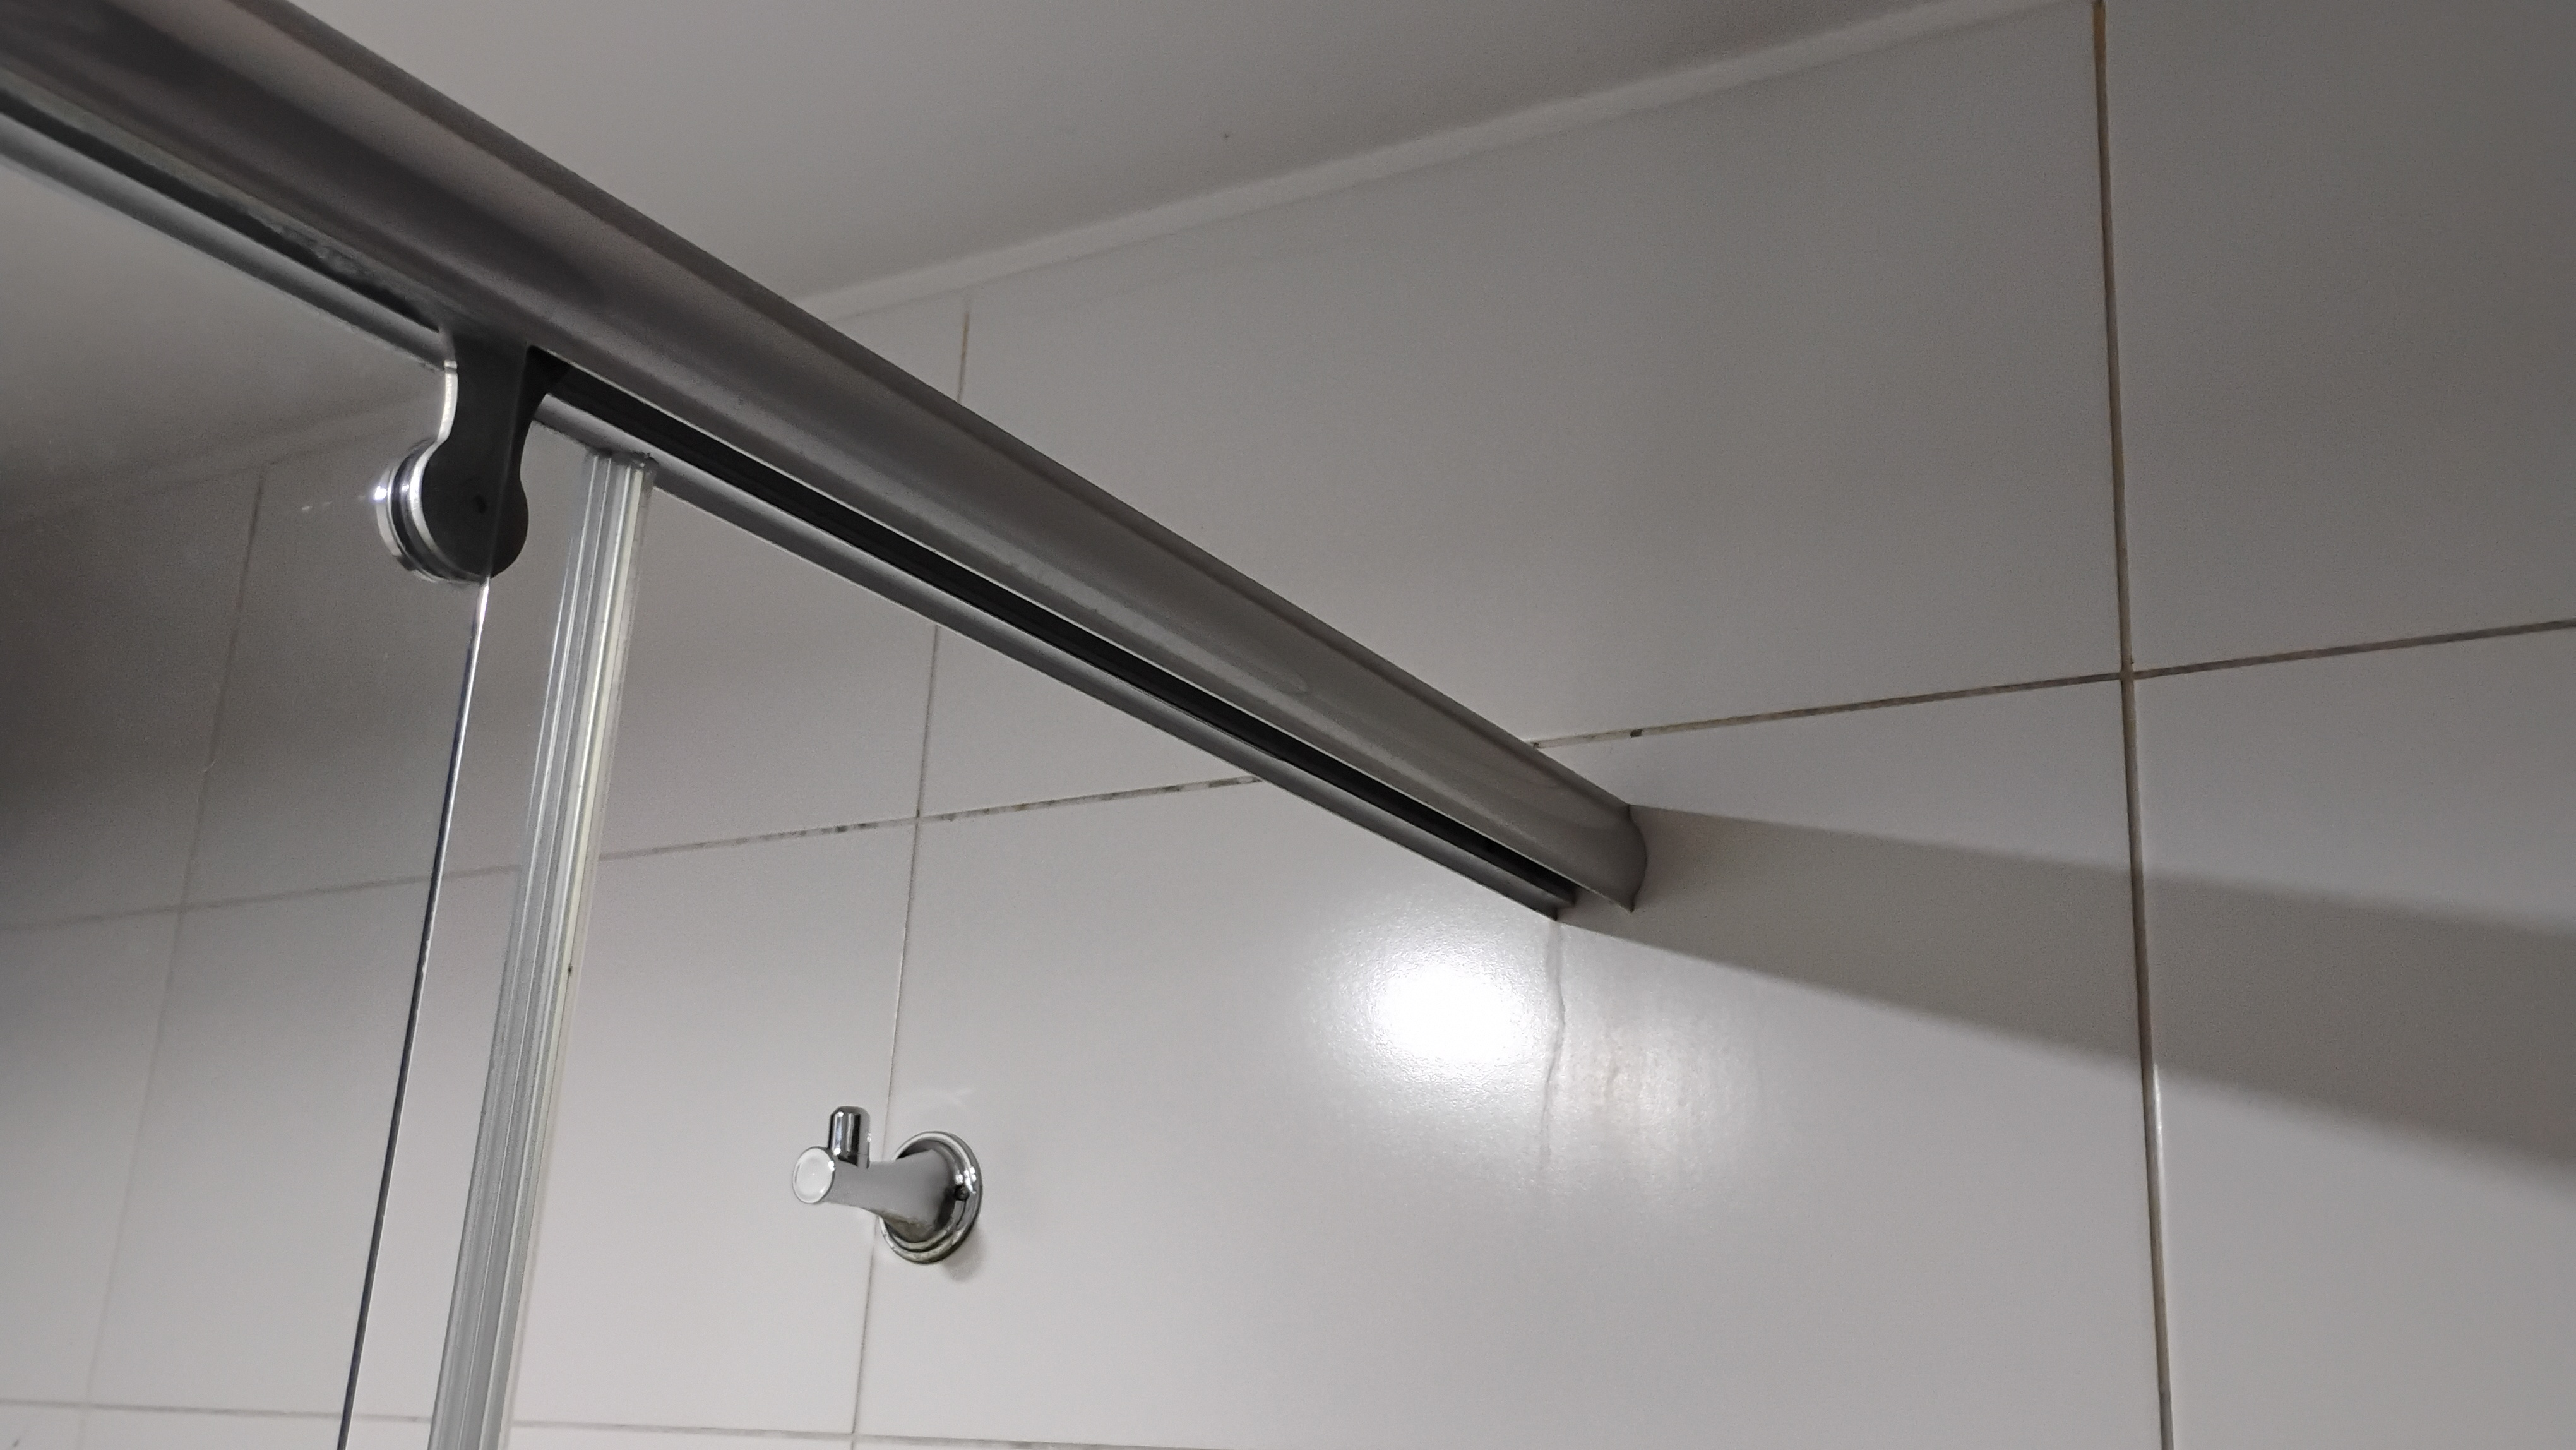
\includegraphics[width=\linewidth]{../img/IMG_20251109_150617307.jpg}\\[2pt]{\footnotesize\color{primary!60!black}Foto~1 -- 15:06:17}} & \parbox{0.45\textwidth}{\centering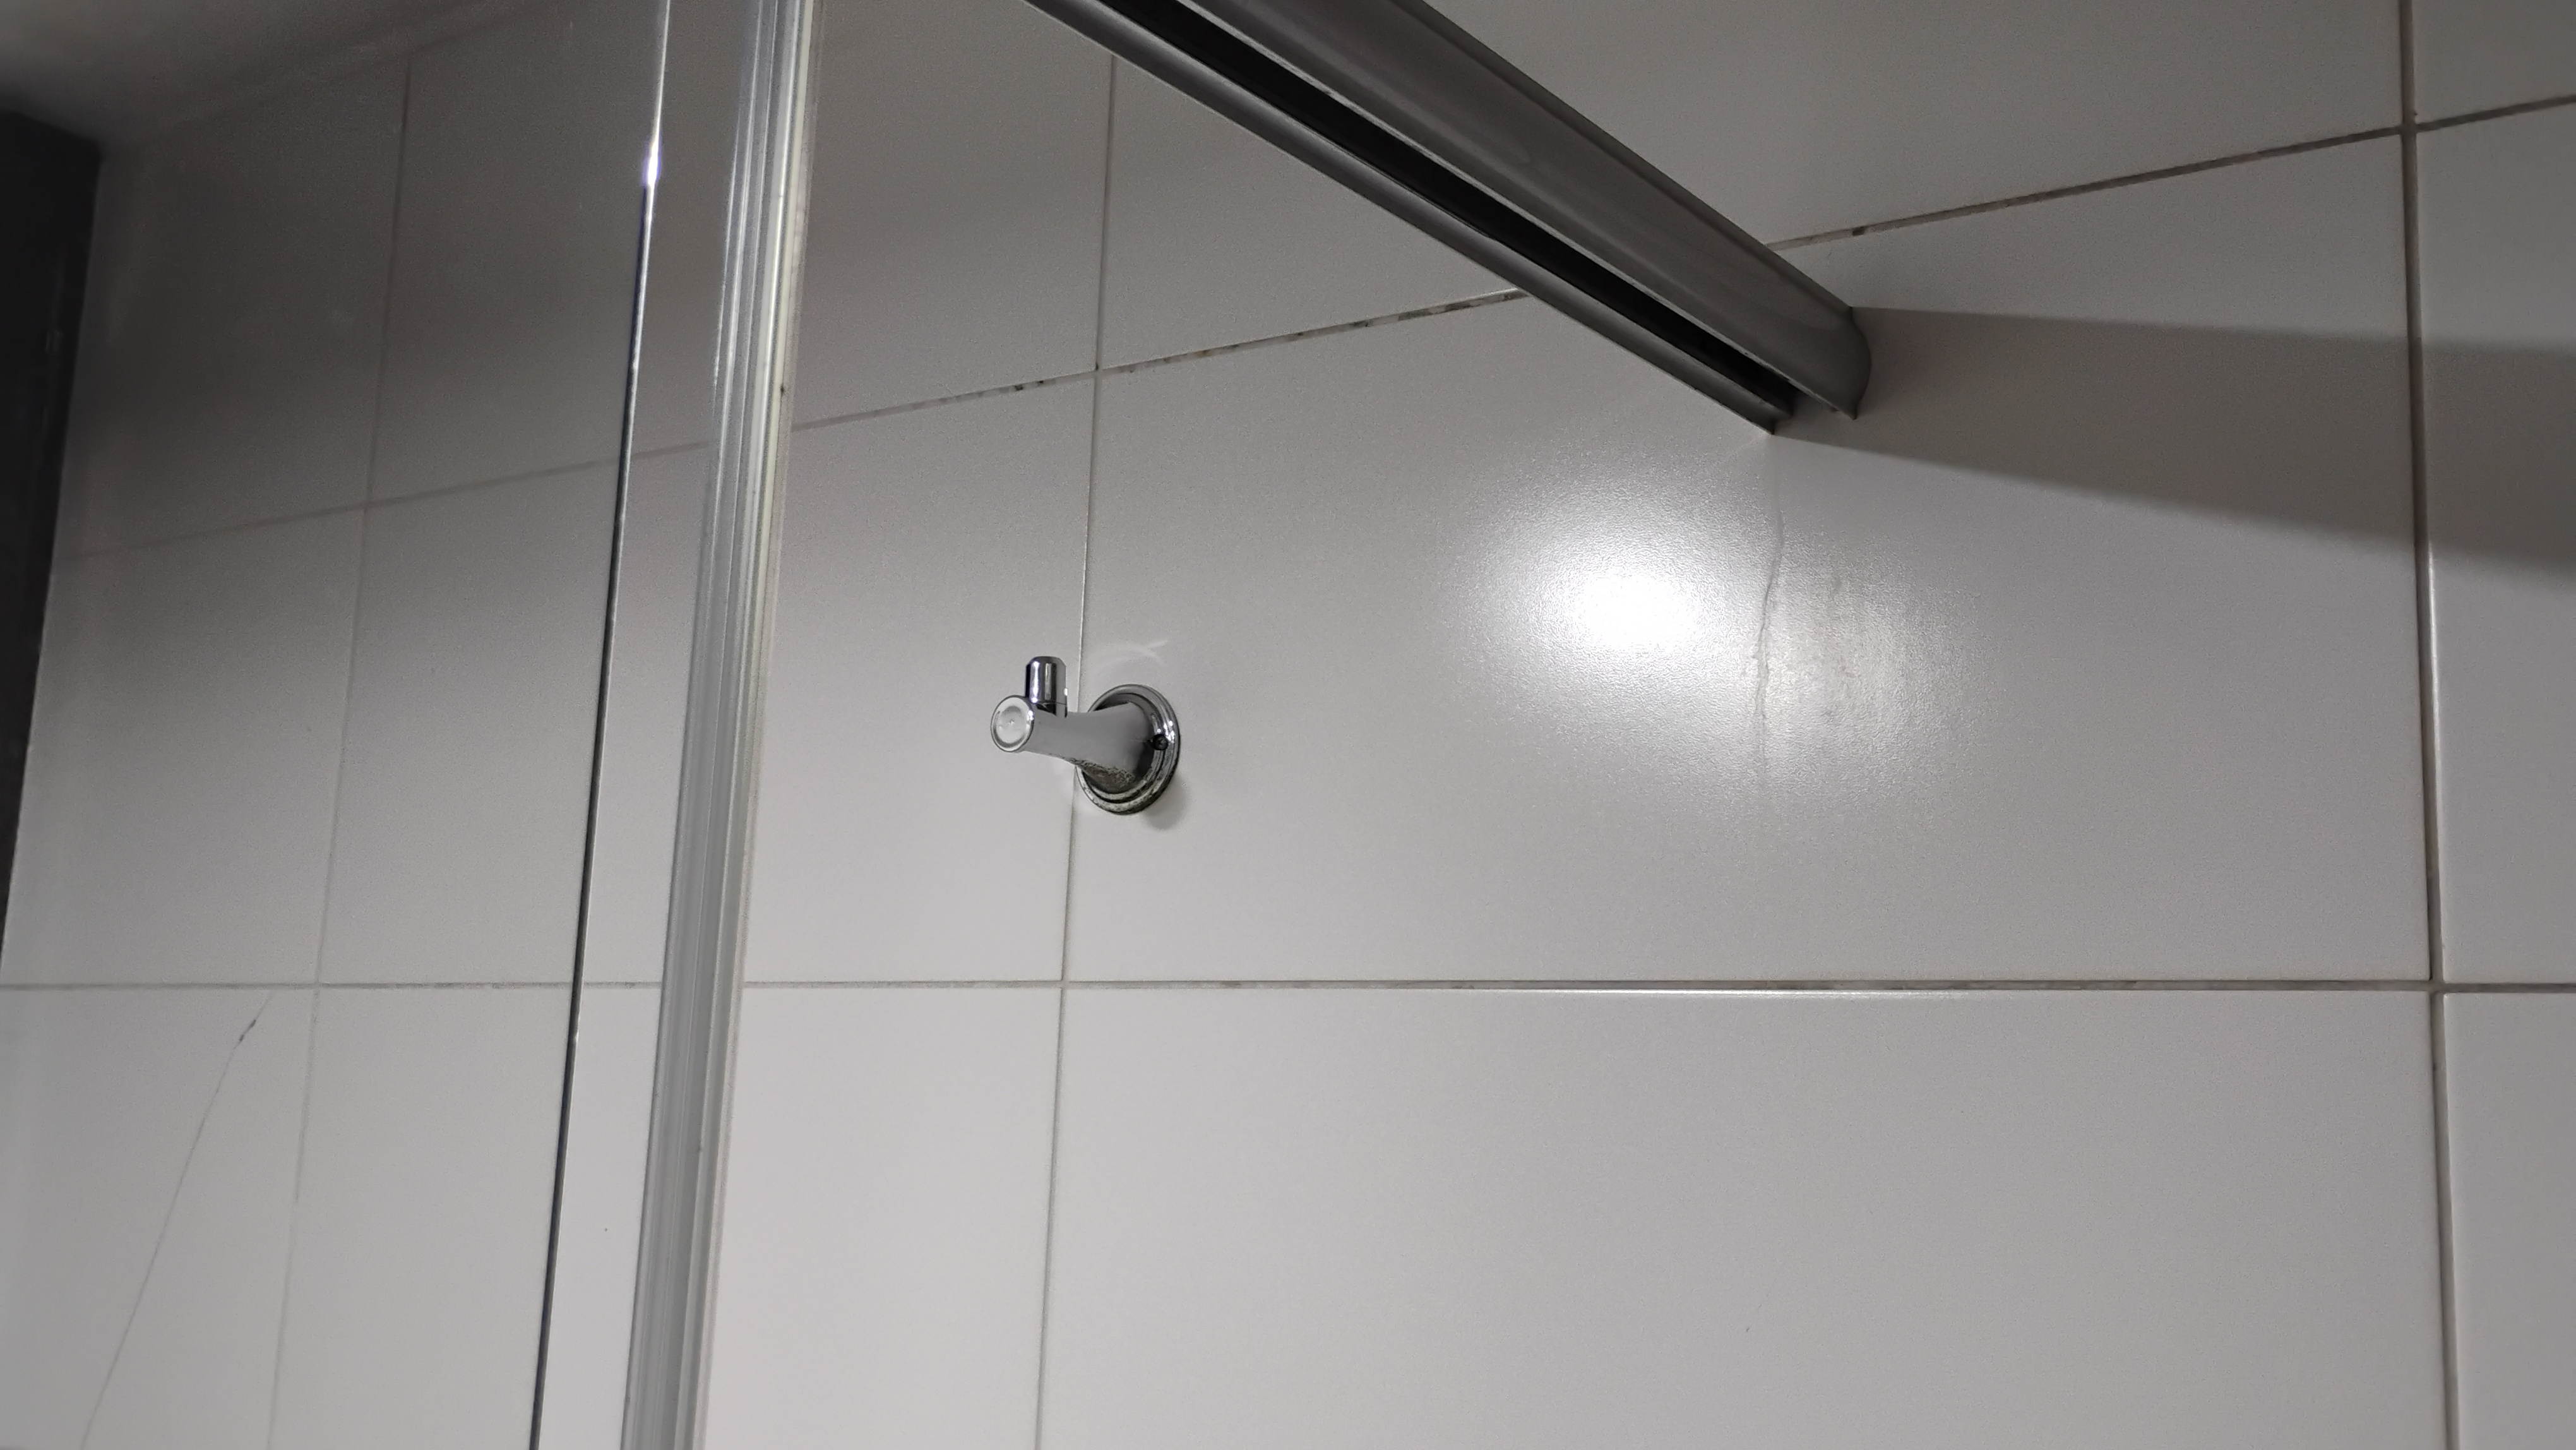
\includegraphics[width=\linewidth]{../img/IMG_20251109_150618891.jpg}\\[2pt]{\footnotesize\color{primary!60!black}Foto~2 -- 15:06:18}} \\[4pt]
\parbox{0.45\textwidth}{\centering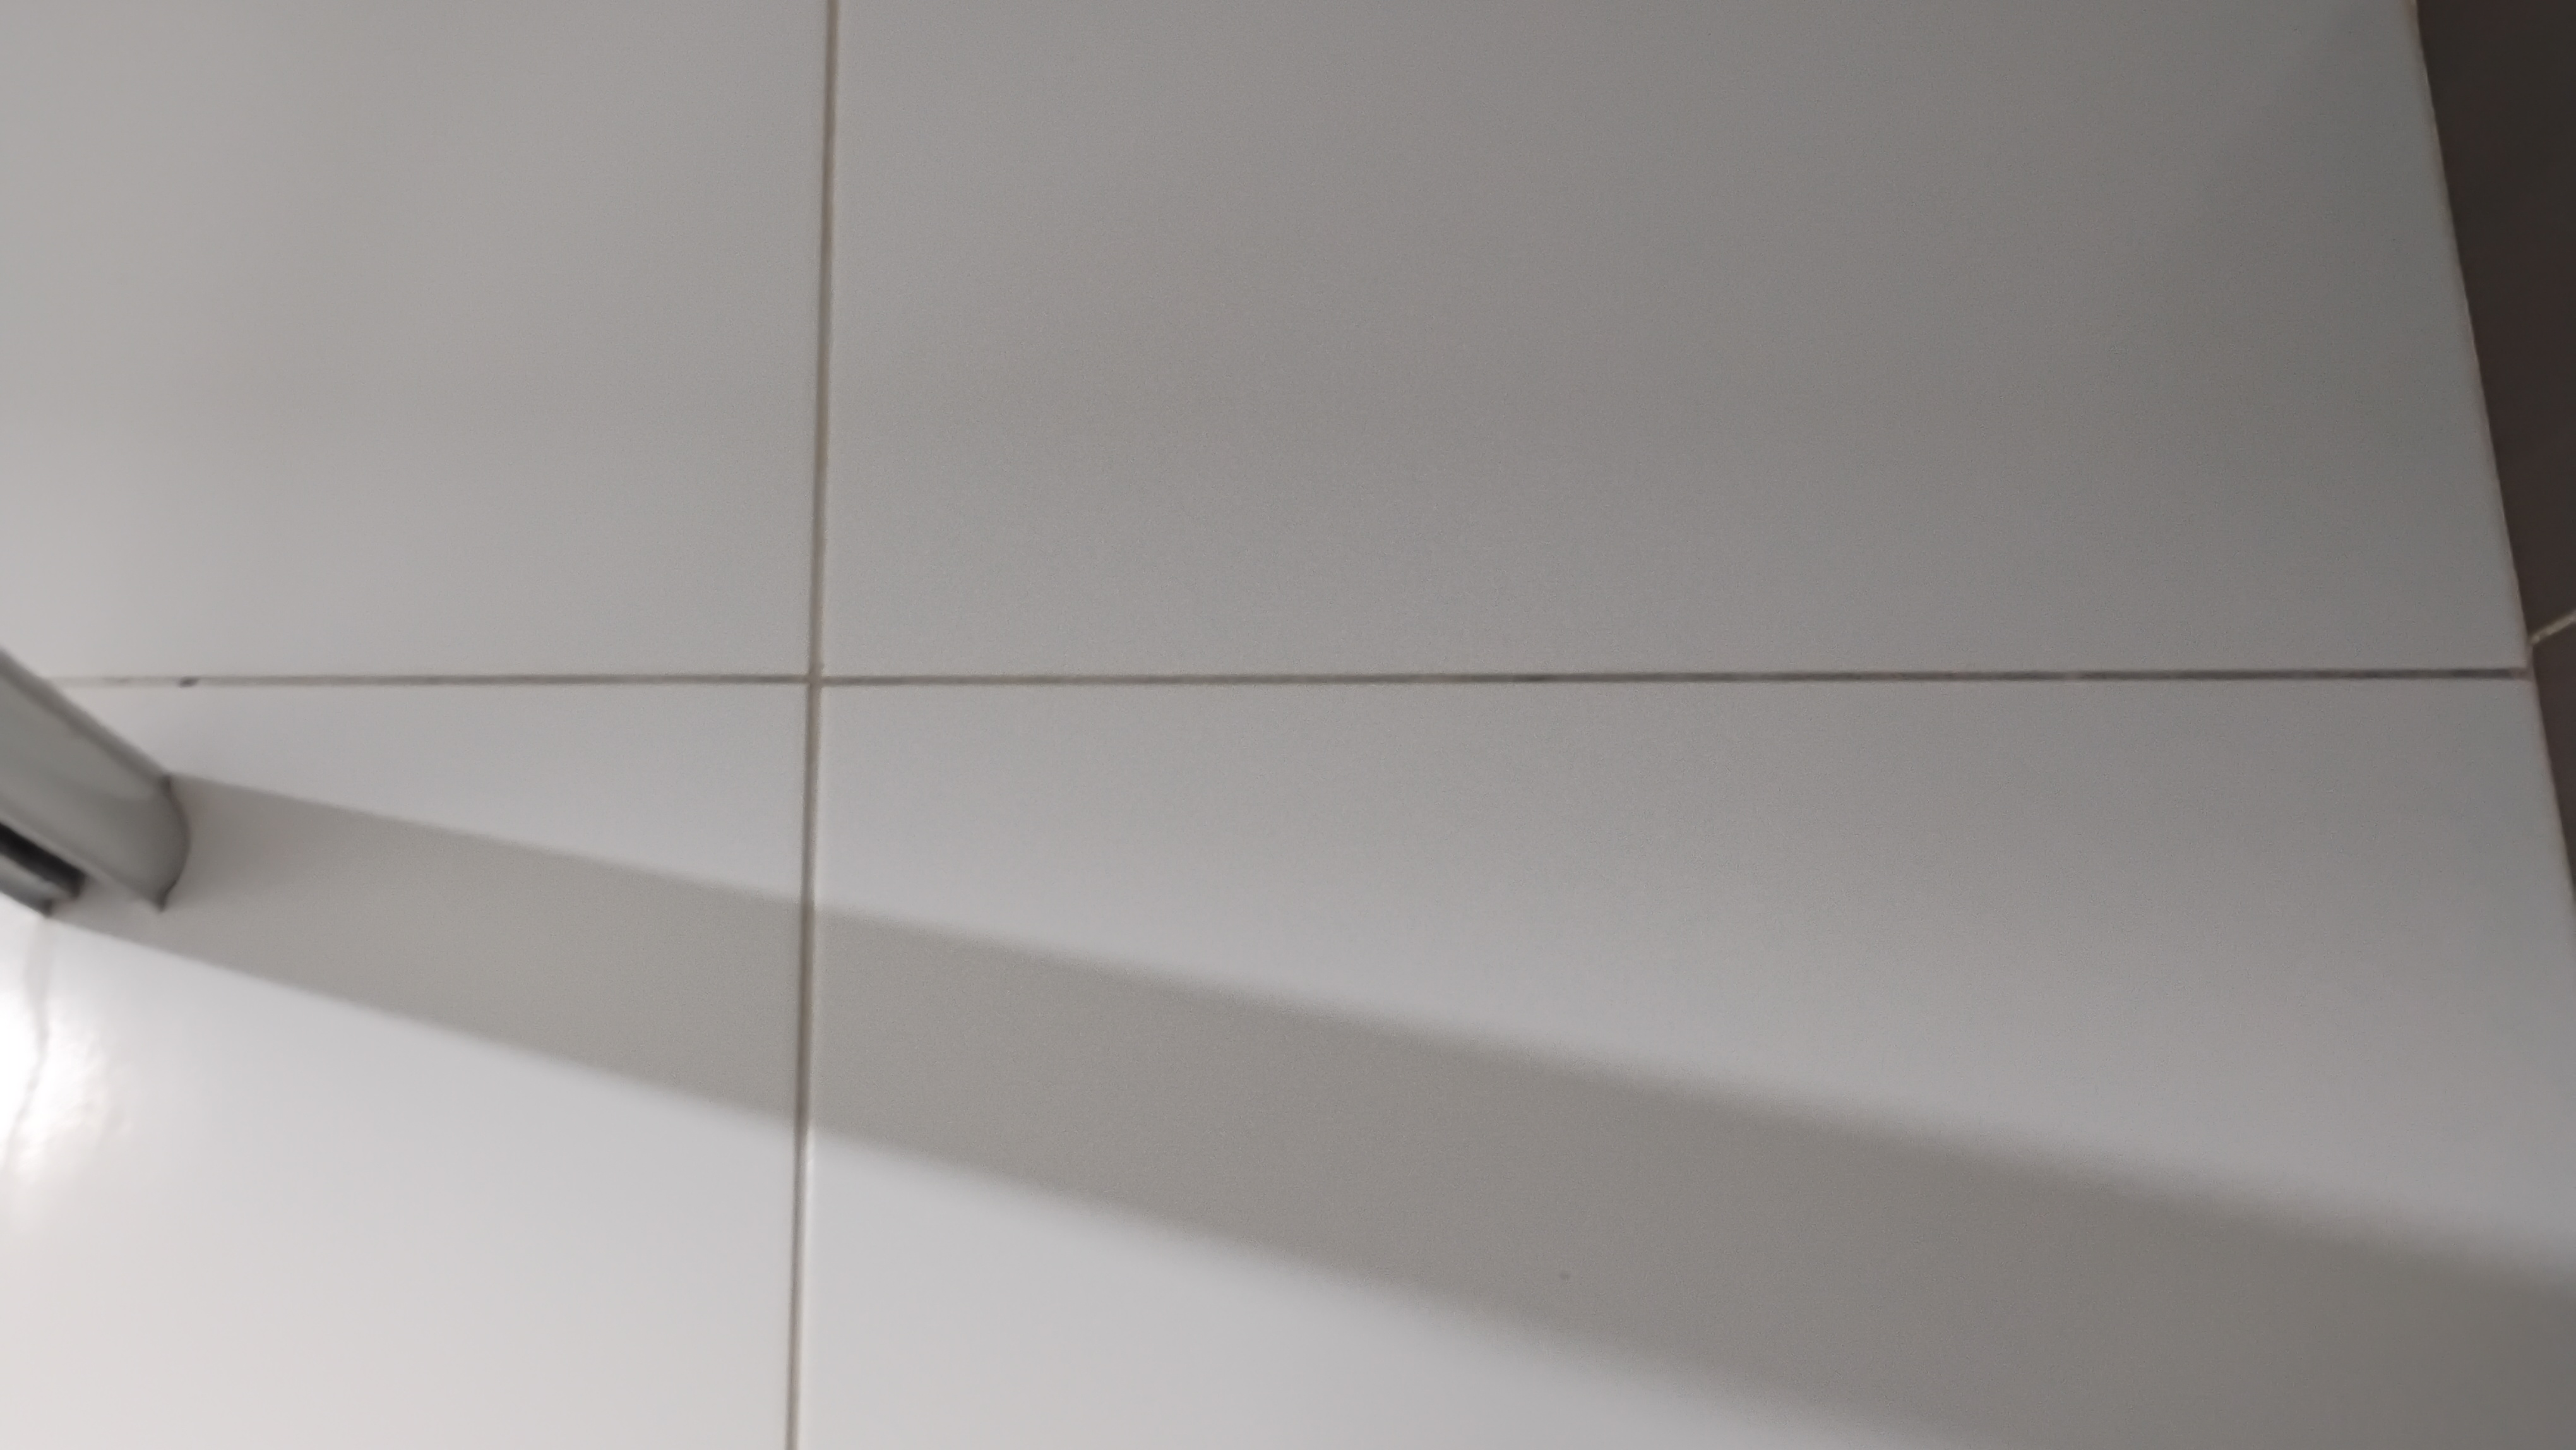
\includegraphics[width=\linewidth]{../img/IMG_20251109_150631285.jpg}\\[2pt]{\footnotesize\color{primary!60!black}Foto~3 -- 15:06:31}} & \parbox{0.45\textwidth}{\centering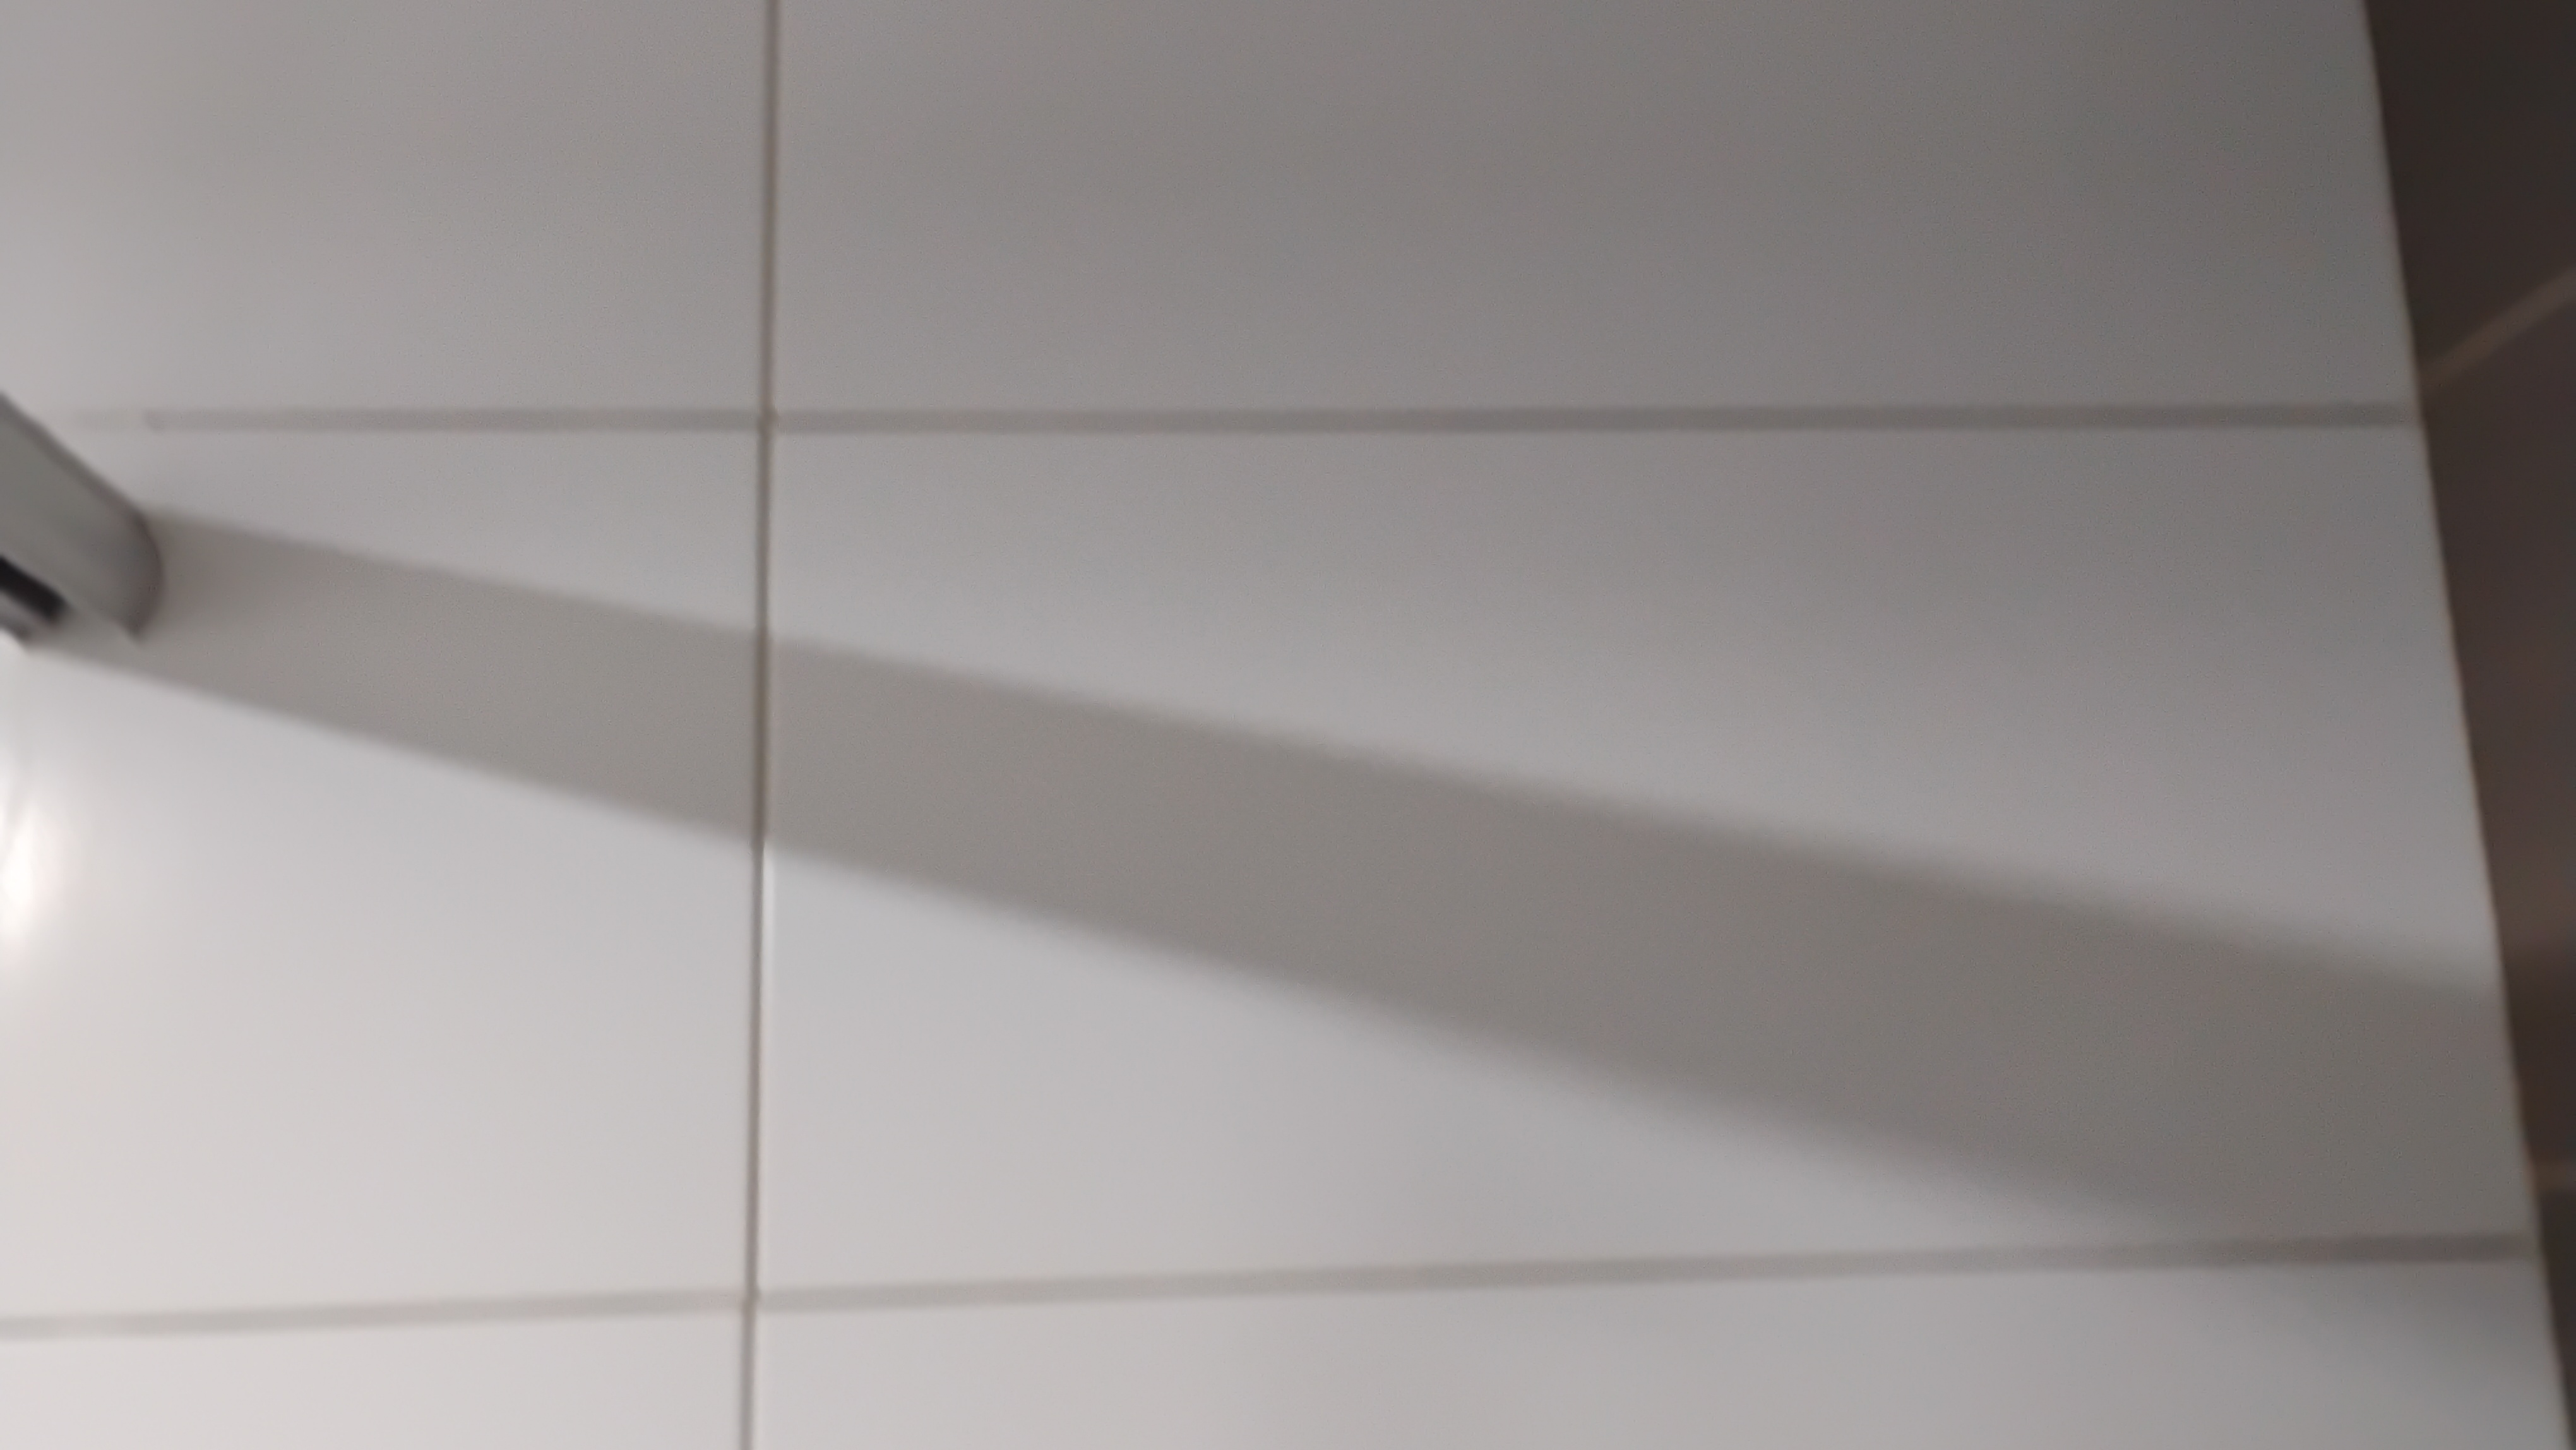
\includegraphics[width=\linewidth]{../img/IMG_20251109_150632163.jpg}\\[2pt]{\footnotesize\color{primary!60!black}Foto~4 -- 15:06:32}} \\[4pt]
\parbox{0.45\textwidth}{\centering
\includegraphics[width=\linewidth]{../img/IMG_20251109_150633149.jpg}\\[2pt]{\footnotesize\color{primary!60!black}Foto~5 -- 15:06:33}} & \parbox{0.45\textwidth}{\centering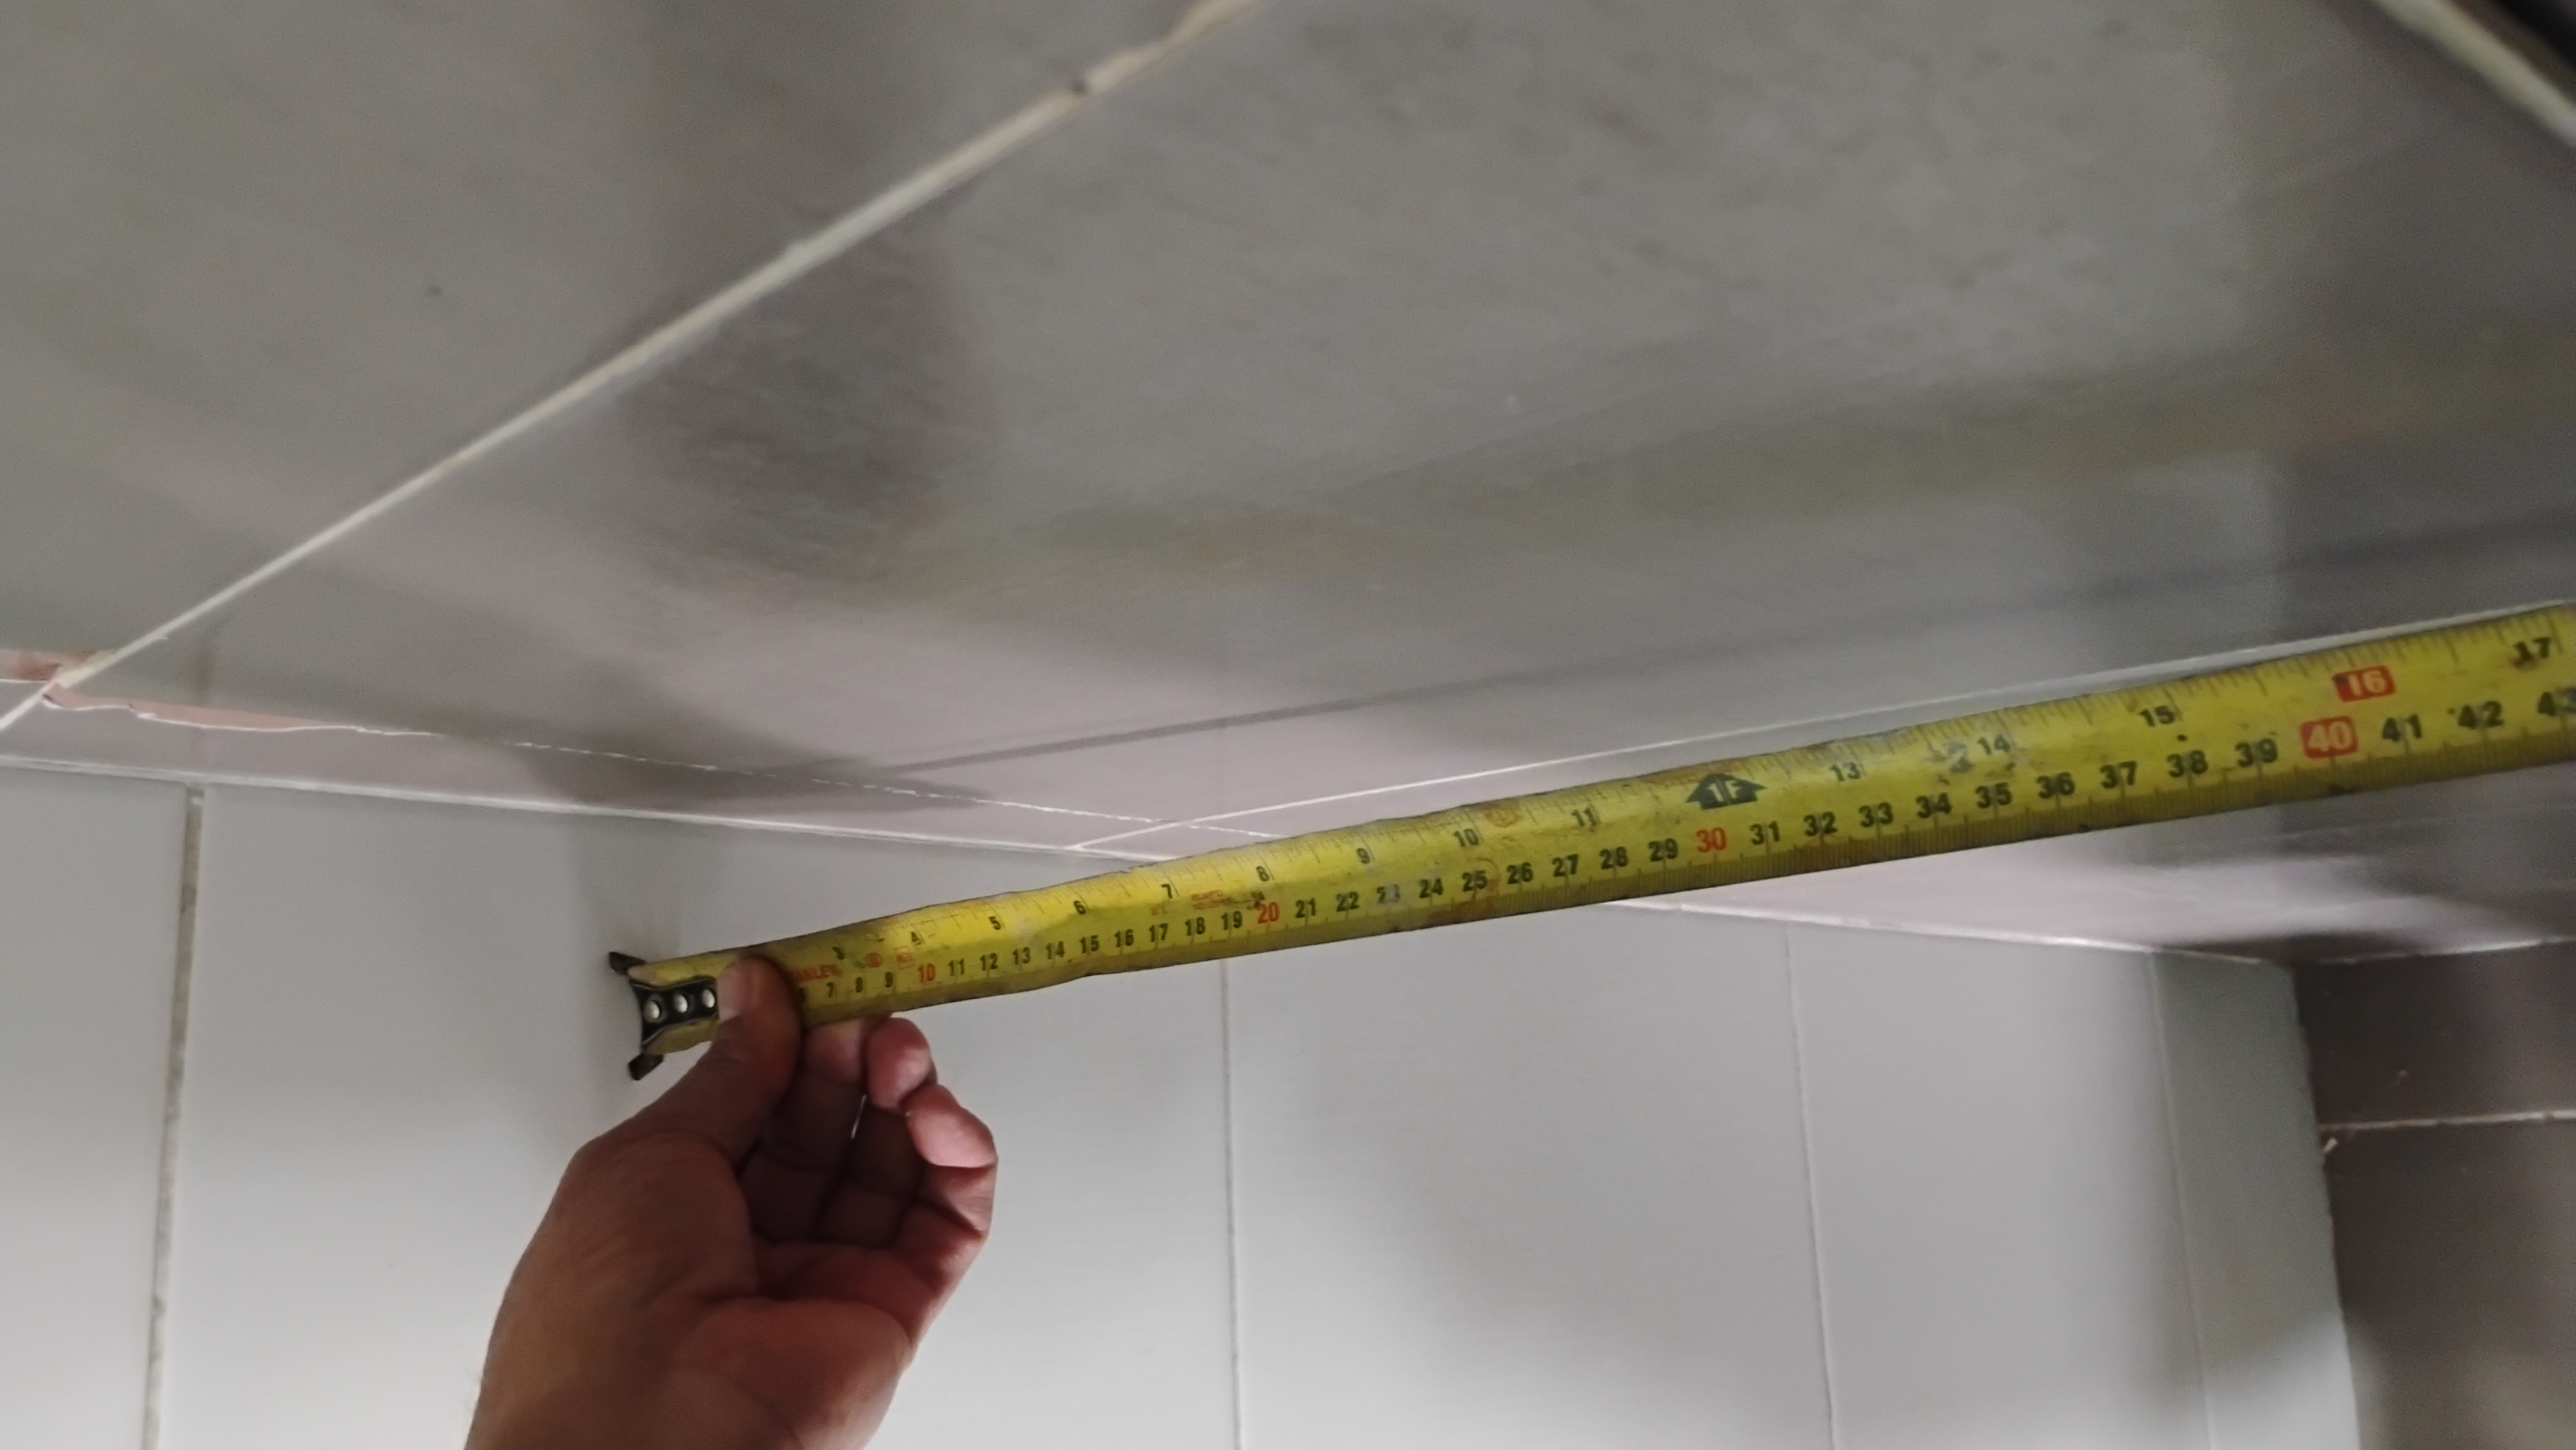
\includegraphics[width=\linewidth]{../img/IMG_20251109_150927279.jpg}\\[2pt]{\footnotesize\color{primary!60!black}Foto~6 -- 15:09:27}} \\[4pt]
\end{tabular}
\caption{División de Baño: Fotos 1 al 6.}\end{figure}
\newpage
\begin{figure}[H]
\centering
\begin{tabular}{cc}
\parbox{0.45\textwidth}{\centering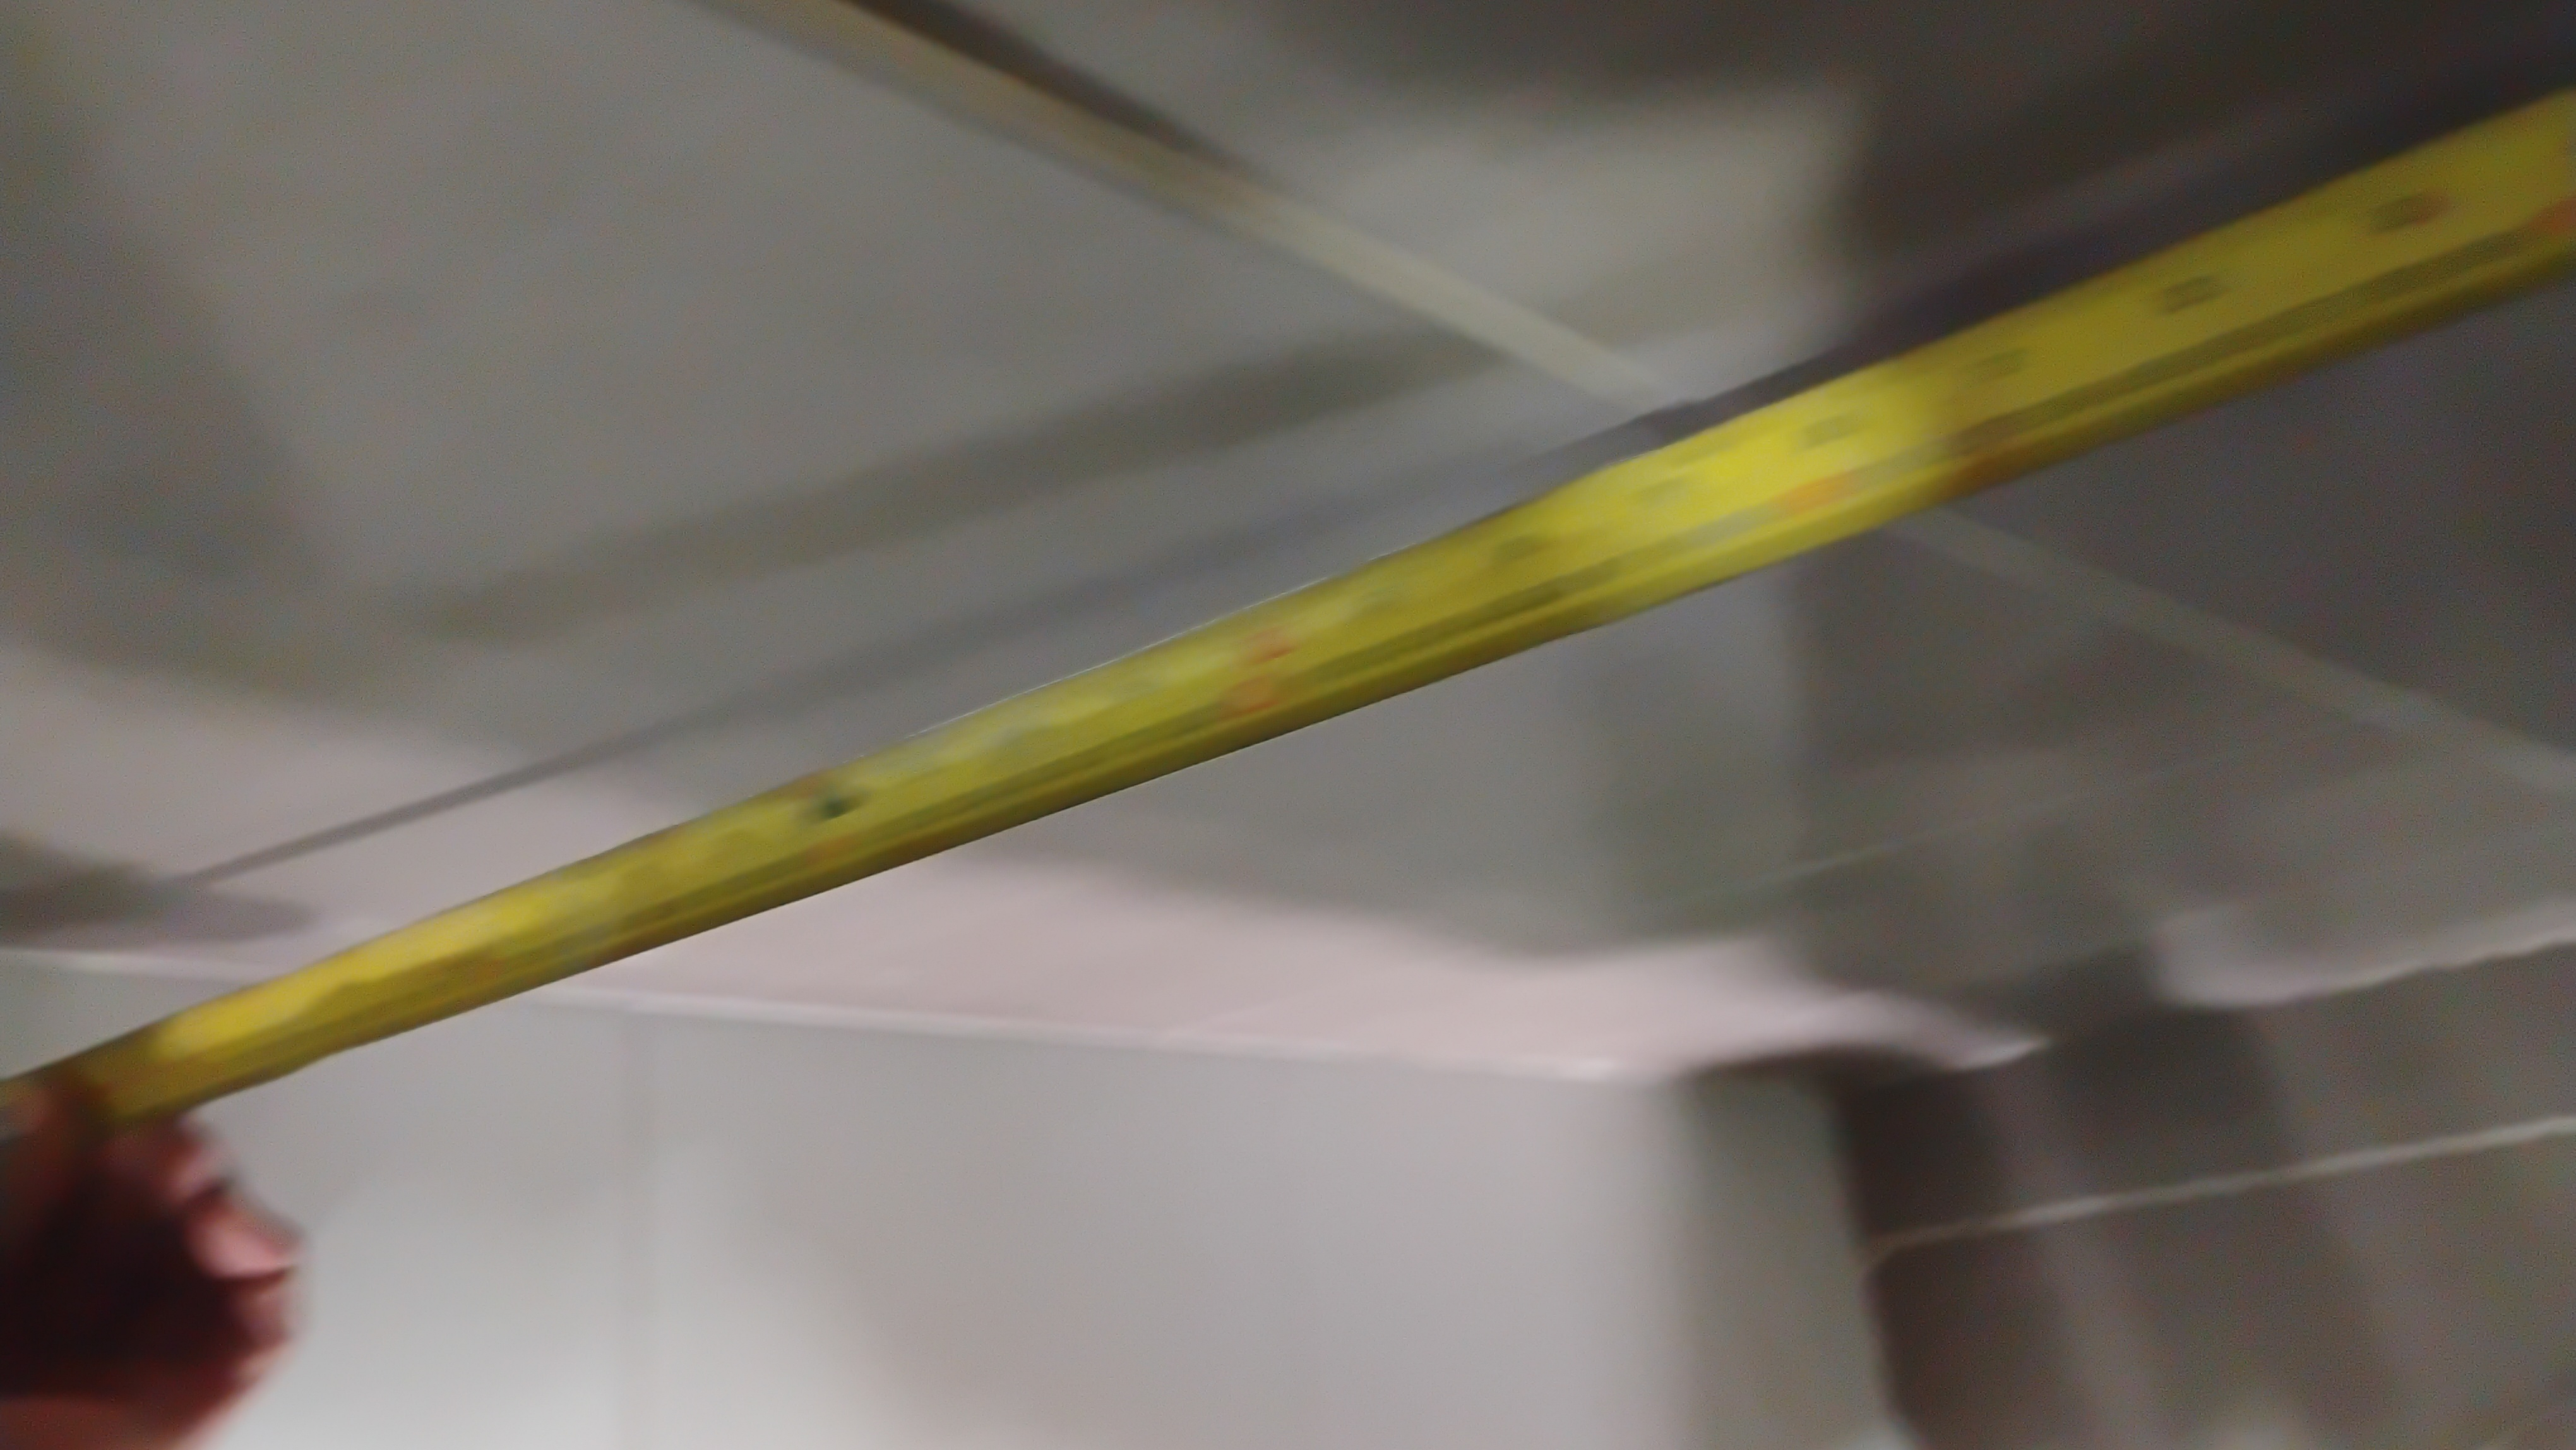
\includegraphics[width=\linewidth]{../img/IMG_20251109_150928983.jpg}\\[2pt]{\footnotesize\color{primary!60!black}Foto~7 -- 15:09:28}} & \parbox{0.45\textwidth}{\centering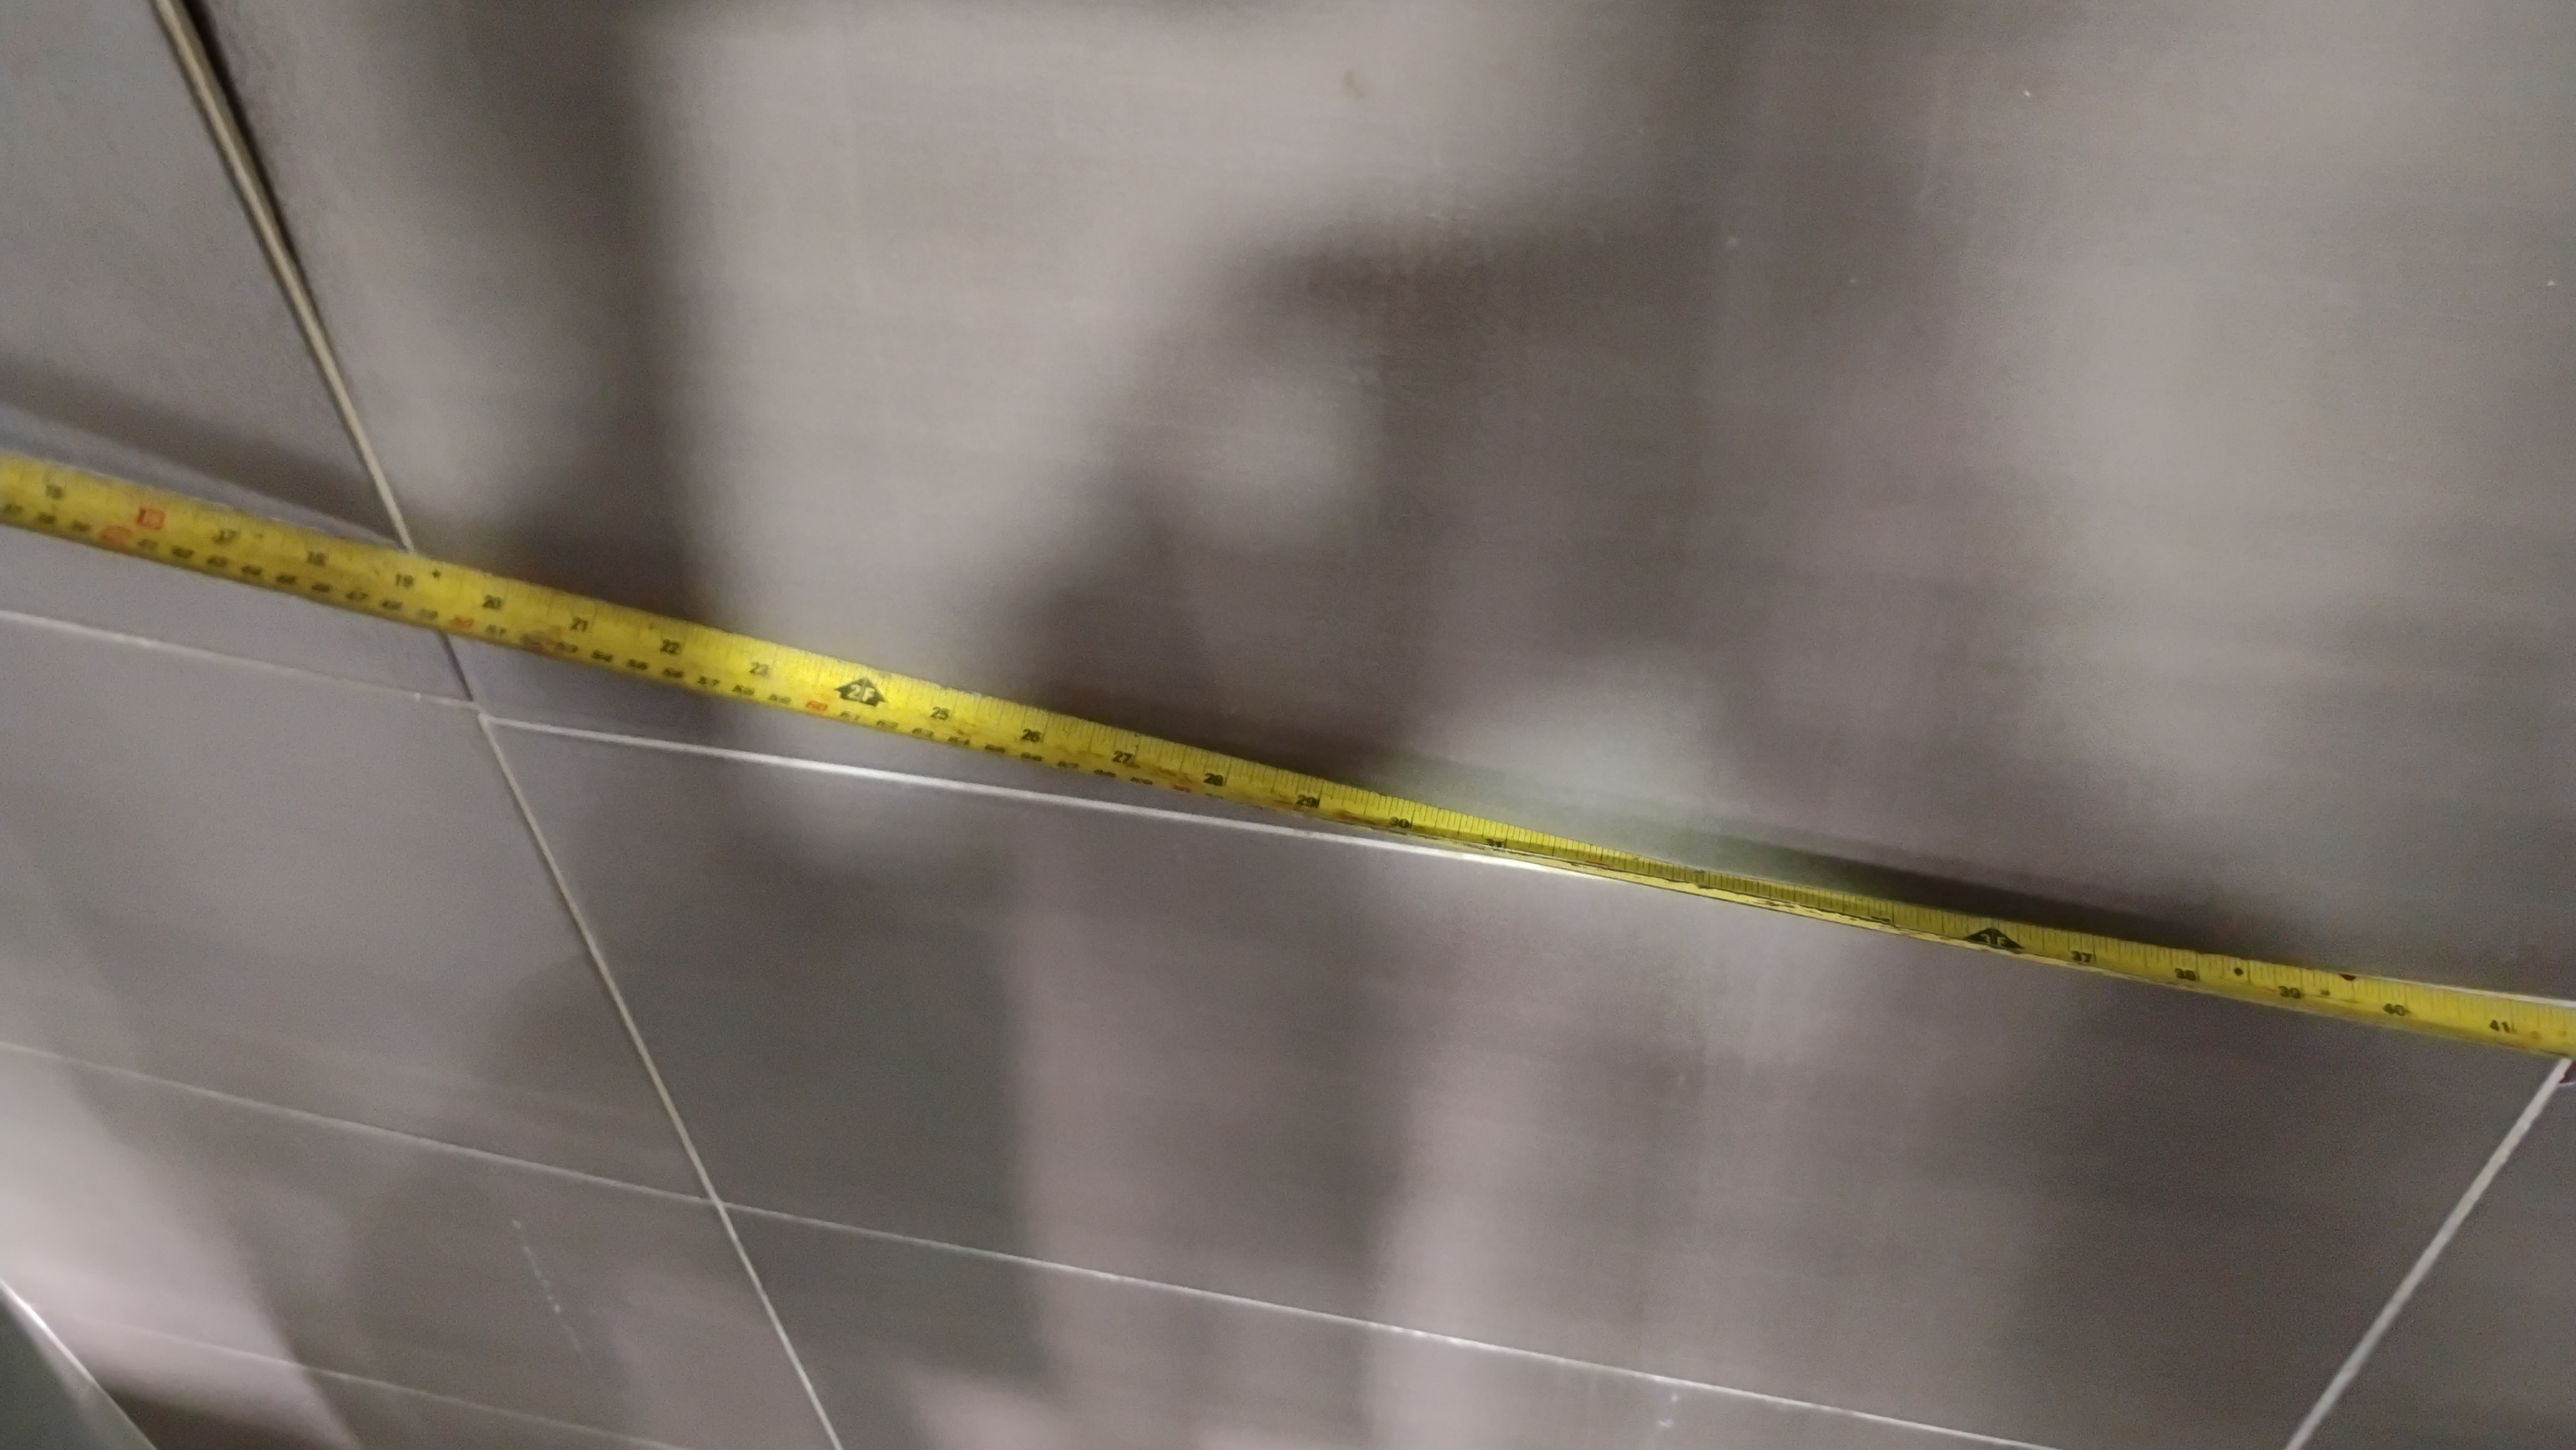
\includegraphics[width=\linewidth]{../img/IMG_20251109_150934171.jpg}\\[2pt]{\footnotesize\color{primary!60!black}Foto~8 -- 15:09:34}} \\[4pt]
\parbox{0.45\textwidth}{\centering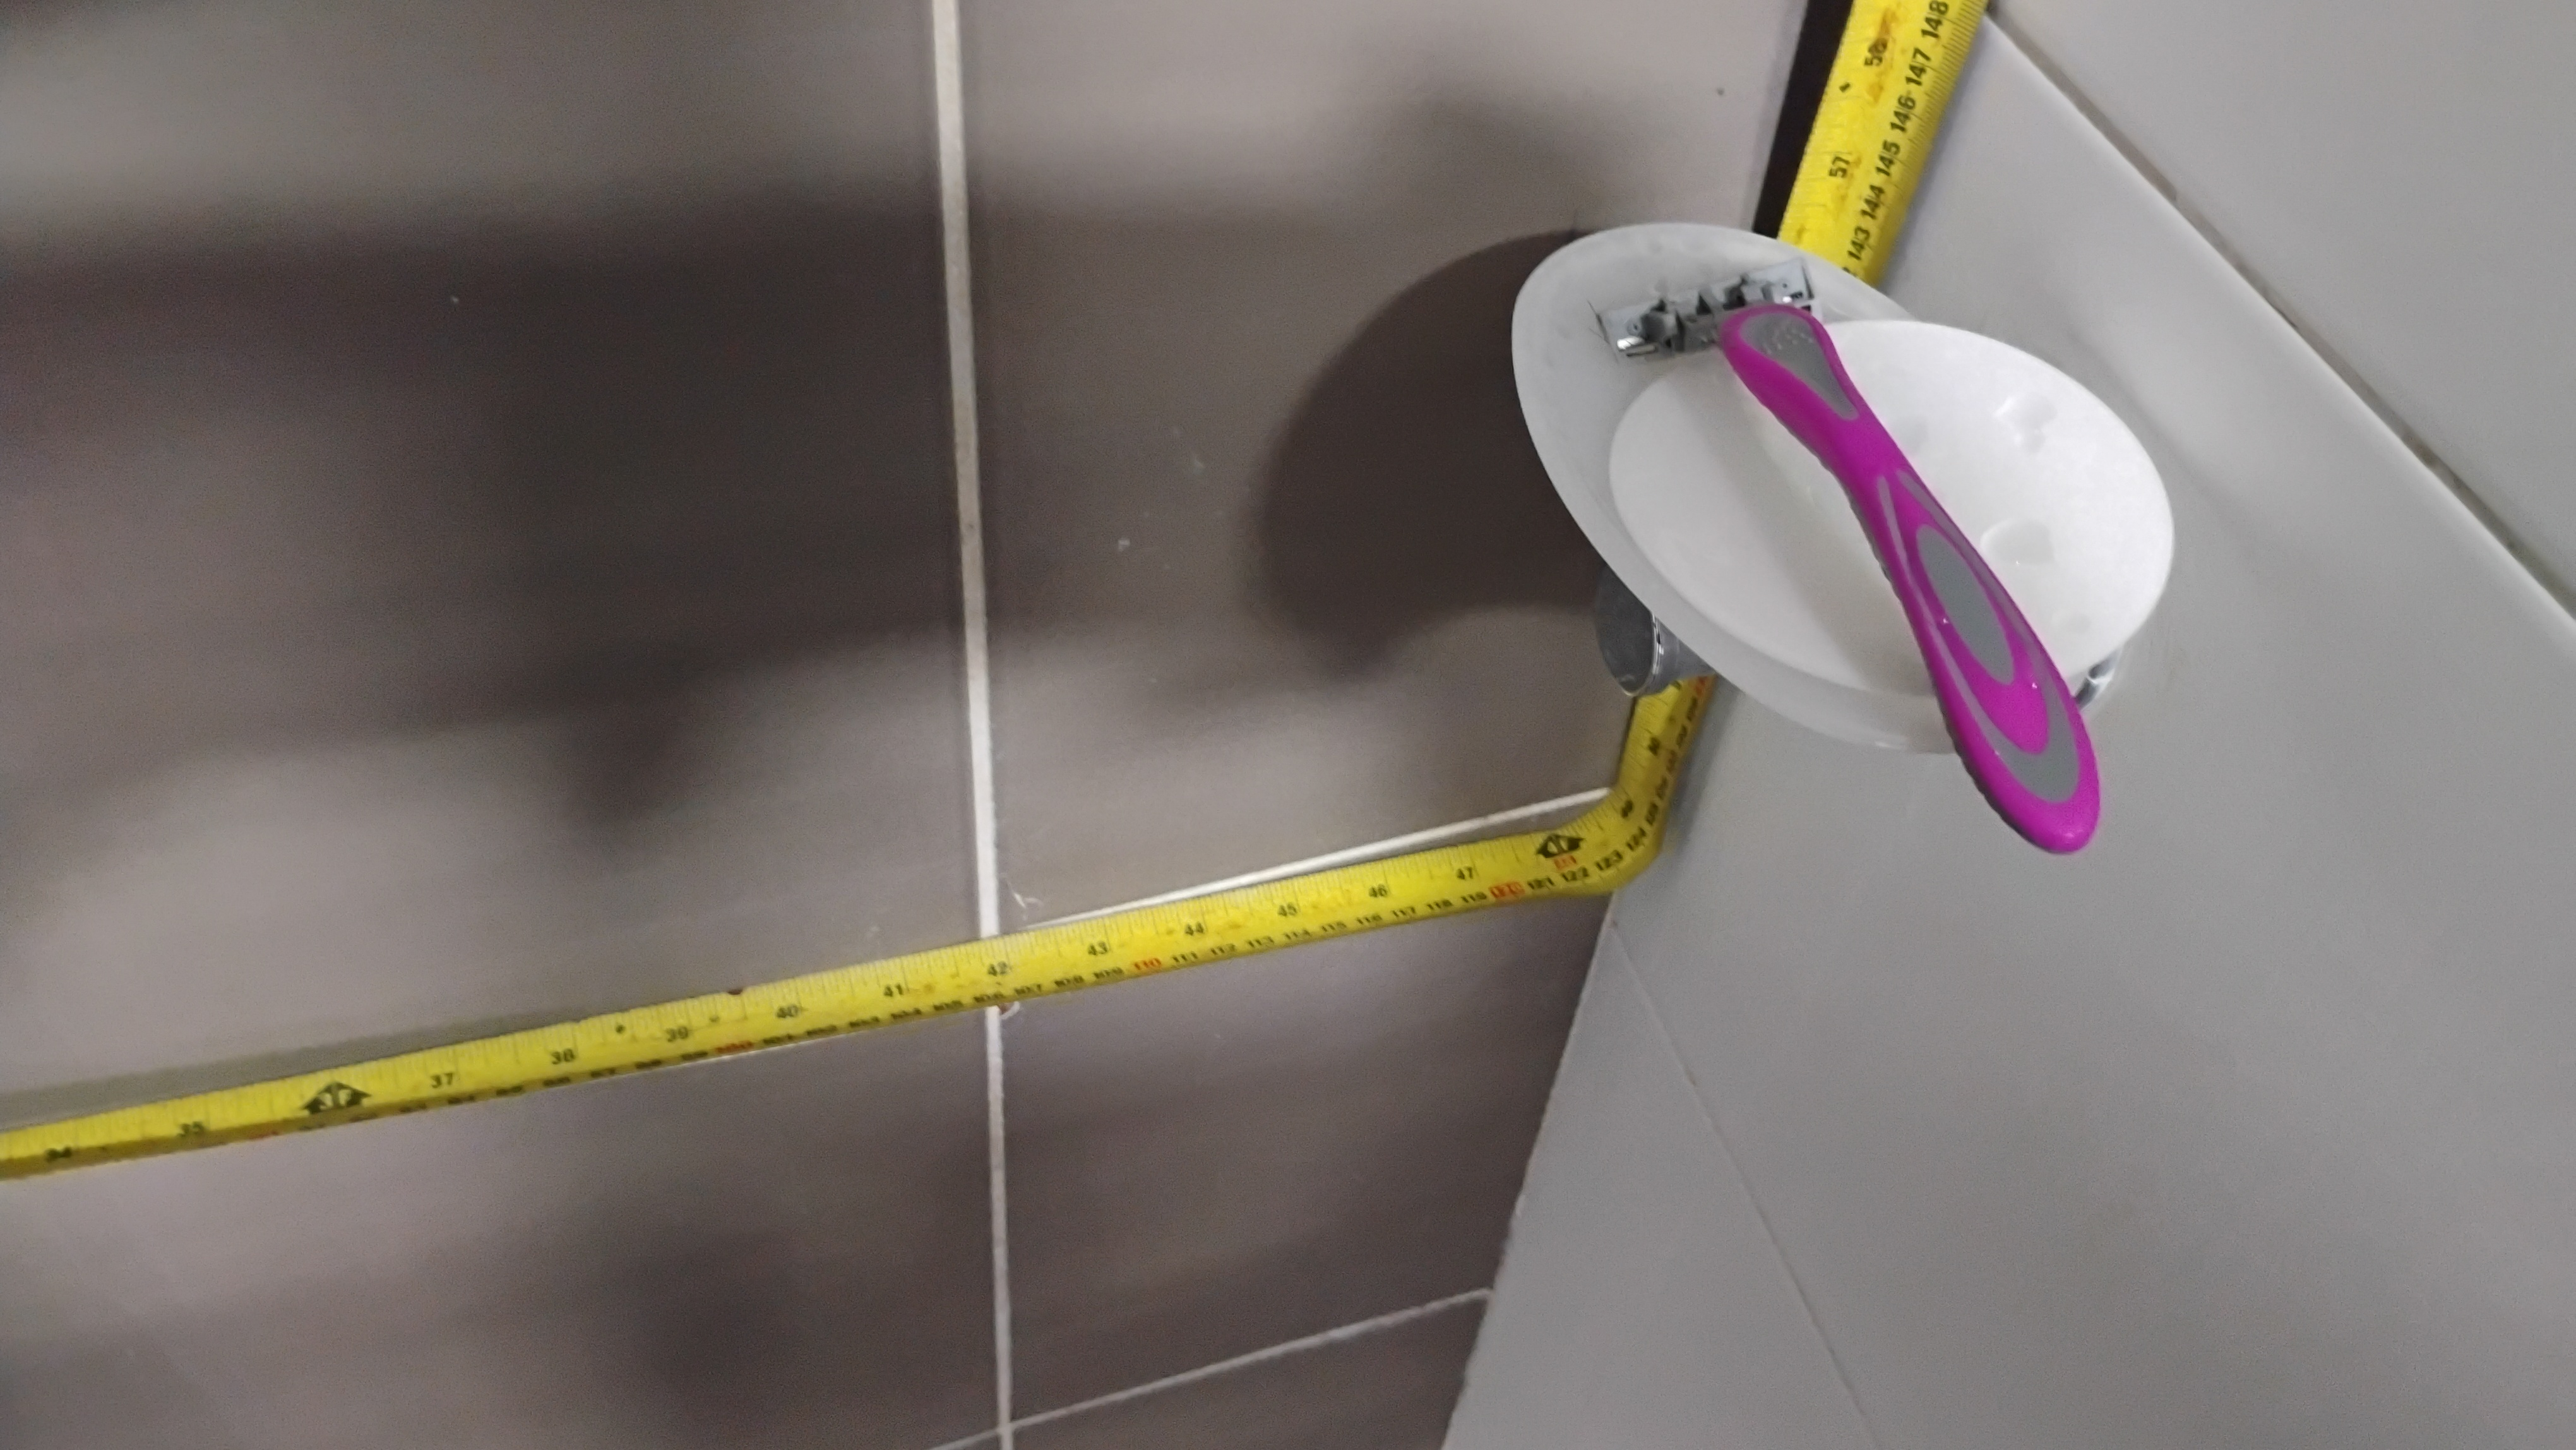
\includegraphics[width=\linewidth]{../img/IMG_20251109_150936200.jpg}\\[2pt]{\footnotesize\color{primary!60!black}Foto~9 -- 15:09:36}} & \parbox{0.45\textwidth}{\centering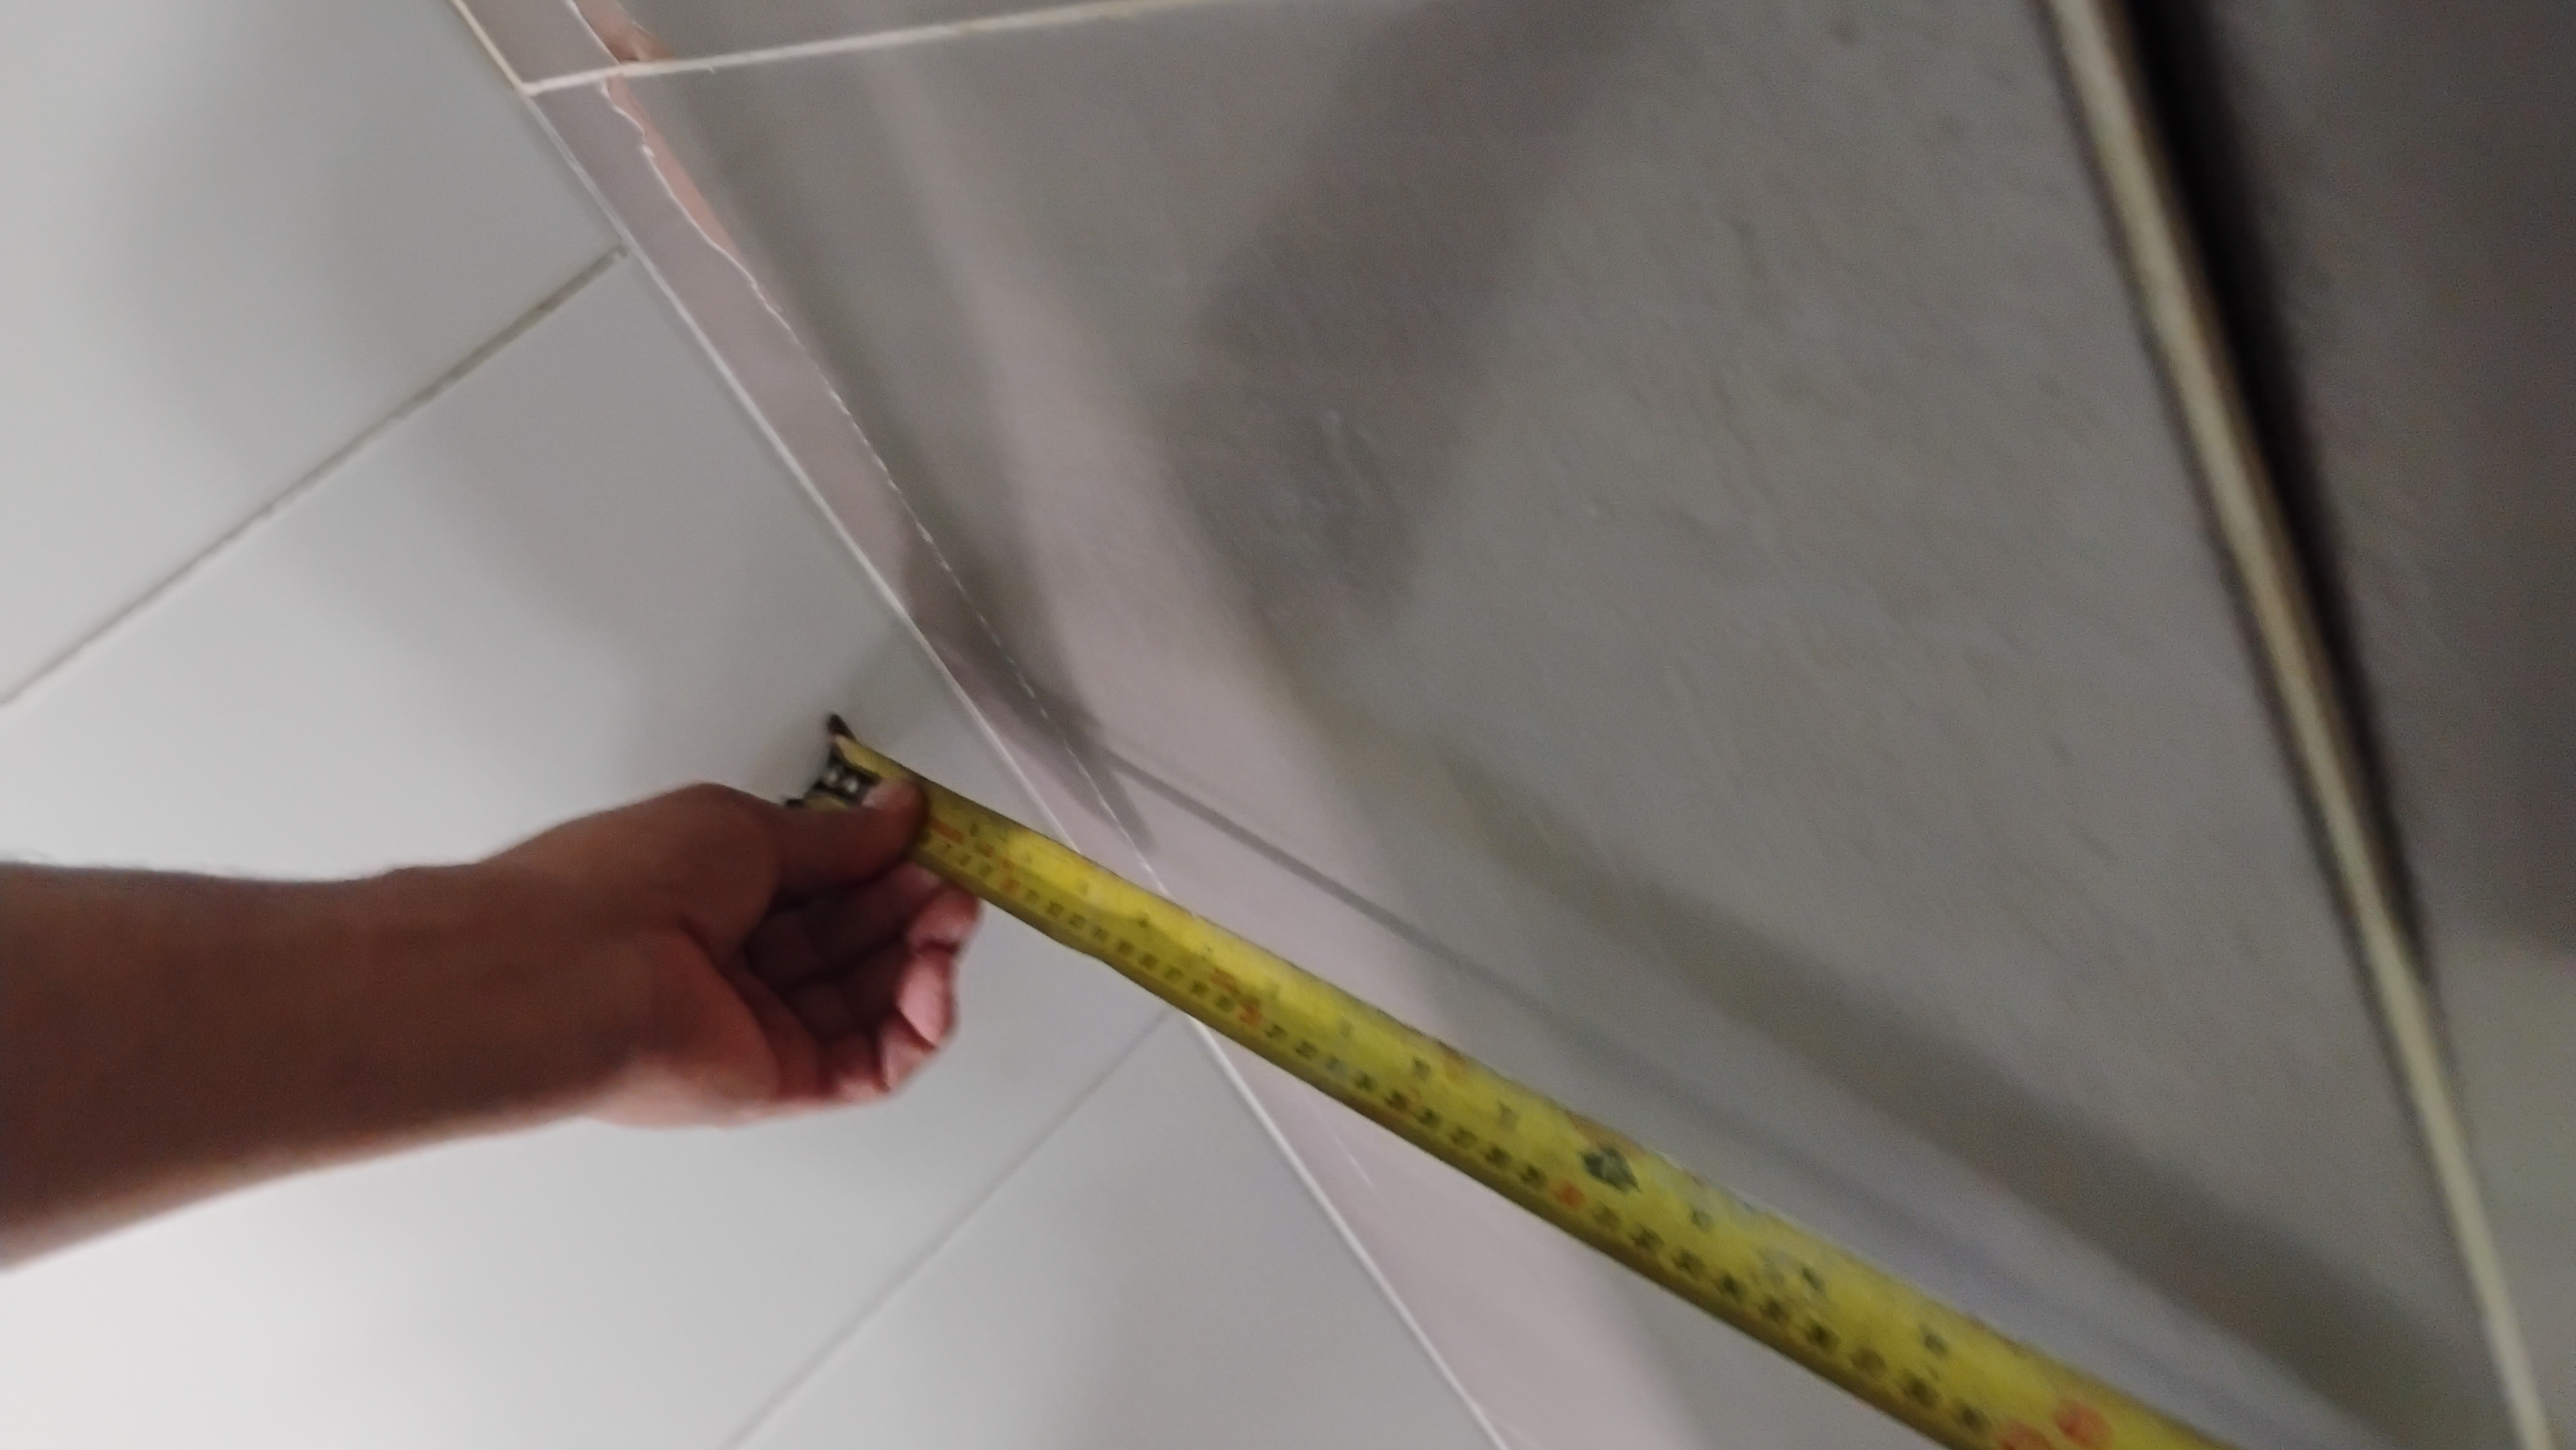
\includegraphics[width=\linewidth]{../img/IMG_20251109_150948191.jpg}\\[2pt]{\footnotesize\color{primary!60!black}Foto~10 -- 15:09:48}} \\[4pt]
\parbox{0.45\textwidth}{\centering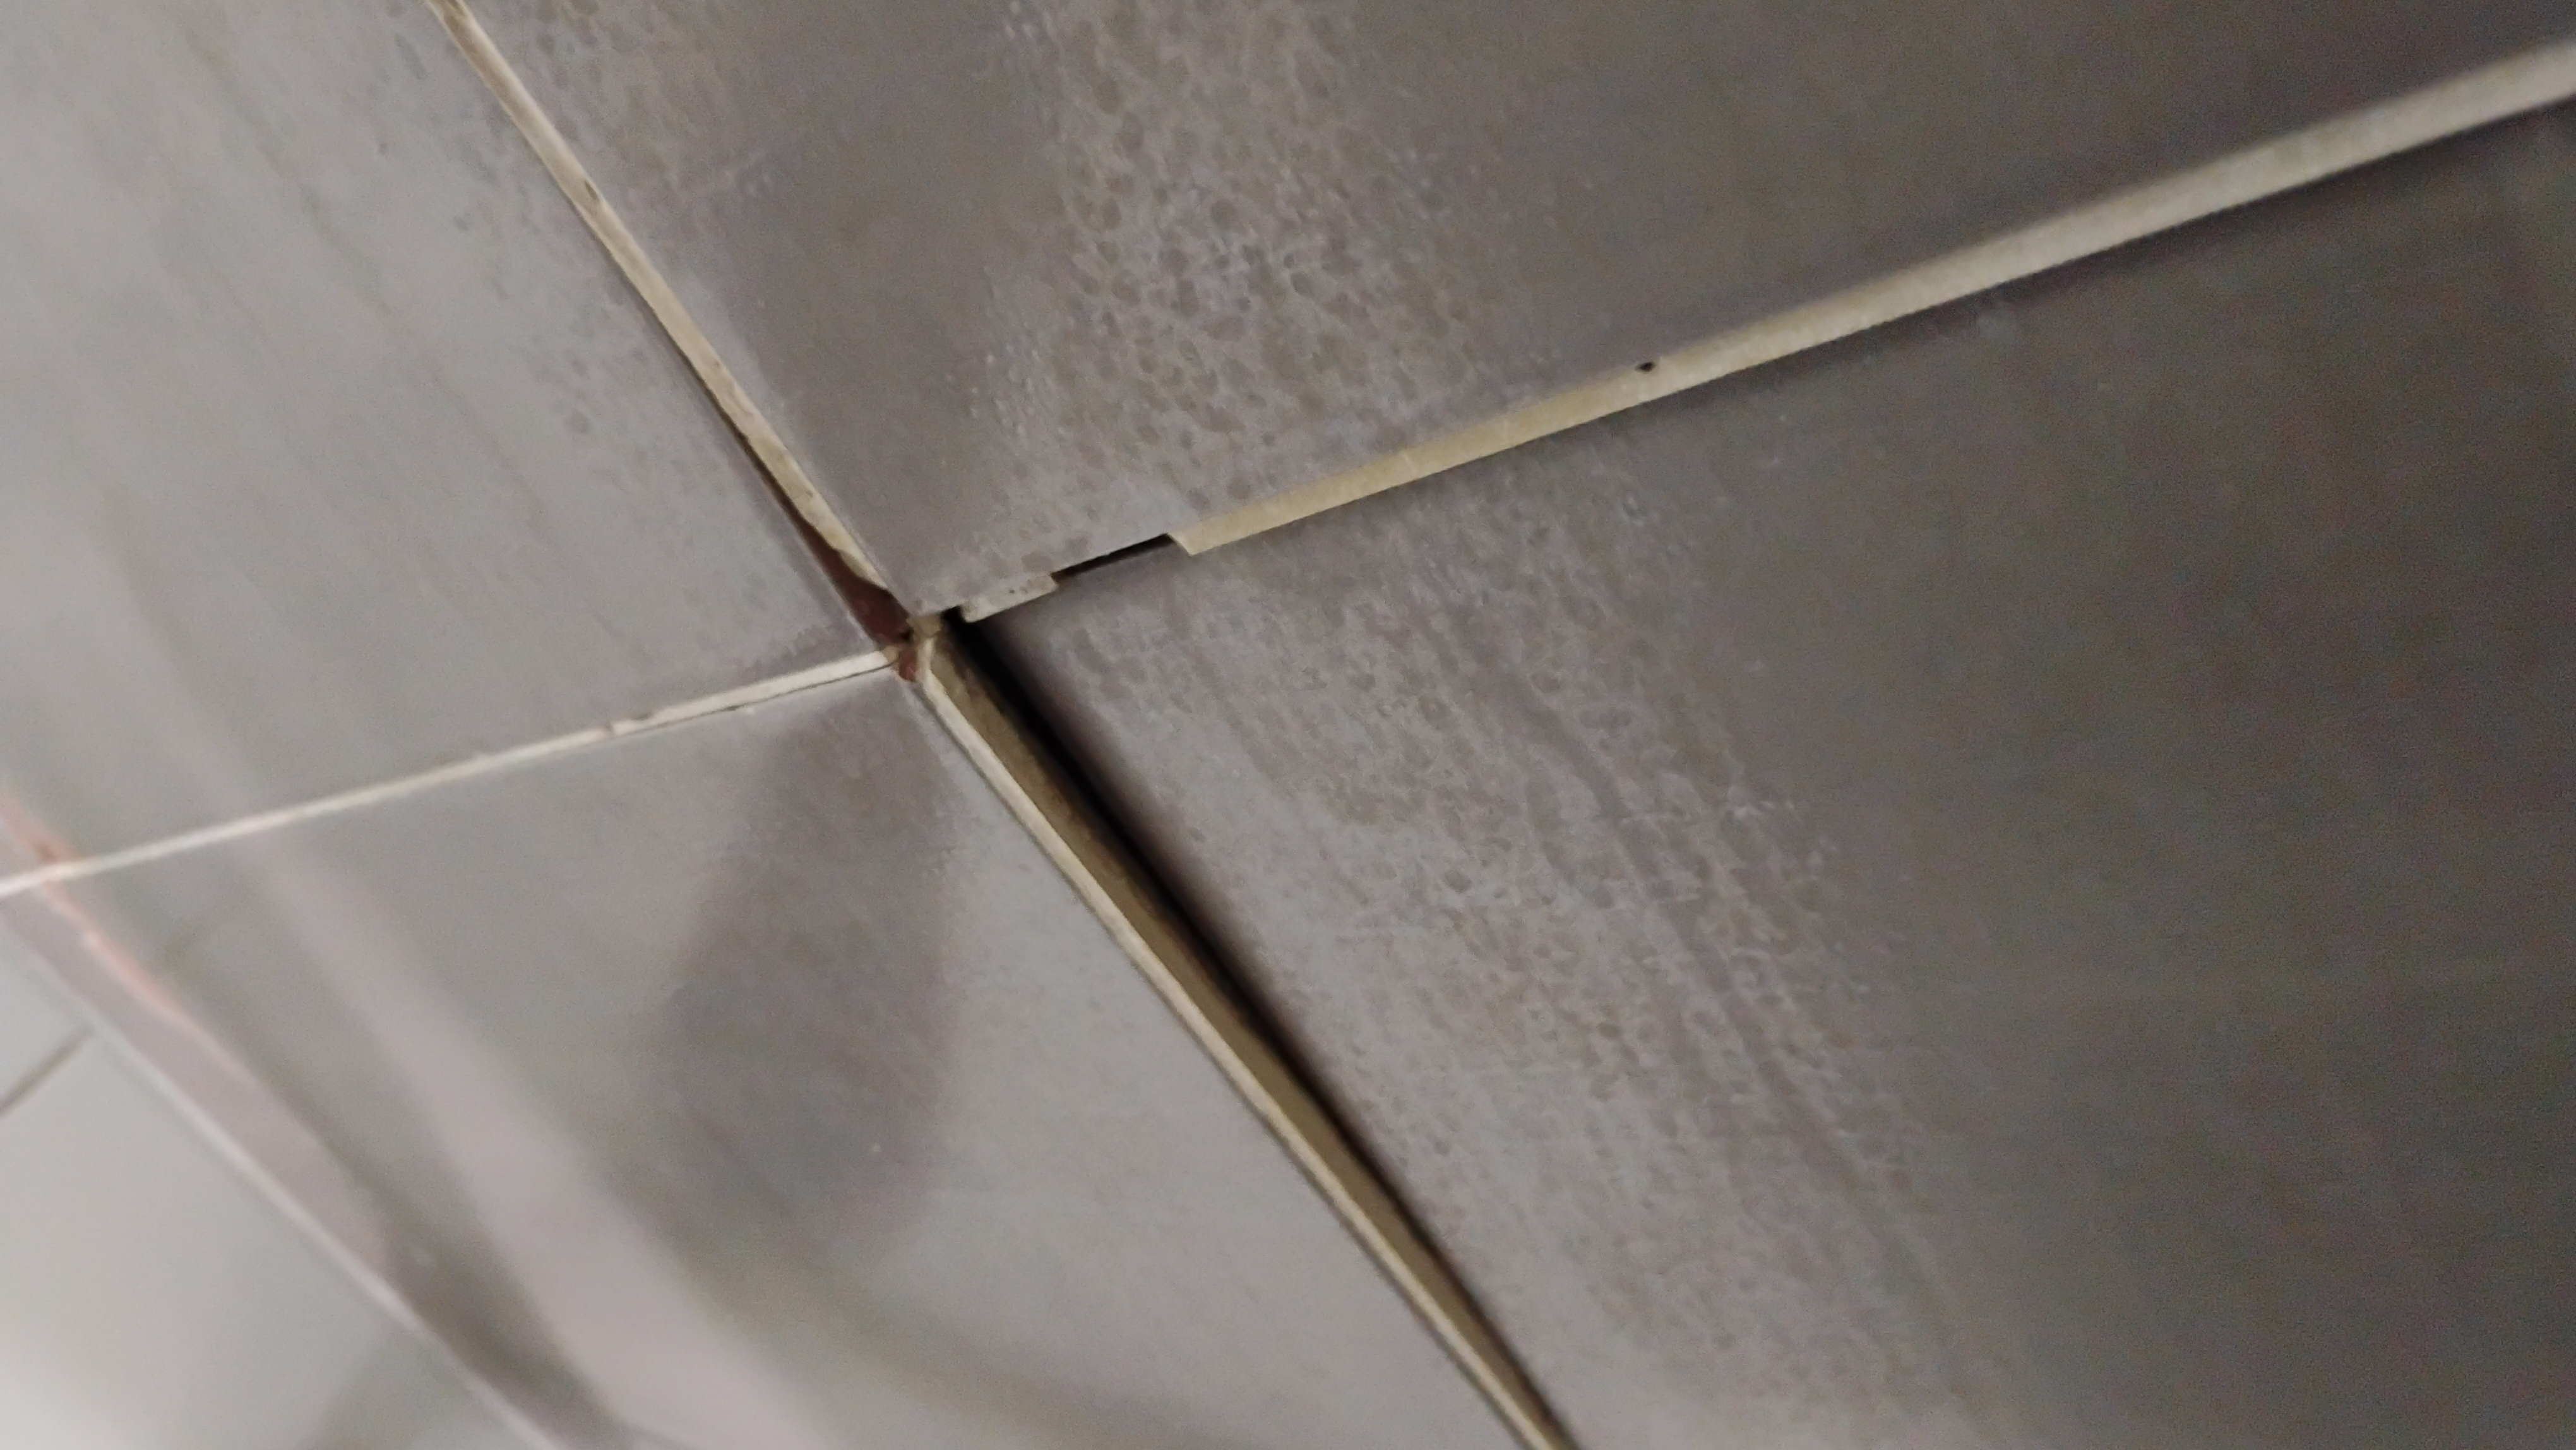
\includegraphics[width=\linewidth]{../img/IMG_20251109_150951284.jpg}\\[2pt]{\footnotesize\color{primary!60!black}Foto~11 -- 15:09:51}} & \parbox{0.45\textwidth}{\centering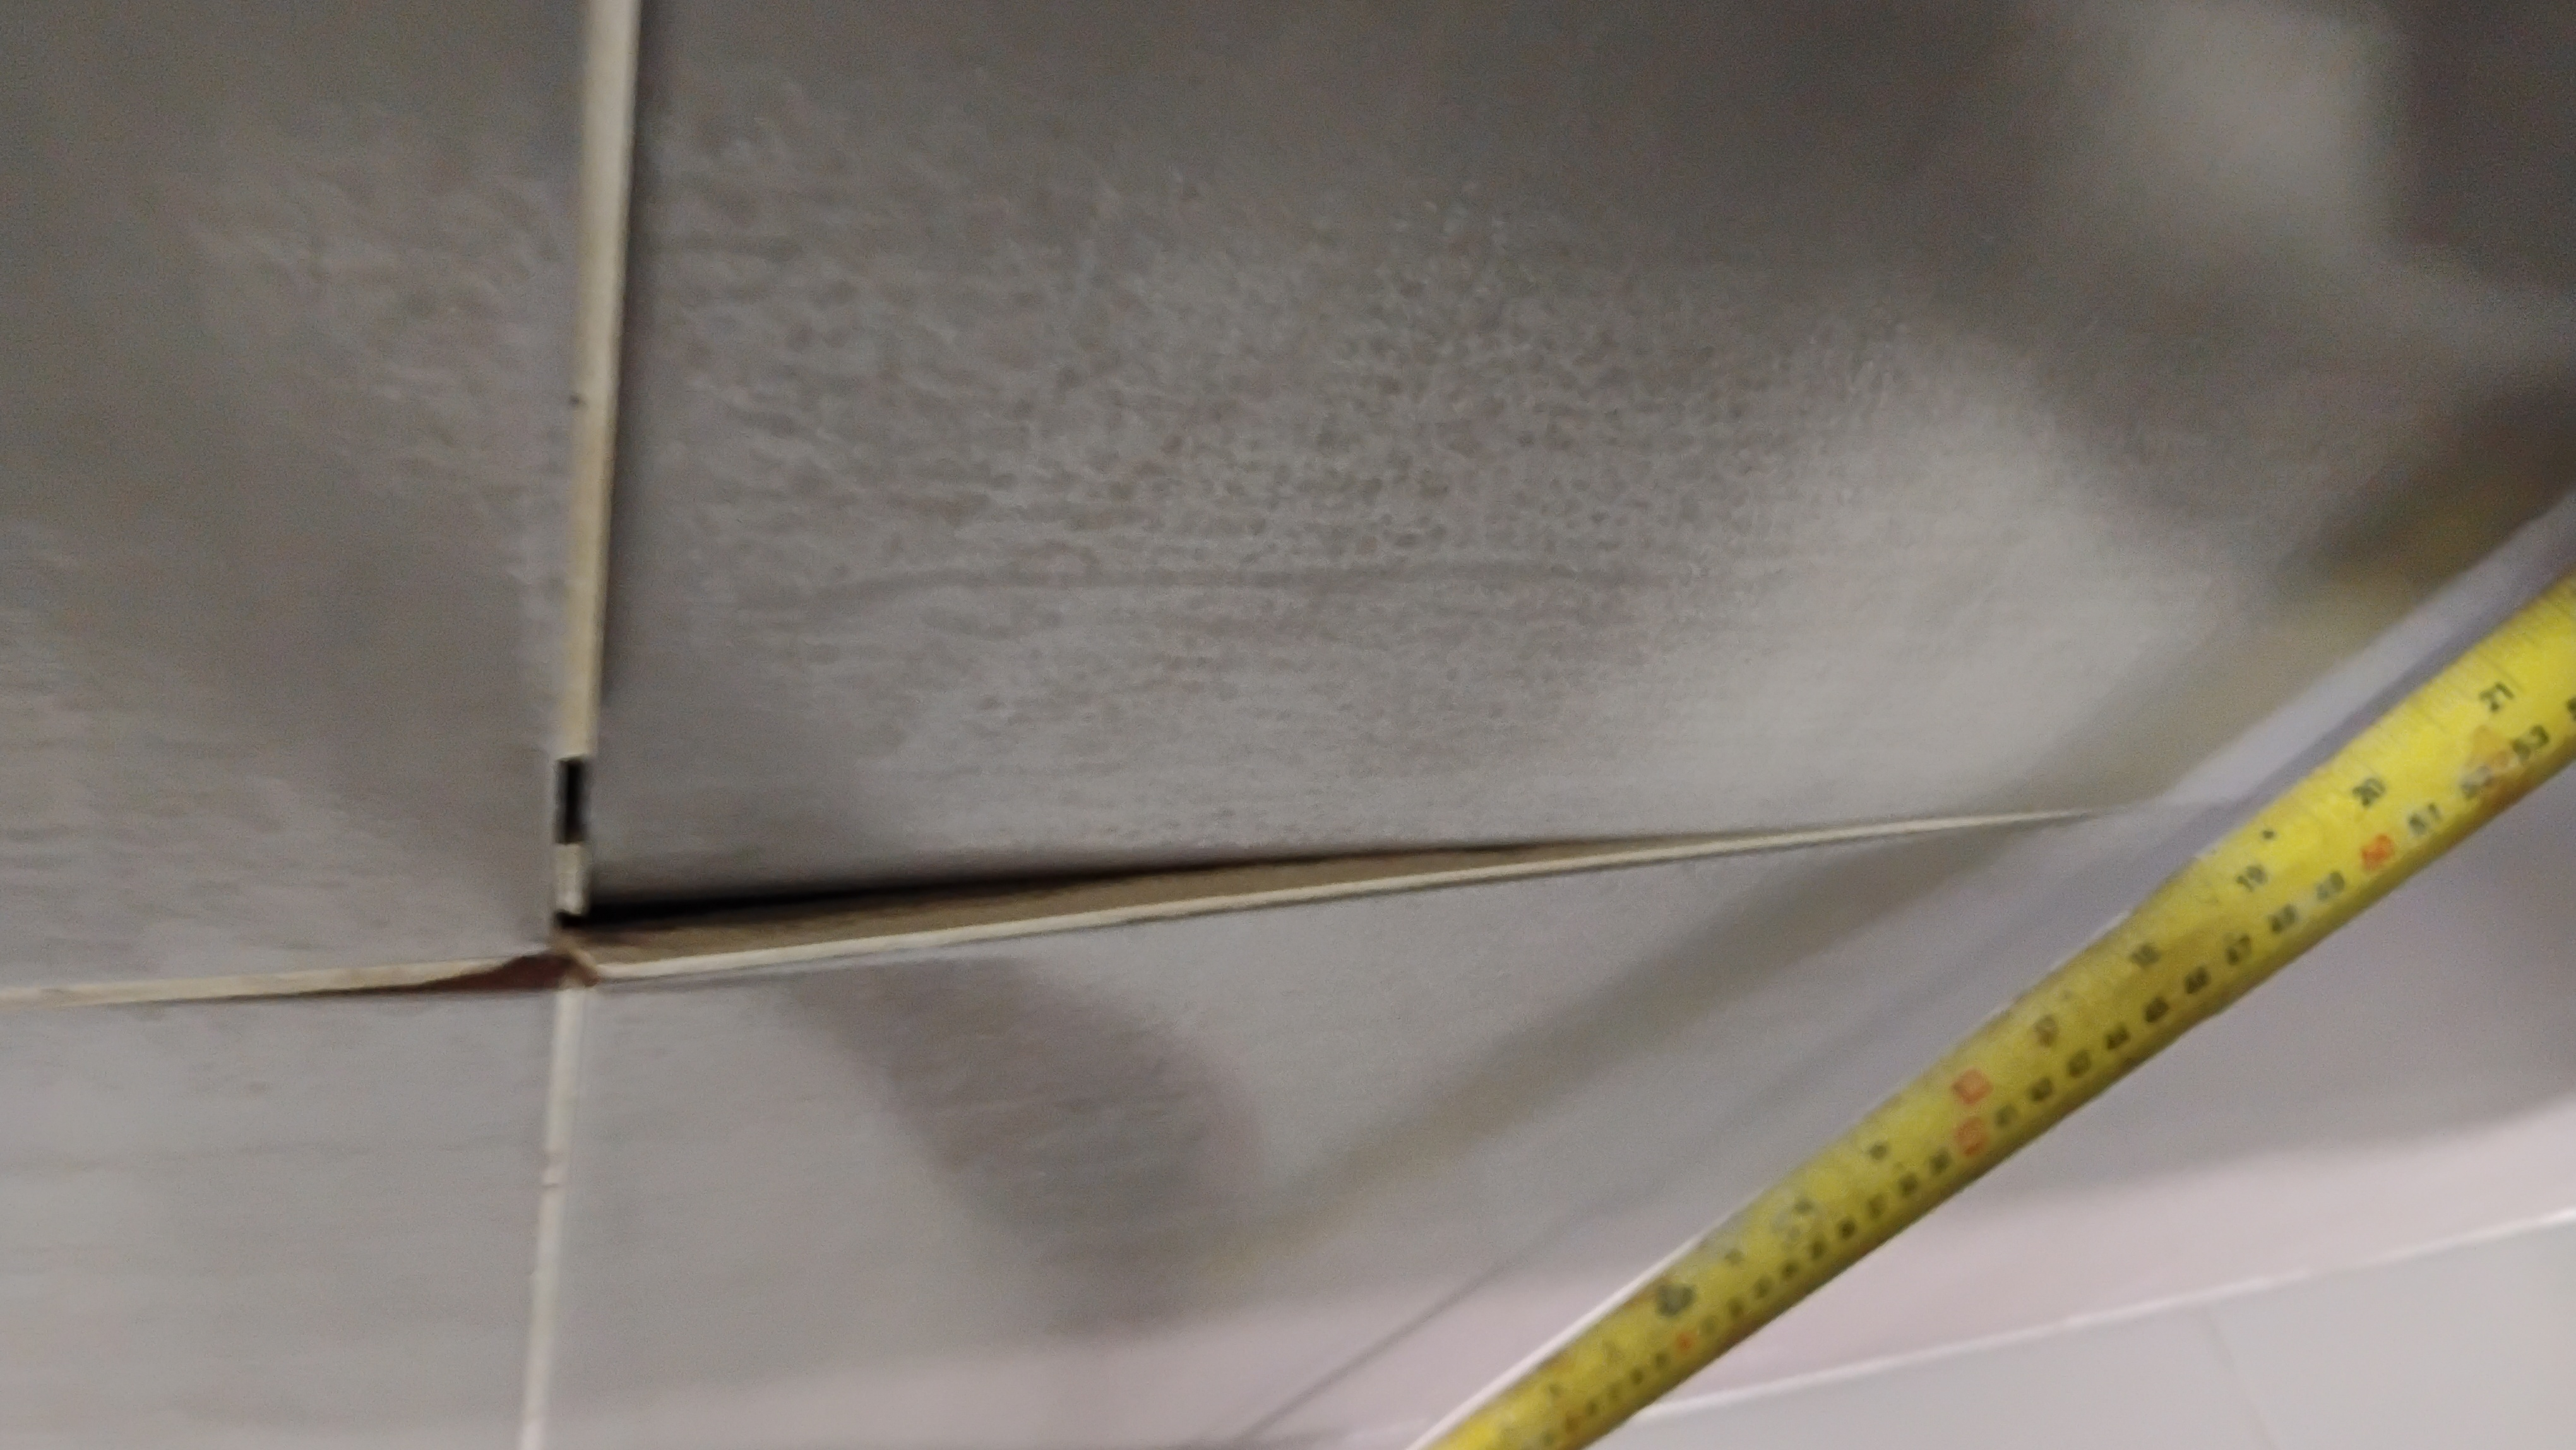
\includegraphics[width=\linewidth]{../img/IMG_20251109_150953979.jpg}\\[2pt]{\footnotesize\color{primary!60!black}Foto~12 -- 15:09:53}} \\[4pt]
\end{tabular}
\caption{Paramento Norte — Desprendimiento de Enchape Cerámico: Fotos 7 al 12.}\end{figure}
\newpage
\begin{figure}[H]
\centering
\begin{tabular}{cc}
\parbox{0.45\textwidth}{\centering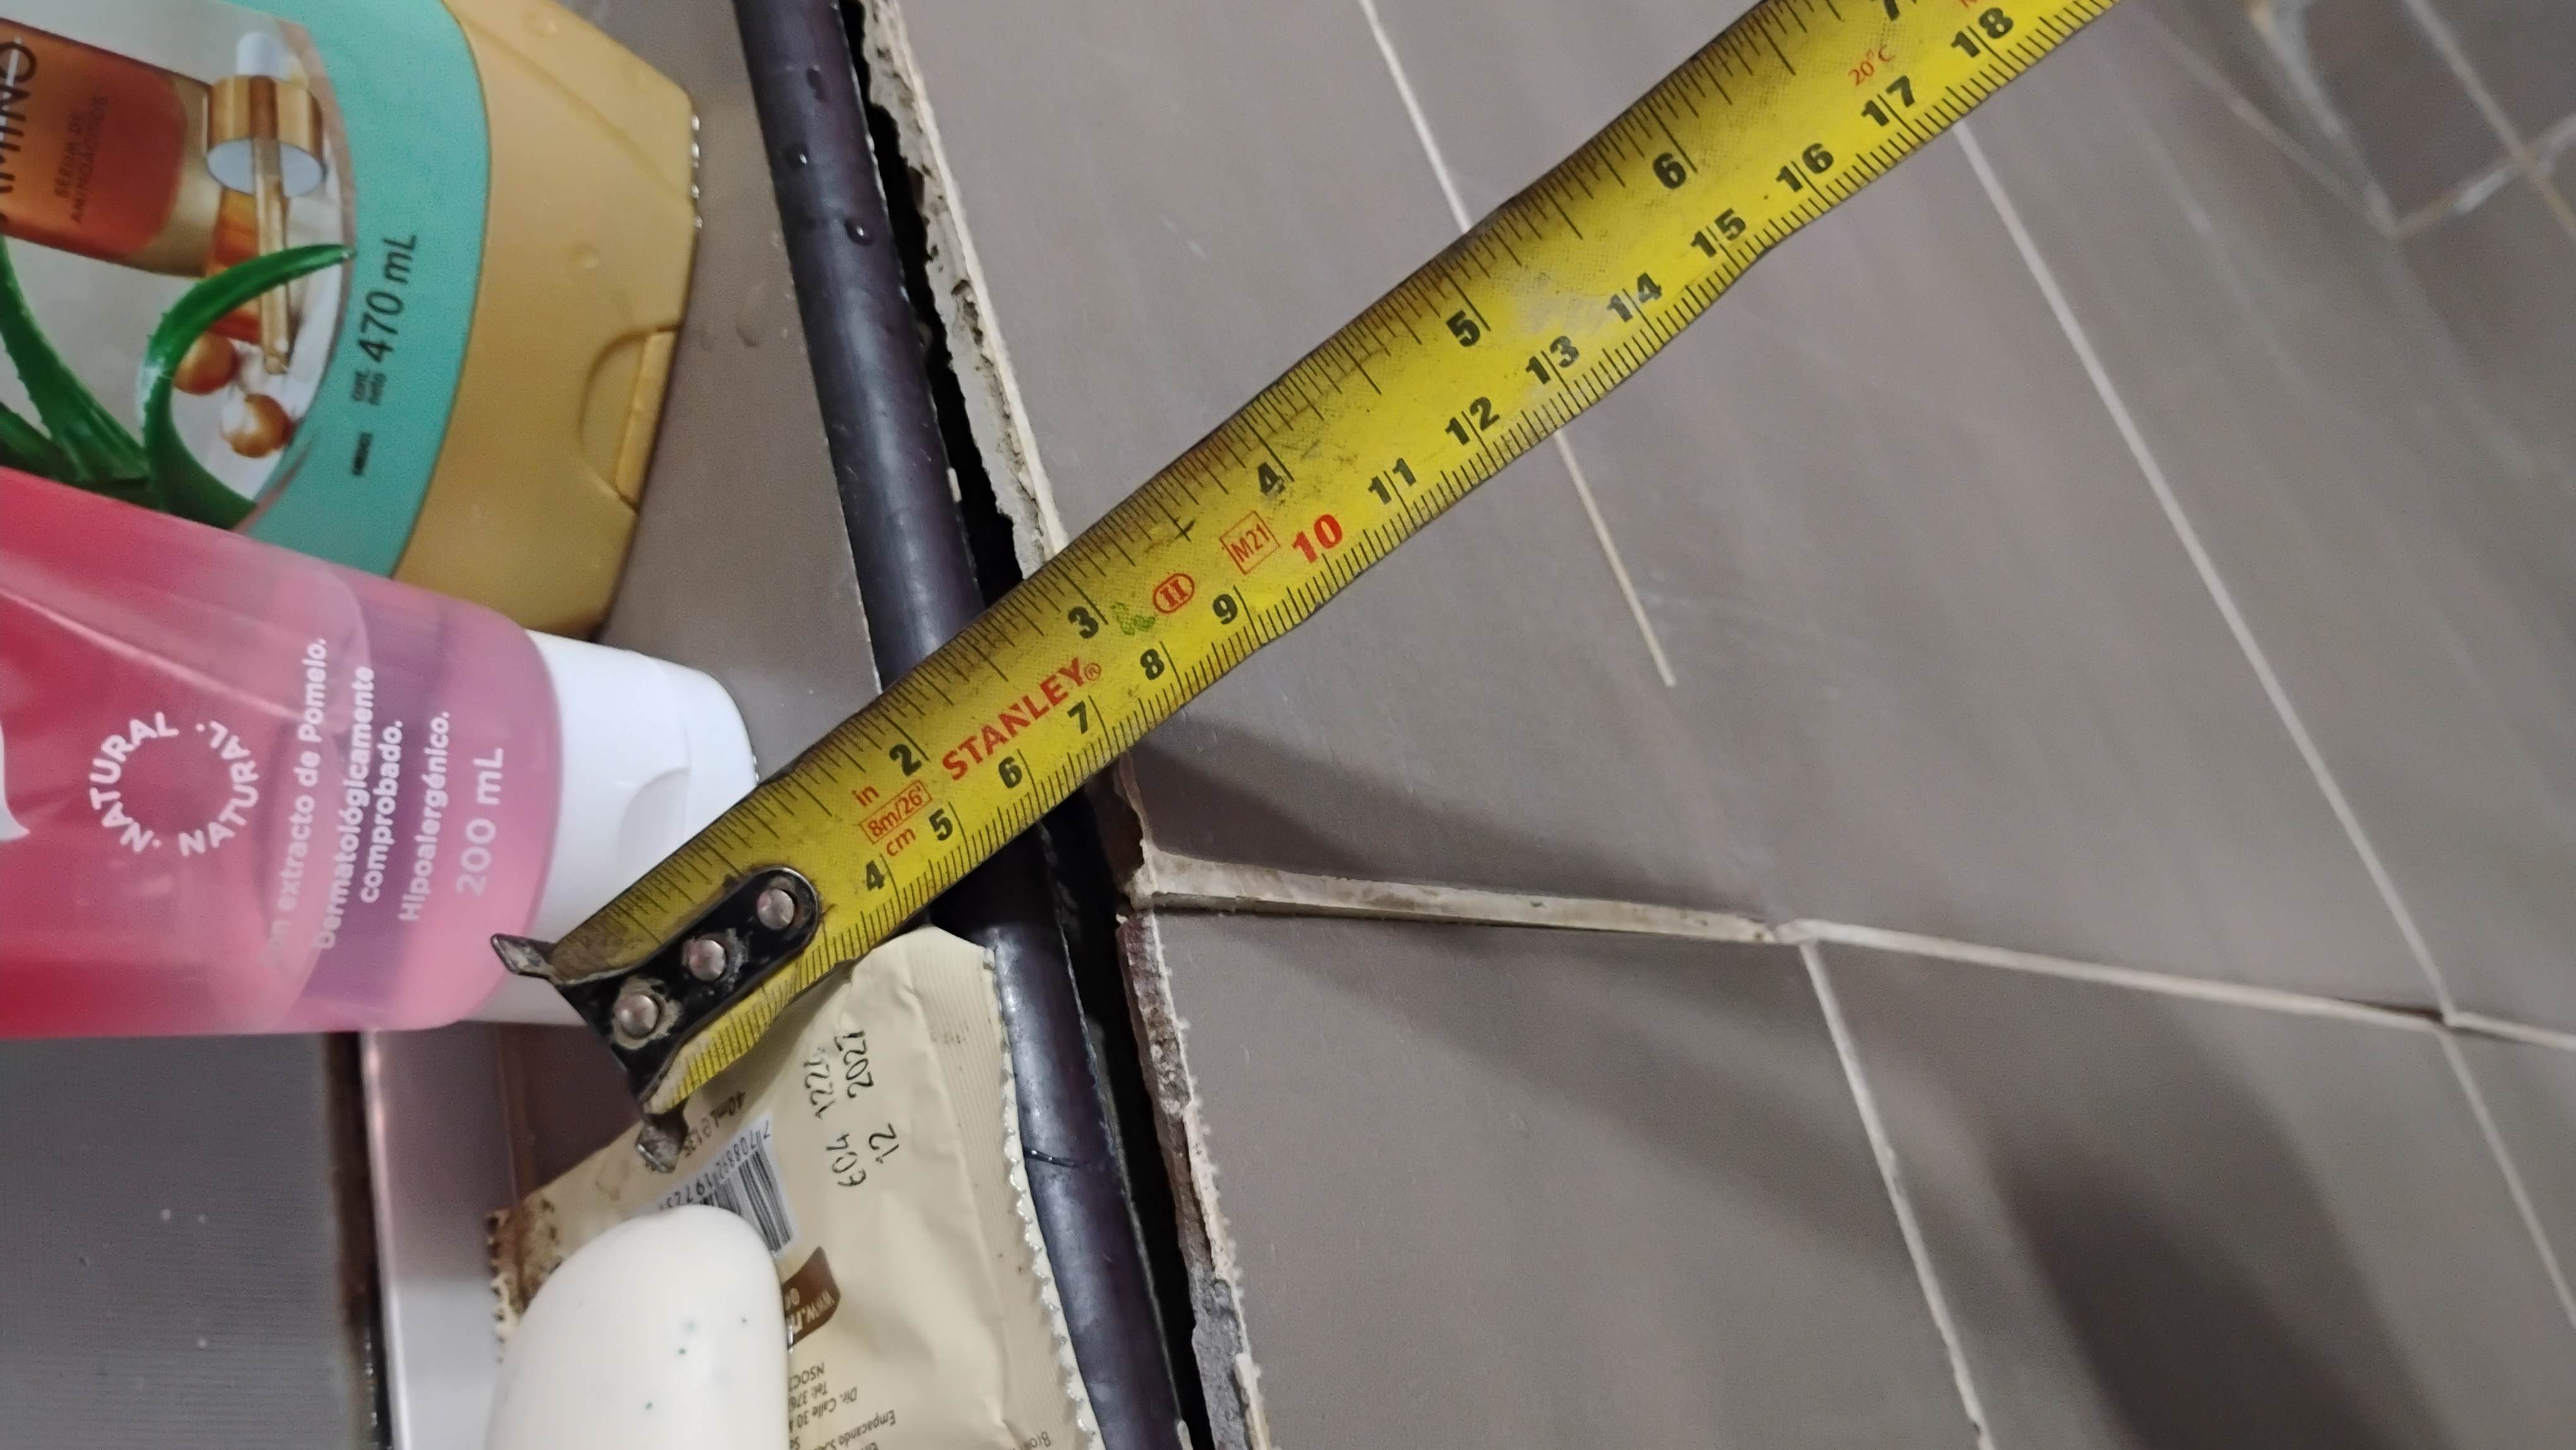
\includegraphics[width=\linewidth]{../img/IMG_20251109_151024233.jpg}\\[2pt]{\footnotesize\color{primary!60!black}Foto~13 -- 15:10:24}} & \parbox{0.45\textwidth}{\centering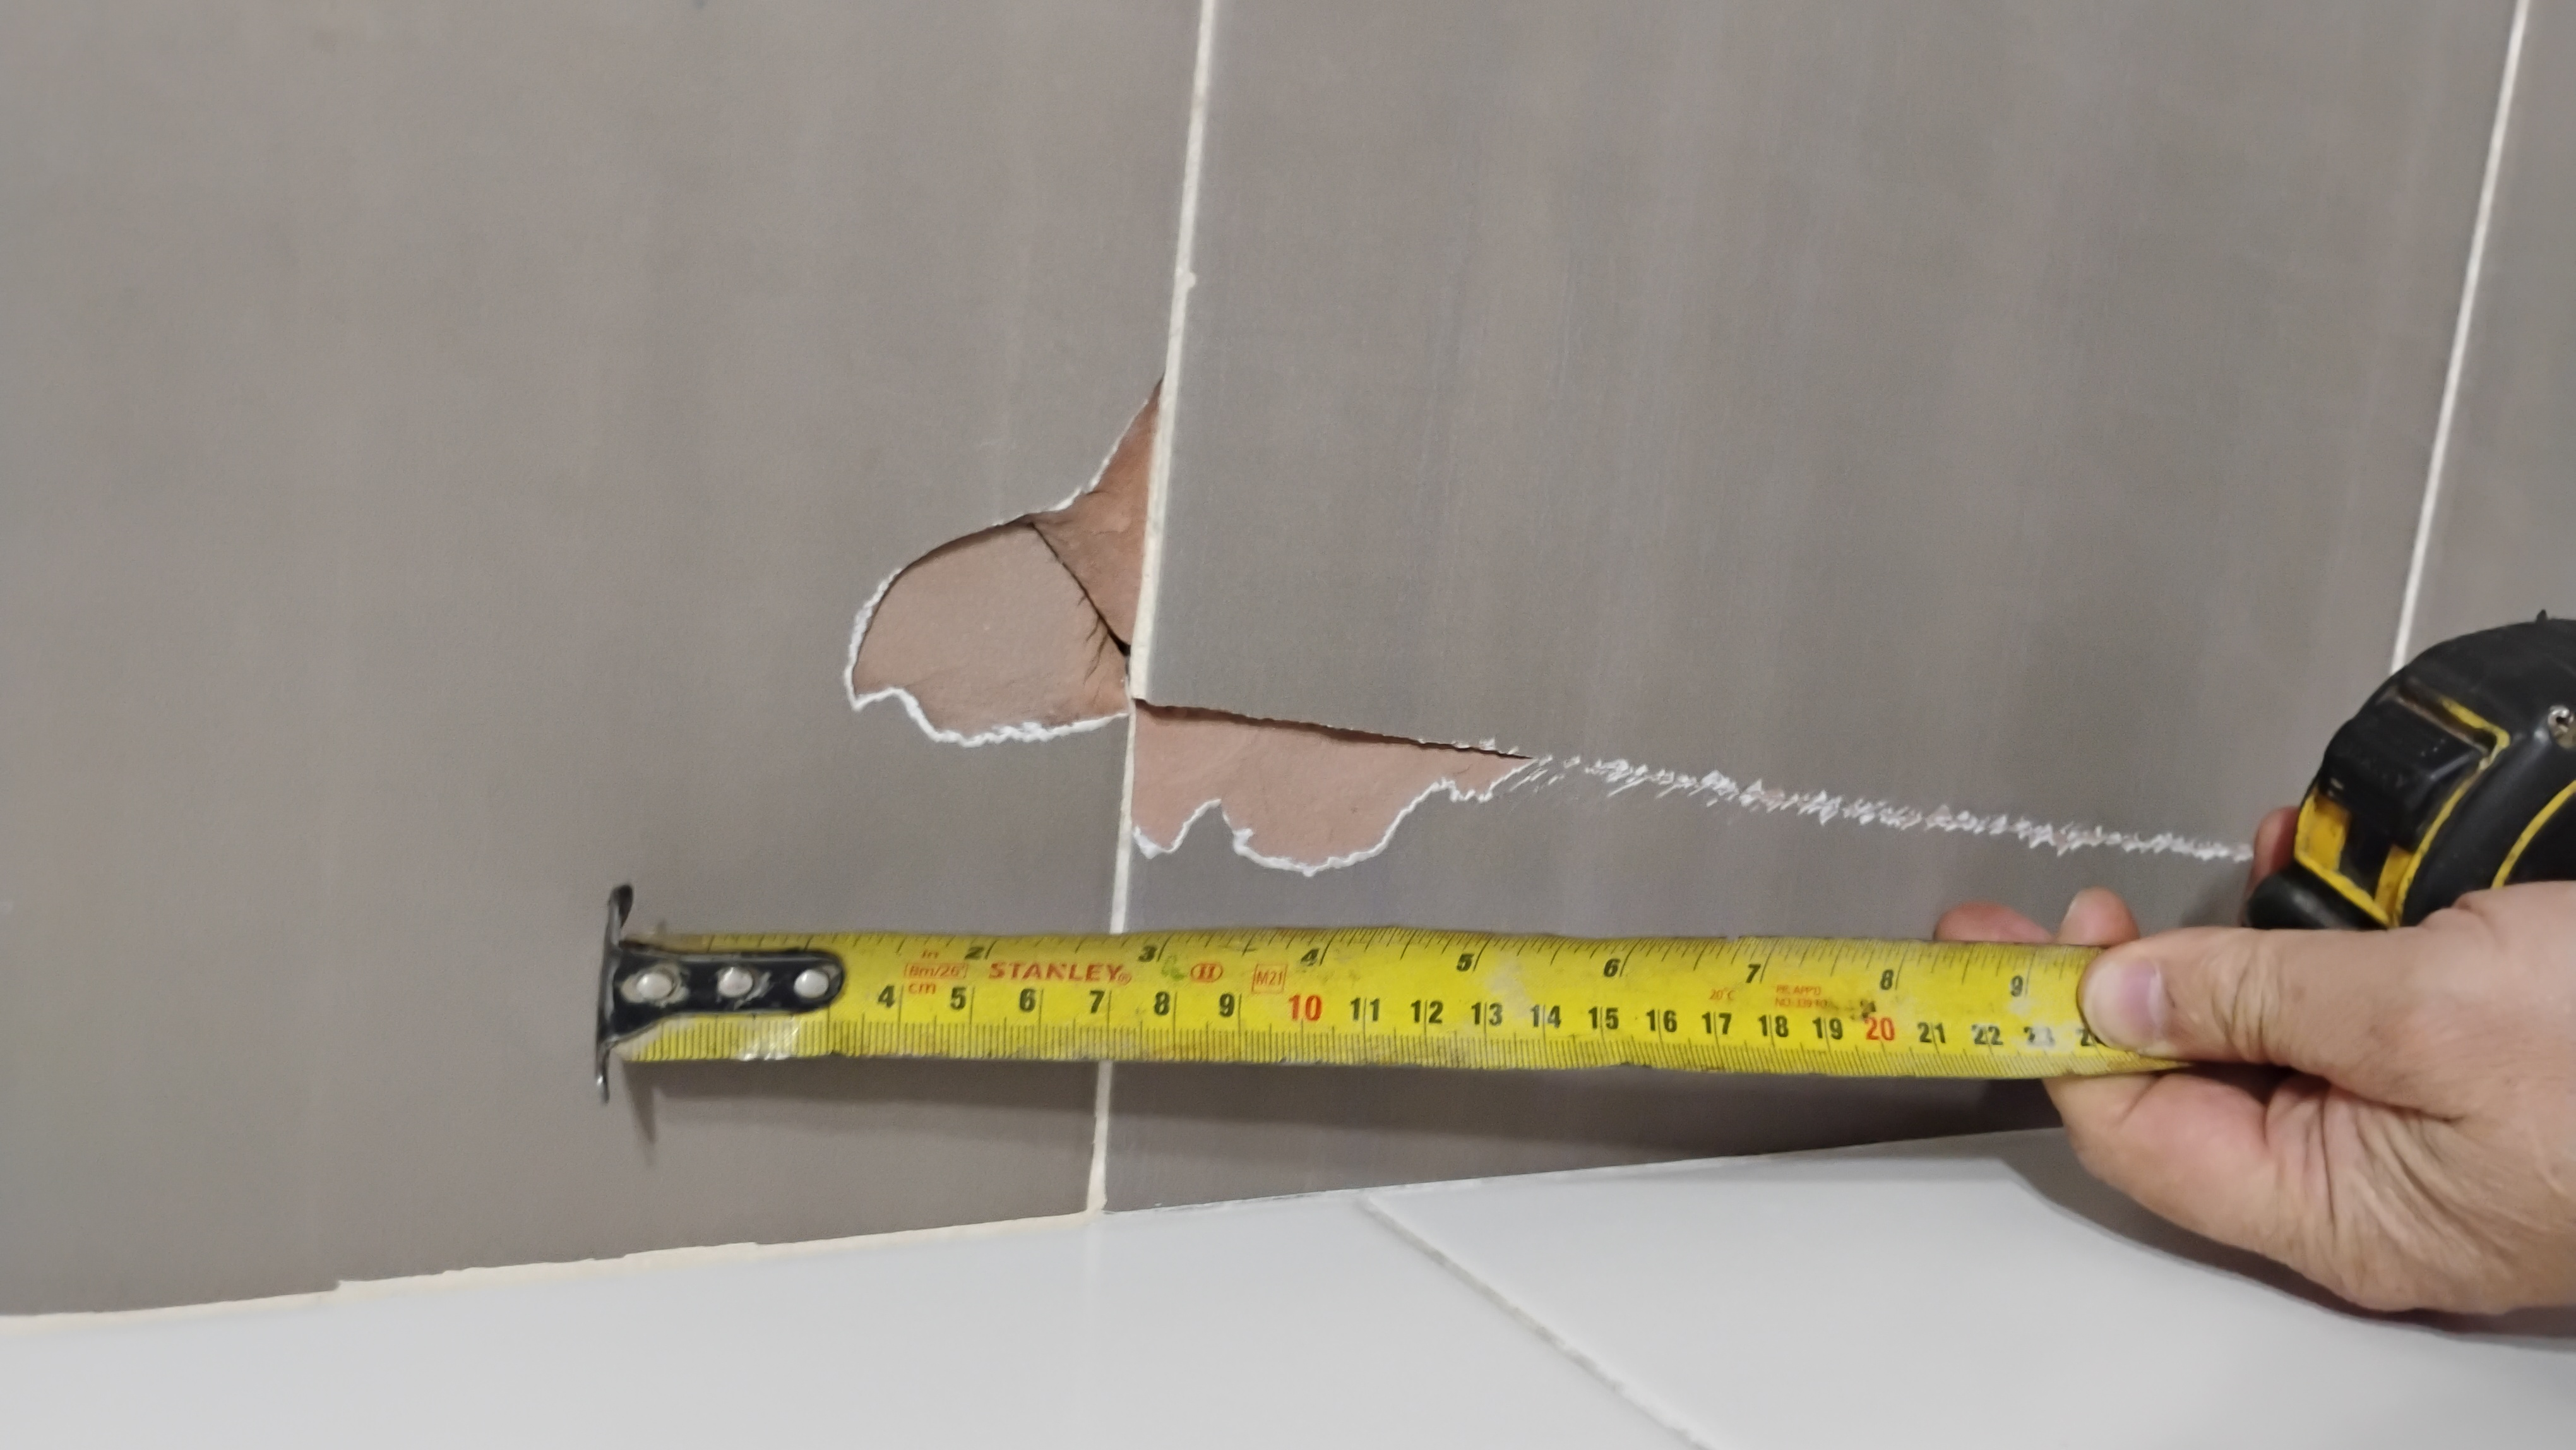
\includegraphics[width=\linewidth]{../img/IMG_20251109_151036830.jpg}\\[2pt]{\footnotesize\color{primary!60!black}Foto~14 -- 15:10:36}} \\[4pt]
\parbox{0.45\textwidth}{\centering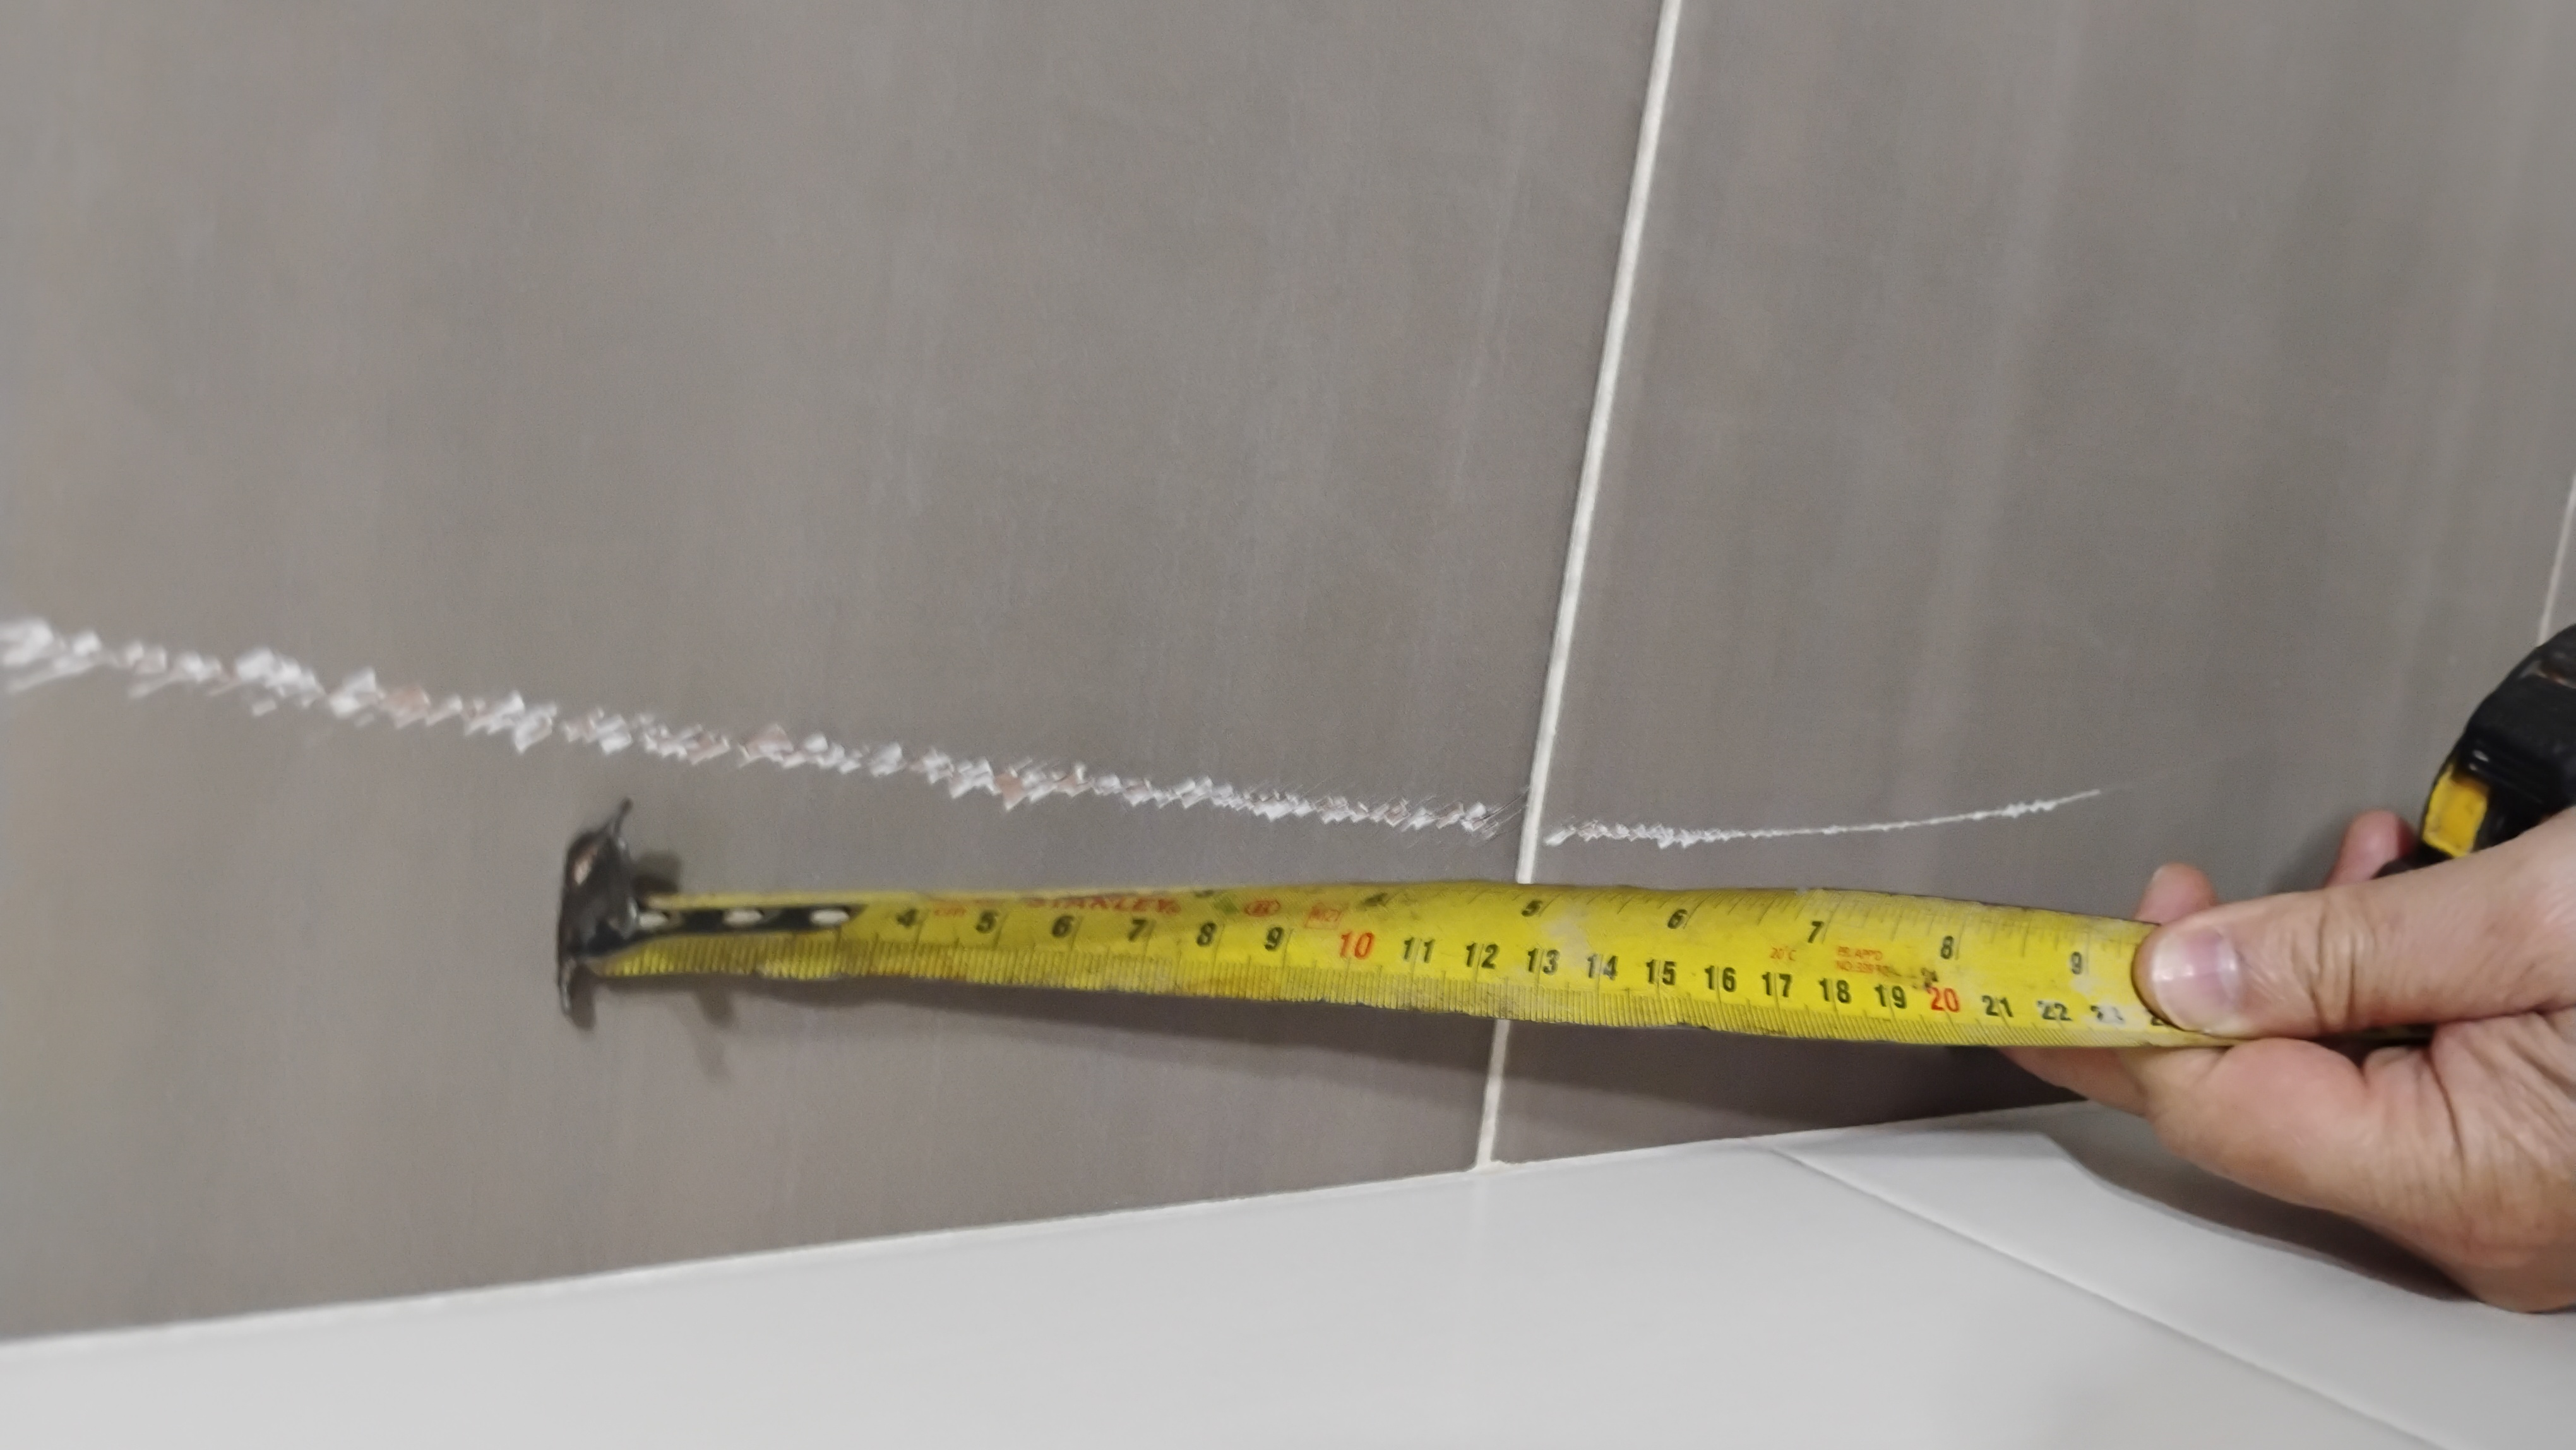
\includegraphics[width=\linewidth]{../img/IMG_20251109_151042772.jpg}\\[2pt]{\footnotesize\color{primary!60!black}Foto~15 -- 15:10:42}} & \parbox{0.45\textwidth}{\centering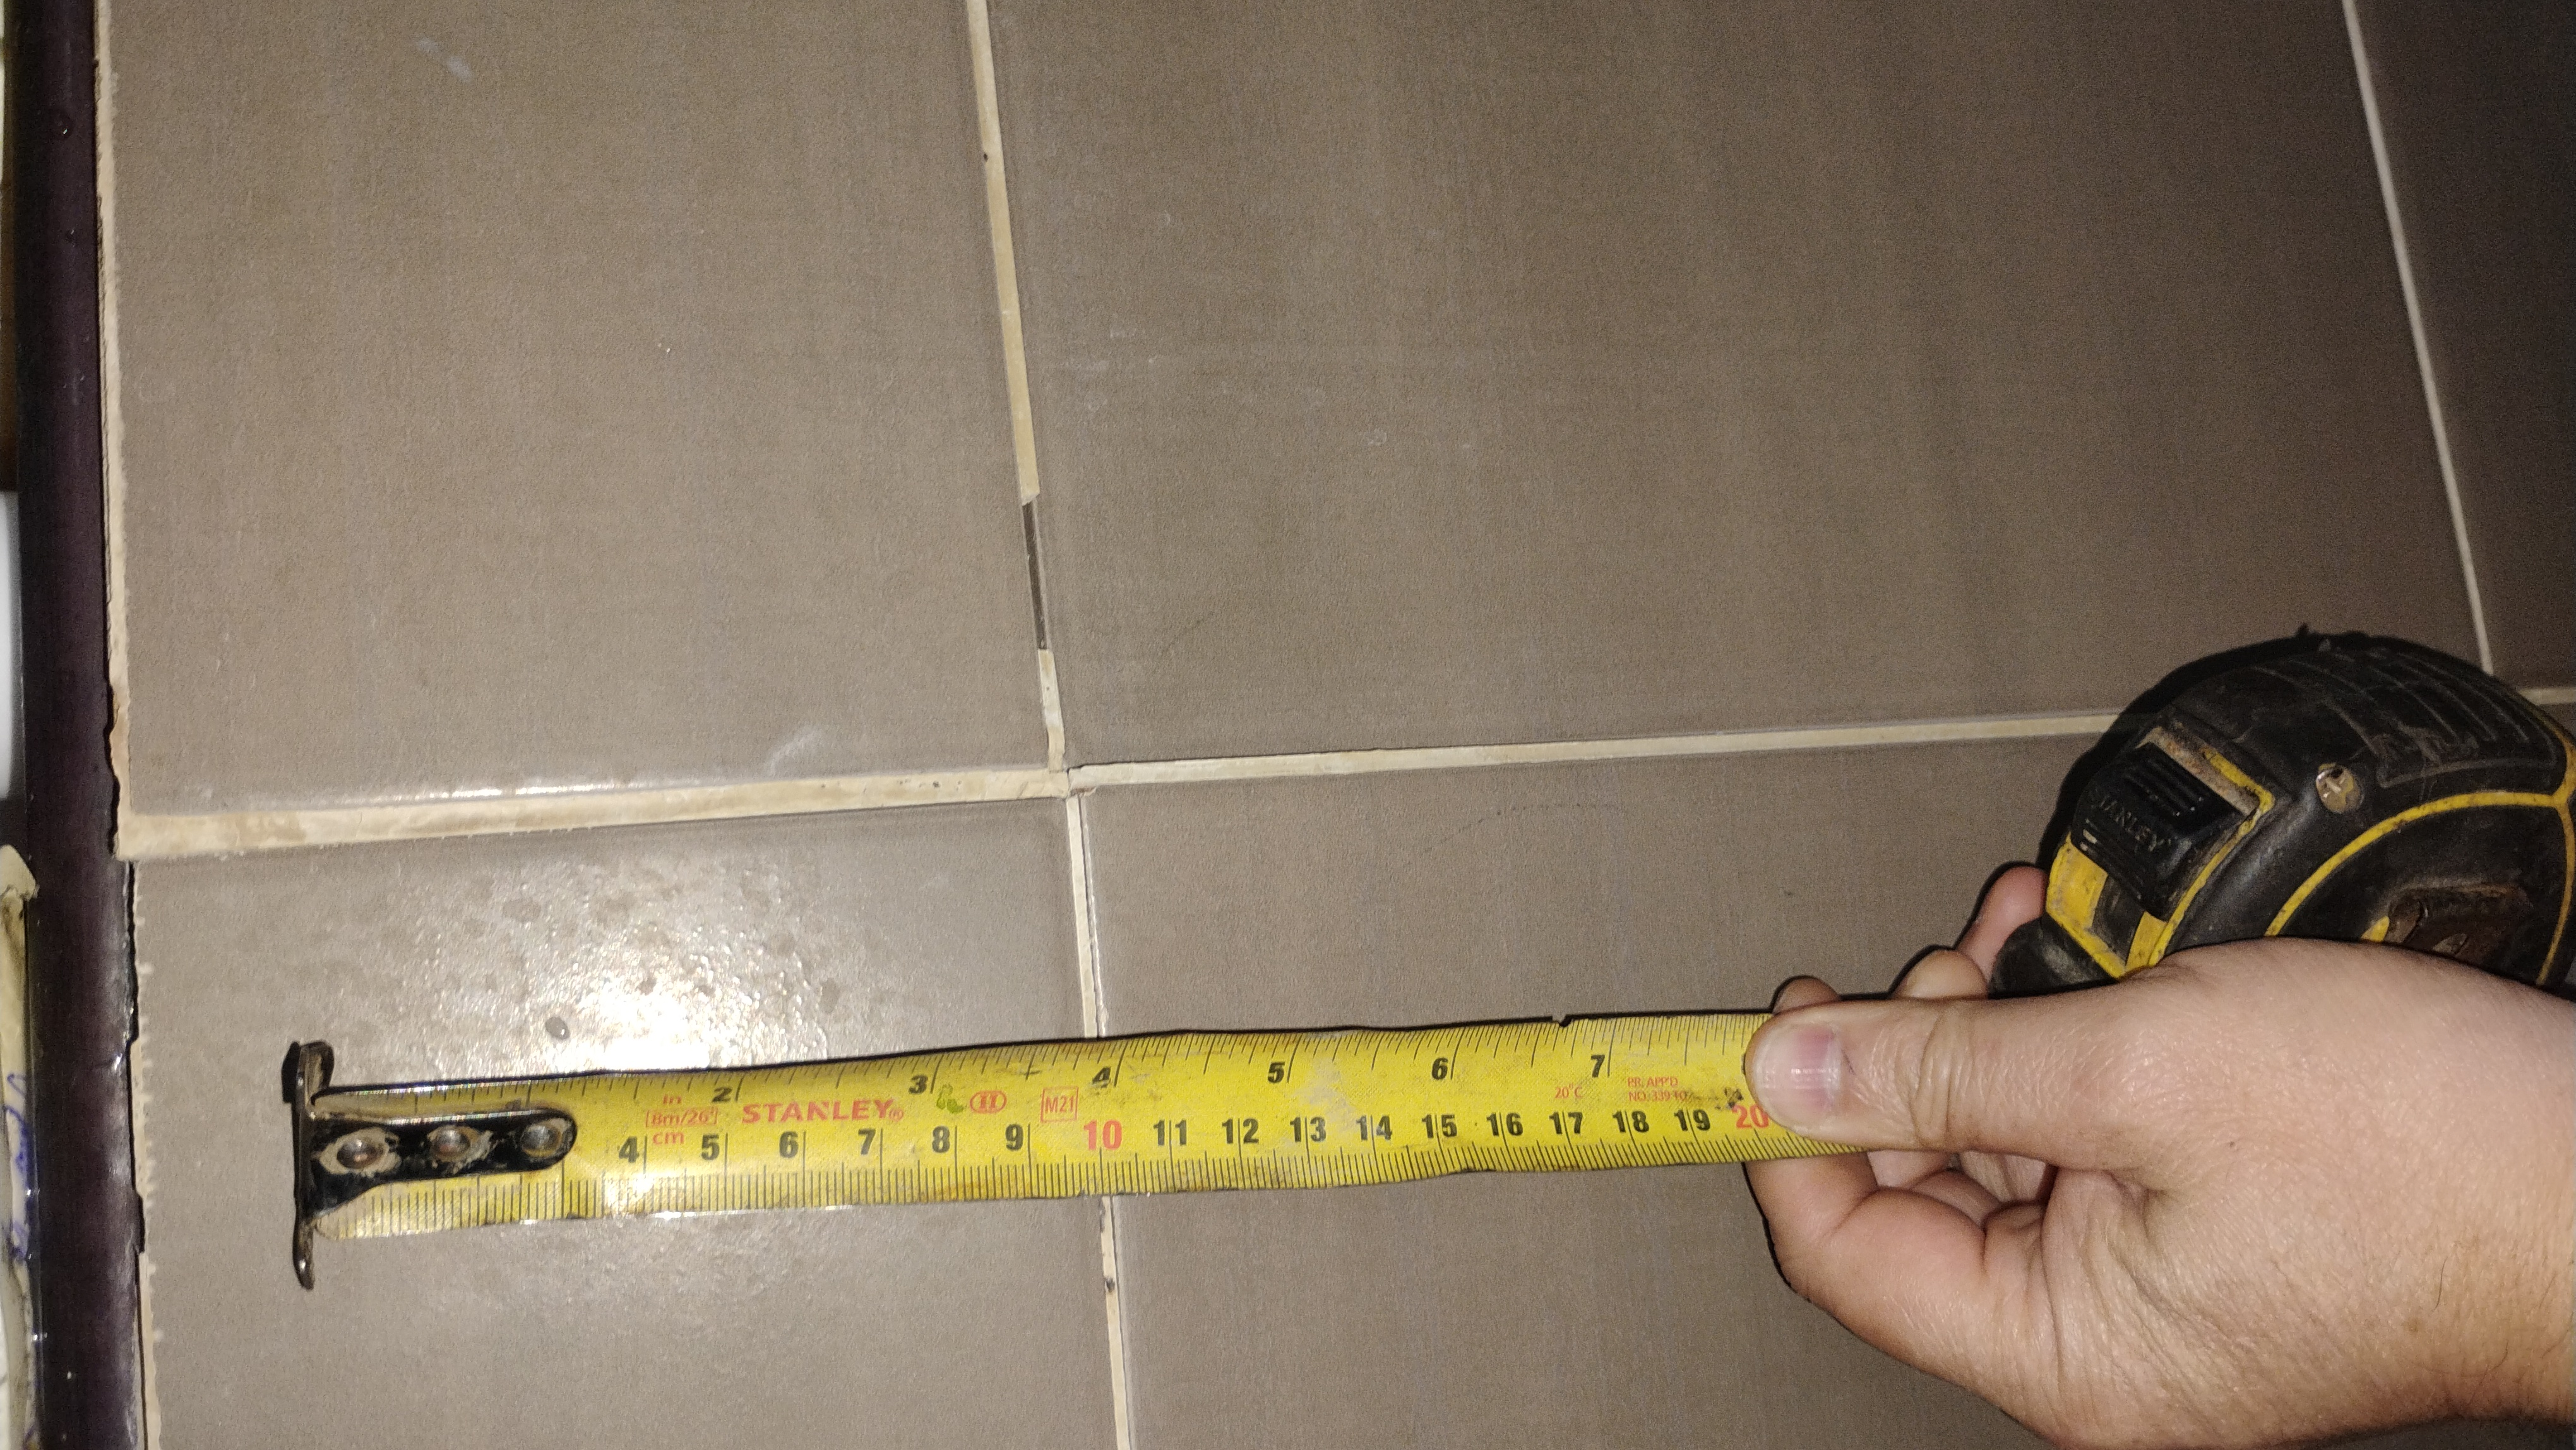
\includegraphics[width=\linewidth]{../img/IMG_20251109_151118514.jpg}\\[2pt]{\footnotesize\color{primary!60!black}Foto~16 -- 15:11:18}} \\[4pt]
\parbox{0.45\textwidth}{\centering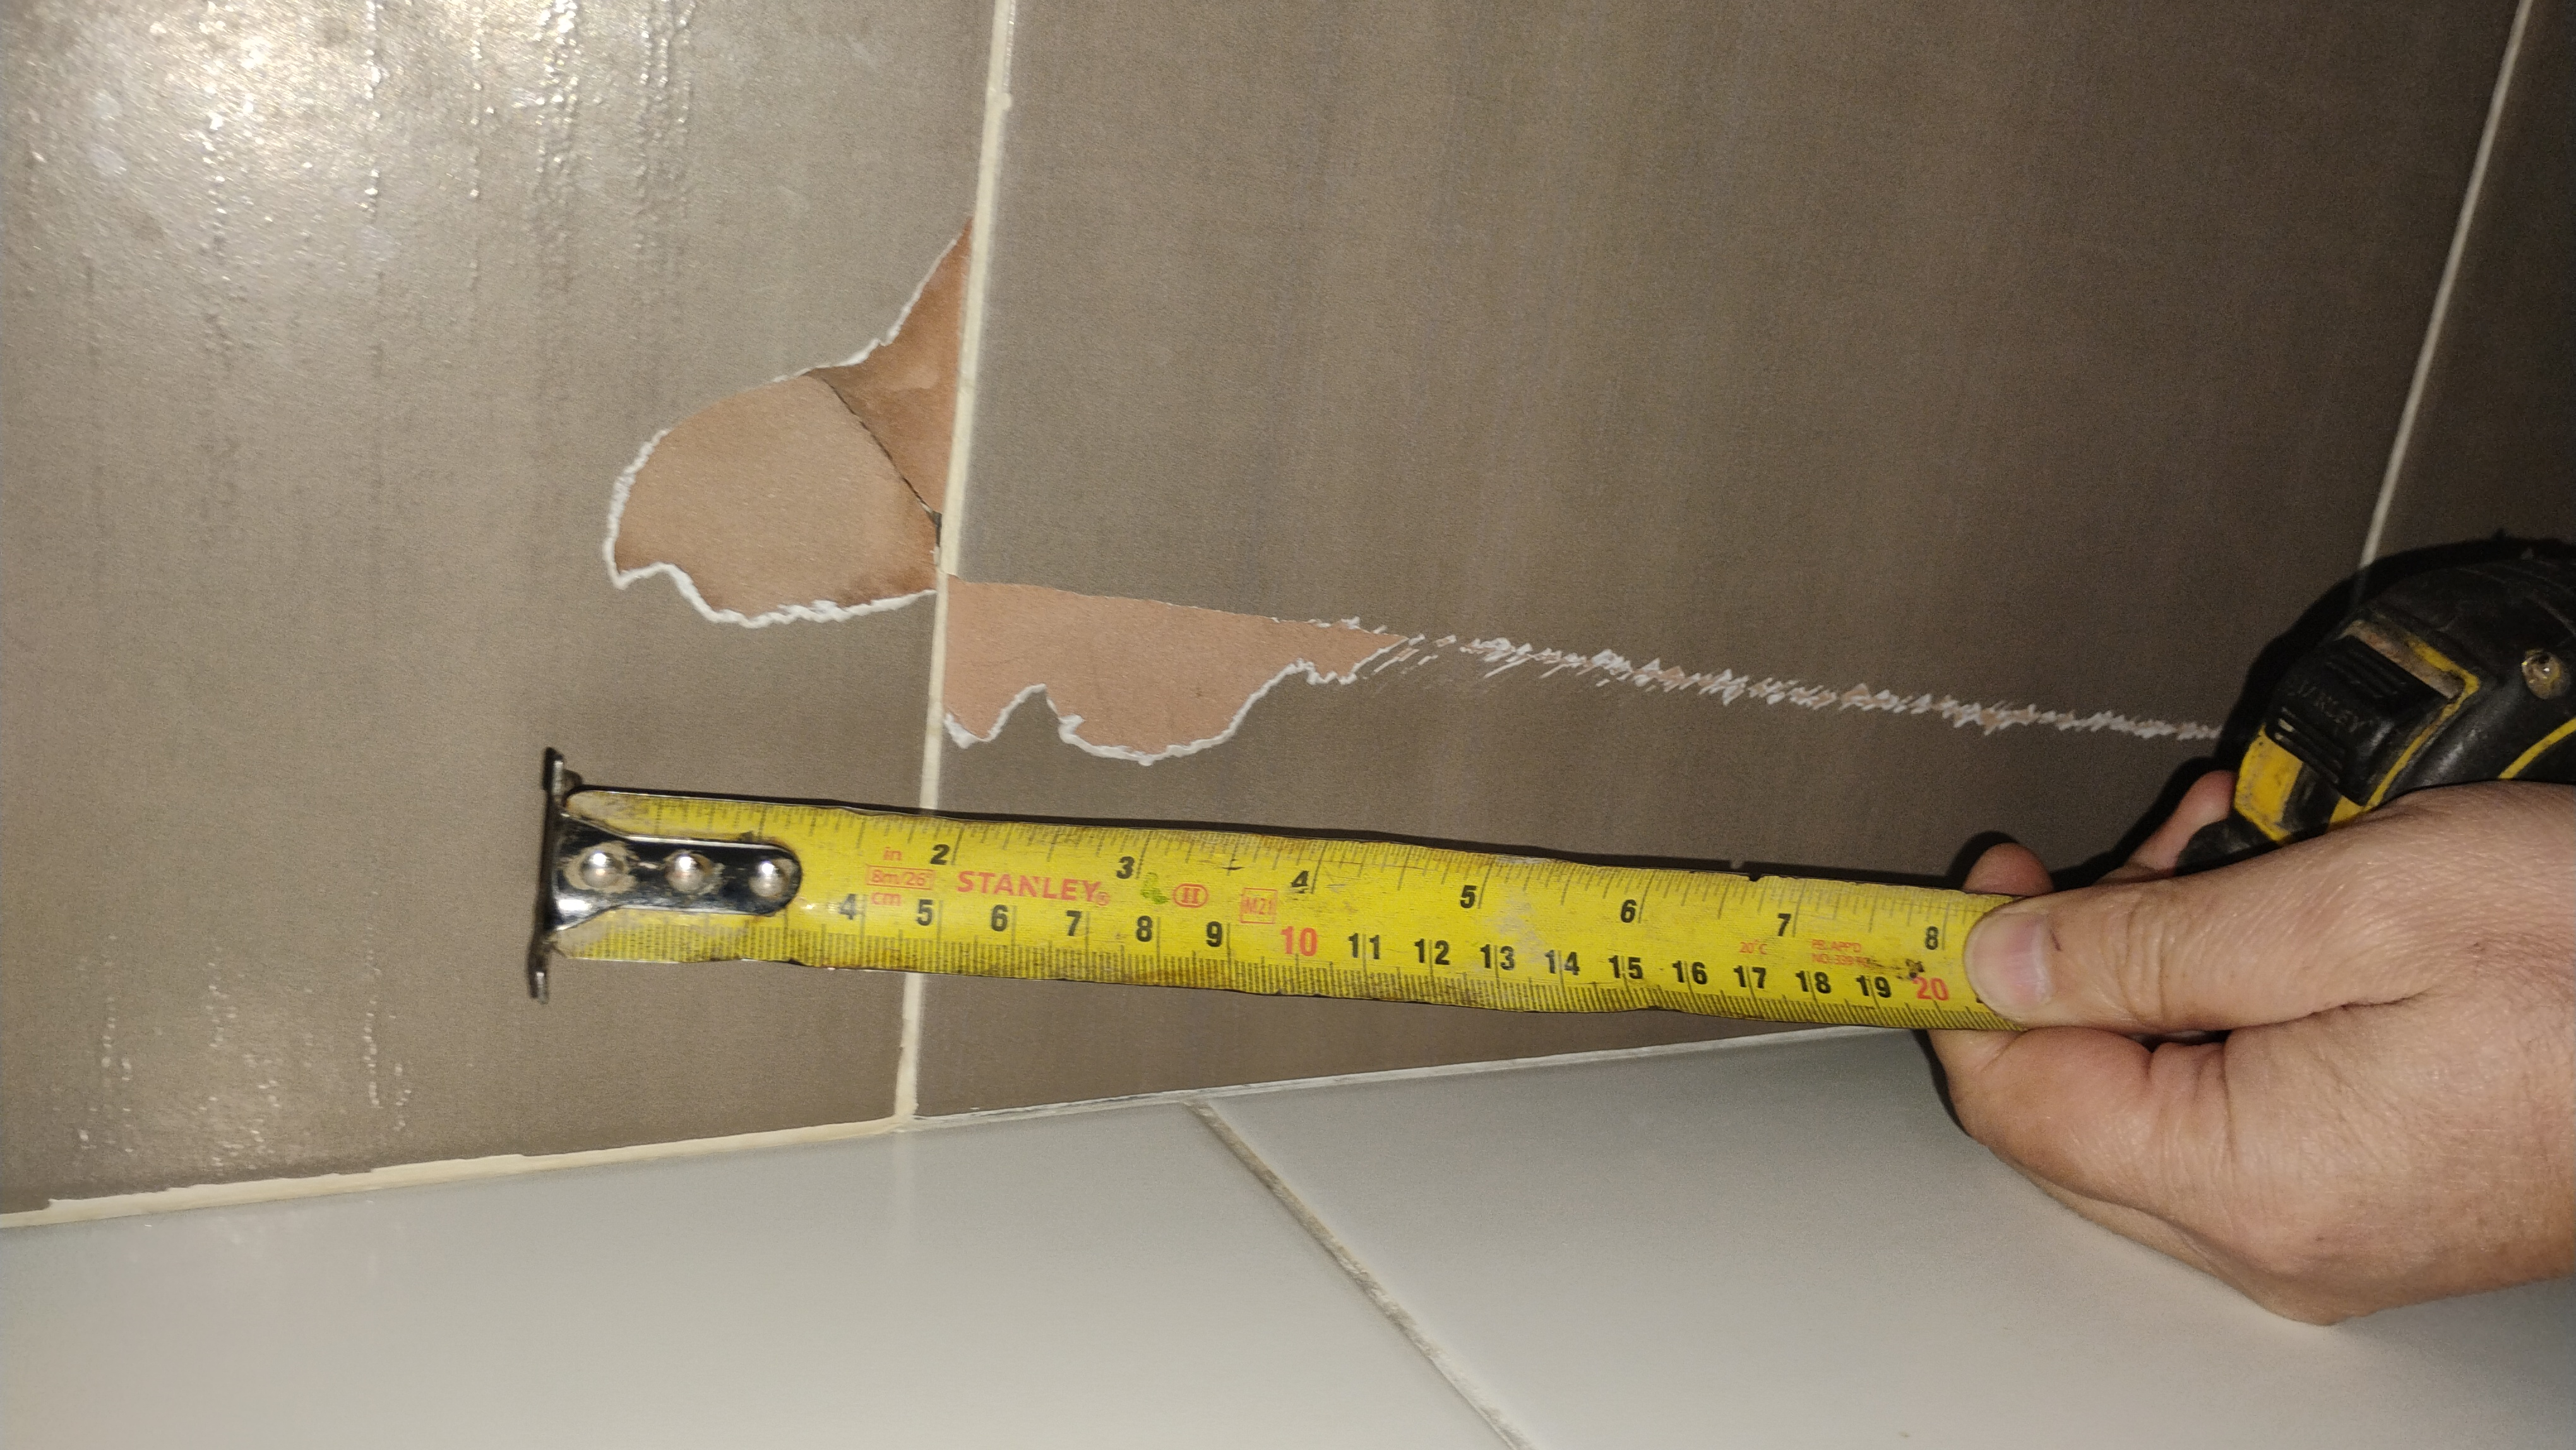
\includegraphics[width=\linewidth]{../img/IMG_20251109_151123725.jpg}\\[2pt]{\footnotesize\color{primary!60!black}Foto~17 -- 15:11:23}} & \parbox{0.45\textwidth}{\centering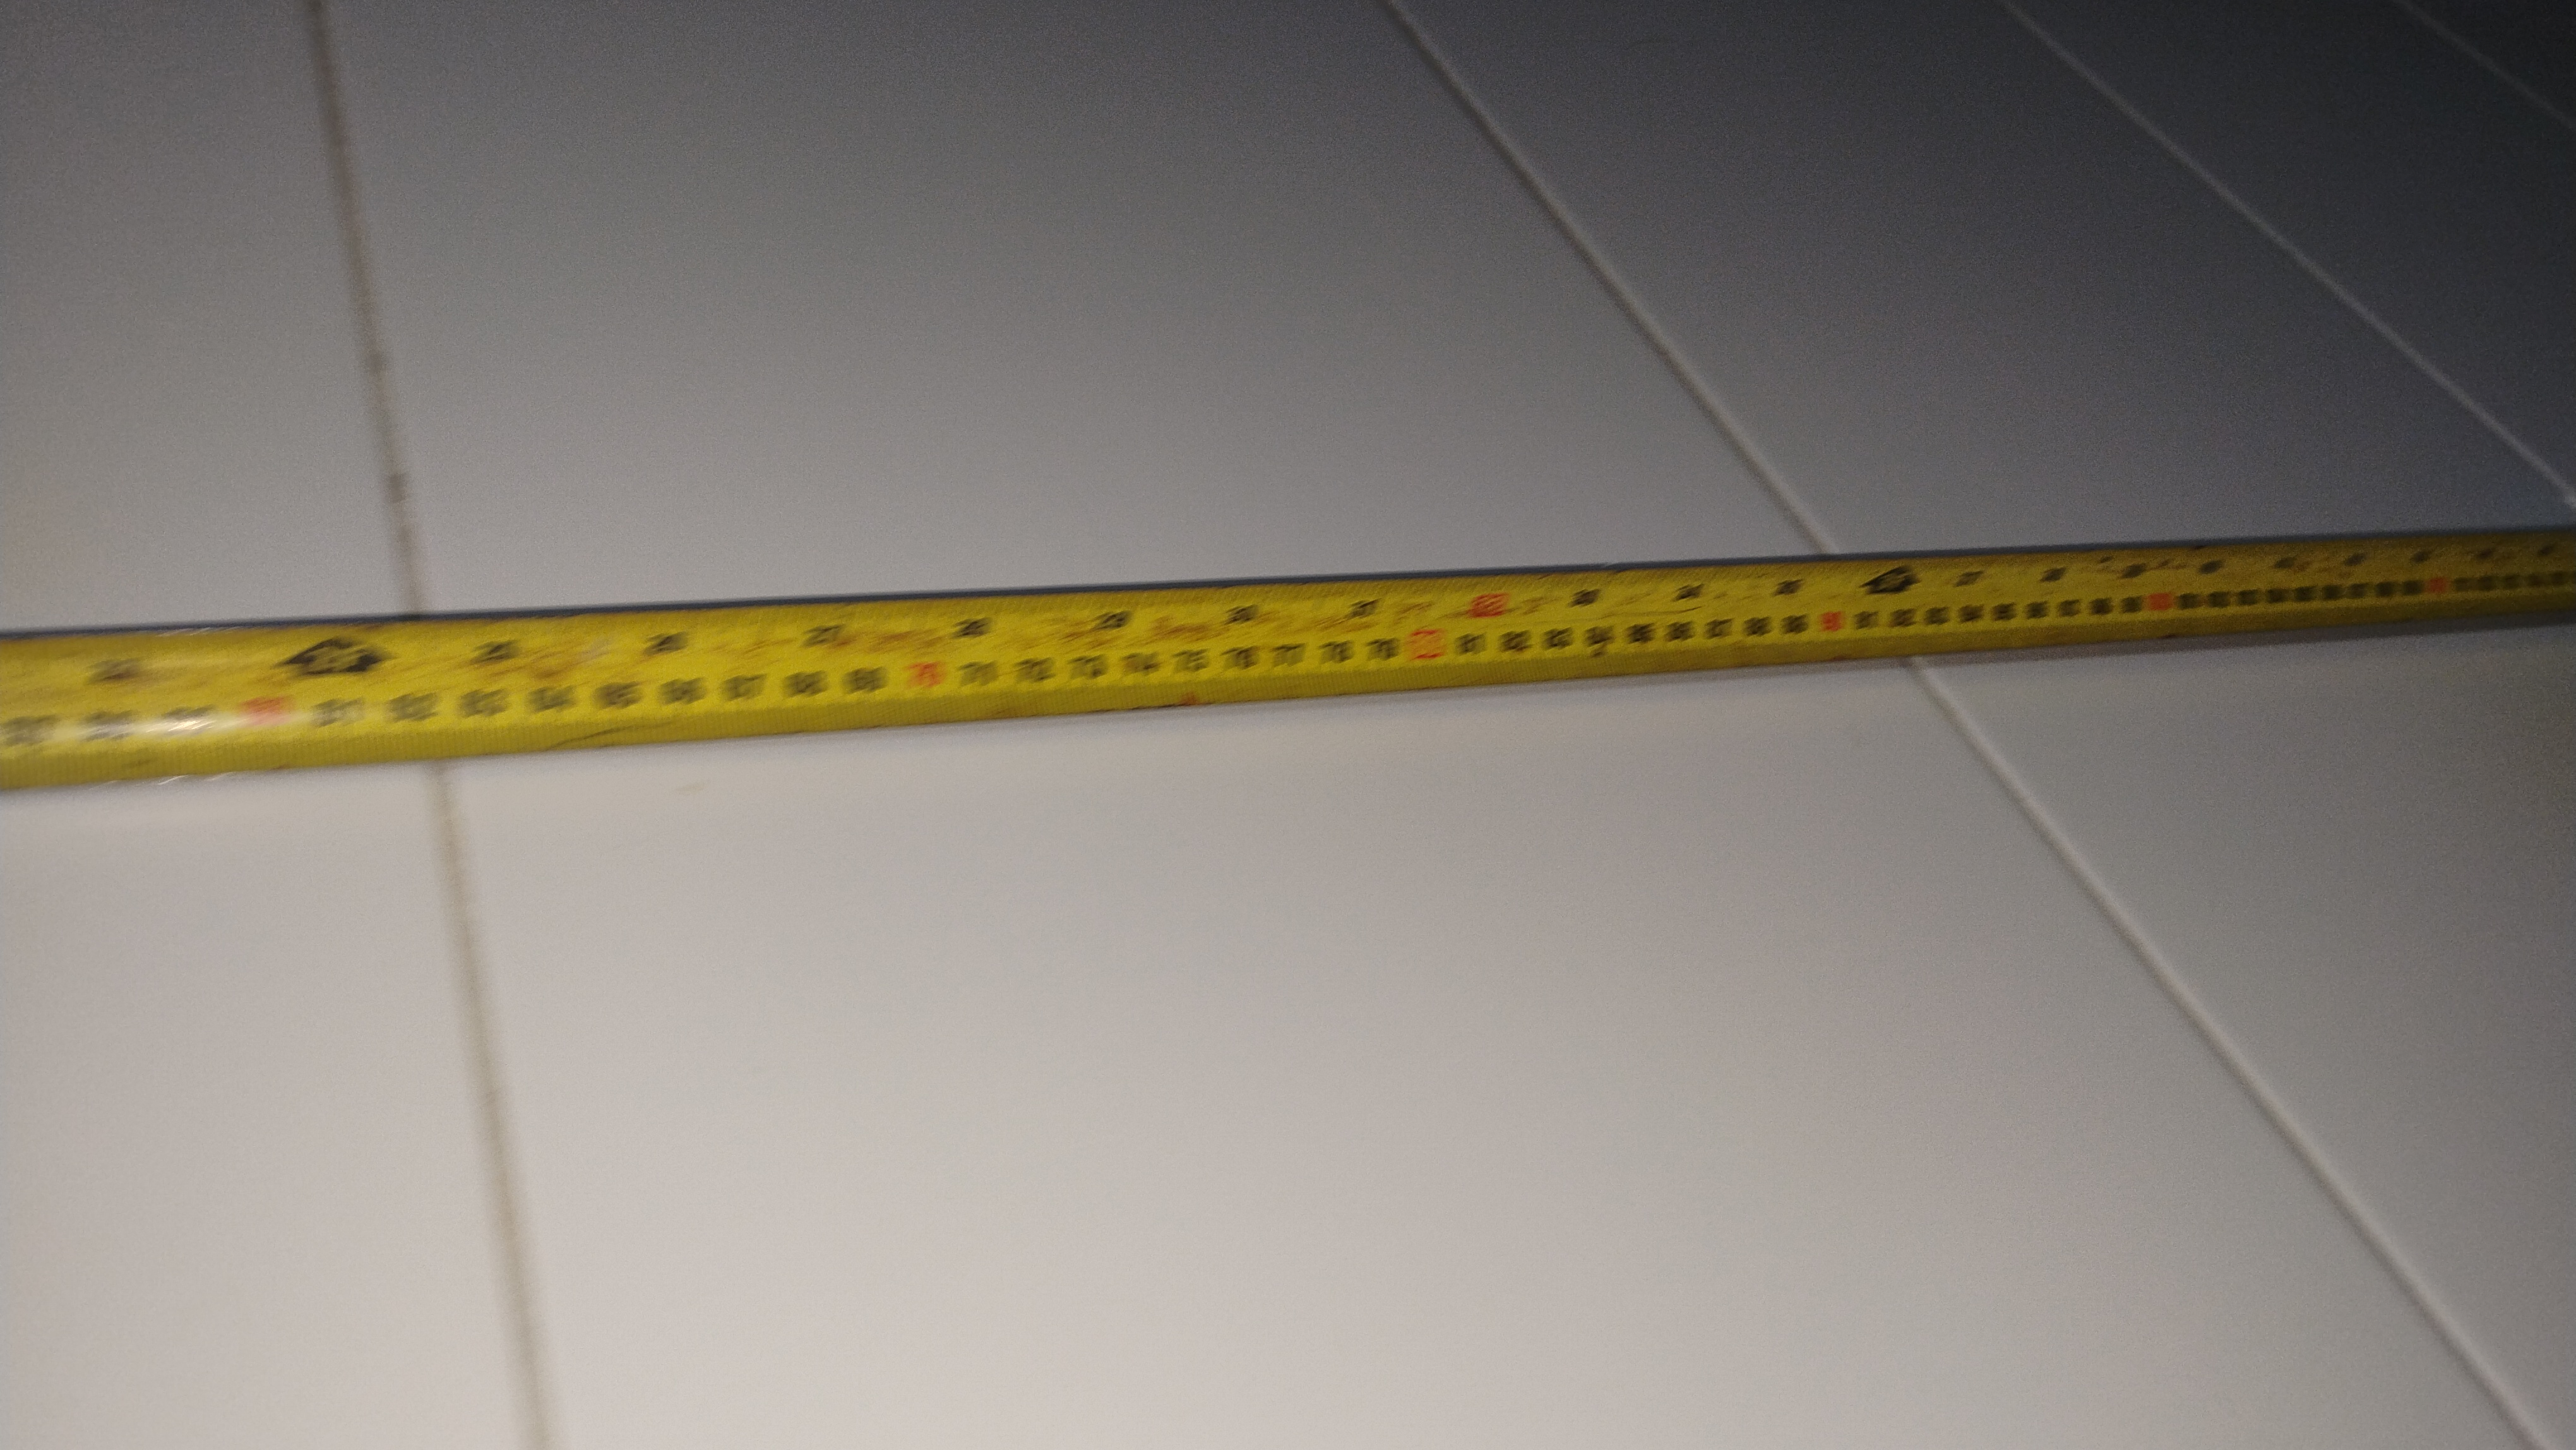
\includegraphics[width=\linewidth]{../img/IMG_20251109_151214900.jpg}\\[2pt]{\footnotesize\color{primary!60!black}Foto~18 -- 15:12:14}} \\[4pt]
\end{tabular}
\caption{Zócalo y Paramento Sur — Humedad por Capilaridad y Eflorescencia: Fotos 13 al 18.}\end{figure}
\newpage
\begin{figure}[H]
\centering
\begin{tabular}{cc}
\parbox{0.45\textwidth}{\centering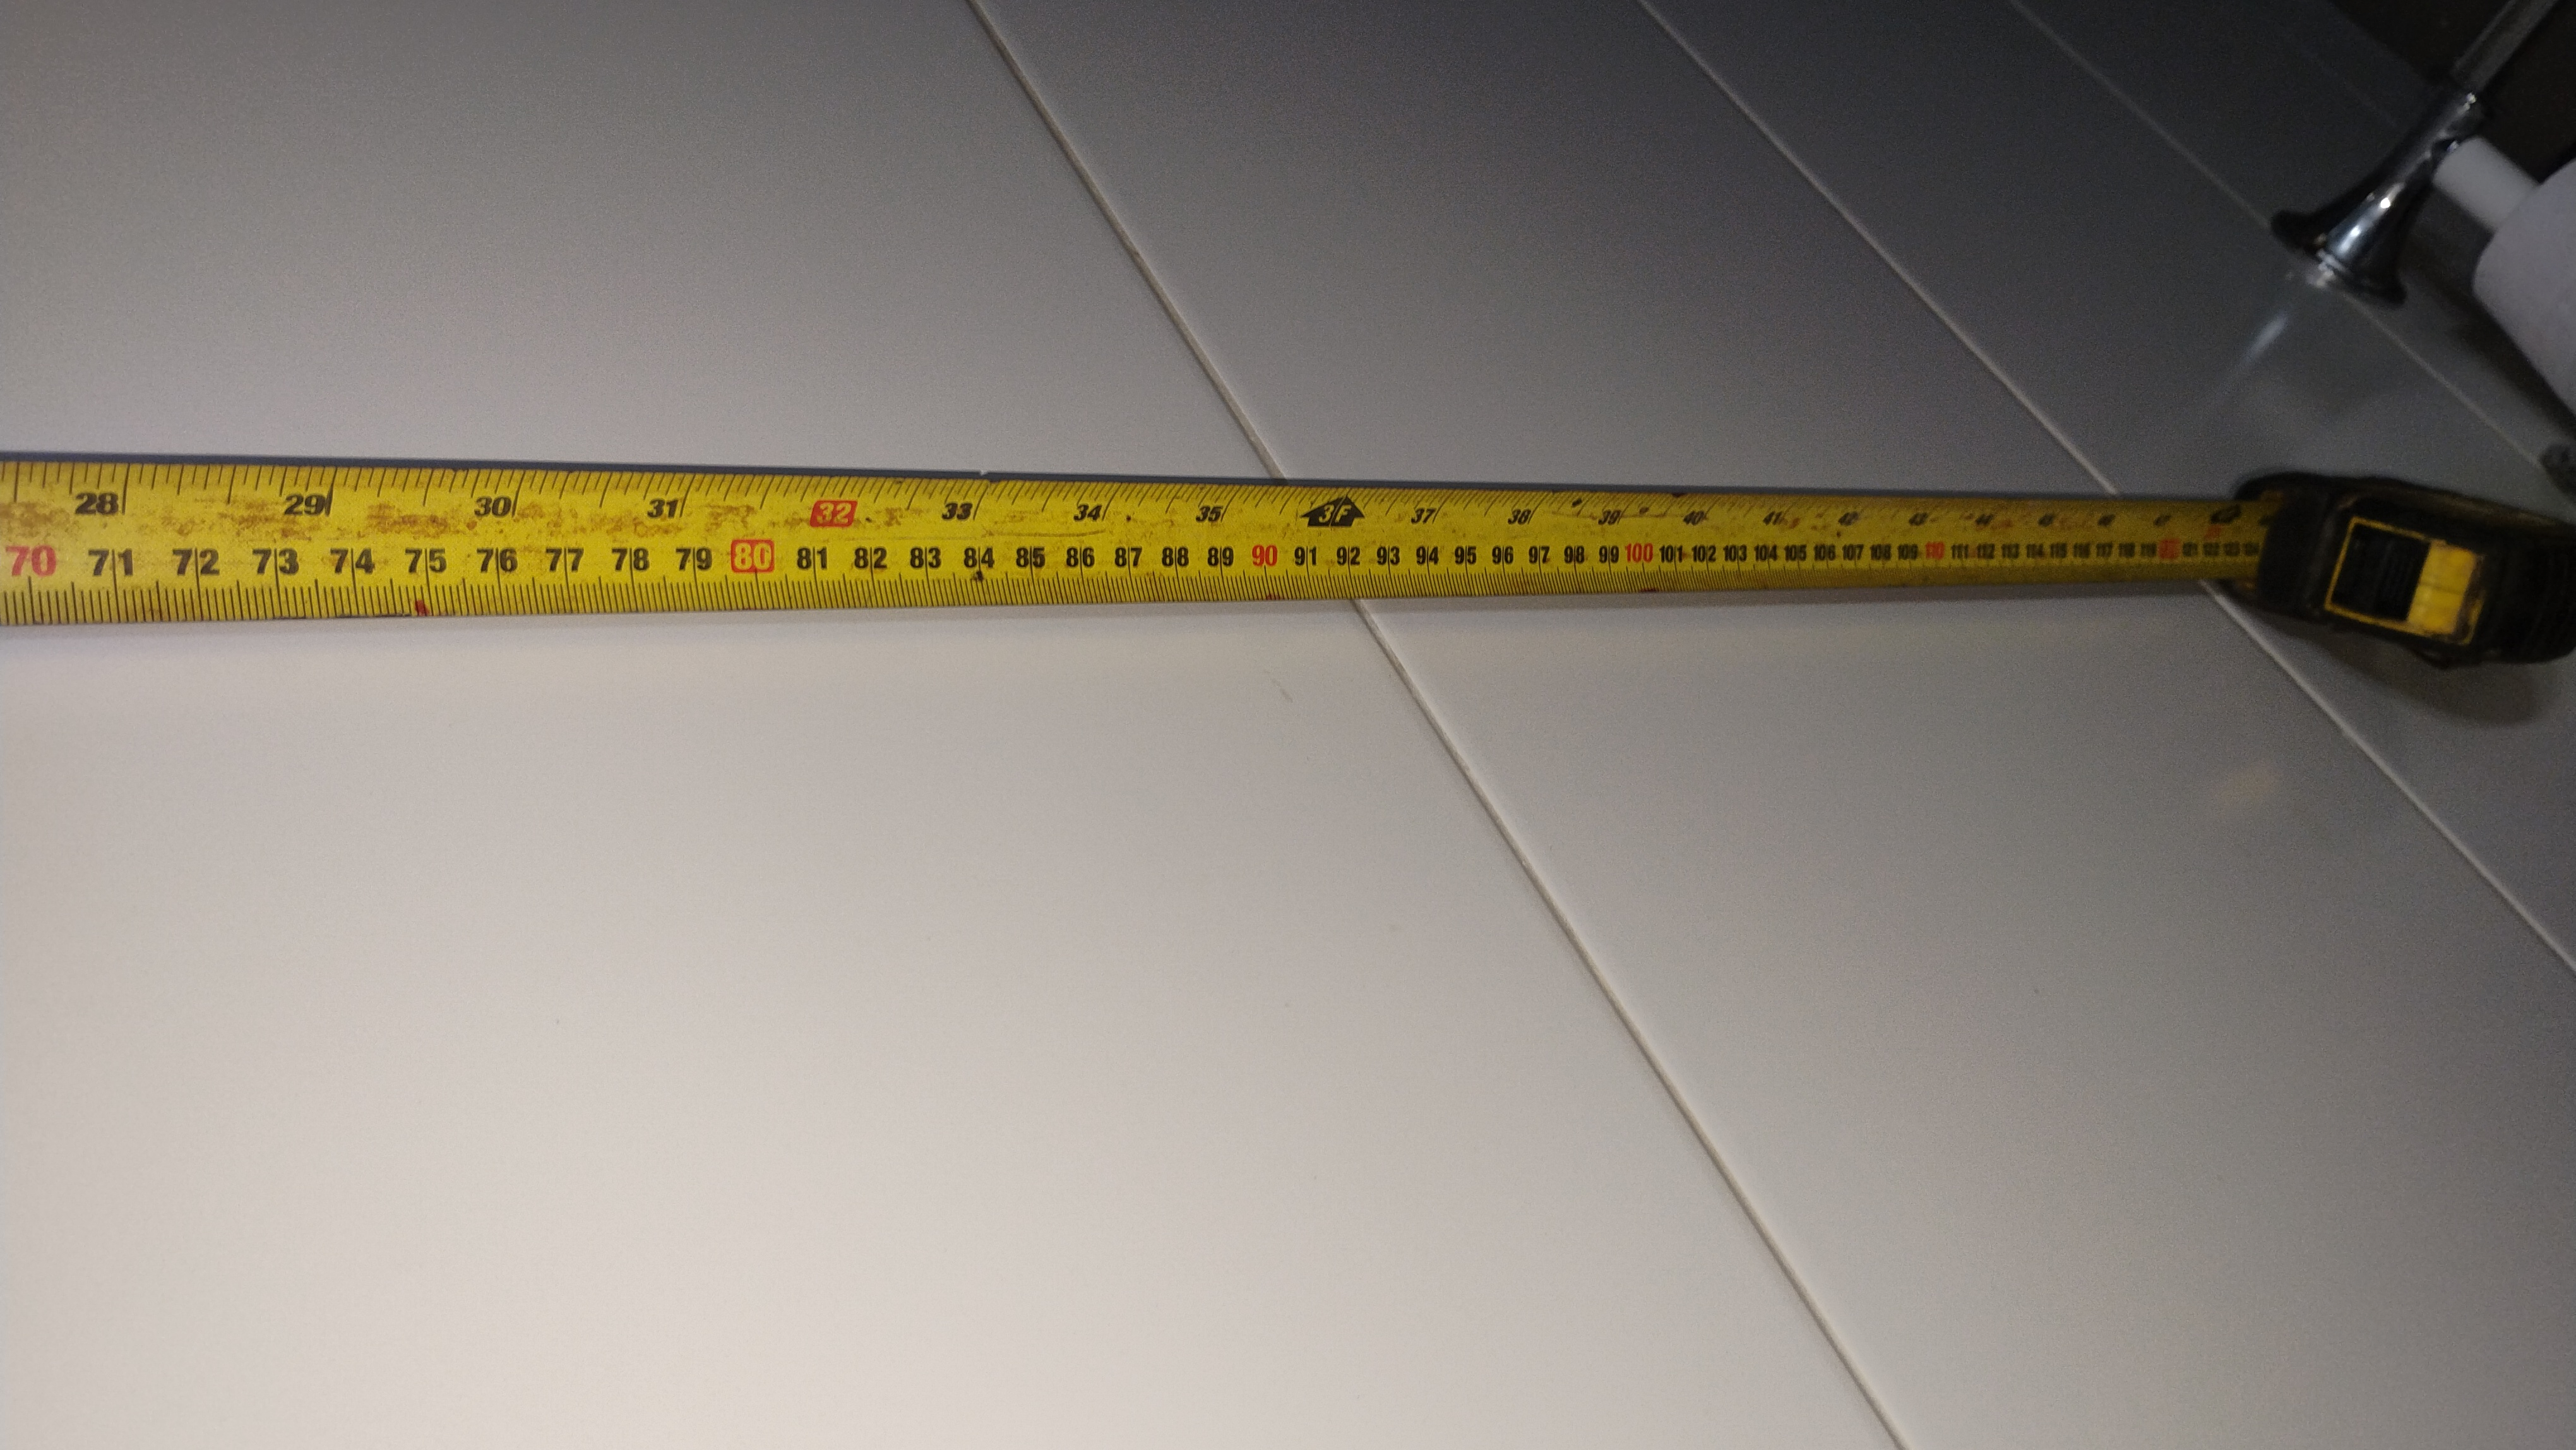
\includegraphics[width=\linewidth]{../img/IMG_20251109_151217765.jpg}\\[2pt]{\footnotesize\color{primary!60!black}Foto~19 -- 15:12:17}} & \parbox{0.45\textwidth}{\centering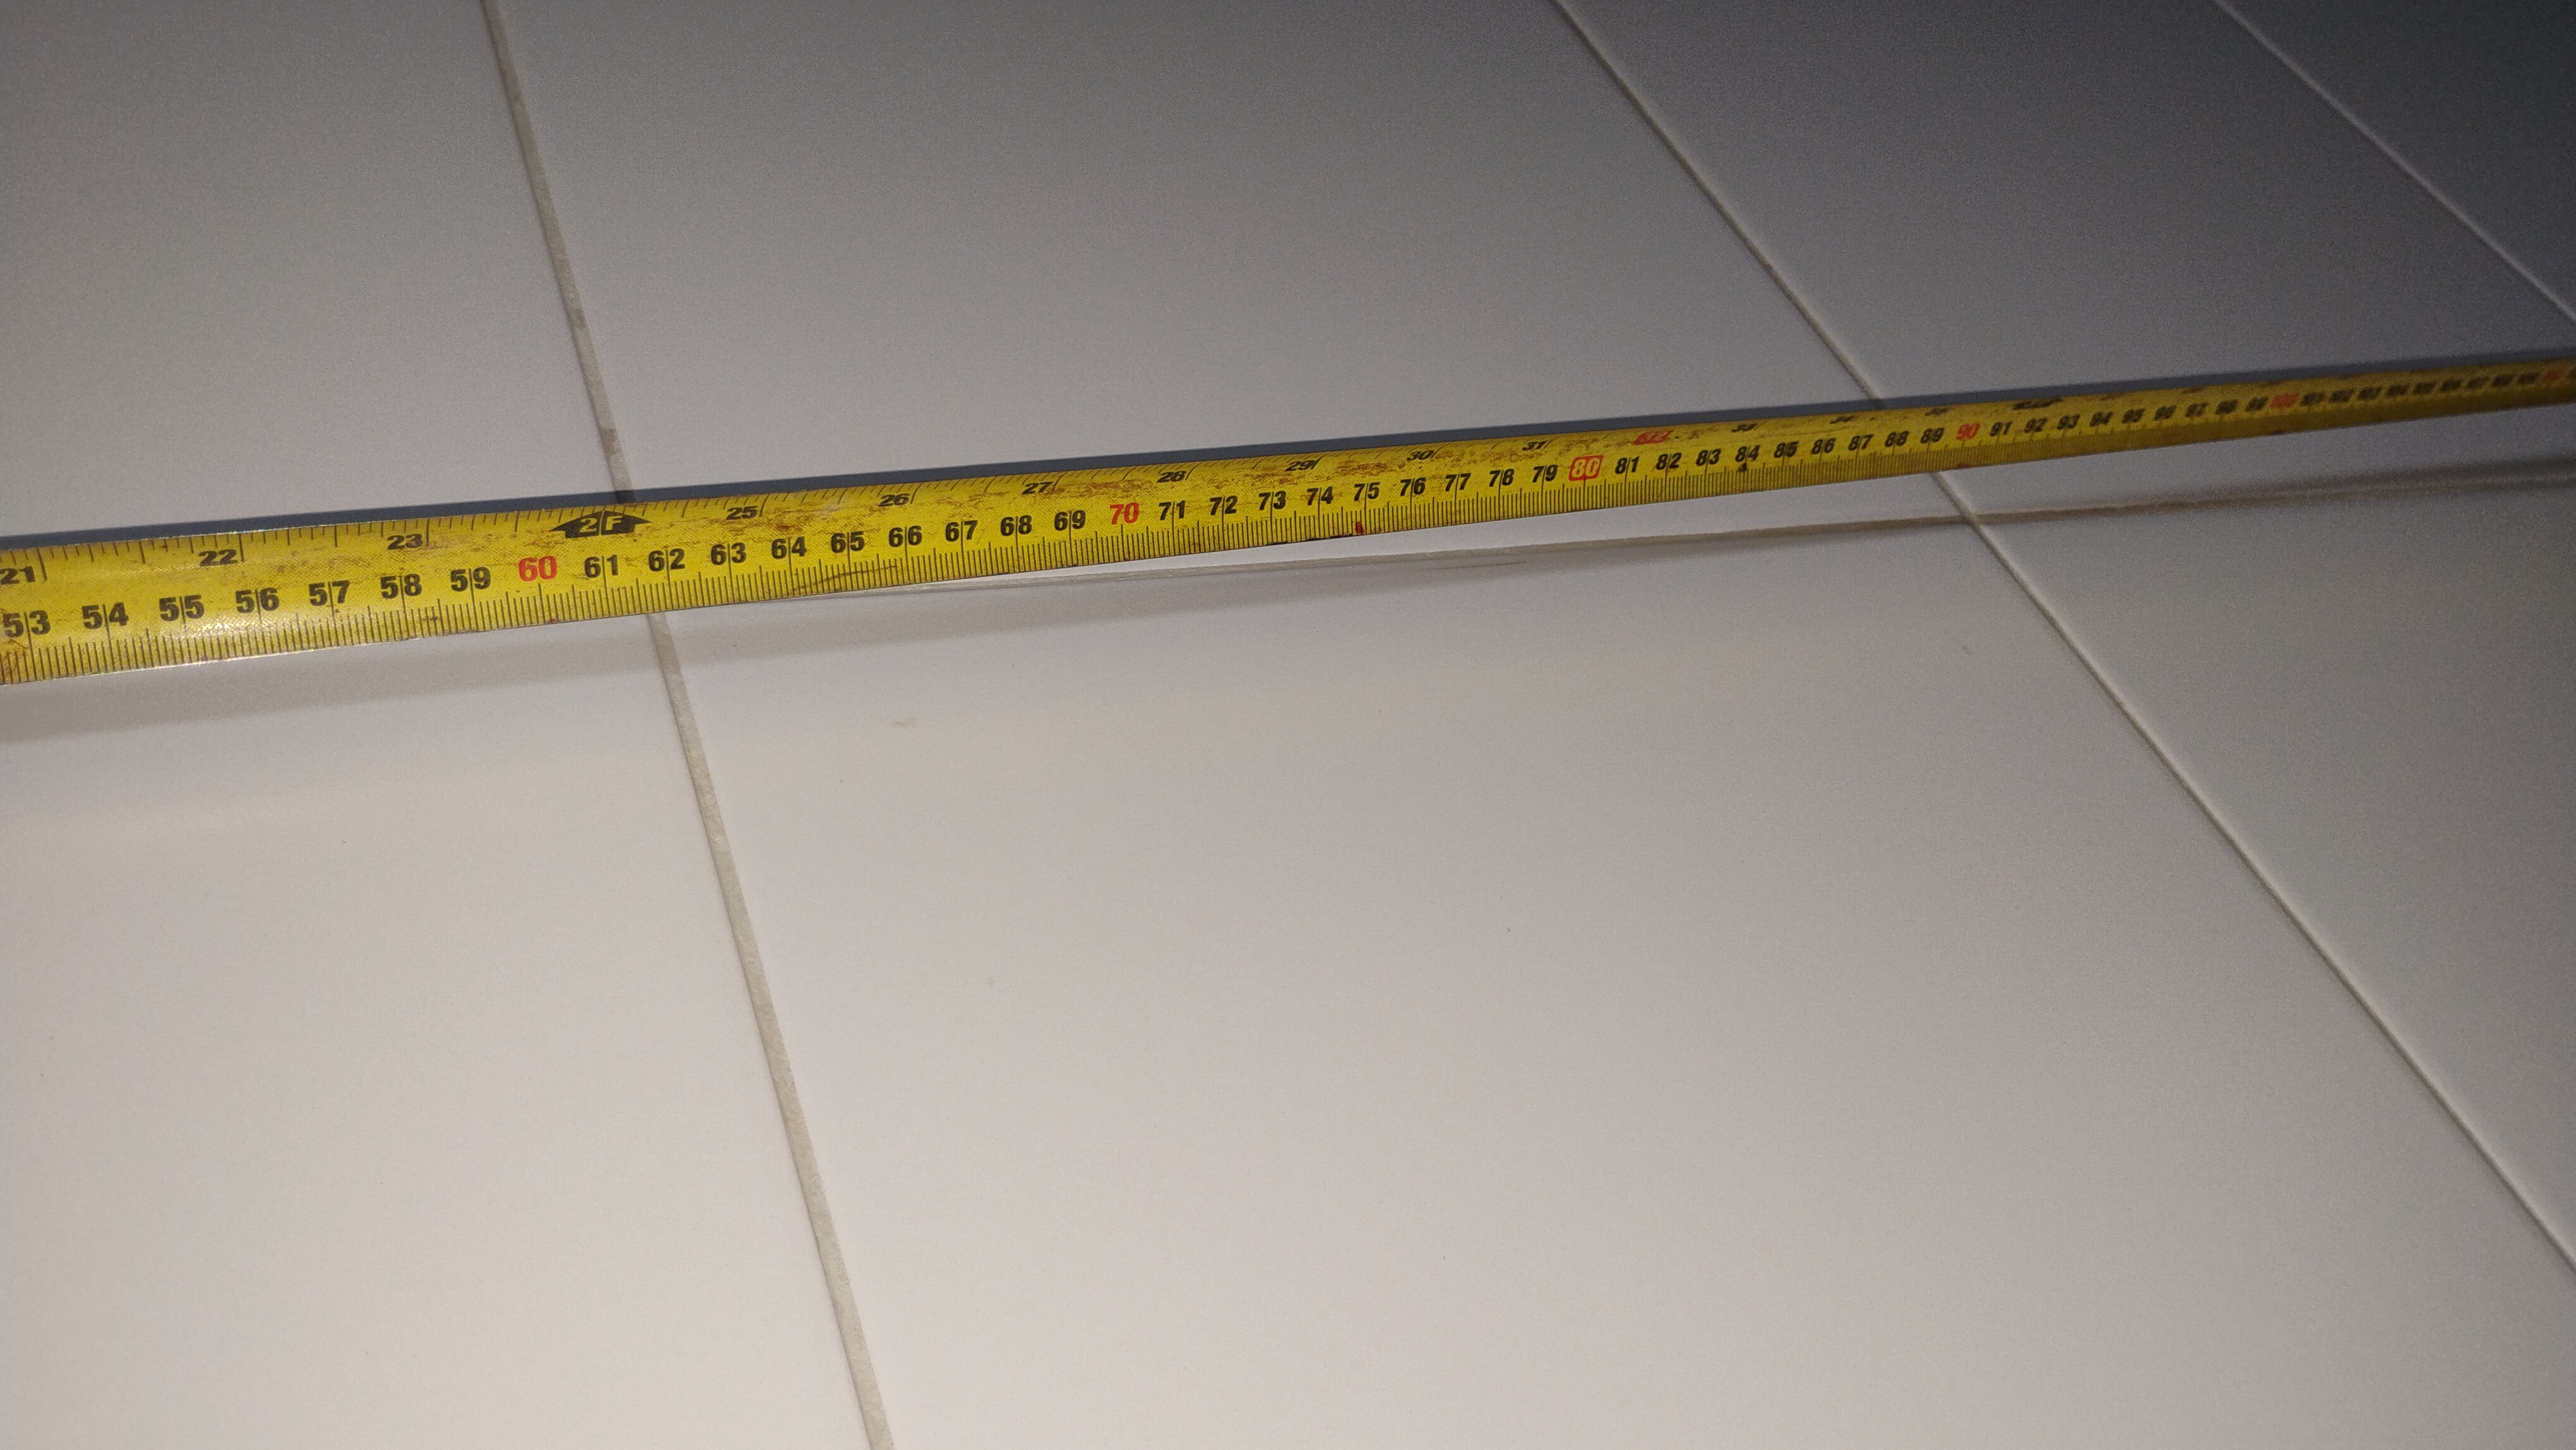
\includegraphics[width=\linewidth]{../img/IMG_20251109_151223989.jpg}\\[2pt]{\footnotesize\color{primary!60!black}Foto~20 -- 15:12:23}} \\[4pt]
\parbox{0.45\textwidth}{\centering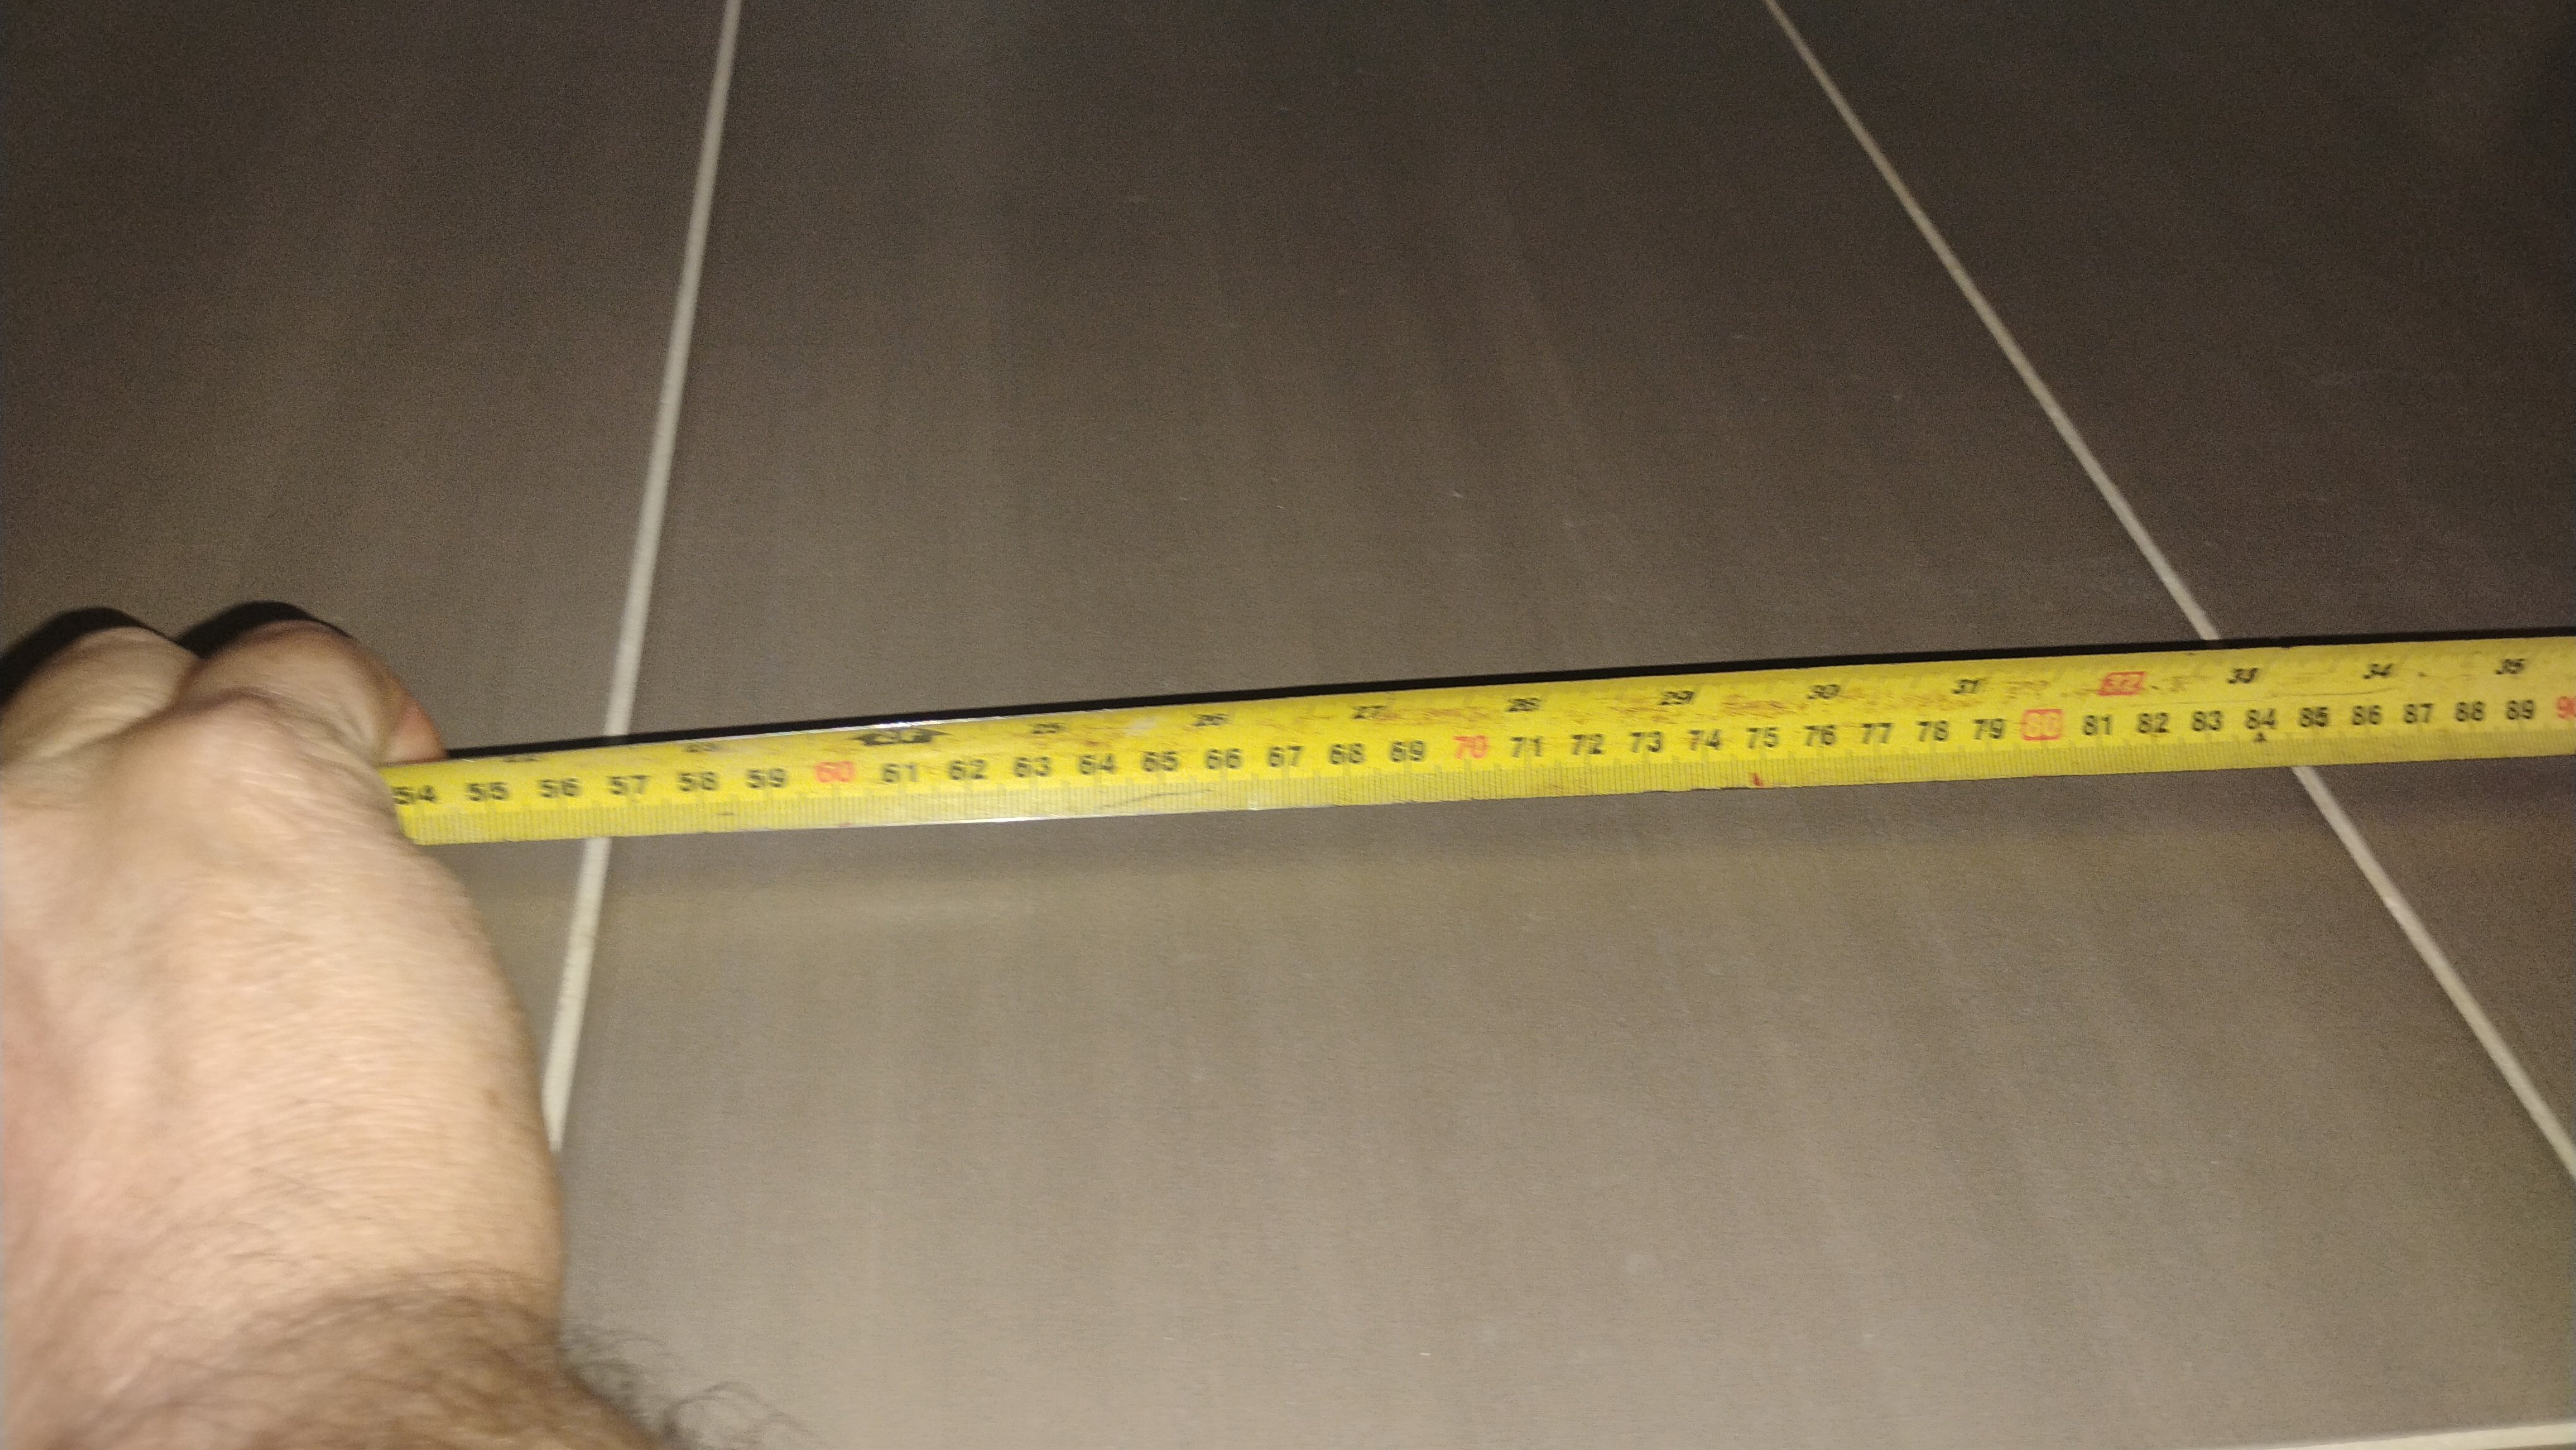
\includegraphics[width=\linewidth]{../img/IMG_20251109_151318648.jpg}\\[2pt]{\footnotesize\color{primary!60!black}Foto~21 -- 15:13:18}} & \parbox{0.45\textwidth}{\centering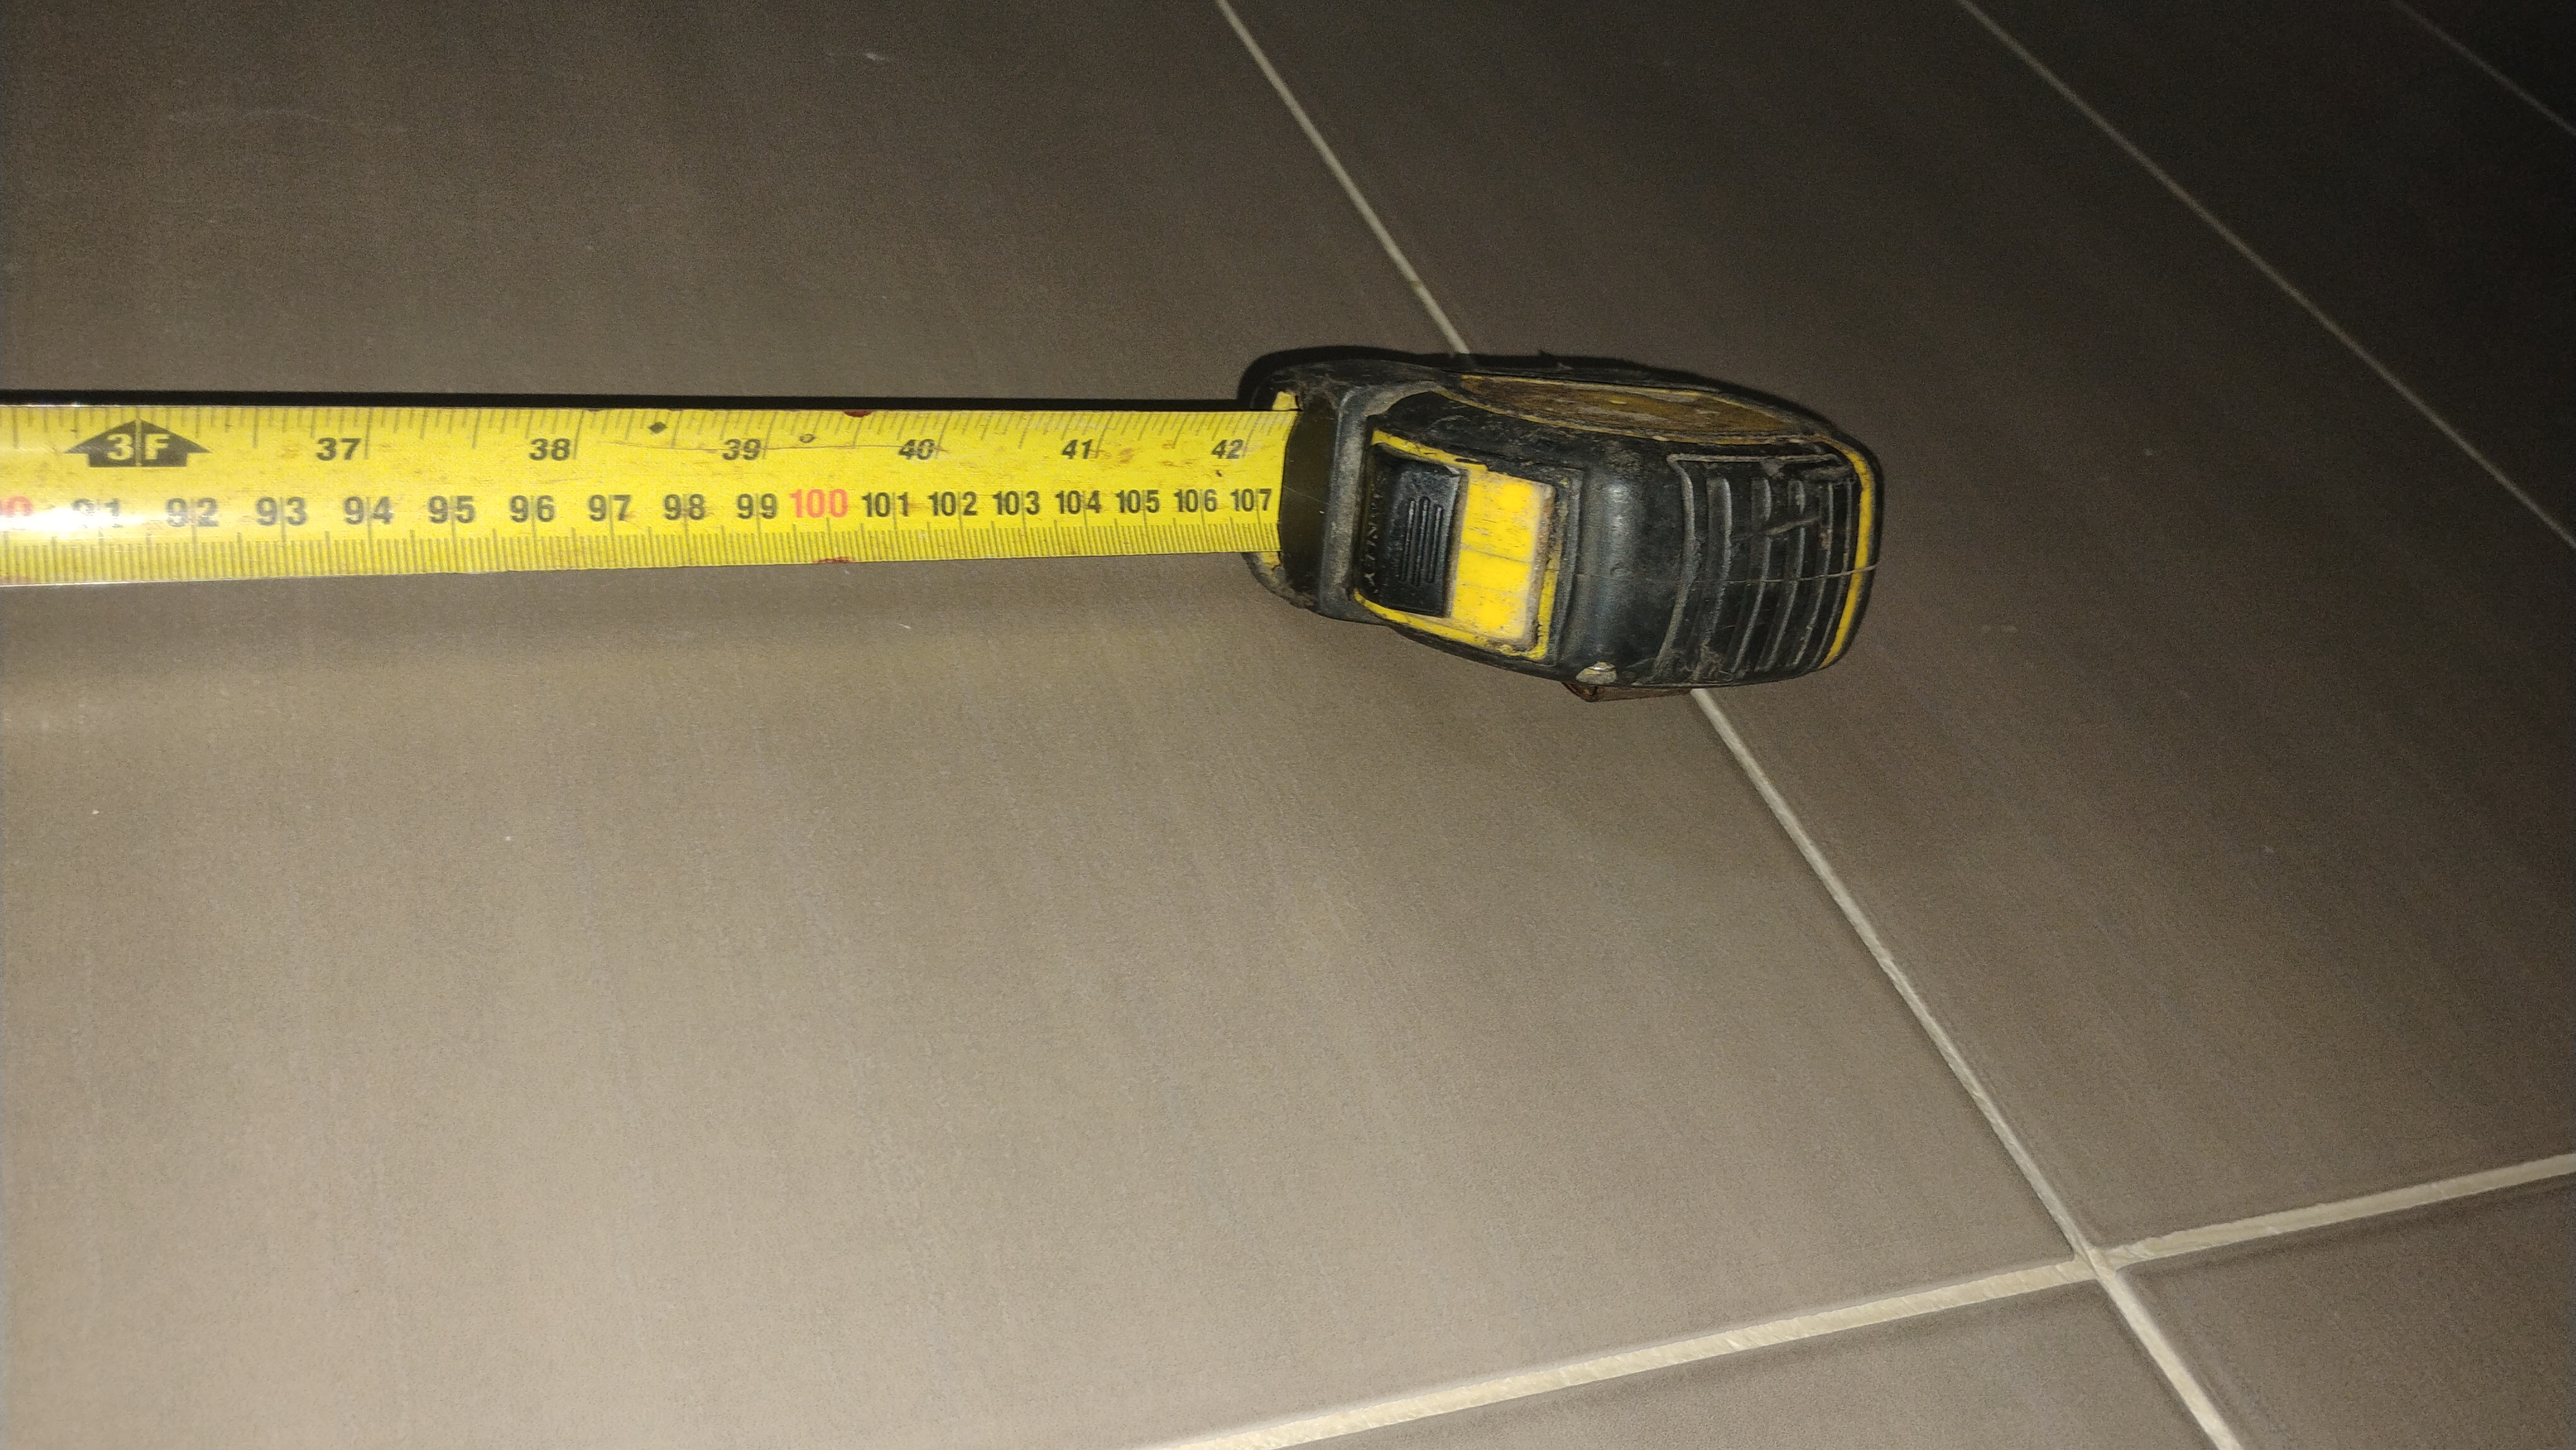
\includegraphics[width=\linewidth]{../img/IMG_20251109_151325252.jpg}\\[2pt]{\footnotesize\color{primary!60!black}Foto~22 -- 15:13:25}} \\[4pt]
\parbox{0.45\textwidth}{\centering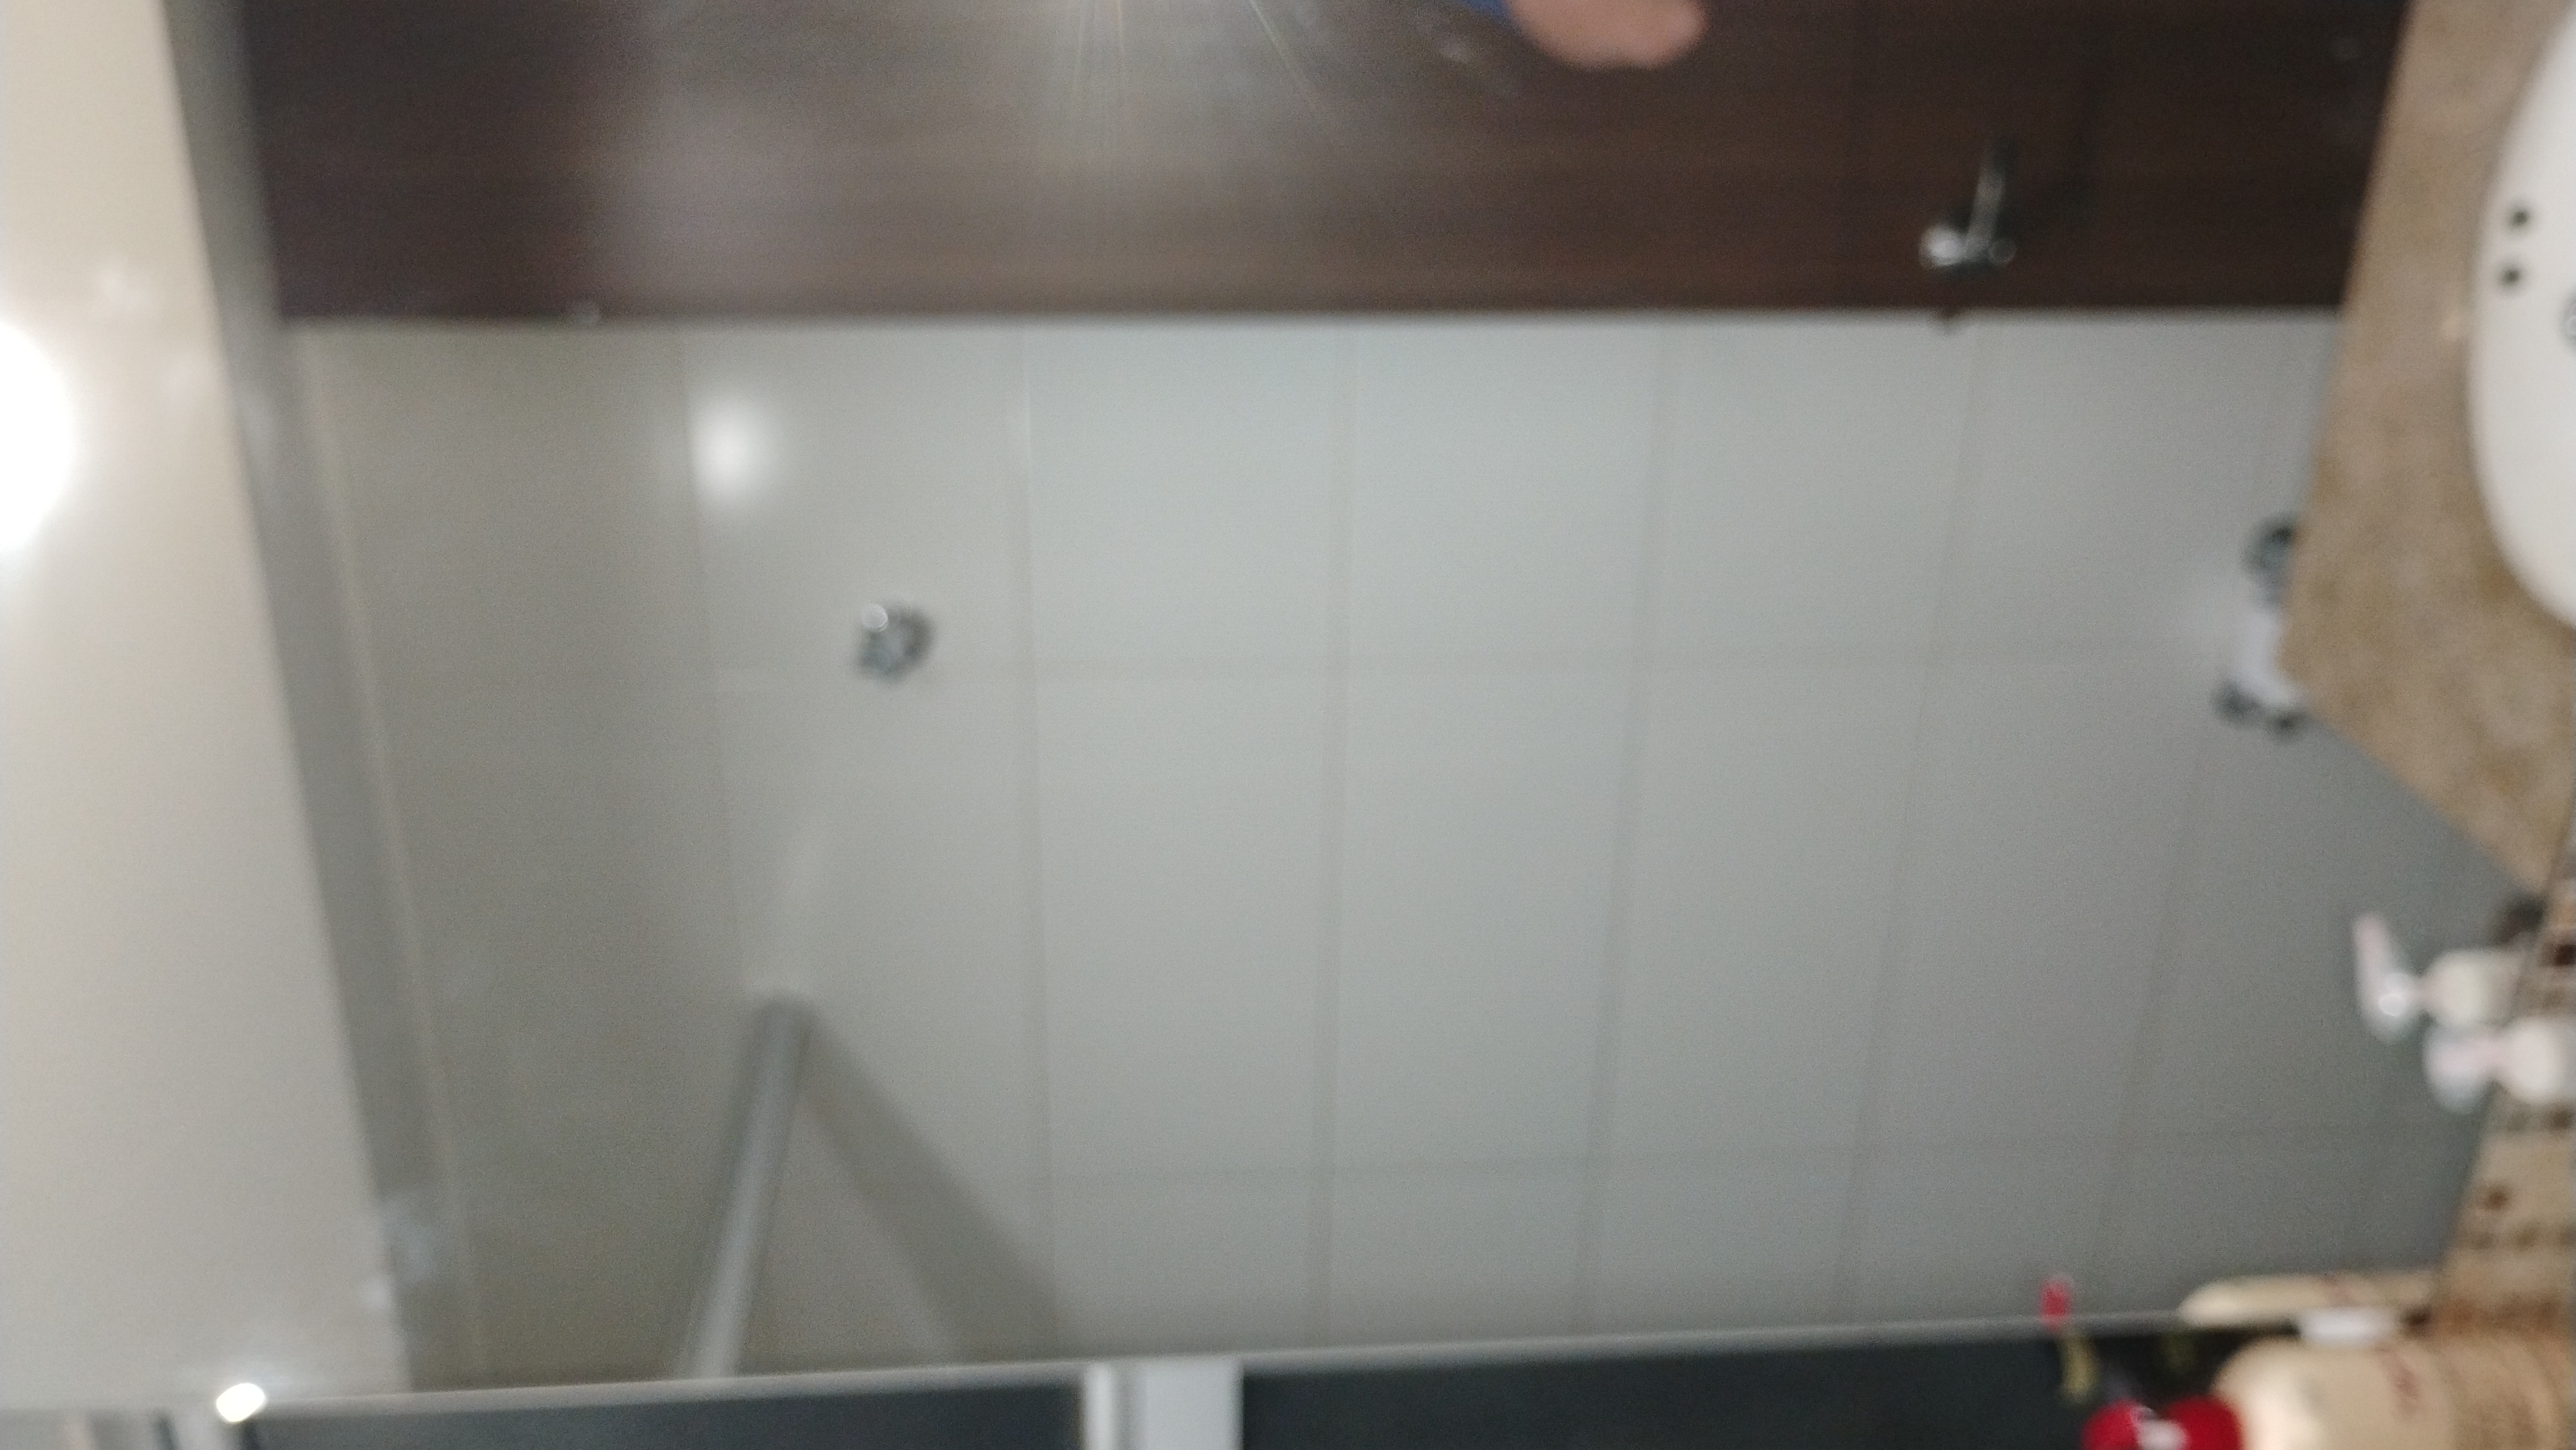
\includegraphics[width=\linewidth]{../img/IMG_20251109_151511756.jpg}\\[2pt]{\footnotesize\color{primary!60!black}Foto~23 -- 15:15:11}} & \parbox{0.45\textwidth}{\centering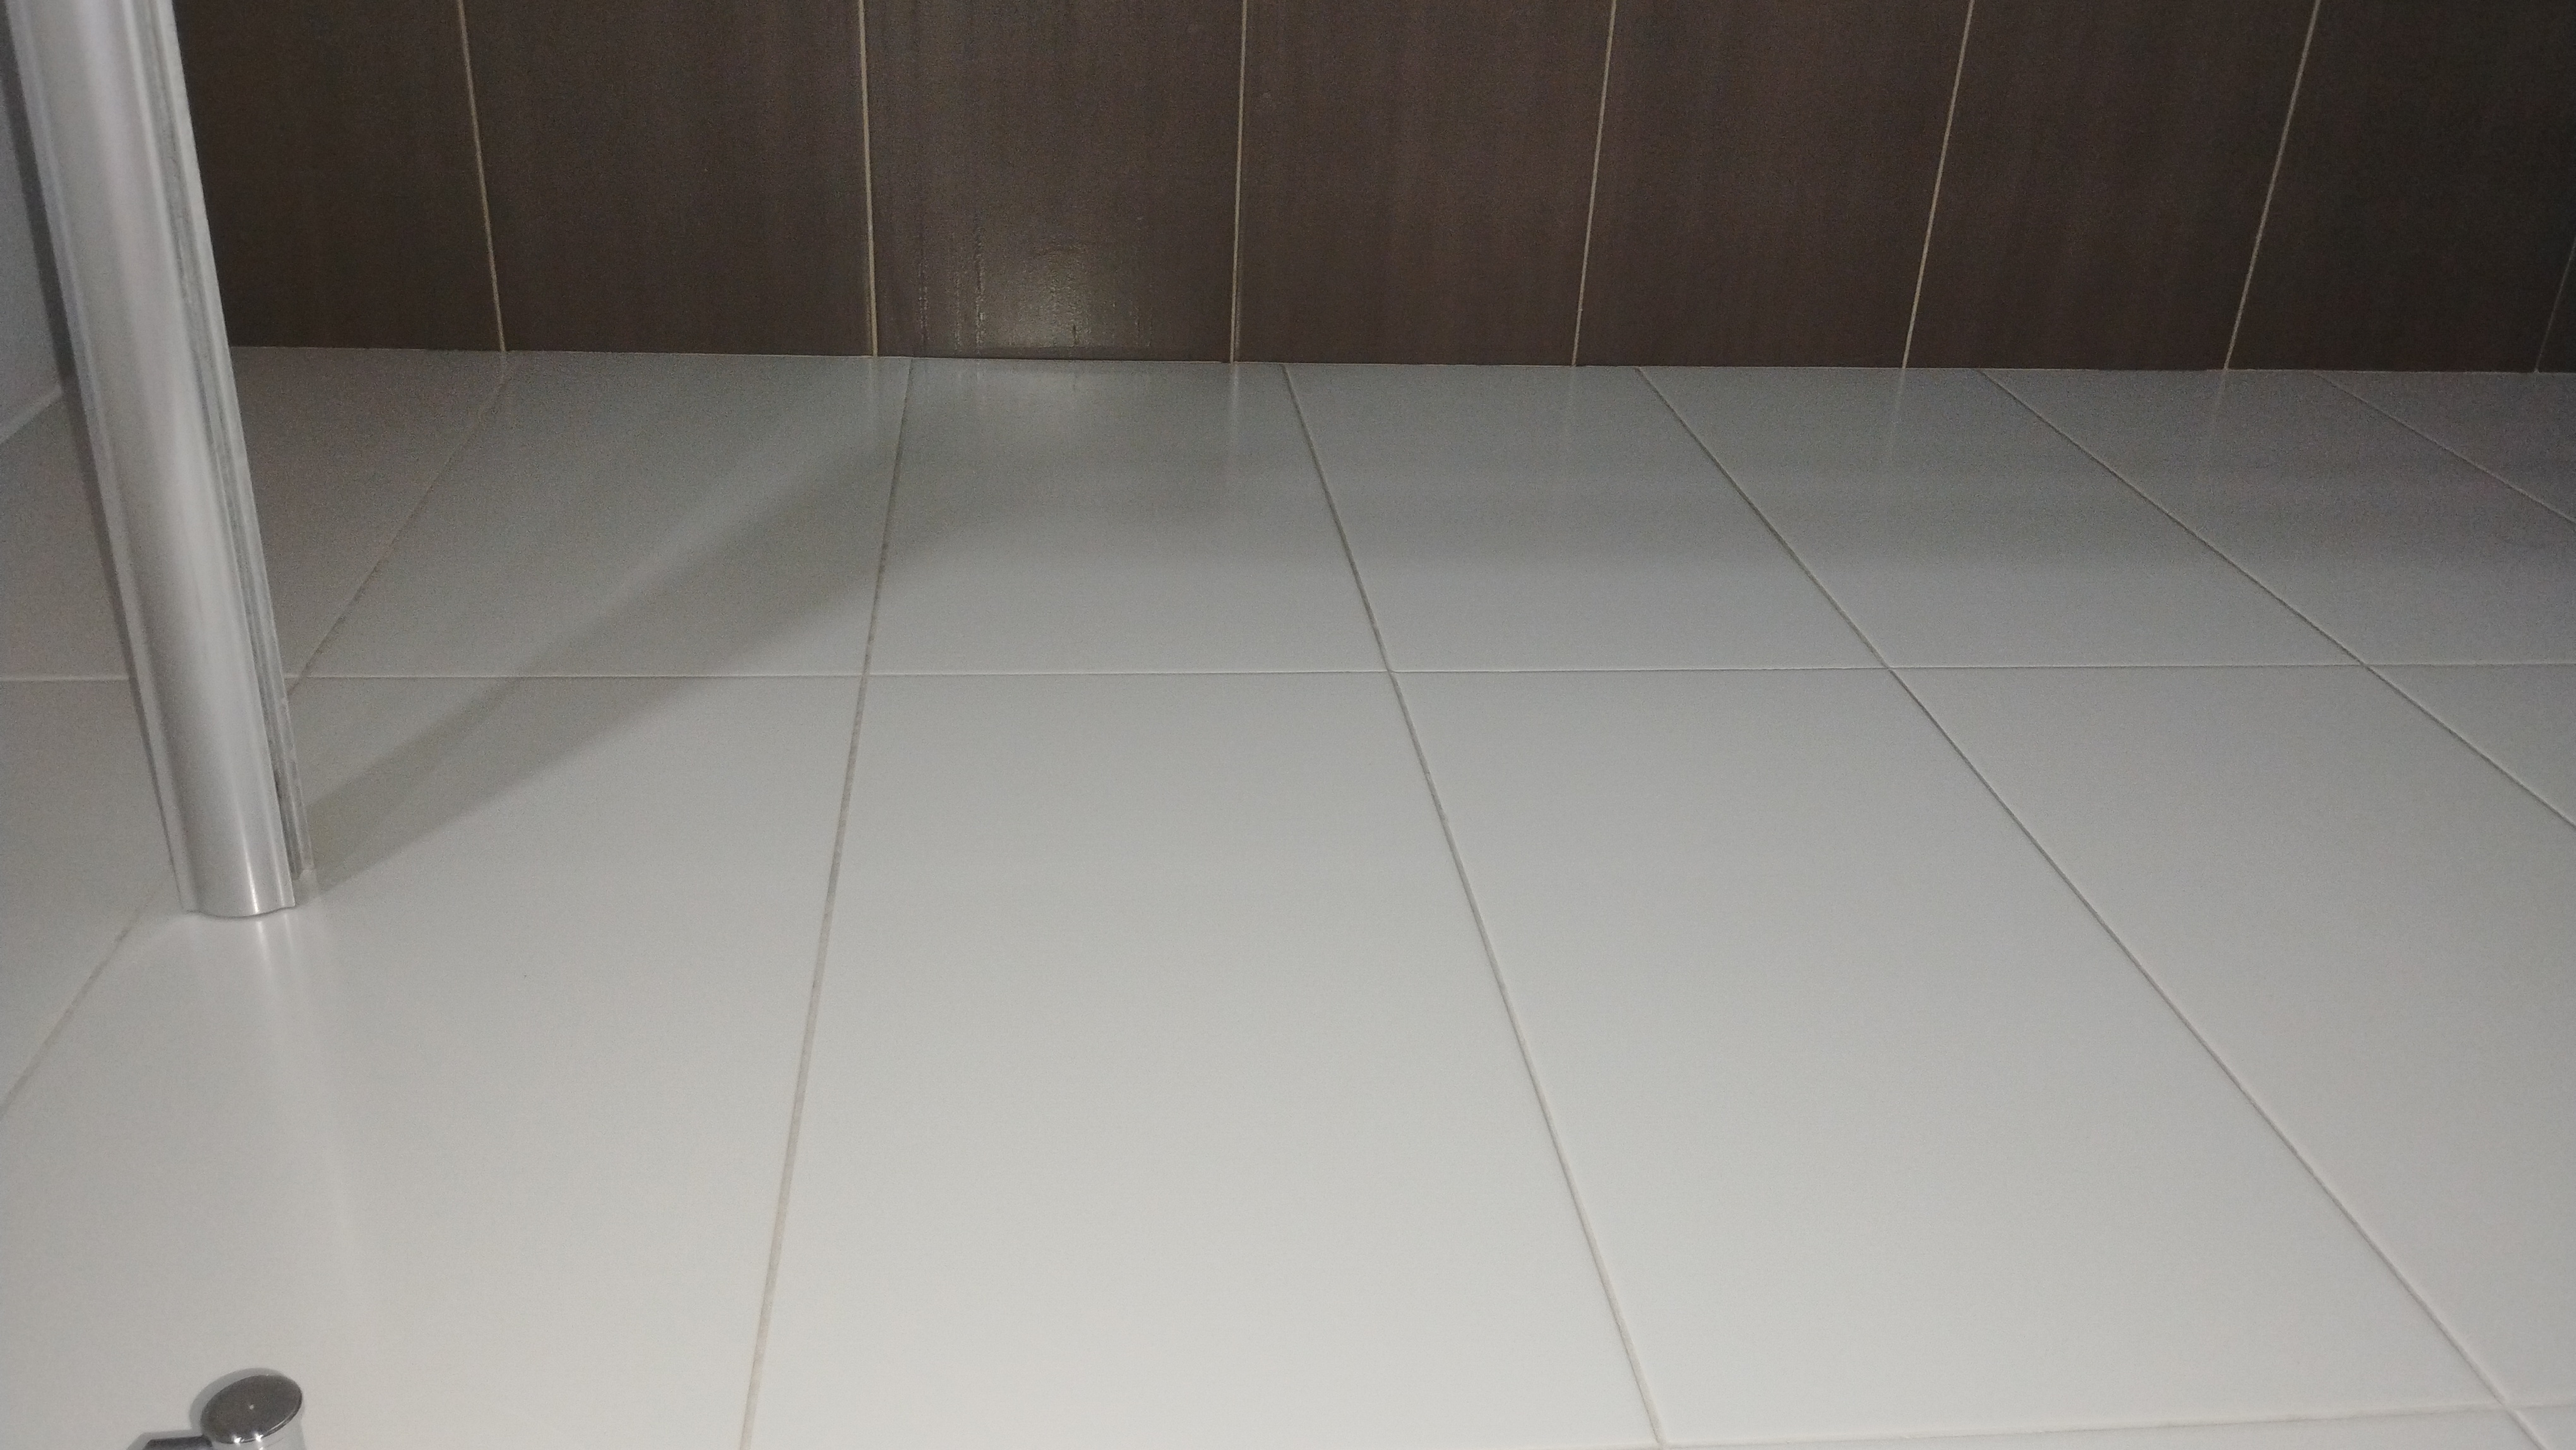
\includegraphics[width=\linewidth]{../img/IMG_20251109_151518214.jpg}\\[2pt]{\footnotesize\color{primary!60!black}Foto~24 -- 15:15:18}} \\[4pt]
\end{tabular}
\caption{Lavamanos — Grifería, Mesón y Sellos Perimetrales: Fotos 19 al 24.}\end{figure}
\newpage
\begin{figure}[H]
\centering
\begin{tabular}{cc}
\parbox{0.45\textwidth}{\centering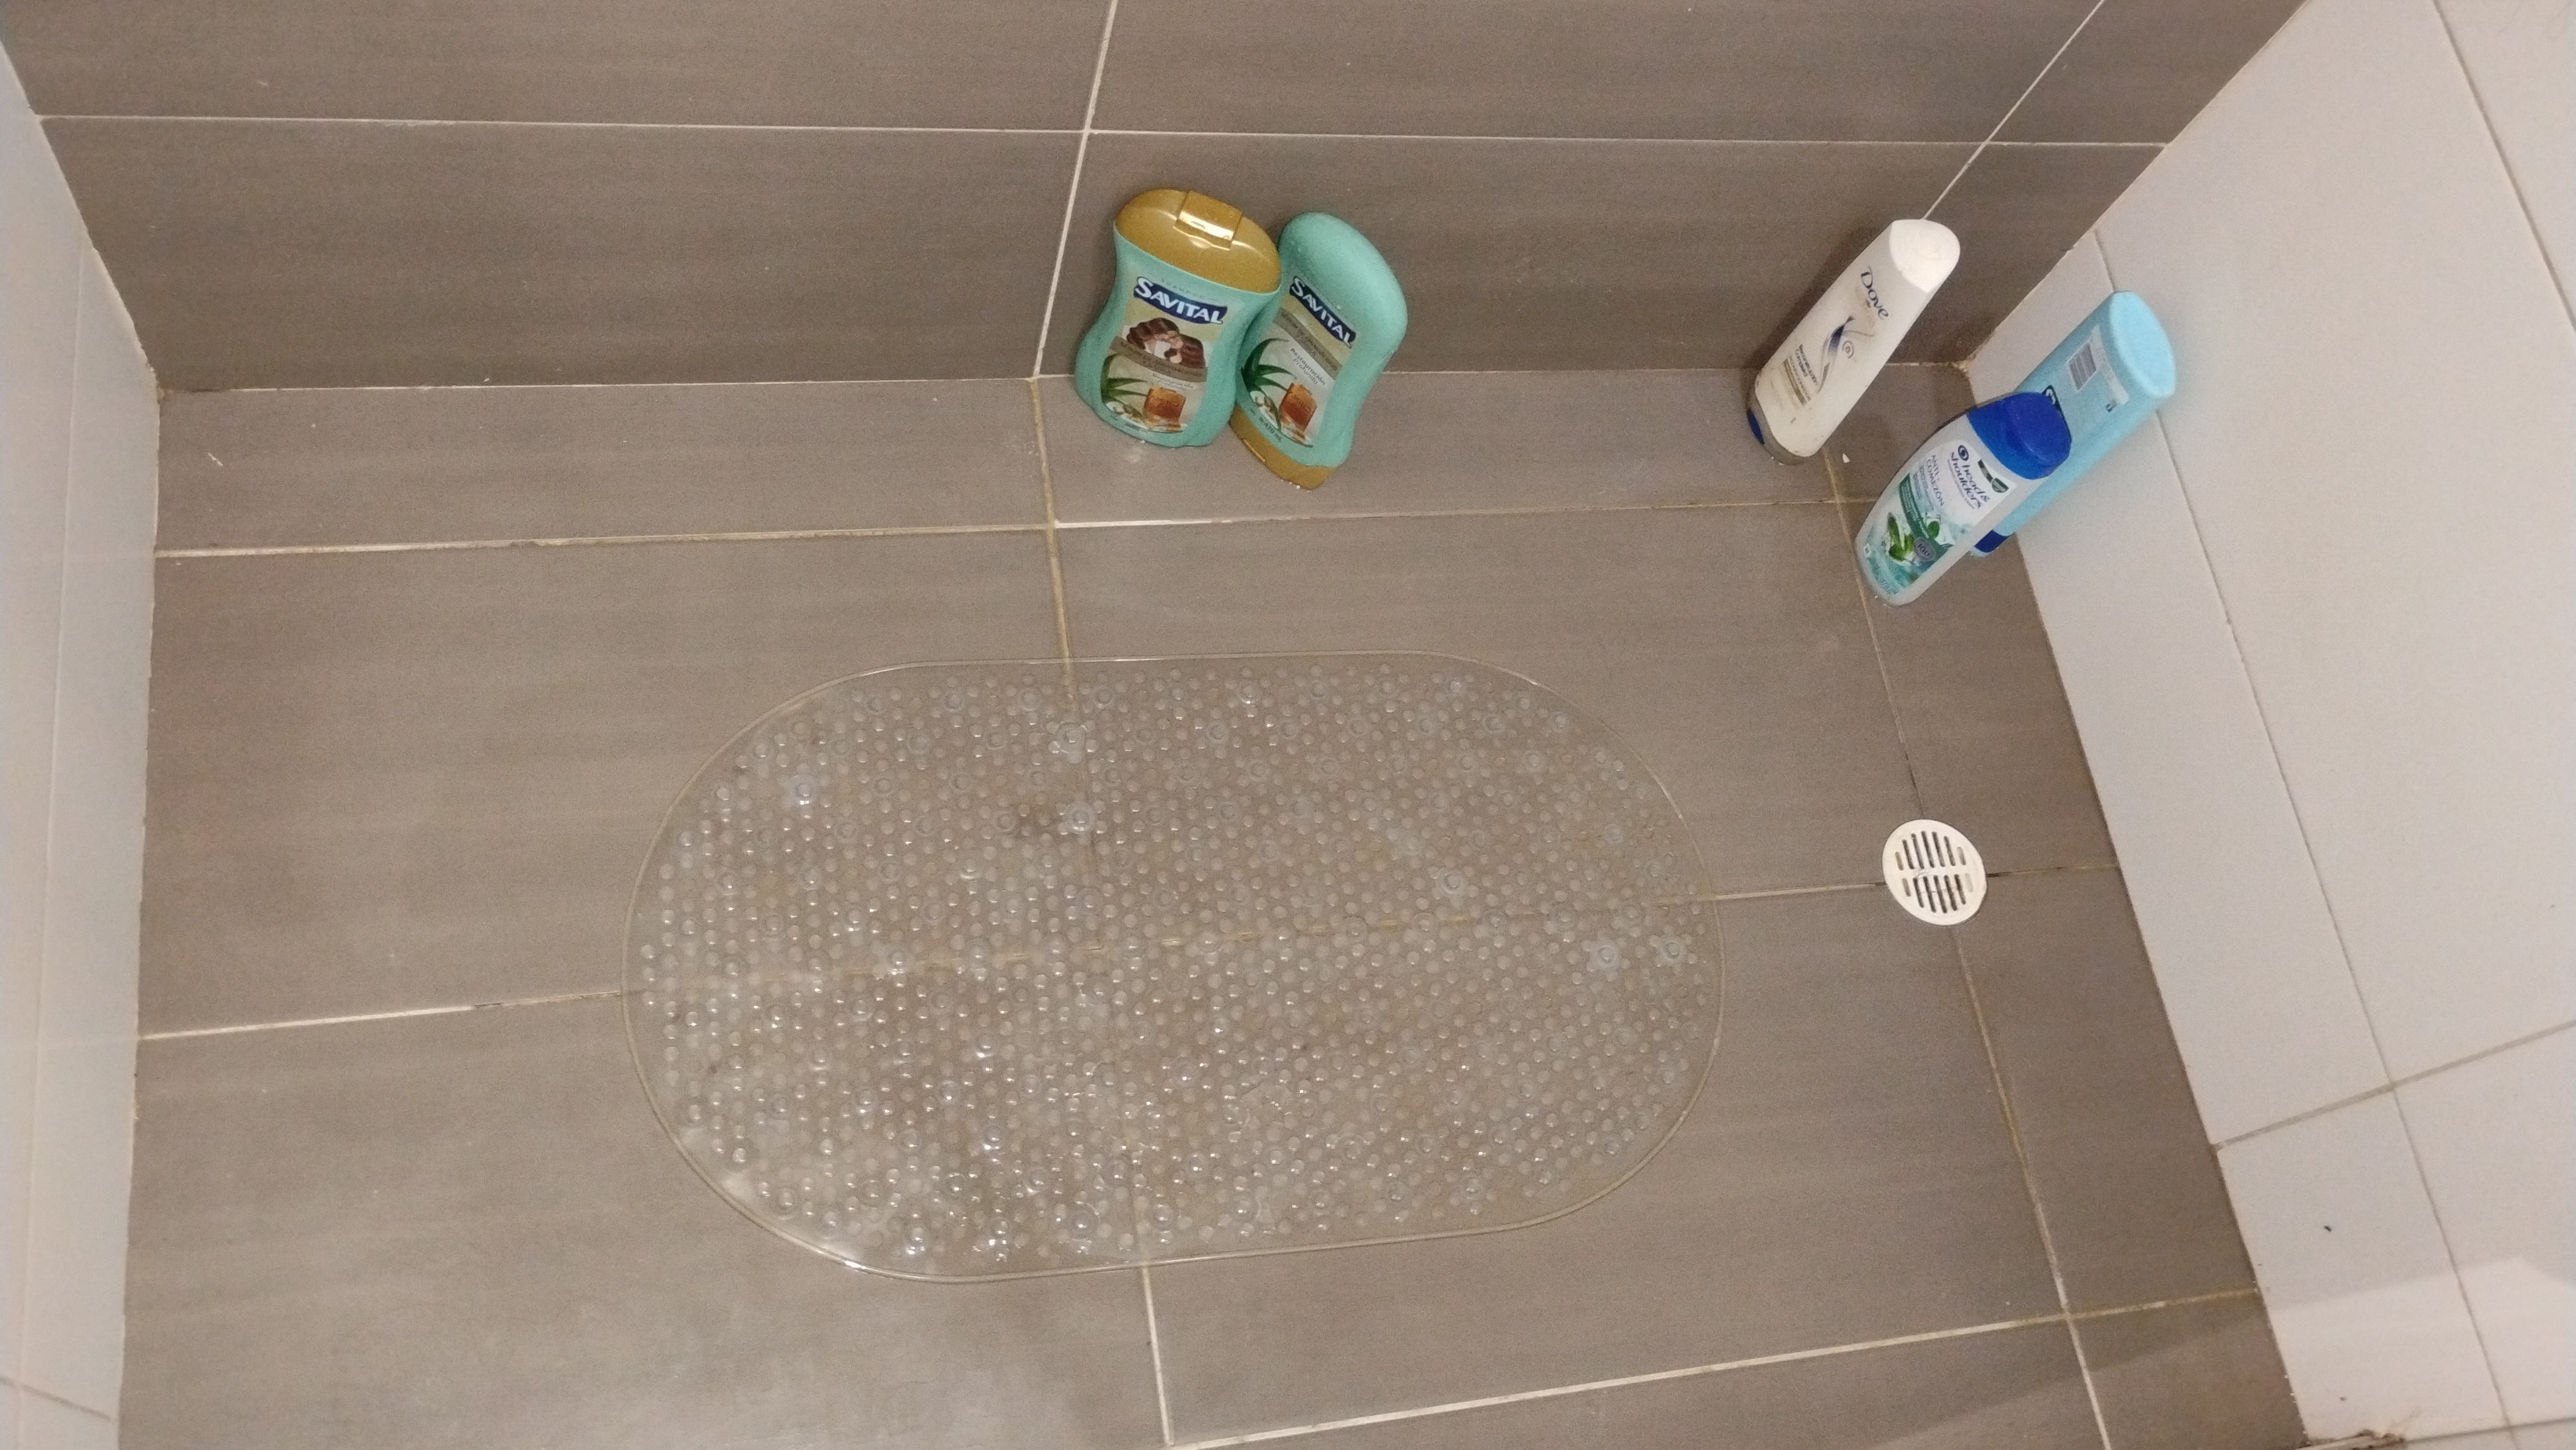
\includegraphics[width=\linewidth]{../img/IMG_20251109_151526704.jpg}\\[2pt]{\footnotesize\color{primary!60!black}Foto~25 -- 15:15:26}} & \parbox{0.45\textwidth}{\centering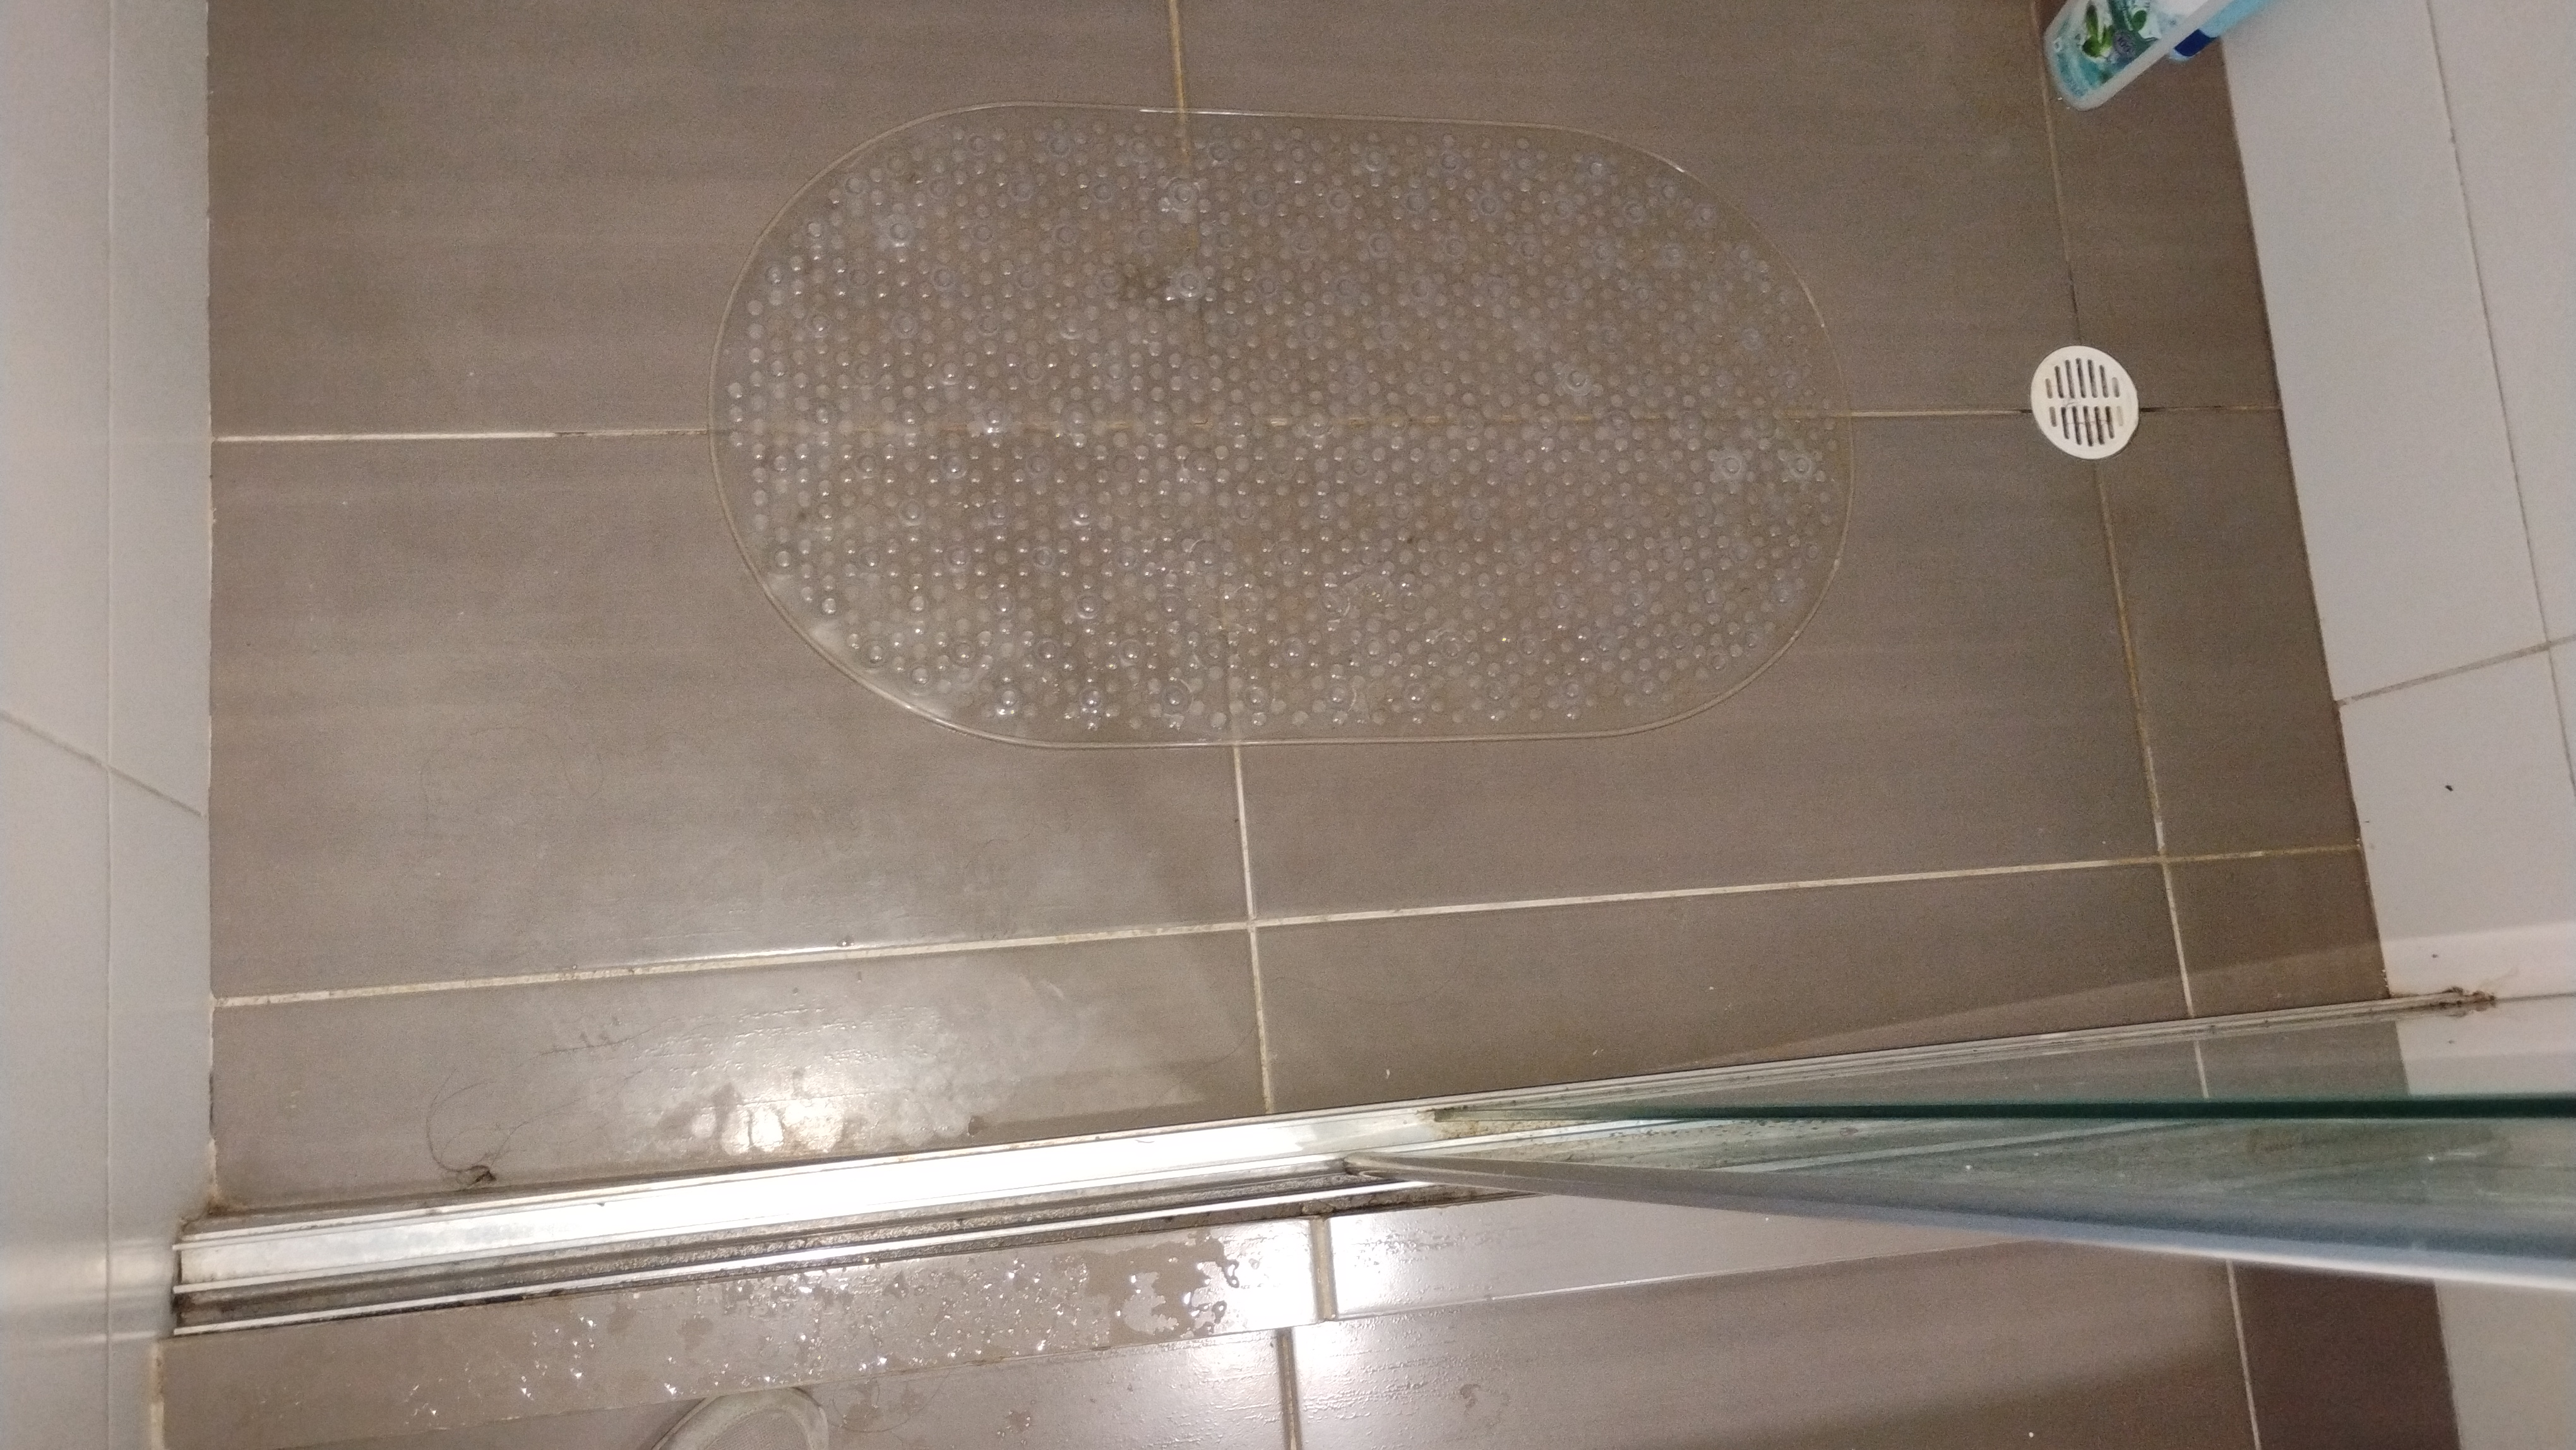
\includegraphics[width=\linewidth]{../img/IMG_20251109_151530083.jpg}\\[2pt]{\footnotesize\color{primary!60!black}Foto~26 -- 15:15:30}} \\[4pt]
\parbox{0.45\textwidth}{\centering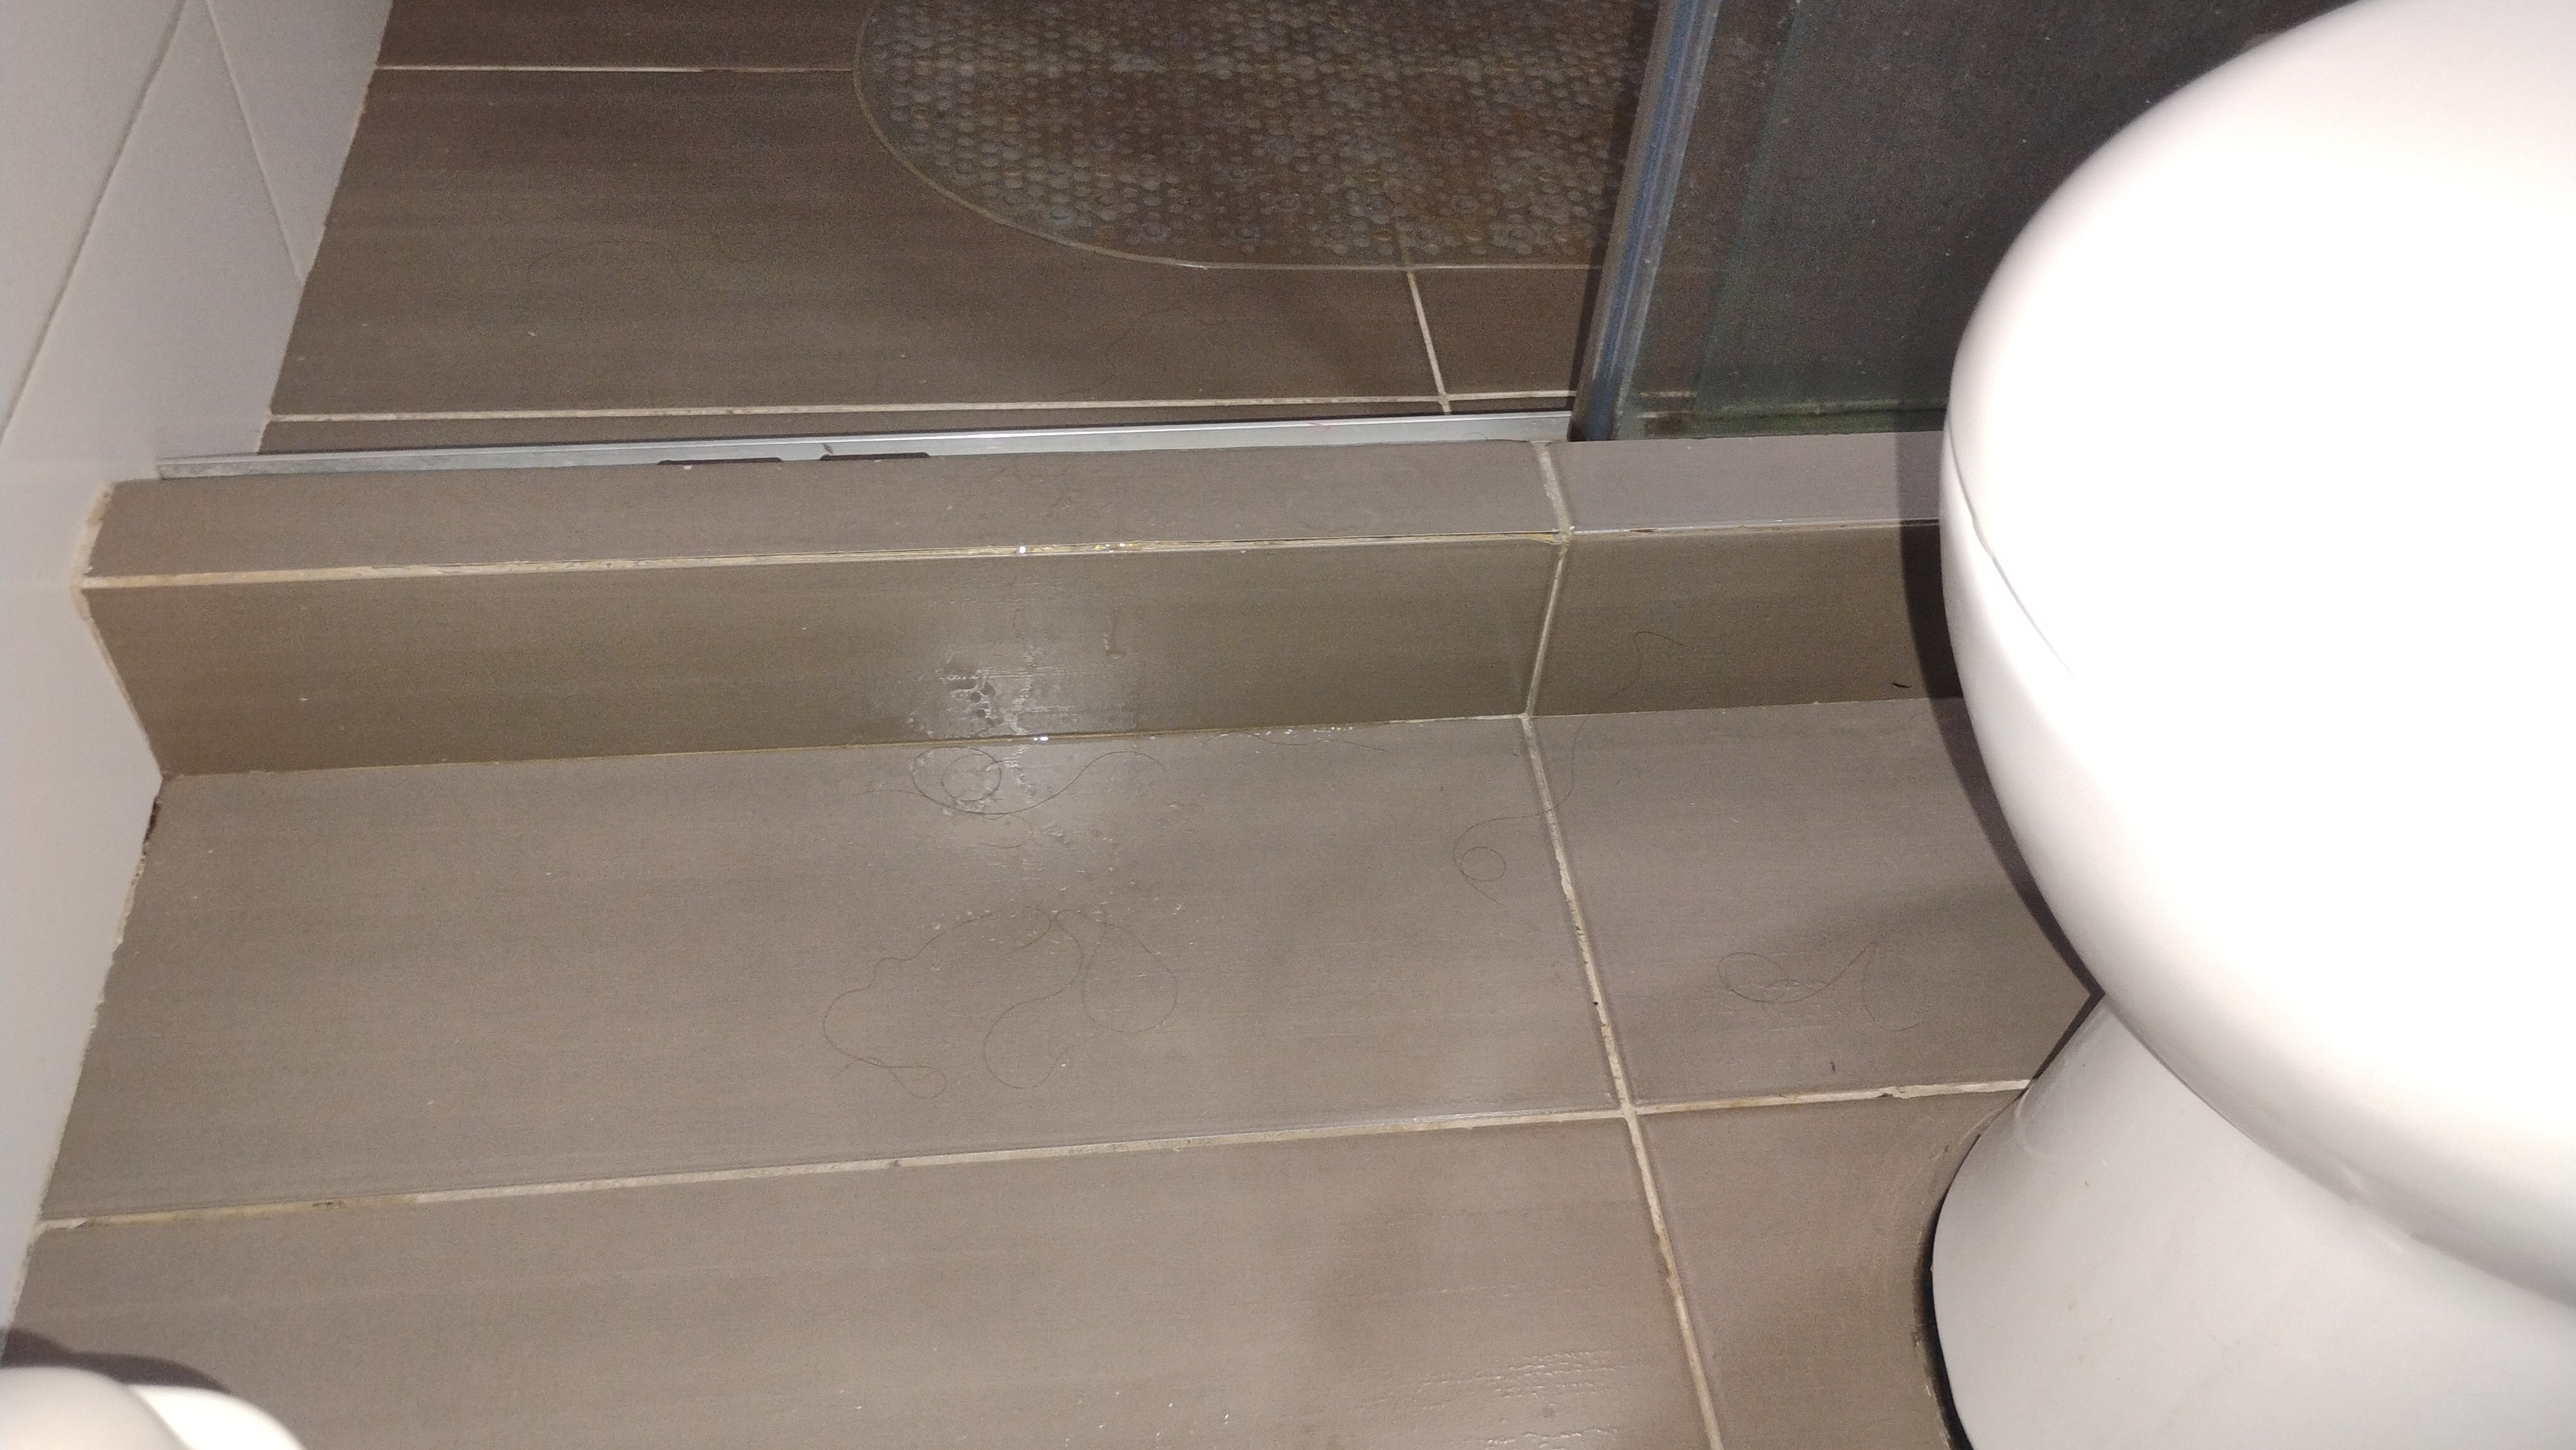
\includegraphics[width=\linewidth]{../img/IMG_20251109_151559560.jpg}\\[2pt]{\footnotesize\color{primary!60!black}Foto~27 -- 15:15:59}} & \parbox{0.45\textwidth}{\centering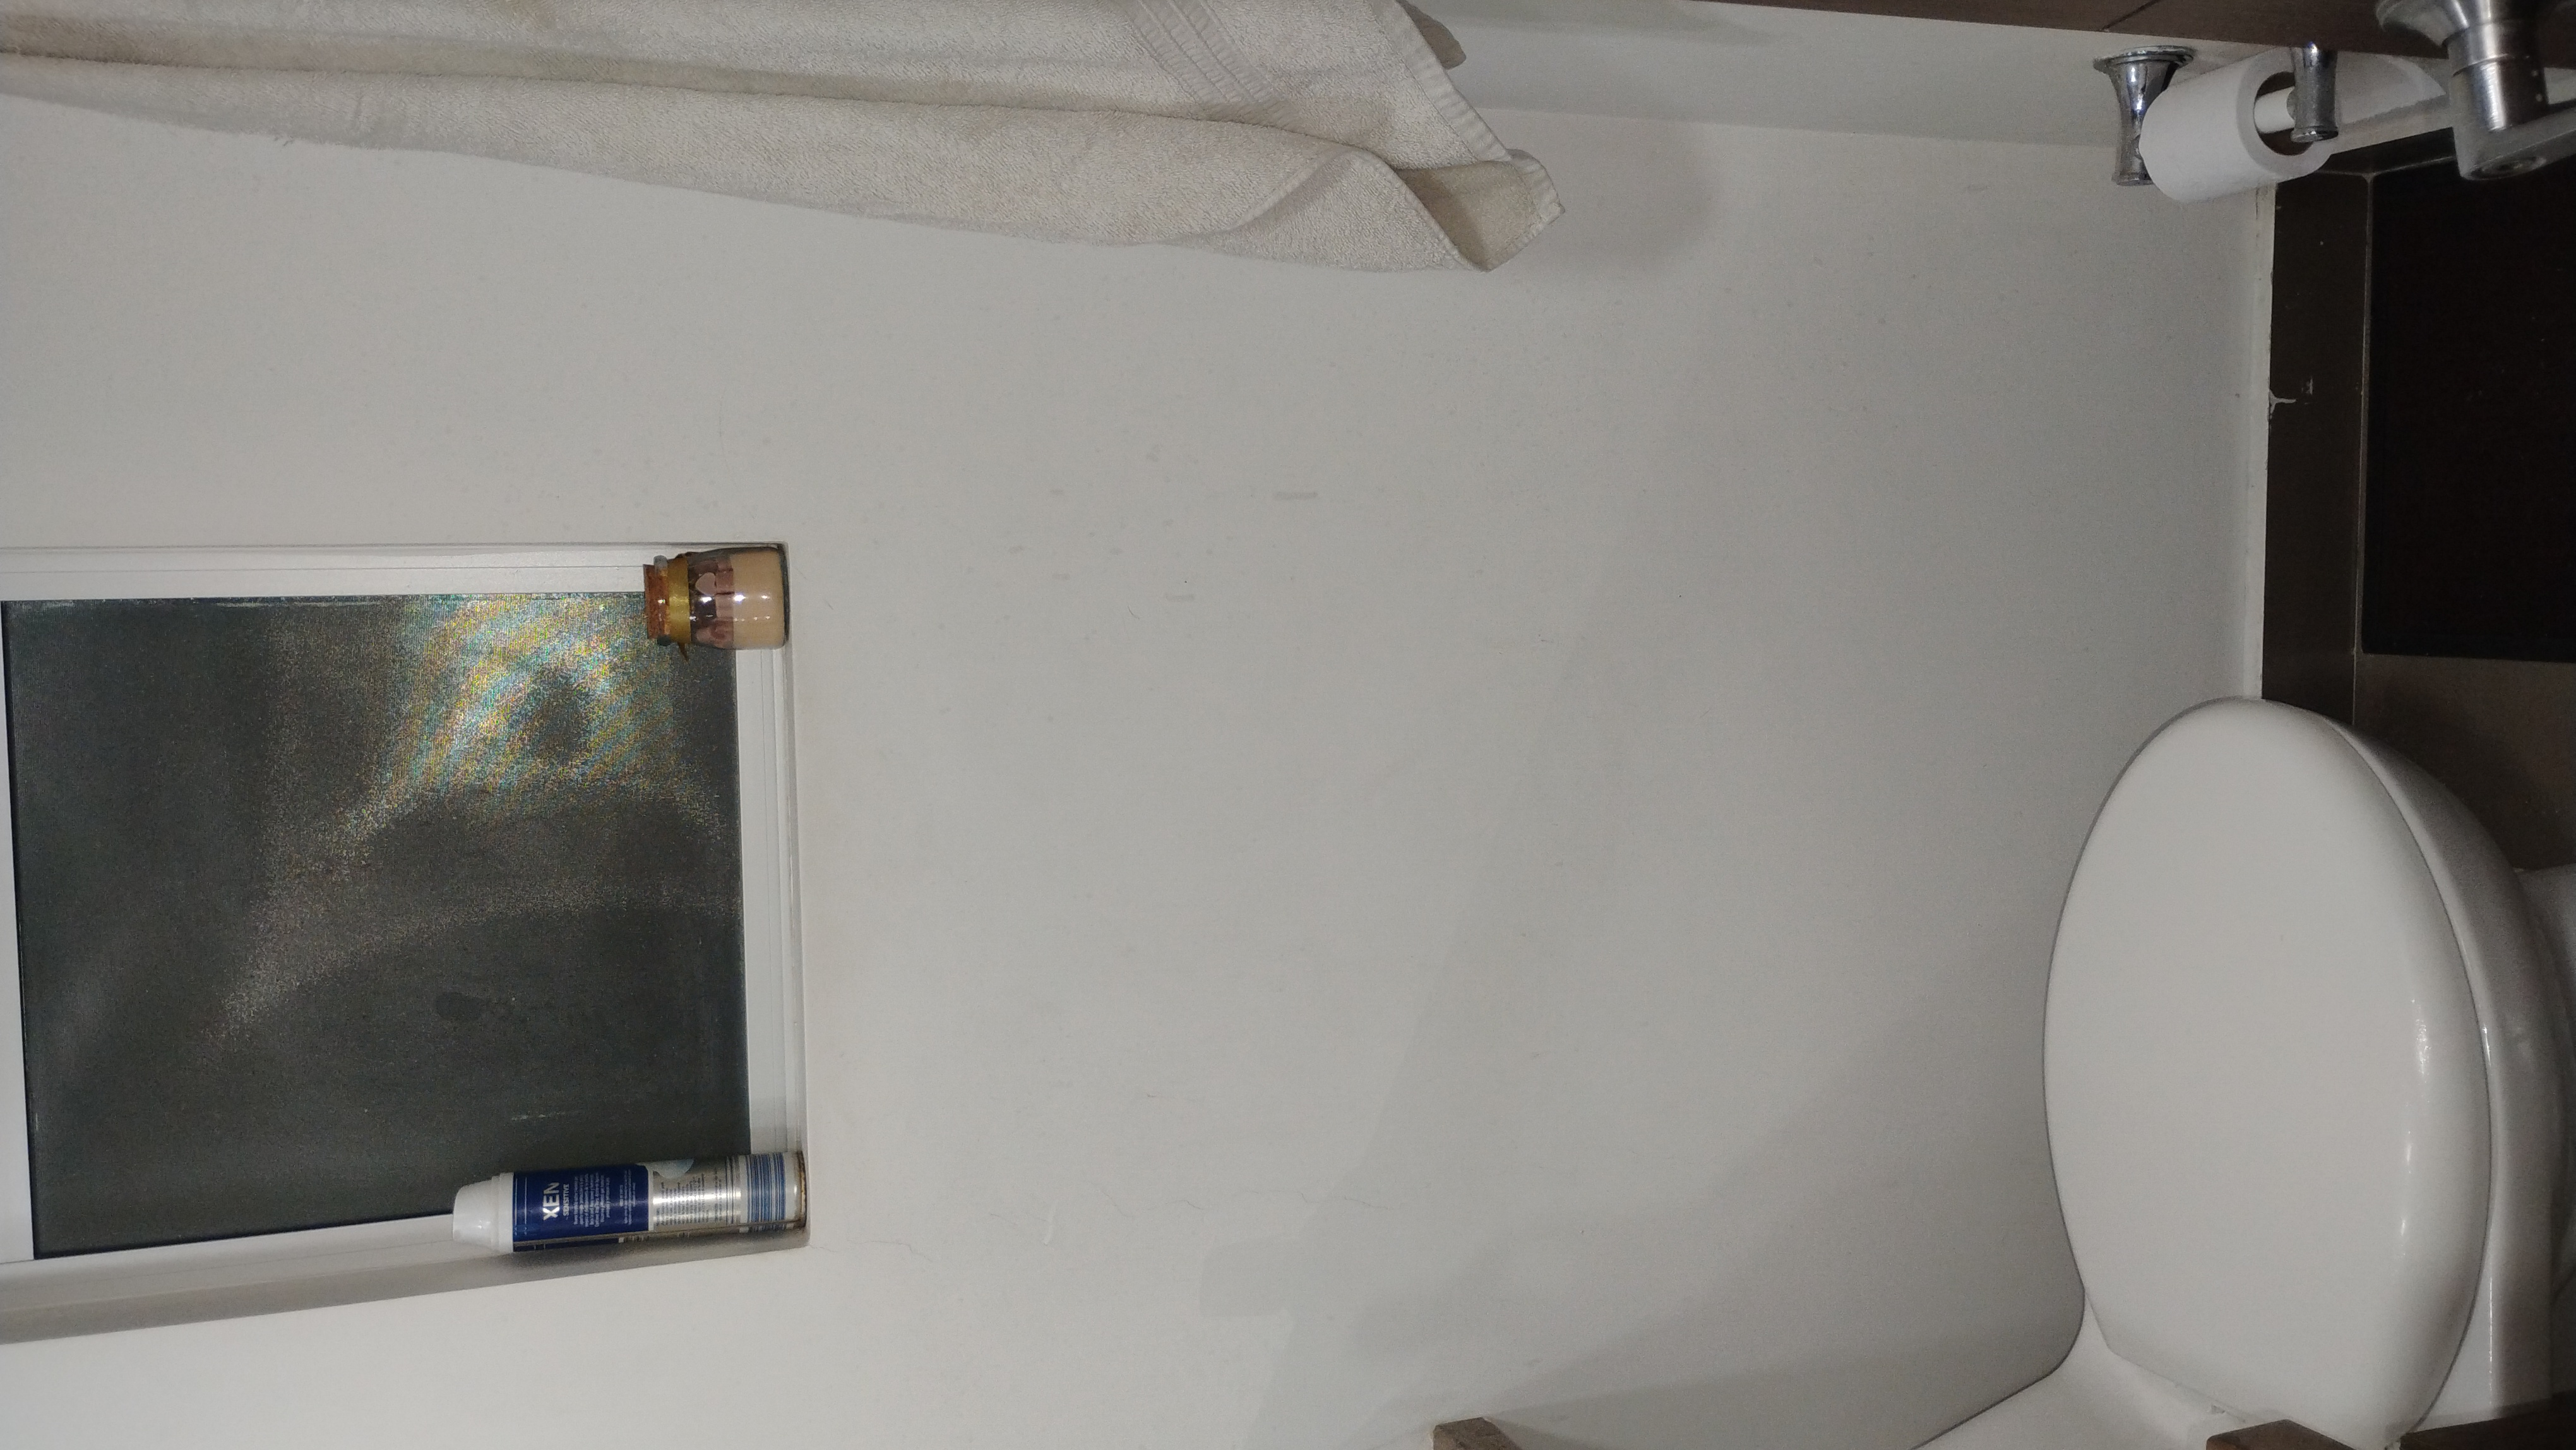
\includegraphics[width=\linewidth]{../img/IMG_20251109_151729556.jpg}\\[2pt]{\footnotesize\color{primary!60!black}Foto~28 -- 15:17:29}} \\[4pt]
\parbox{0.45\textwidth}{\centering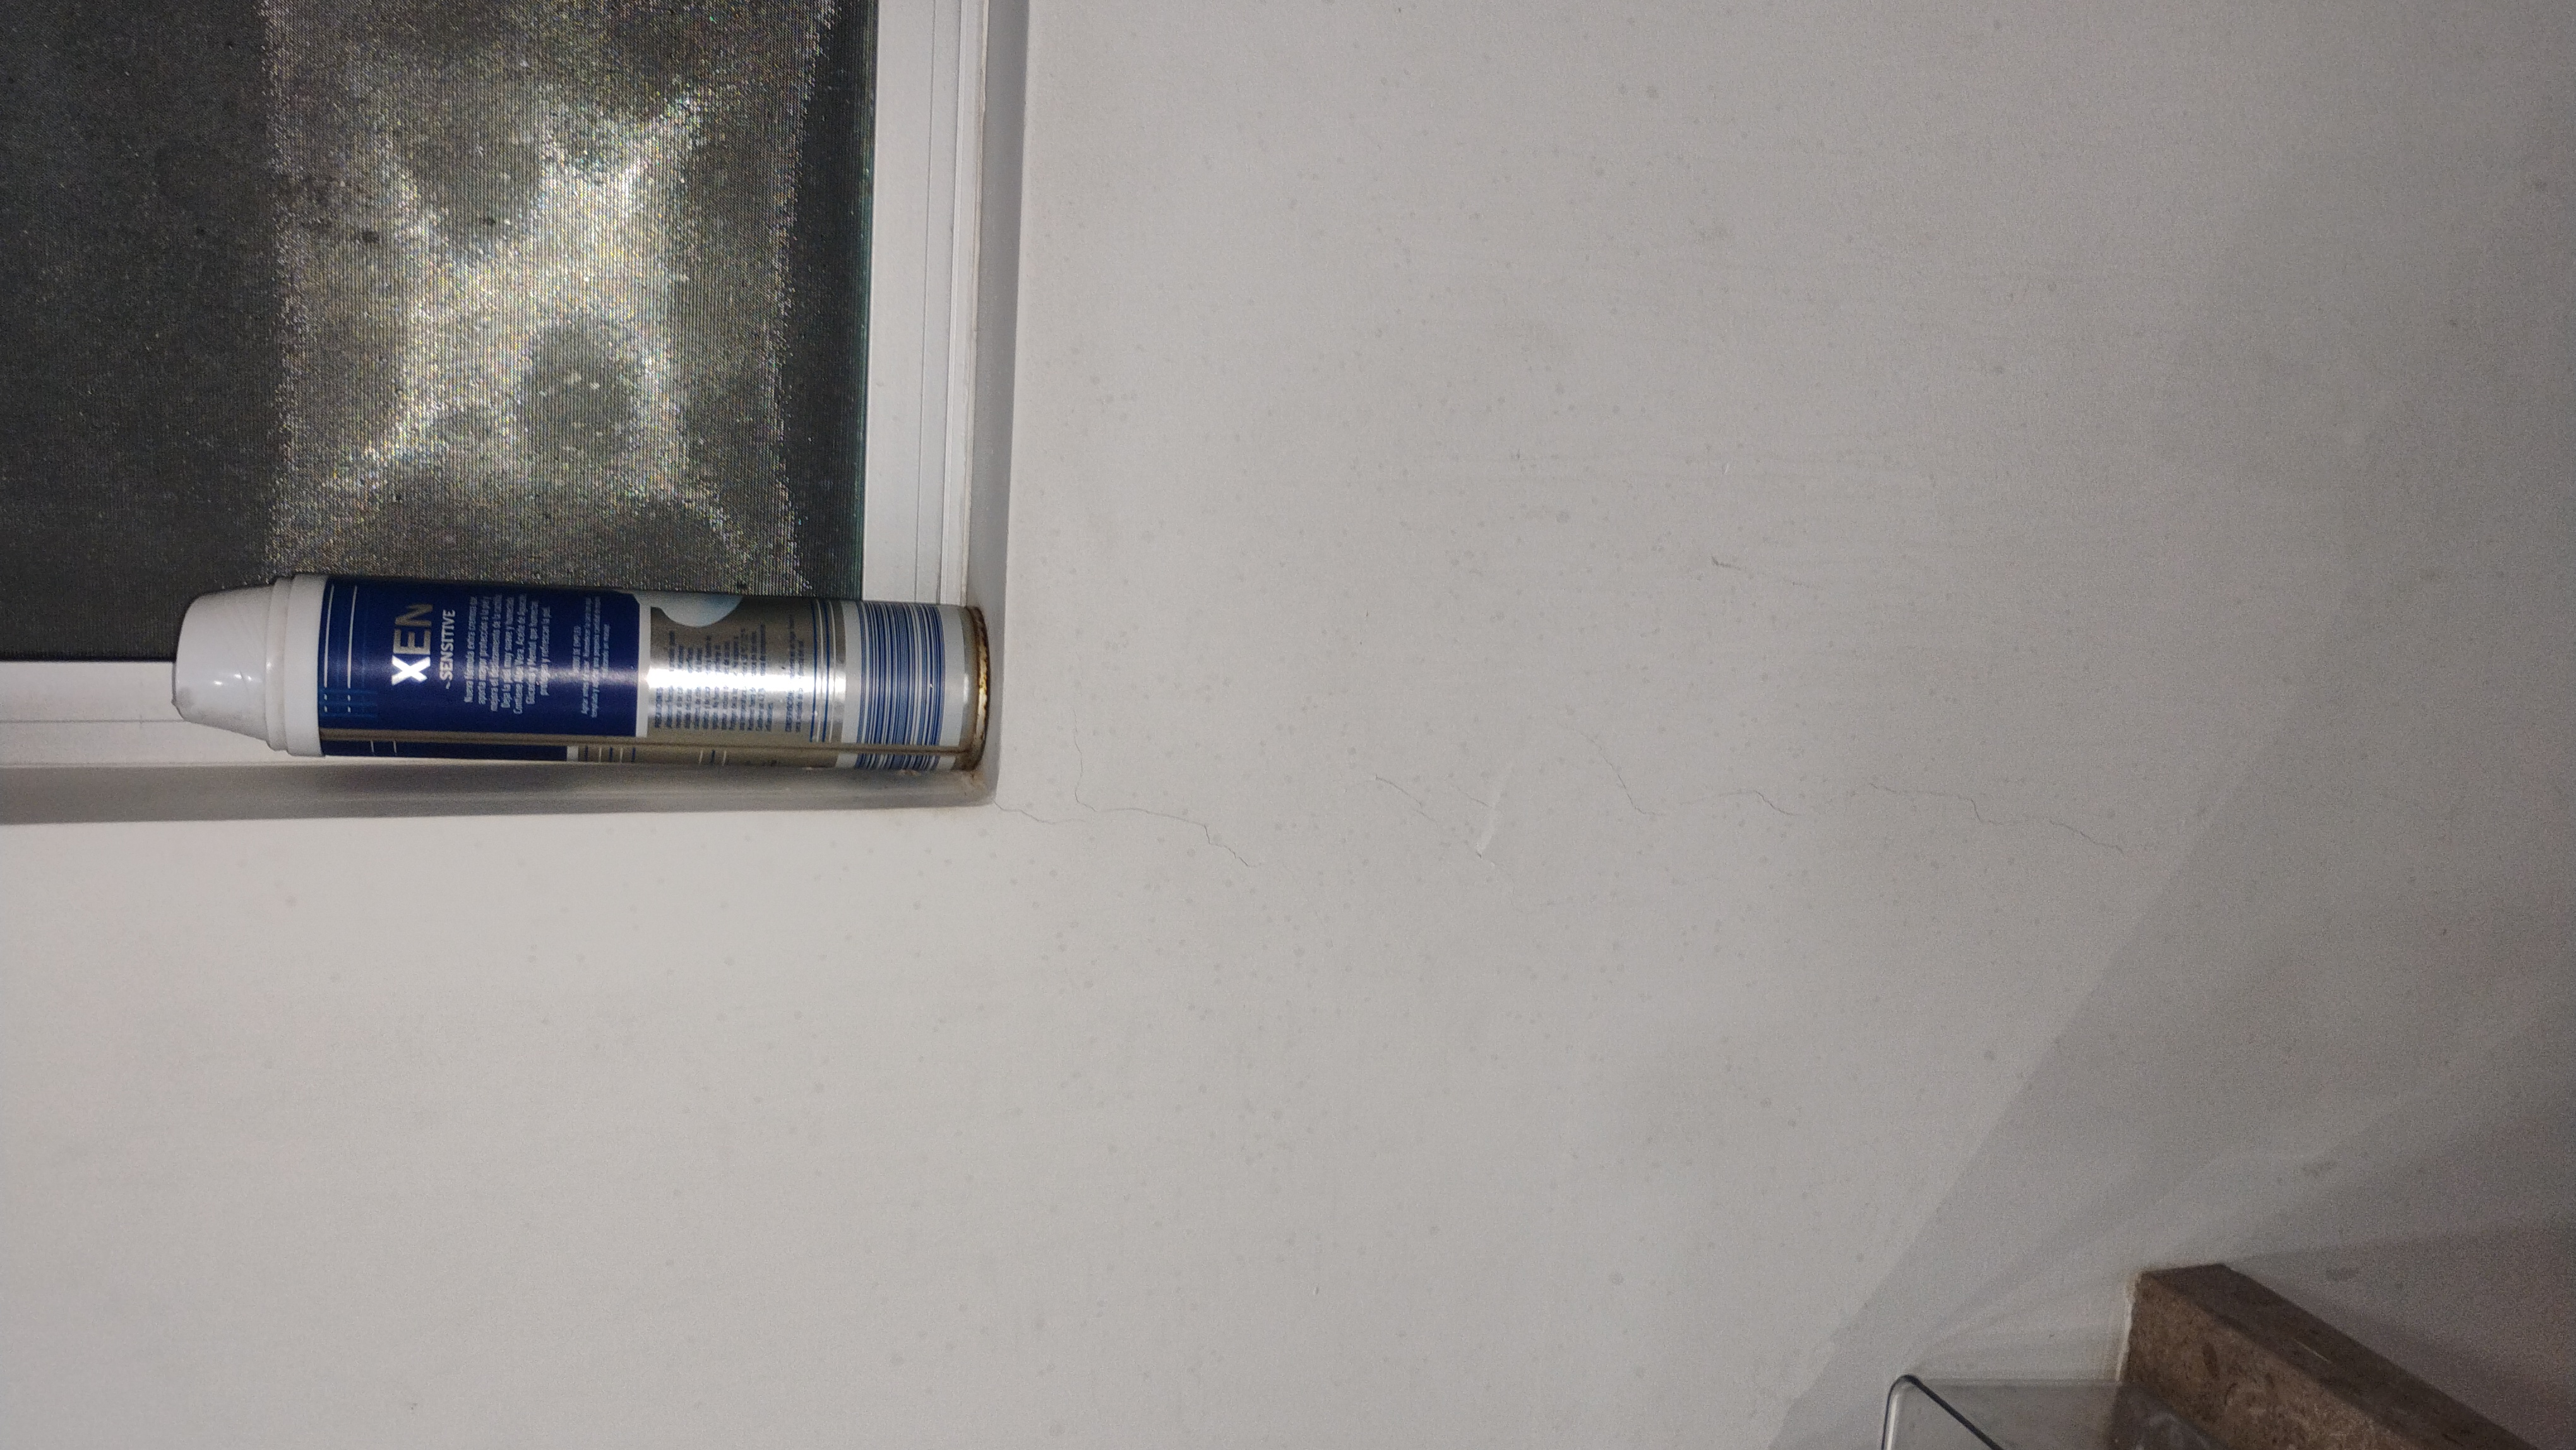
\includegraphics[width=\linewidth]{../img/IMG_20251109_151733859.jpg}\\[2pt]{\footnotesize\color{primary!60!black}Foto~29 -- 15:17:33}} & \parbox{0.45\textwidth}{\centering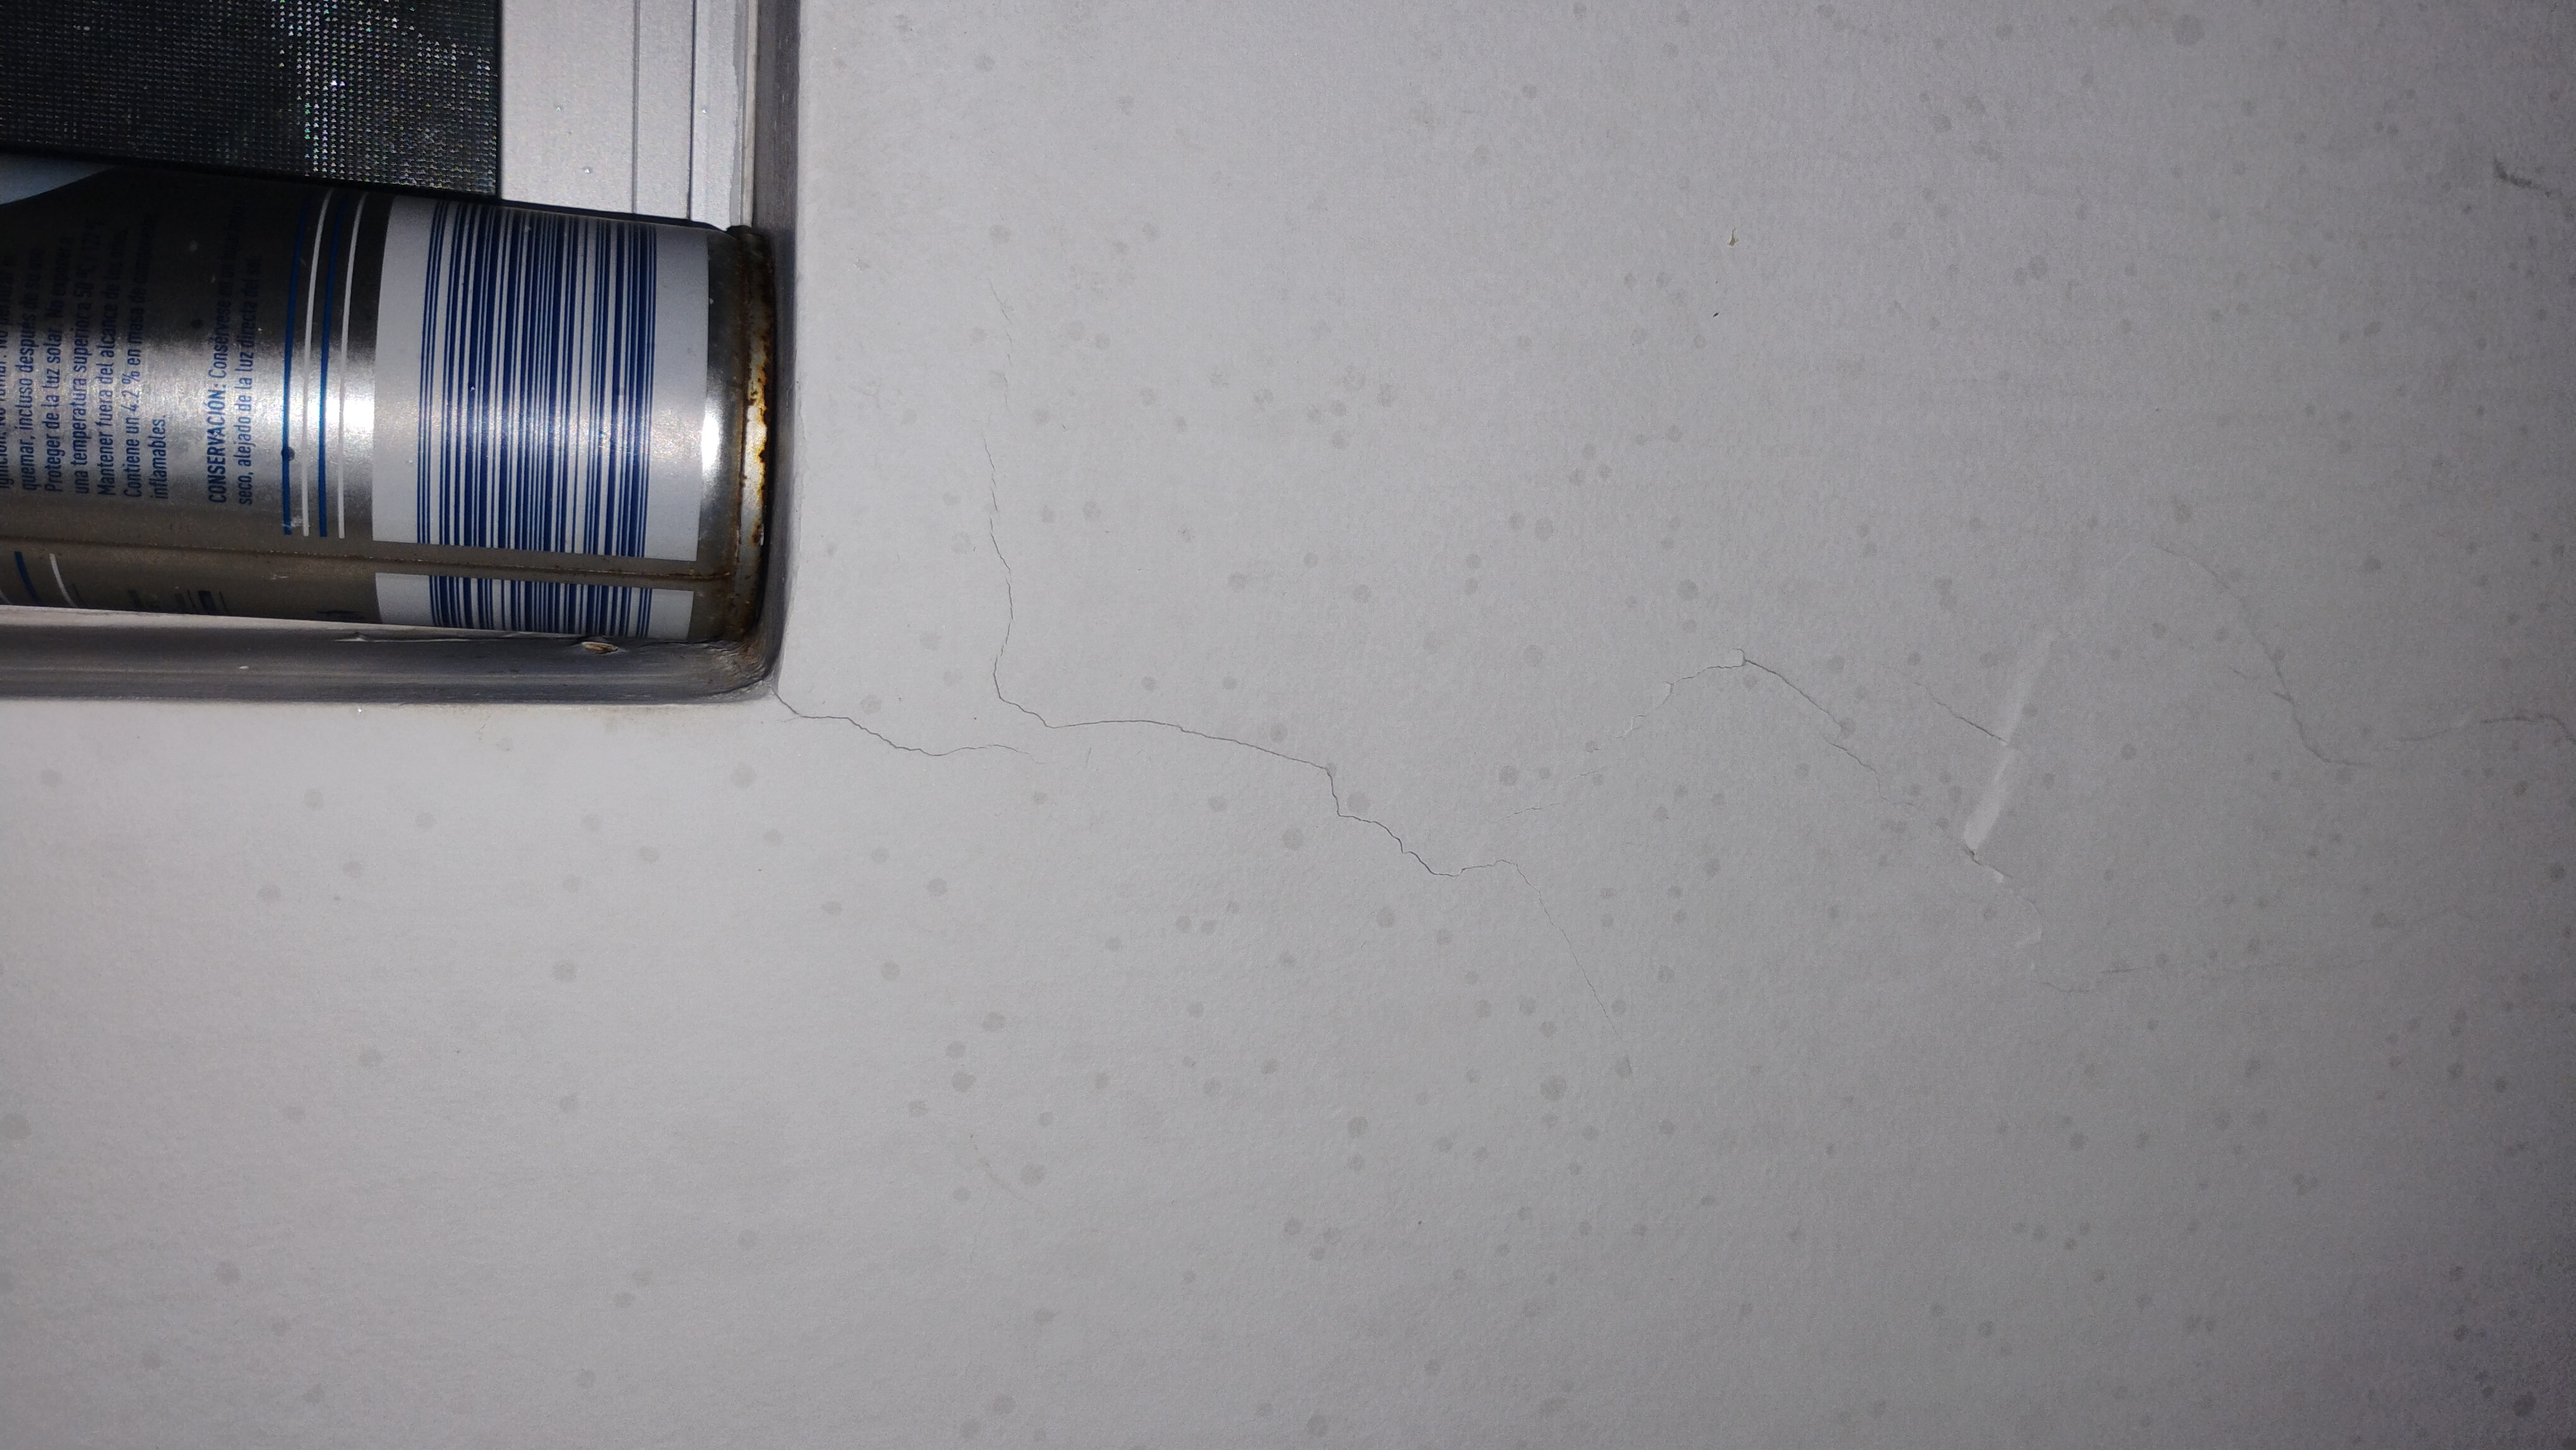
\includegraphics[width=\linewidth]{../img/IMG_20251109_151739018.jpg}\\[2pt]{\footnotesize\color{primary!60!black}Foto~30 -- 15:17:39}} \\[4pt]
\end{tabular}
\caption{Sanitario — Base, Junta Piso-Pared y Empaques: Fotos 25 al 30.}\end{figure}
\newpage
\section{Baño 2}
\noindent\textbf{Estado general:} REGULAR A MALO.
\medskip
\noindent\textbf{Patologías identificadas:}
\begin{itemize}[leftmargin=*,nosep]
  \item \textbf{Humedad por filtración} en la zona de la ducha — el paño occidental presenta desprendimiento de enchape en un área aproximada de 30 $\times$ 50 cm, con pérdida total de adherencia al mortero de pega y sonido a hueco característico.
  \item \textbf{Eflorescencia masiva} en la totalidad del paño de la ducha — cristalización de sales en las juntas y sobre la superficie del porcelanato, indicativa de filtración continua desde la instalación hidrosanitaria.
  \item \textbf{Fisura diagonal} de 22 cm en el muro oriental, coincidente con el punto de anclaje del soporte de la ducha — posible concentración de esfuerzos por vibración o fatiga.
  \item \textbf{Corrosión severa} en la válvula mezcladora y ducha teléfono — pérdida de cromado superficial con puntos de oxidación profunda que comprometen la estanqueidad del conjunto.
  \item \textbf{Desprendimiento de pañete} en el cielorraso, con manchas de humedad intermitente asociadas a posibles filtraciones desde el nivel superior.
  \item \textbf{Sellos sanitarios inexistentes} en la base del inodoro — se evidencia acumulación de suciedad, orina cristalizada y colonia de hongos en la interfaz porcelana-piso.
  \item \textbf{Deterioro de la lechada} en el 60\% del área de piso, con pérdida de material y huecos de hasta 3 mm de profundidad, generando cavidades que acumulan agua y suciedad.
\end{itemize}
\medskip
\noindent\textbf{Zonas críticas:} Ducha completa (filtración activa, desprendimiento de enchape, corrosión), base del sanitario (sellos ausentes), cielorraso (humedad intermitente), piso (lechada deteriorada).
\bigskip
\begin{figure}[H]
\centering
\begin{tabular}{cc}
\parbox{0.45\textwidth}{\centering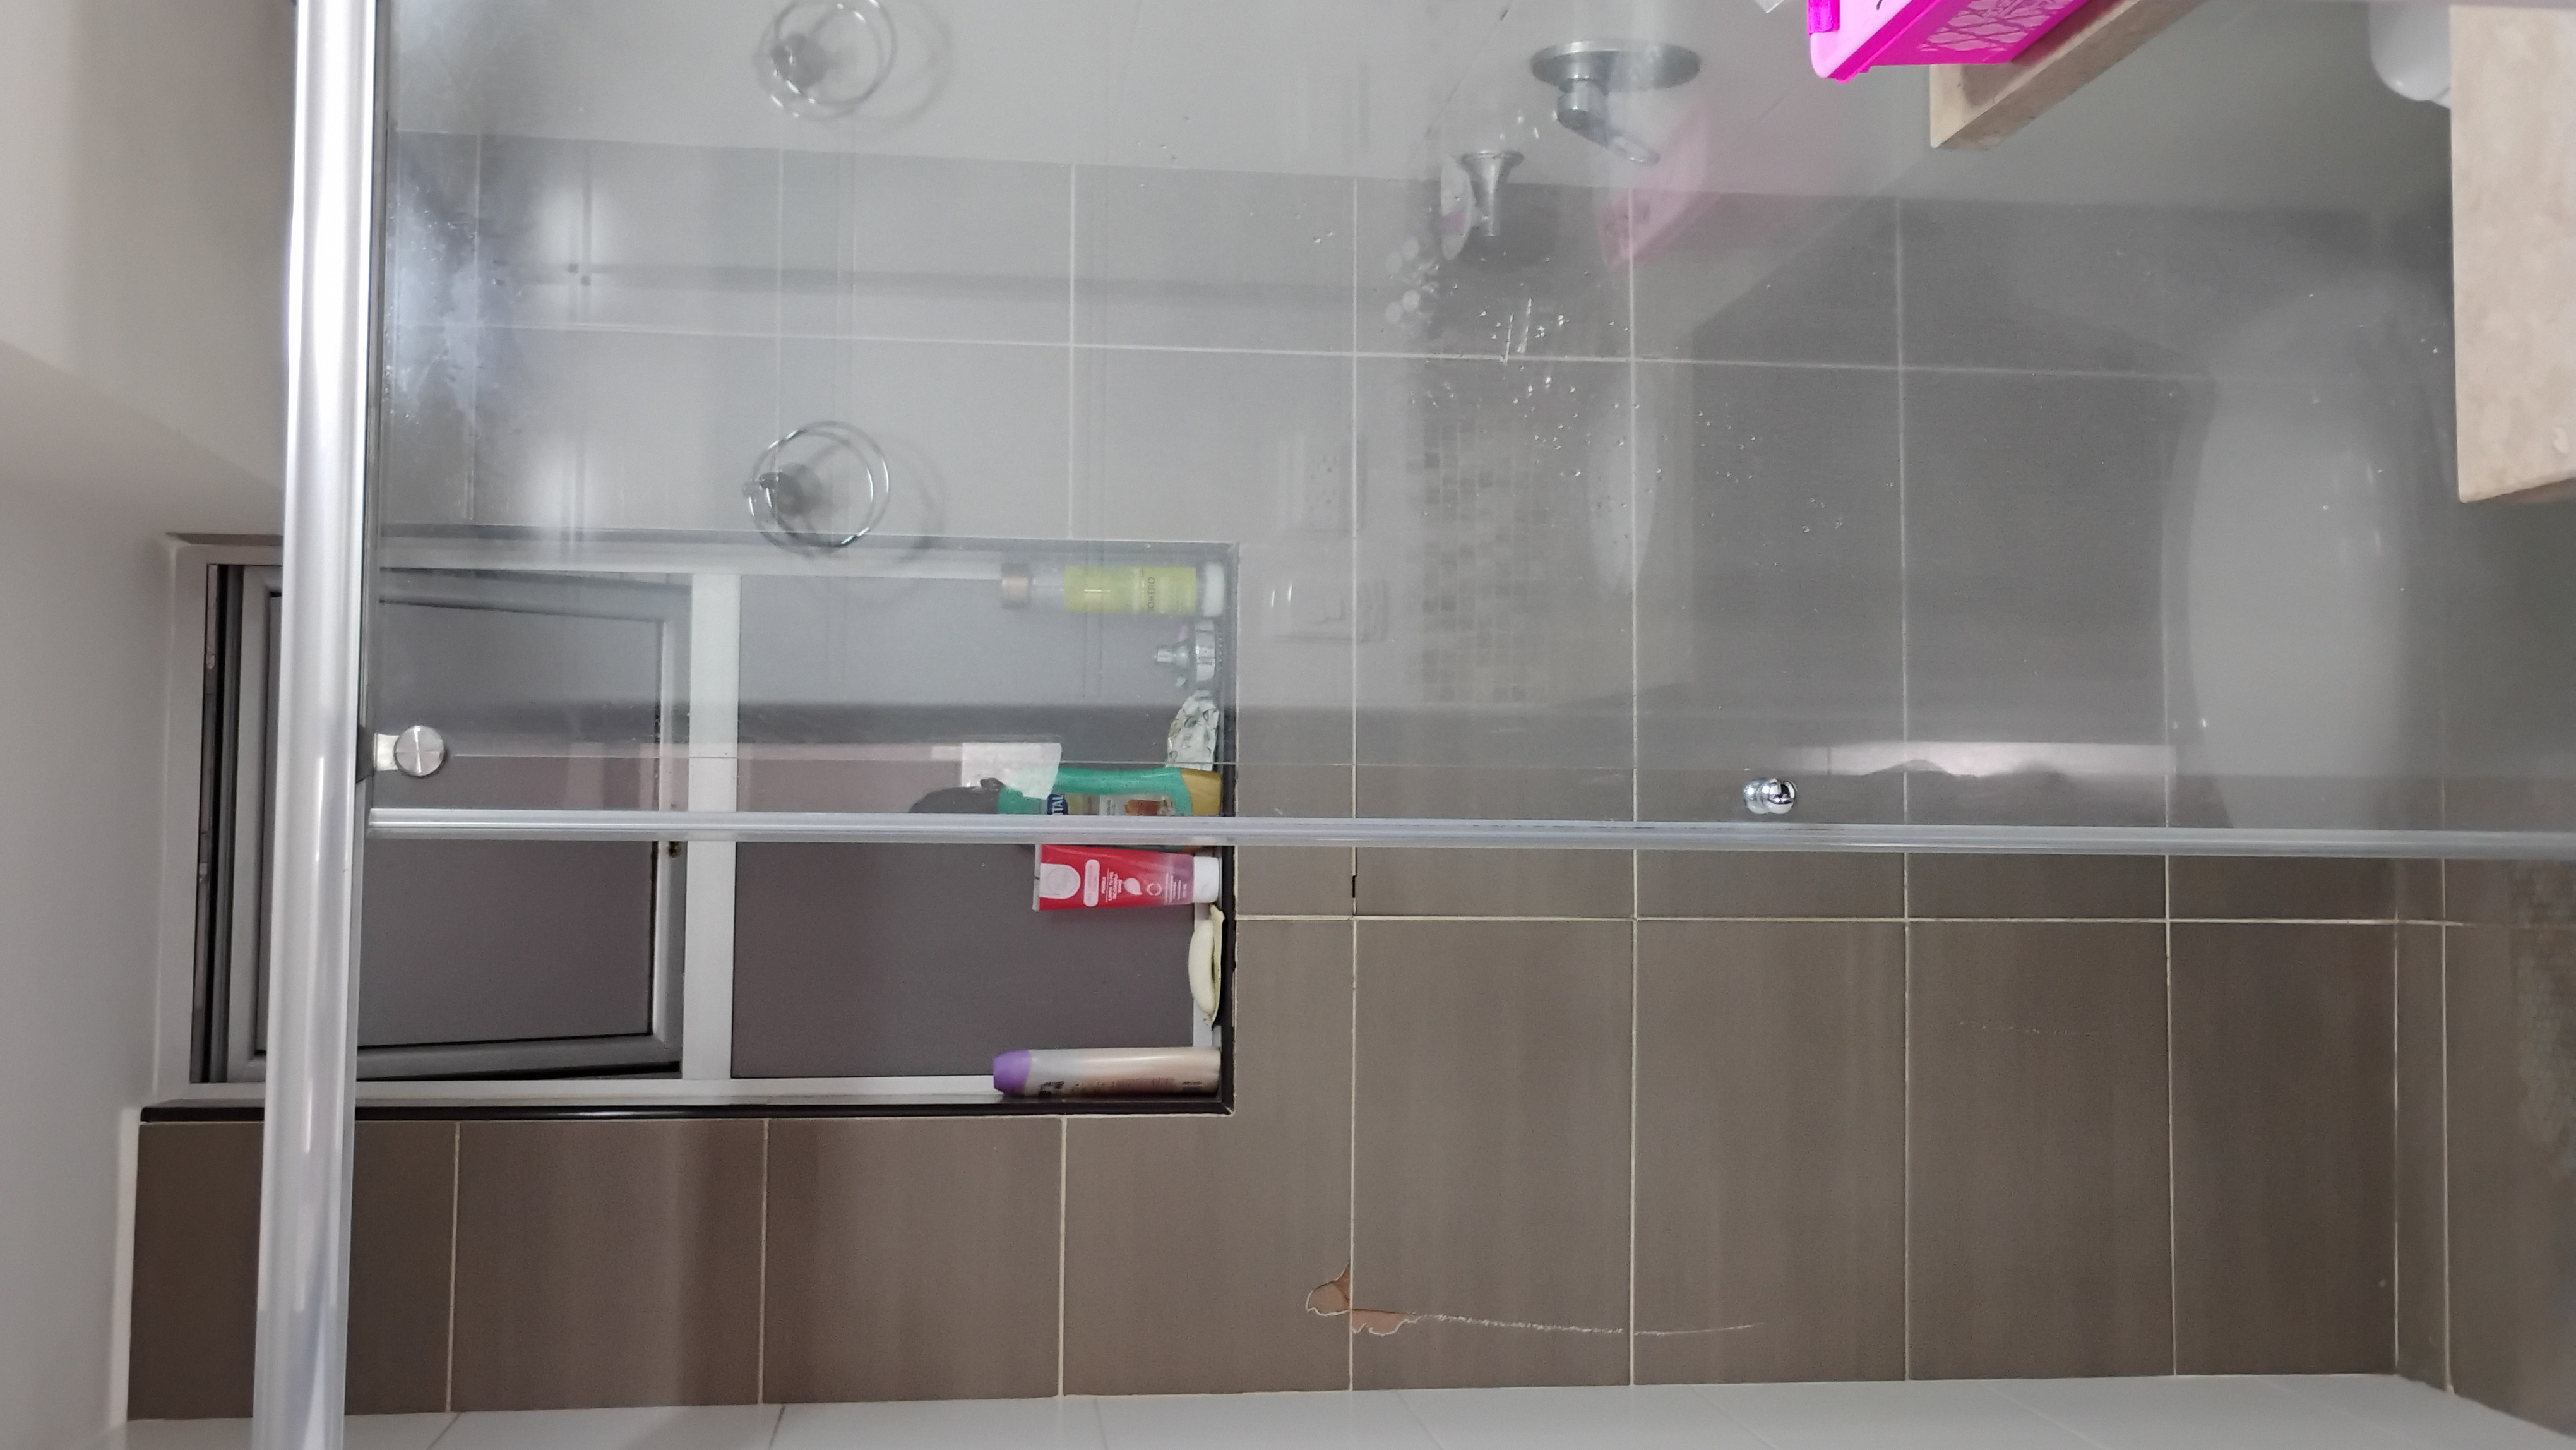
\includegraphics[width=\linewidth]{../img/IMG_20251109_150541887.jpg}\\[2pt]{\footnotesize\color{primary!60!black}Foto~31 -- 15:05:41}} & \parbox{0.45\textwidth}{\centering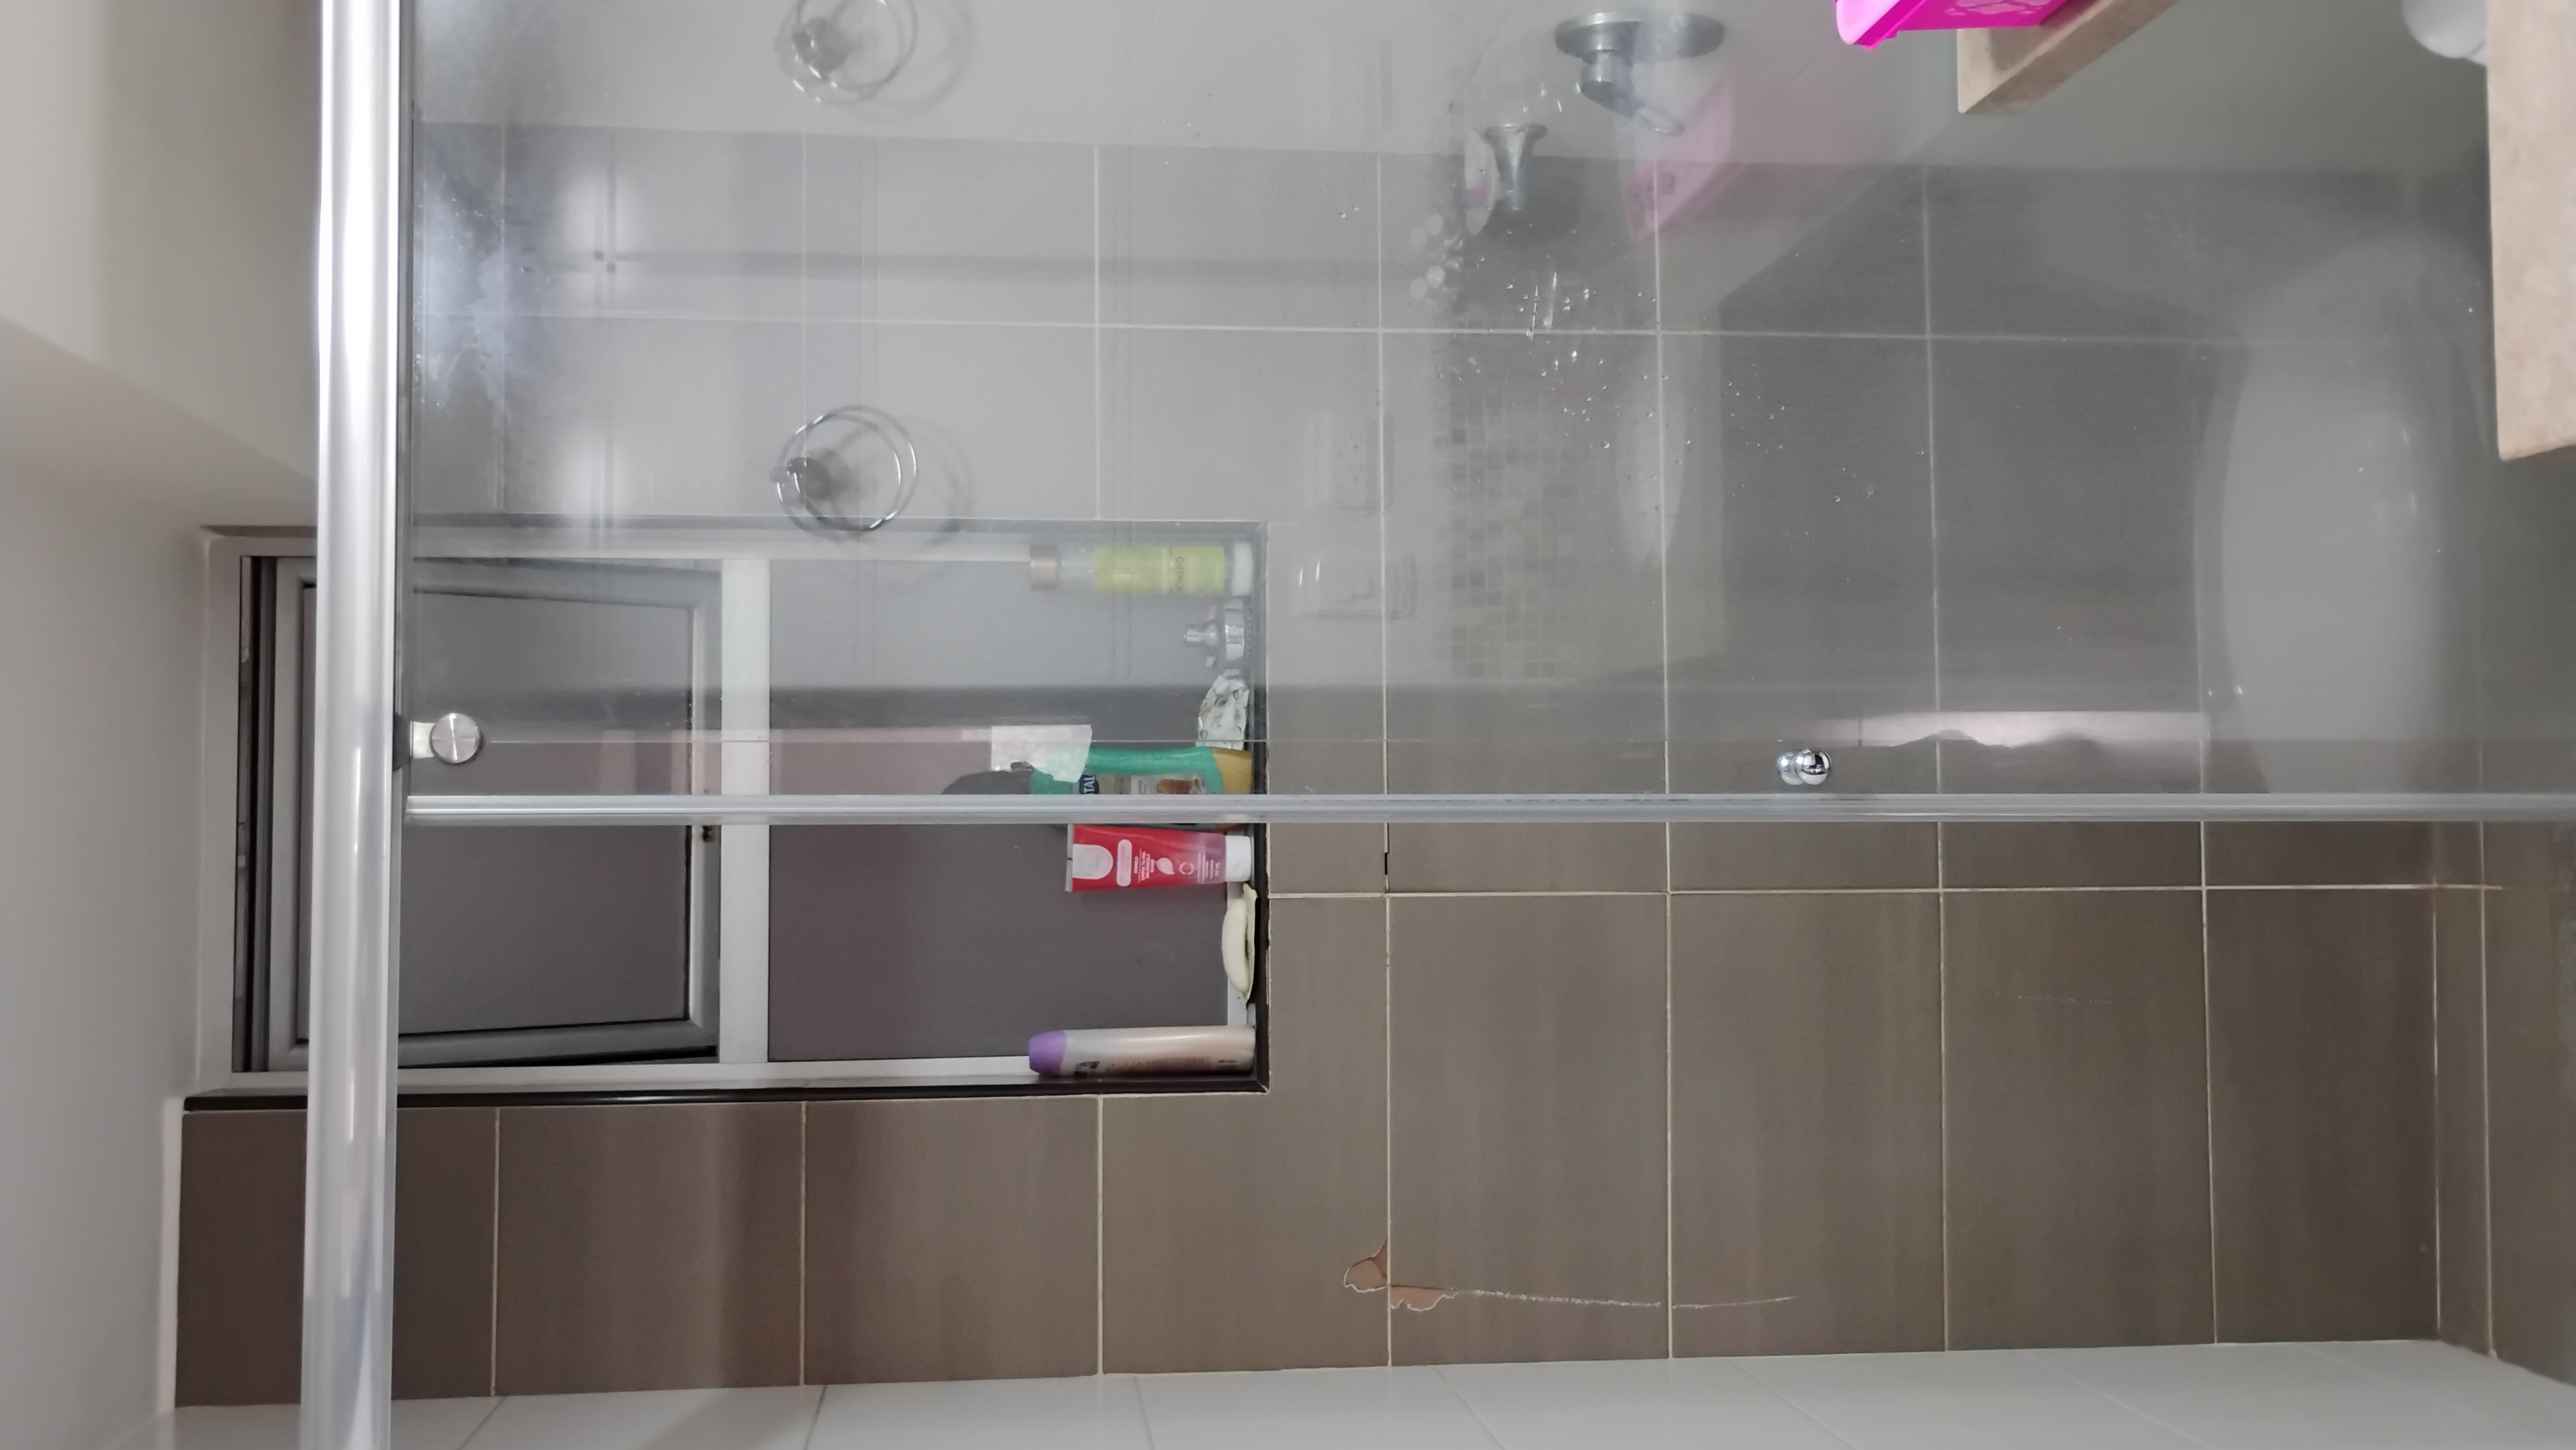
\includegraphics[width=\linewidth]{../img/IMG_20251109_150542789.jpg}\\[2pt]{\footnotesize\color{primary!60!black}Foto~32 -- 15:05:42}} \\[4pt]
\parbox{0.45\textwidth}{\centering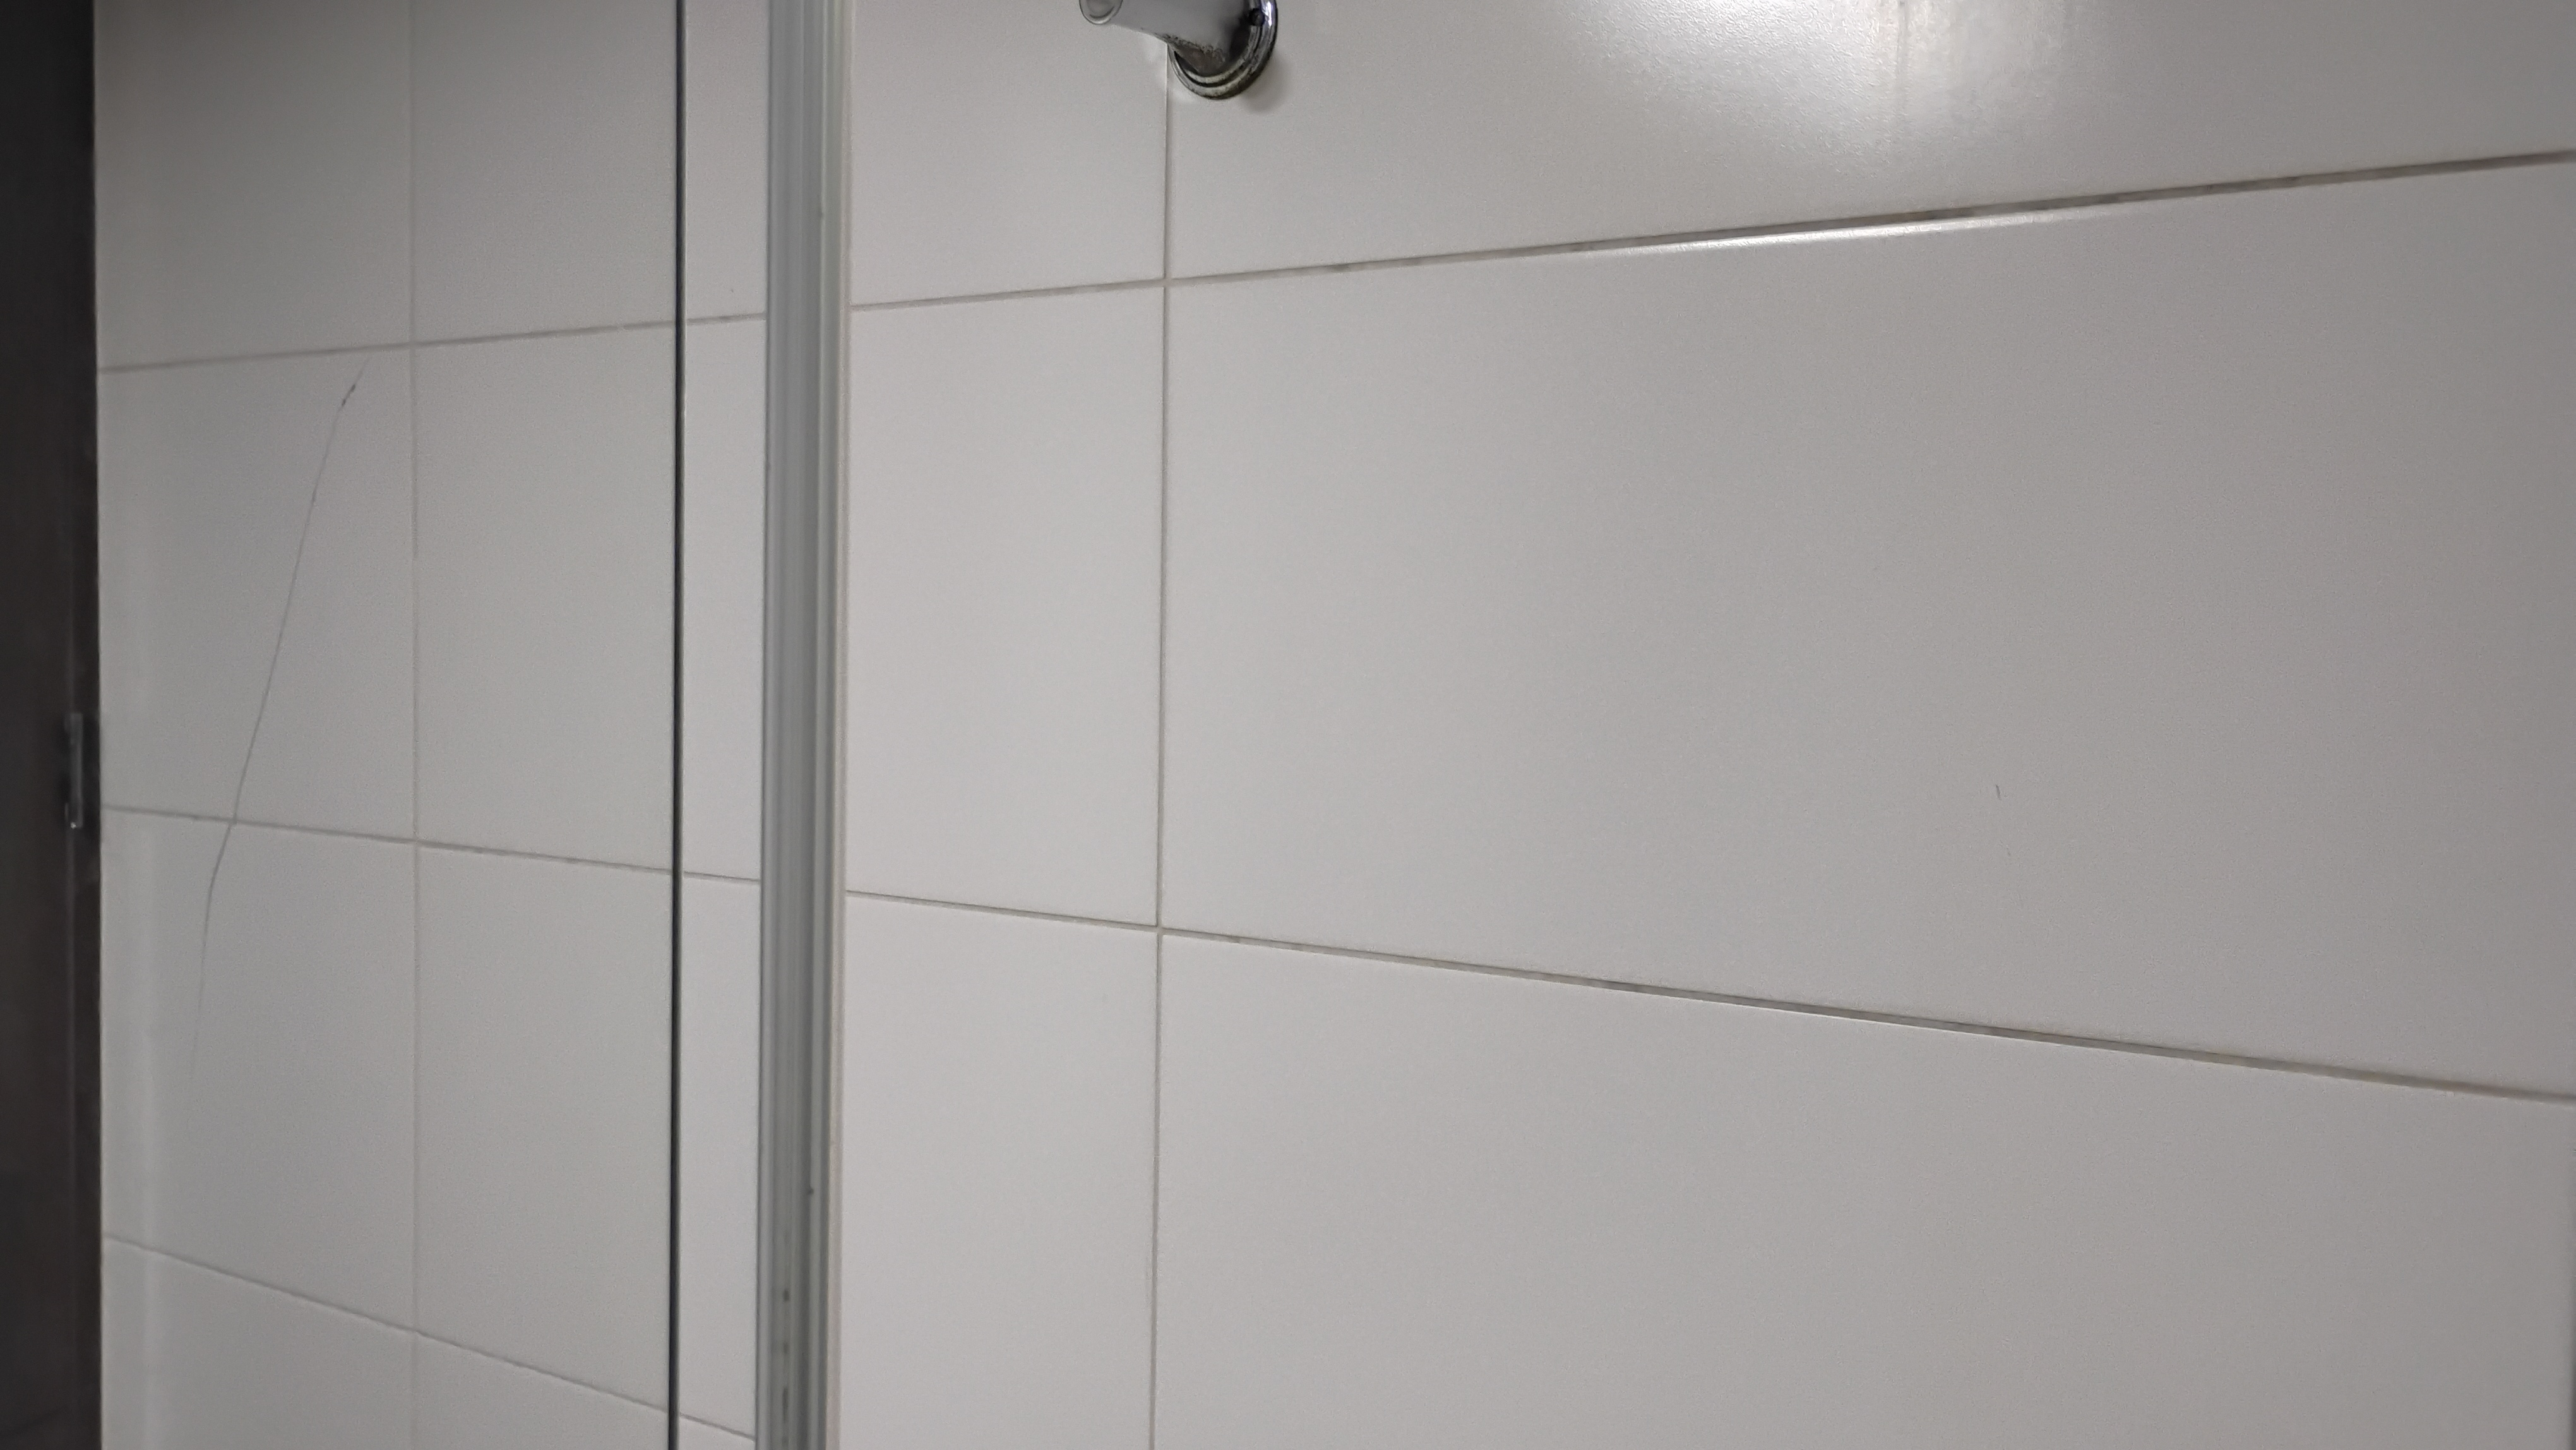
\includegraphics[width=\linewidth]{../img/IMG_20251109_150621035.jpg}\\[2pt]{\footnotesize\color{primary!60!black}Foto~33 -- 15:06:21}} & \parbox{0.45\textwidth}{\centering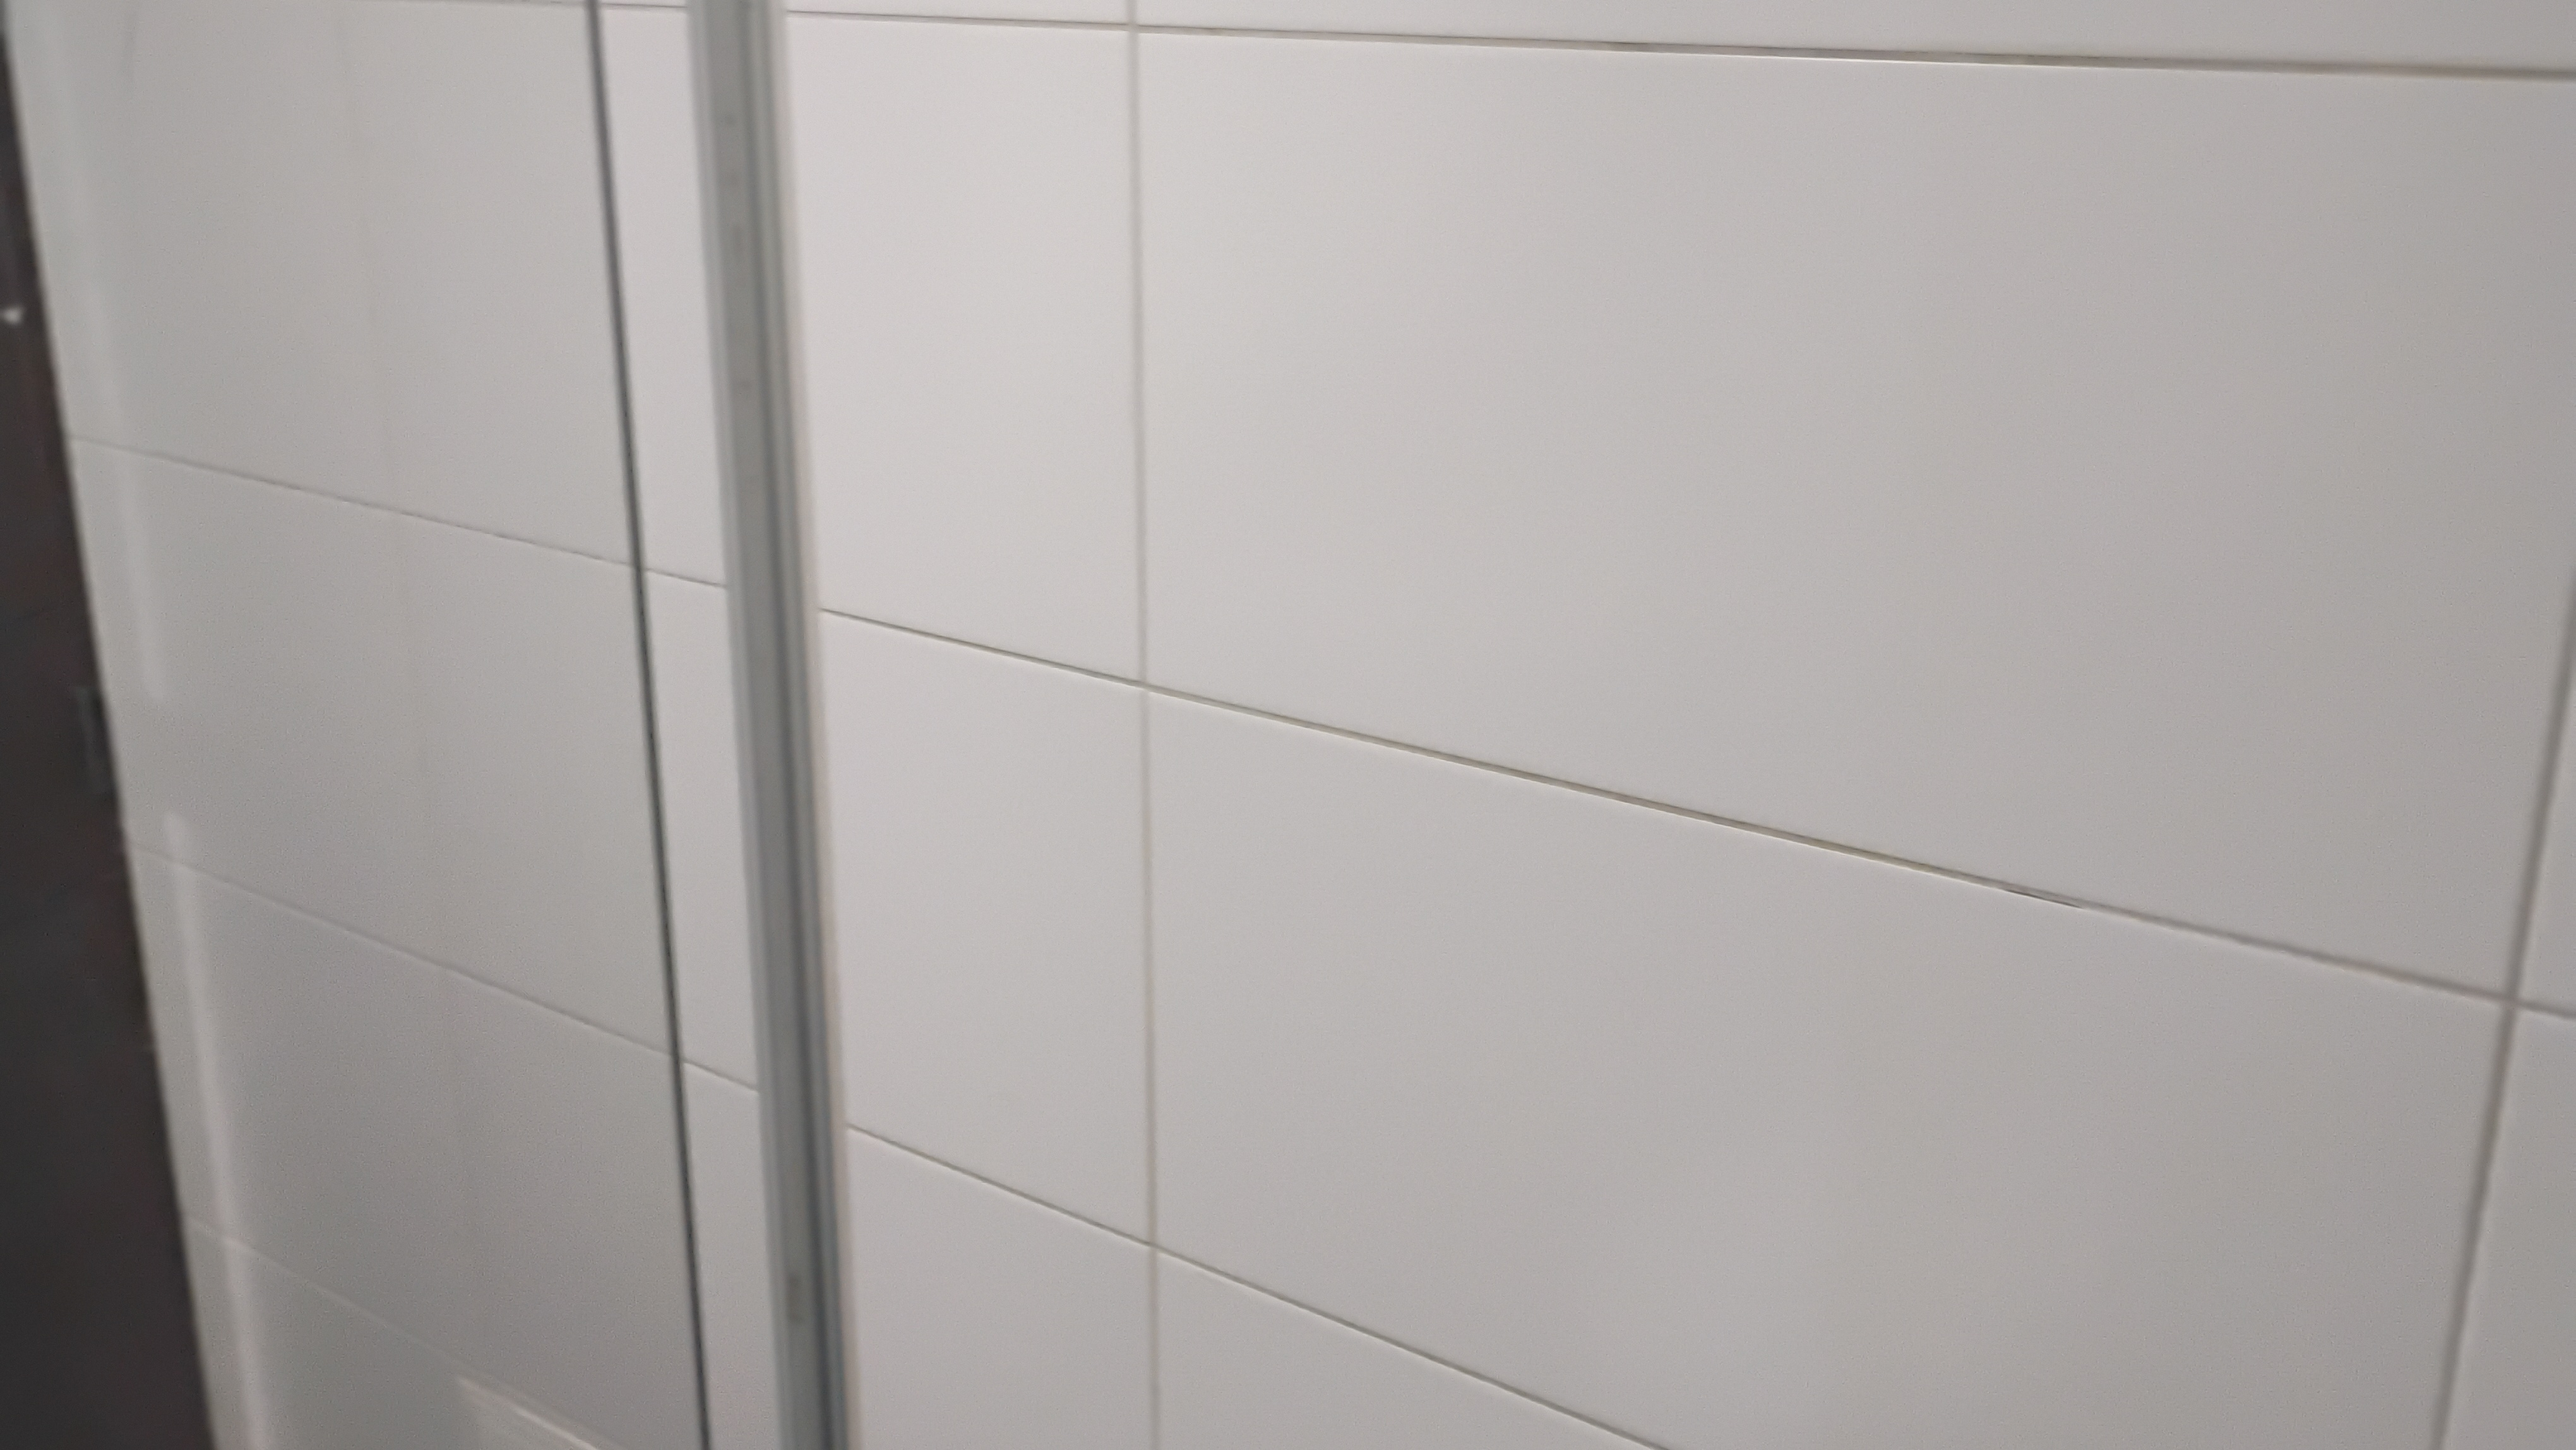
\includegraphics[width=\linewidth]{../img/IMG_20251109_150622858.jpg}\\[2pt]{\footnotesize\color{primary!60!black}Foto~34 -- 15:06:22}} \\[4pt]
\parbox{0.45\textwidth}{\centering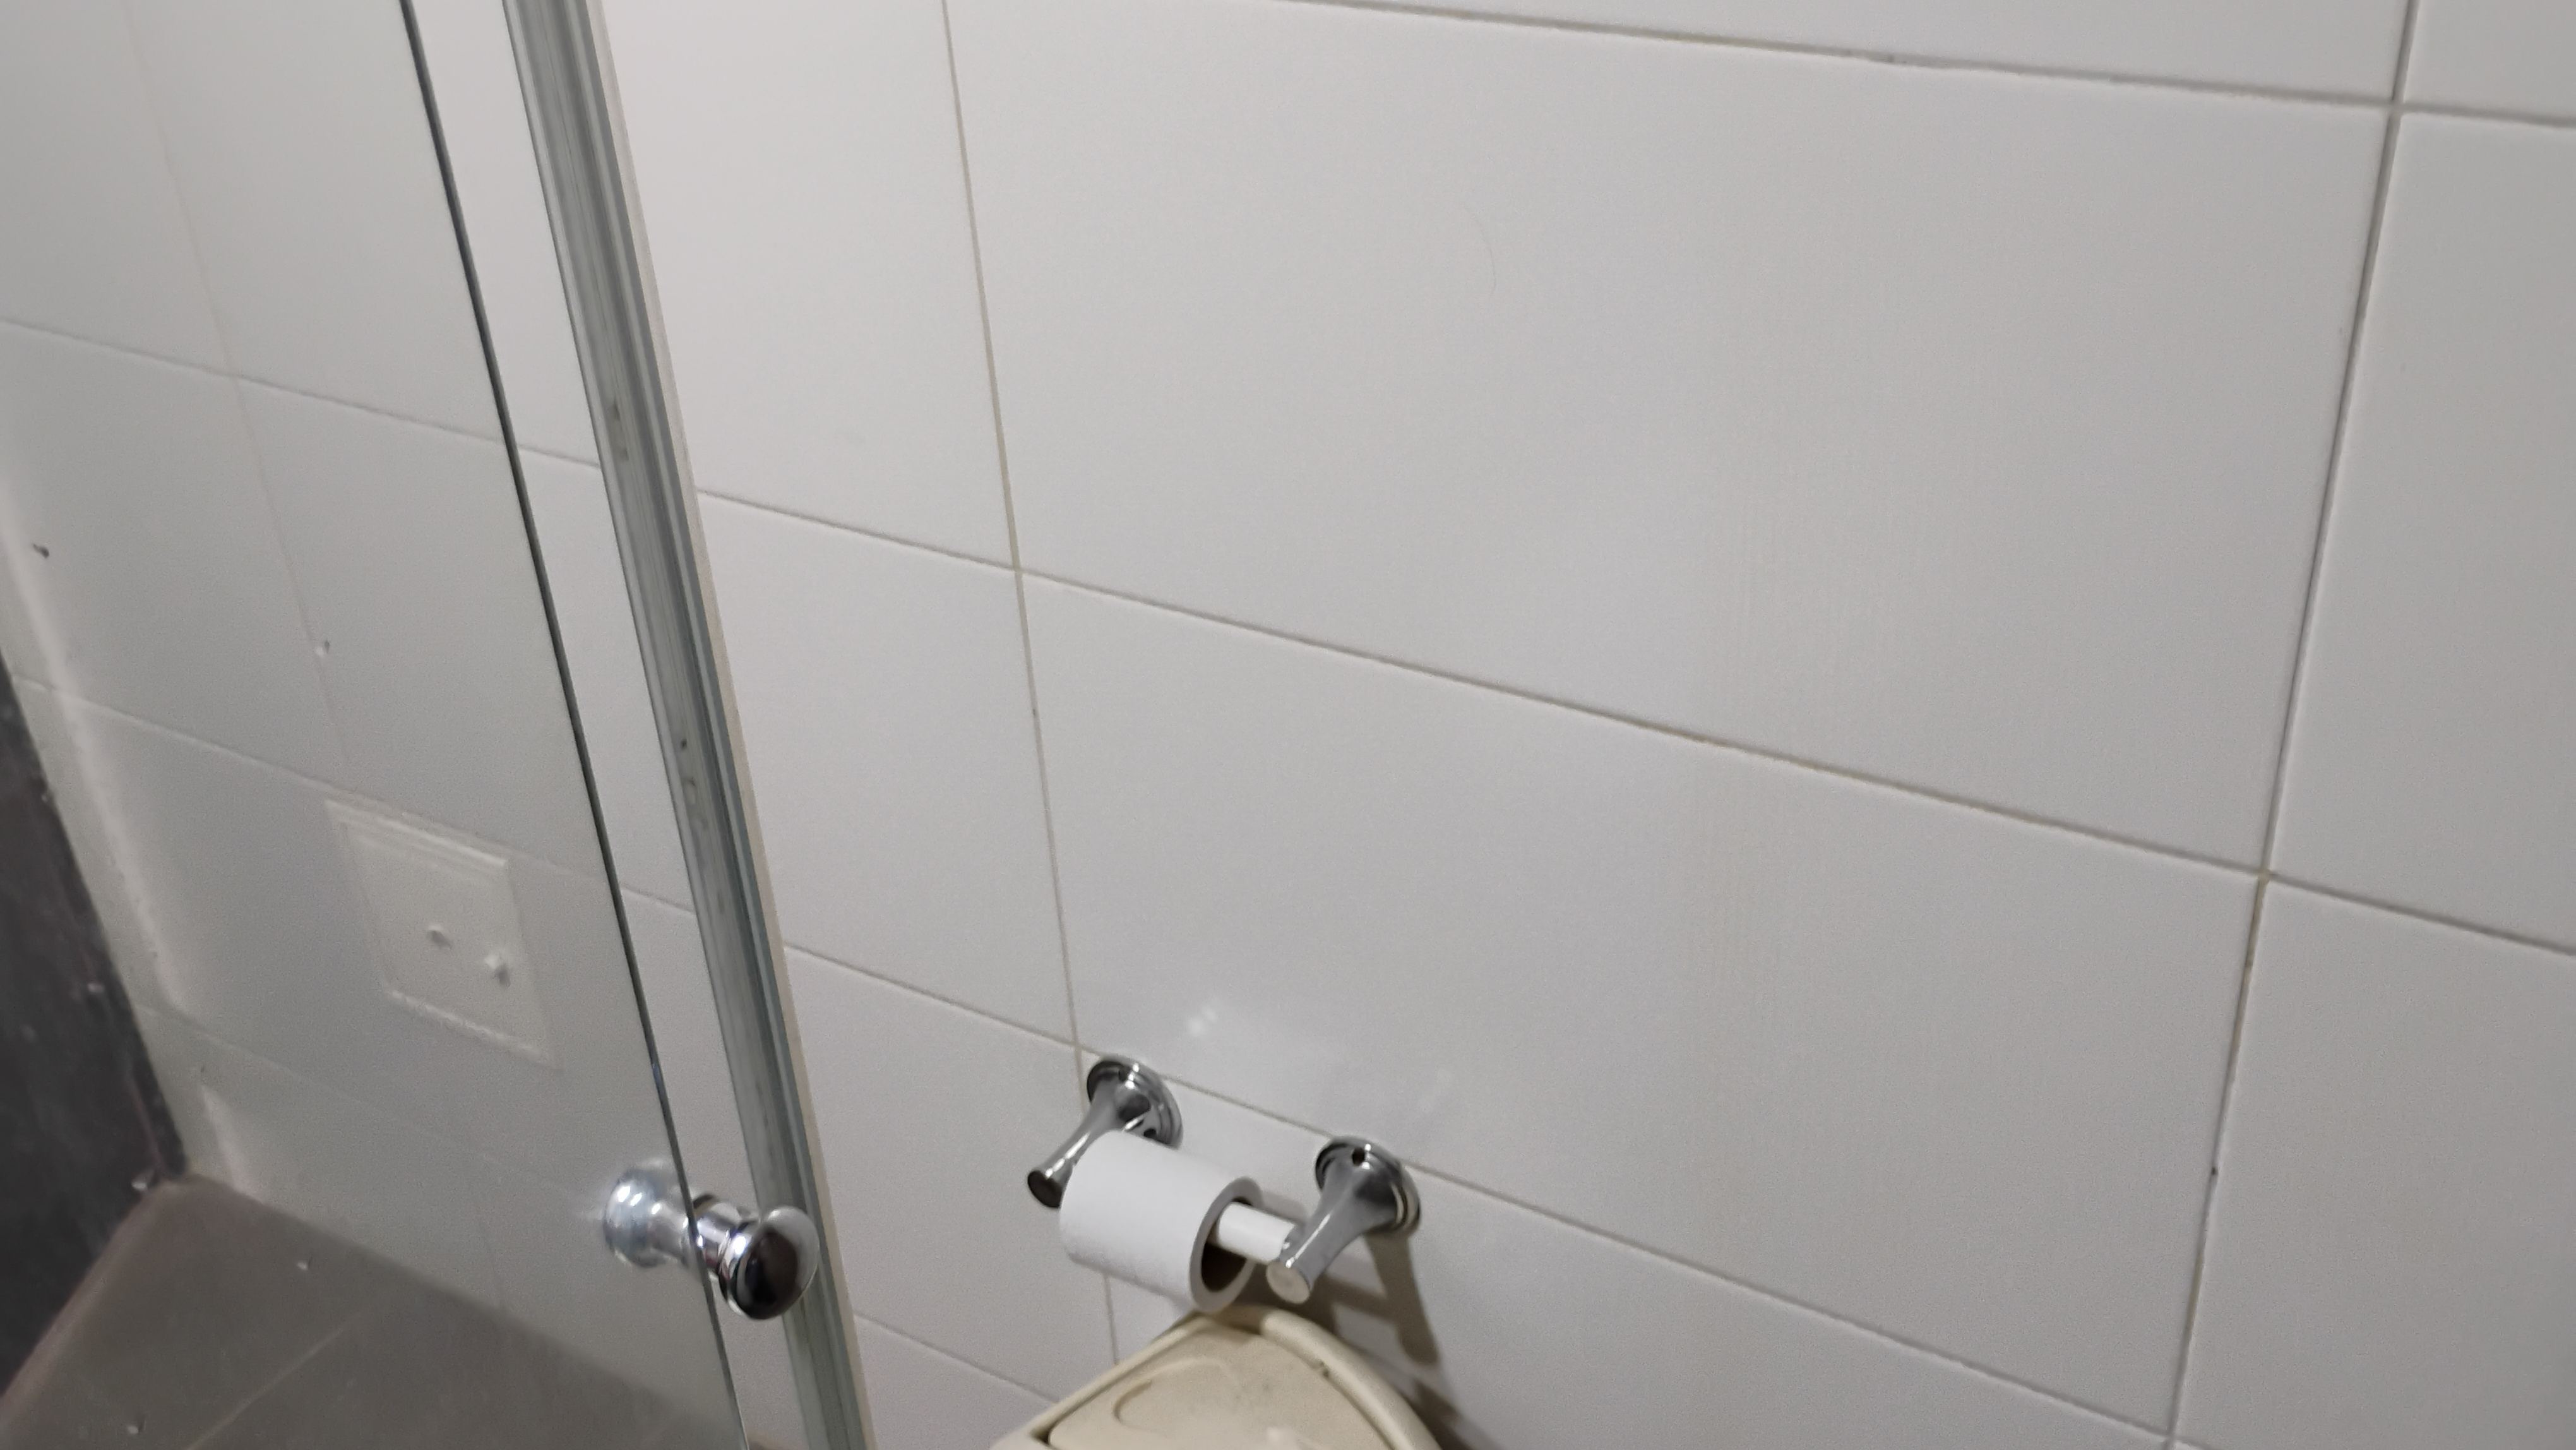
\includegraphics[width=\linewidth]{../img/IMG_20251109_150624605.jpg}\\[2pt]{\footnotesize\color{primary!60!black}Foto~35 -- 15:06:24}} & \parbox{0.45\textwidth}{\centering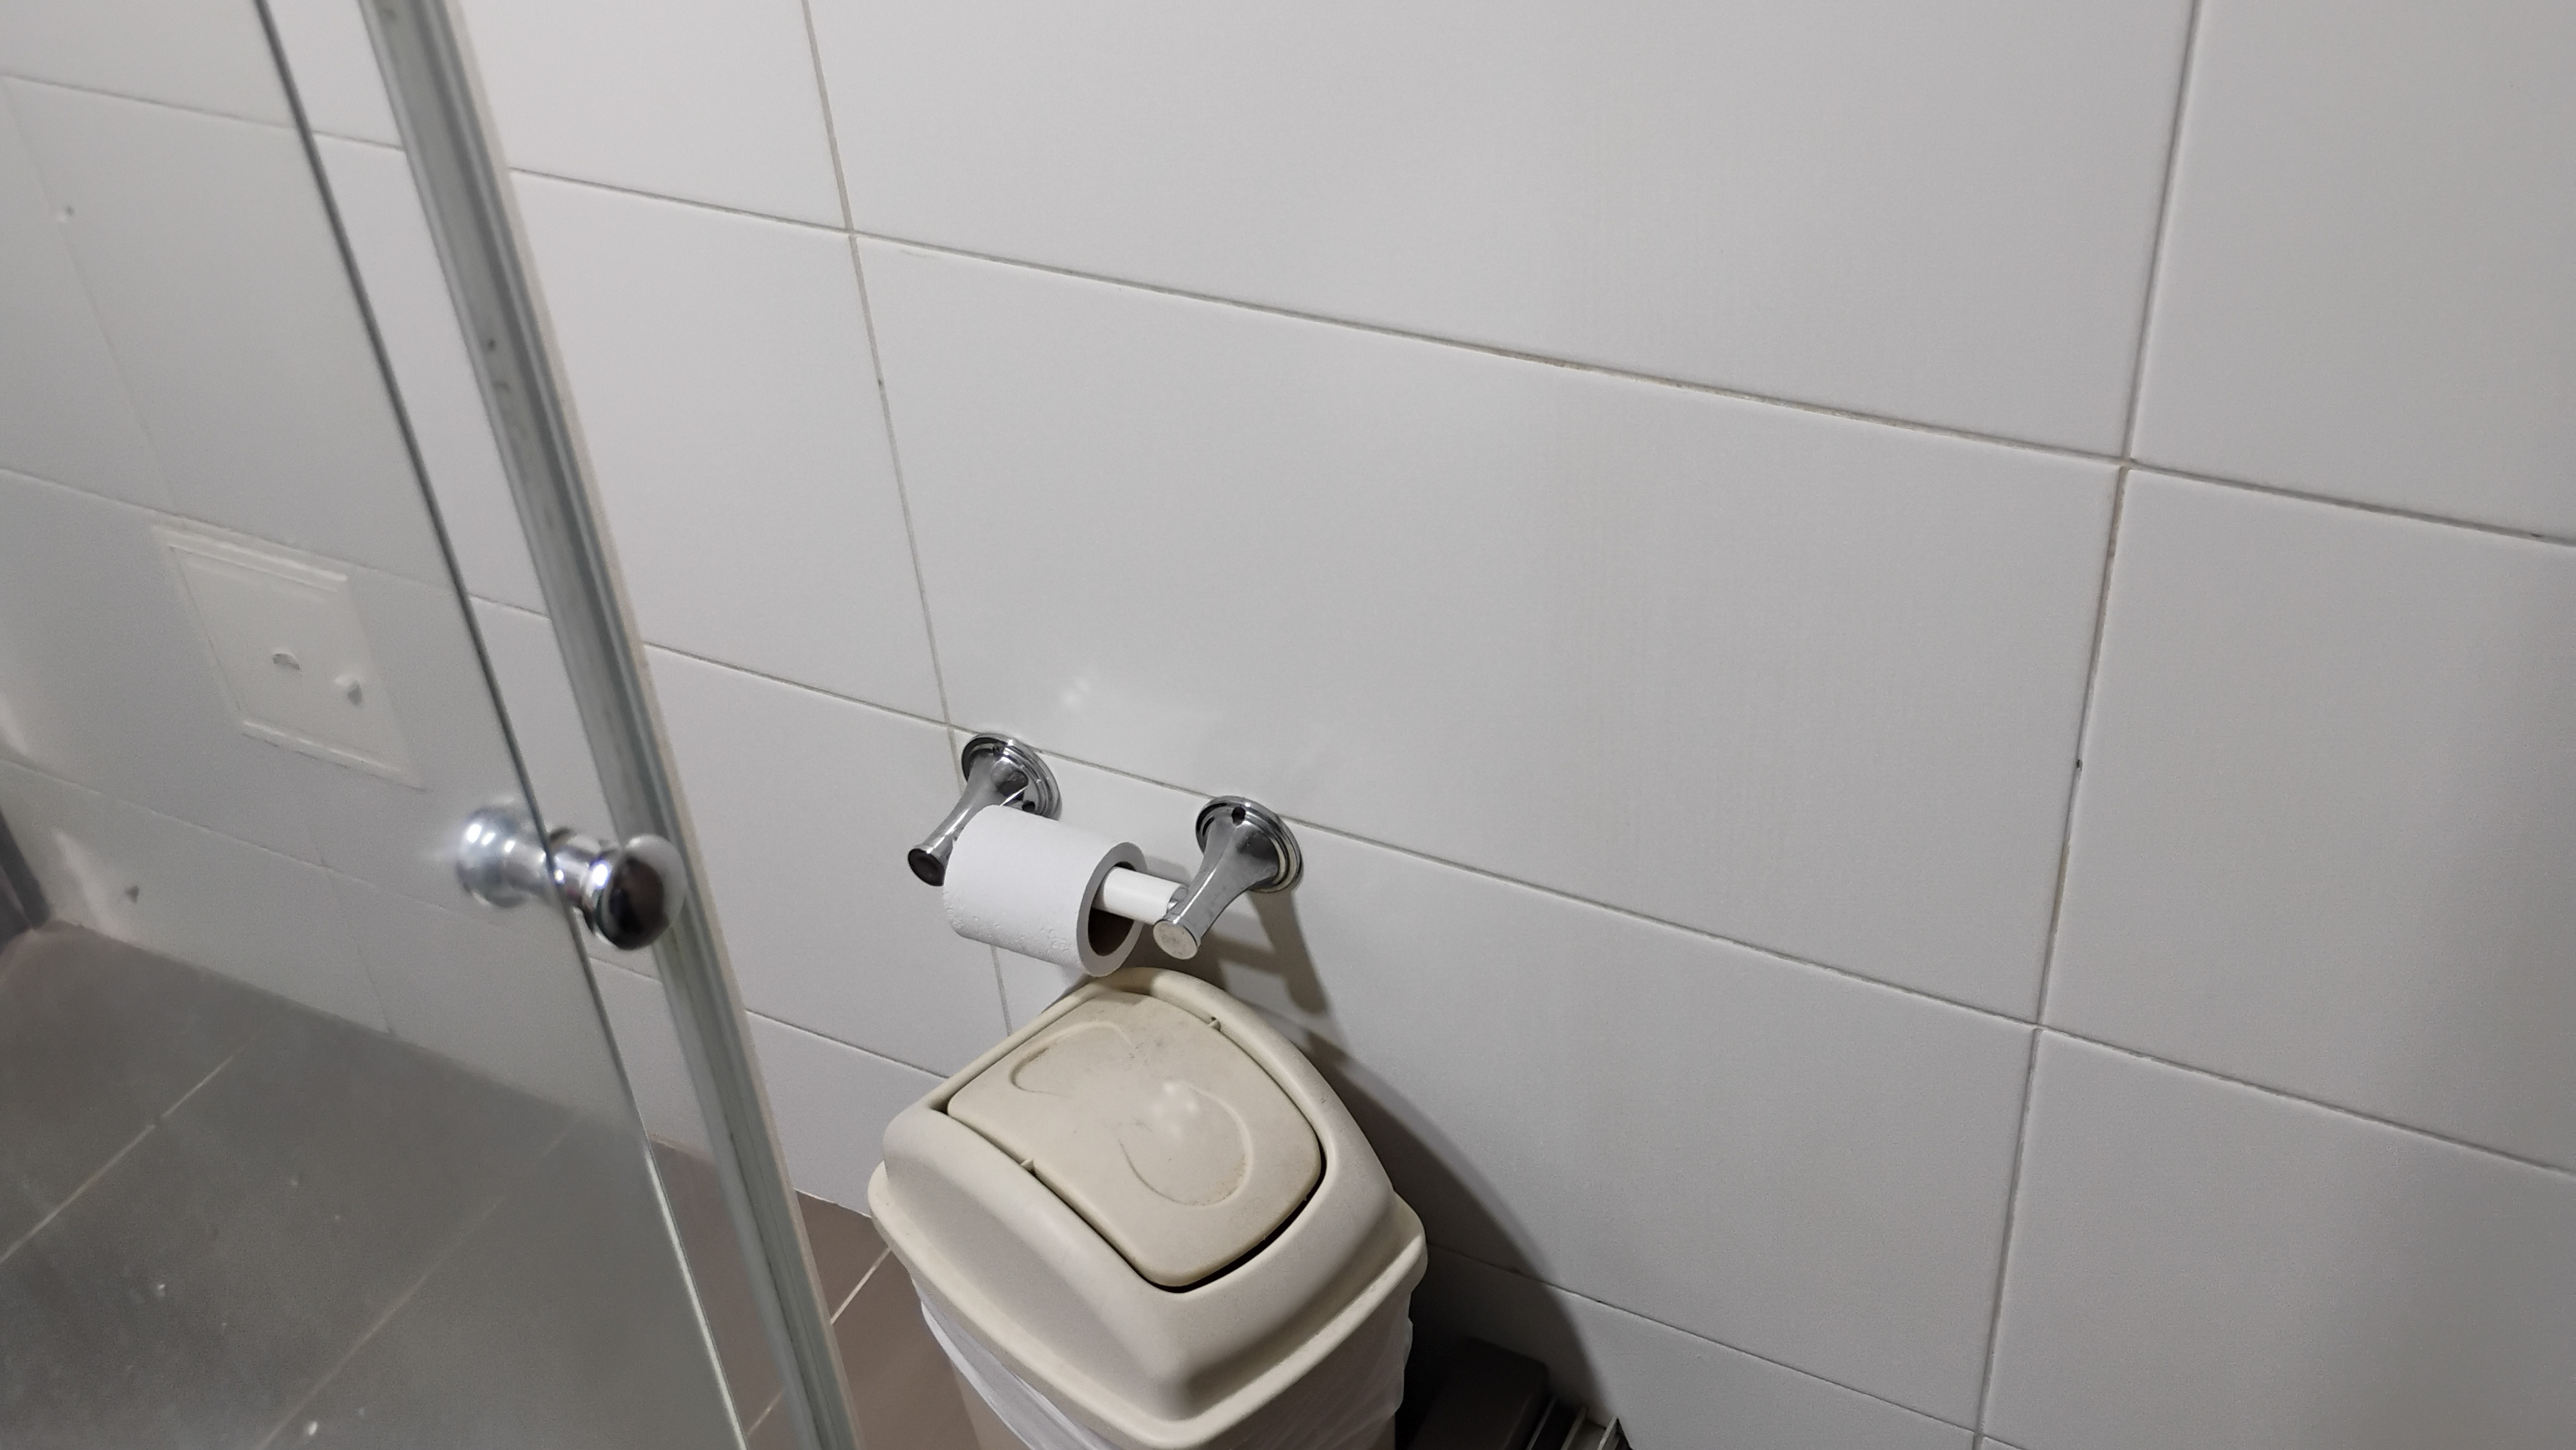
\includegraphics[width=\linewidth]{../img/IMG_20251109_150626192.jpg}\\[2pt]{\footnotesize\color{primary!60!black}Foto~36 -- 15:06:26}} \\[4pt]
\end{tabular}
\caption{Zona de Ducha — Filtración y Eflorescencia Salina: Fotos 31 al 36.}\end{figure}
\newpage
\begin{figure}[H]
\centering
\begin{tabular}{cc}
\parbox{0.45\textwidth}{\centering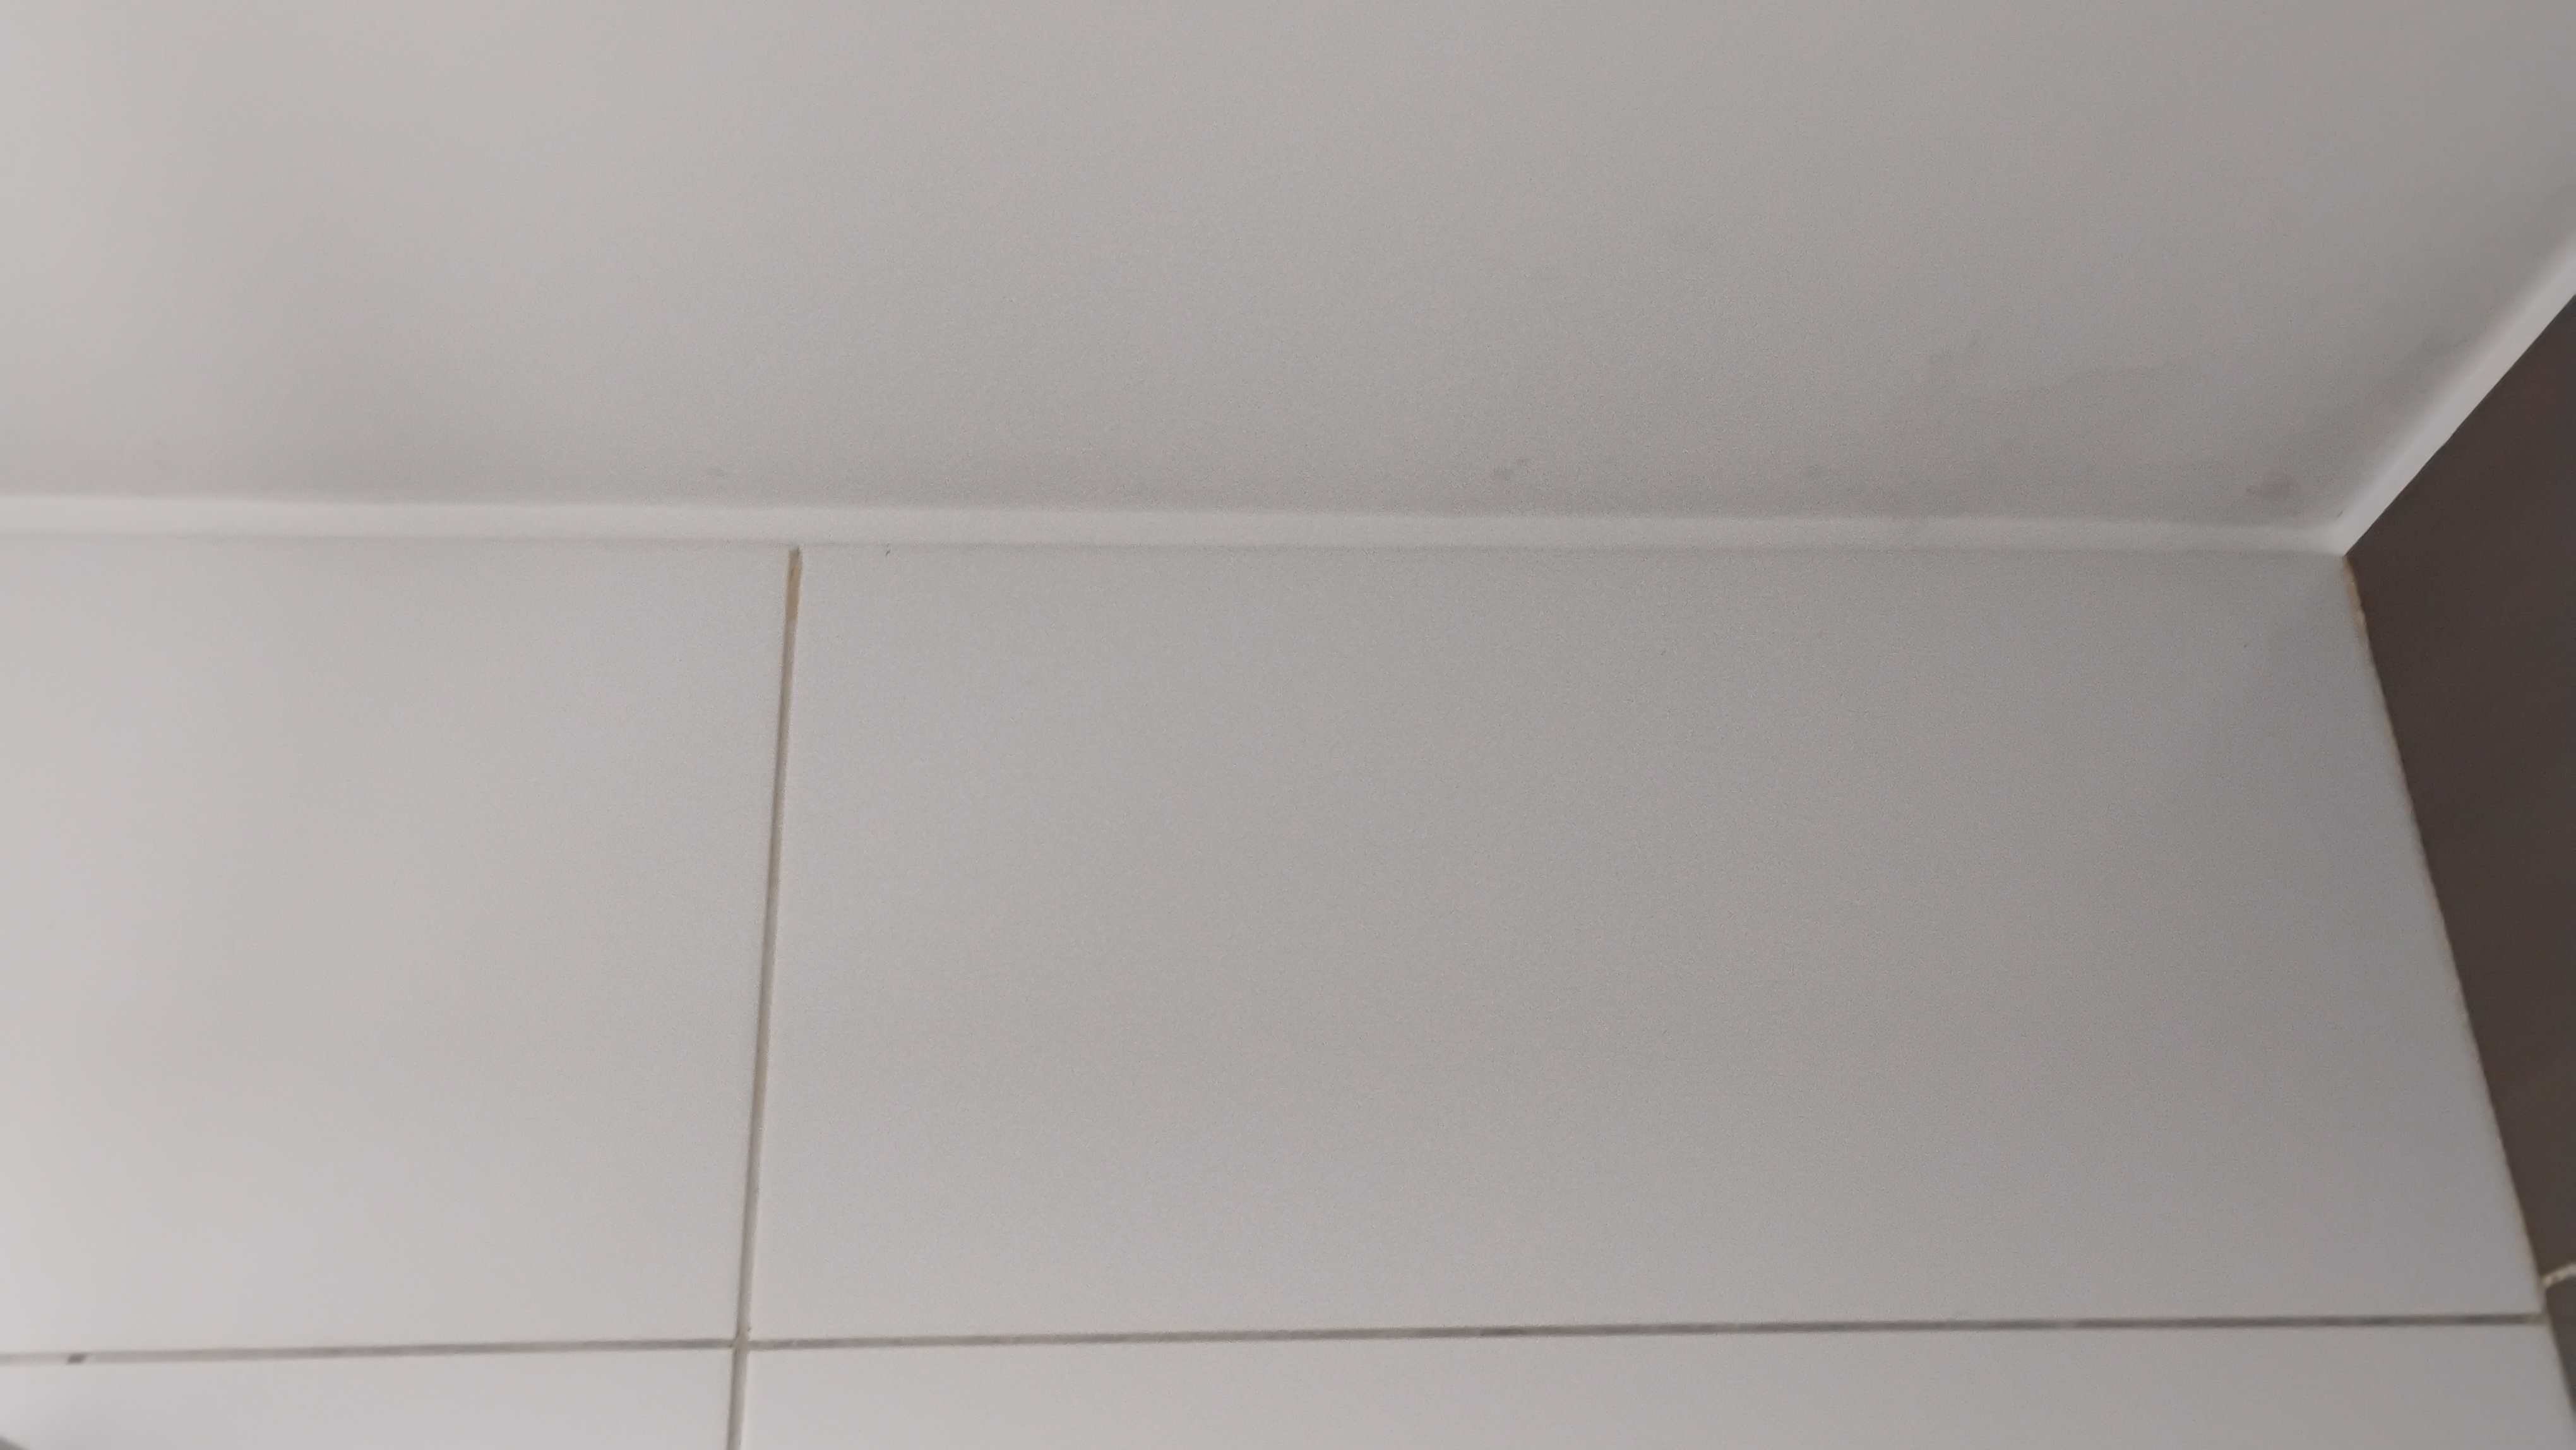
\includegraphics[width=\linewidth]{../img/IMG_20251109_150630153.jpg}\\[2pt]{\footnotesize\color{primary!60!black}Foto~37 -- 15:06:30}} & \parbox{0.45\textwidth}{\centering
\includegraphics[width=\linewidth]{../img/IMG_20251109_150634089.jpg}\\[2pt]{\footnotesize\color{primary!60!black}Foto~38 -- 15:06:34}} \\[4pt]
\parbox{0.45\textwidth}{\centering
\includegraphics[width=\linewidth]{../img/IMG_20251109_150635317.jpg}\\[2pt]{\footnotesize\color{primary!60!black}Foto~39 -- 15:06:35}} & \parbox{0.45\textwidth}{\centering
\includegraphics[width=\linewidth]{../img/IMG_20251109_150636815.jpg}\\[2pt]{\footnotesize\color{primary!60!black}Foto~40 -- 15:06:36}} \\[4pt]
\parbox{0.45\textwidth}{\centering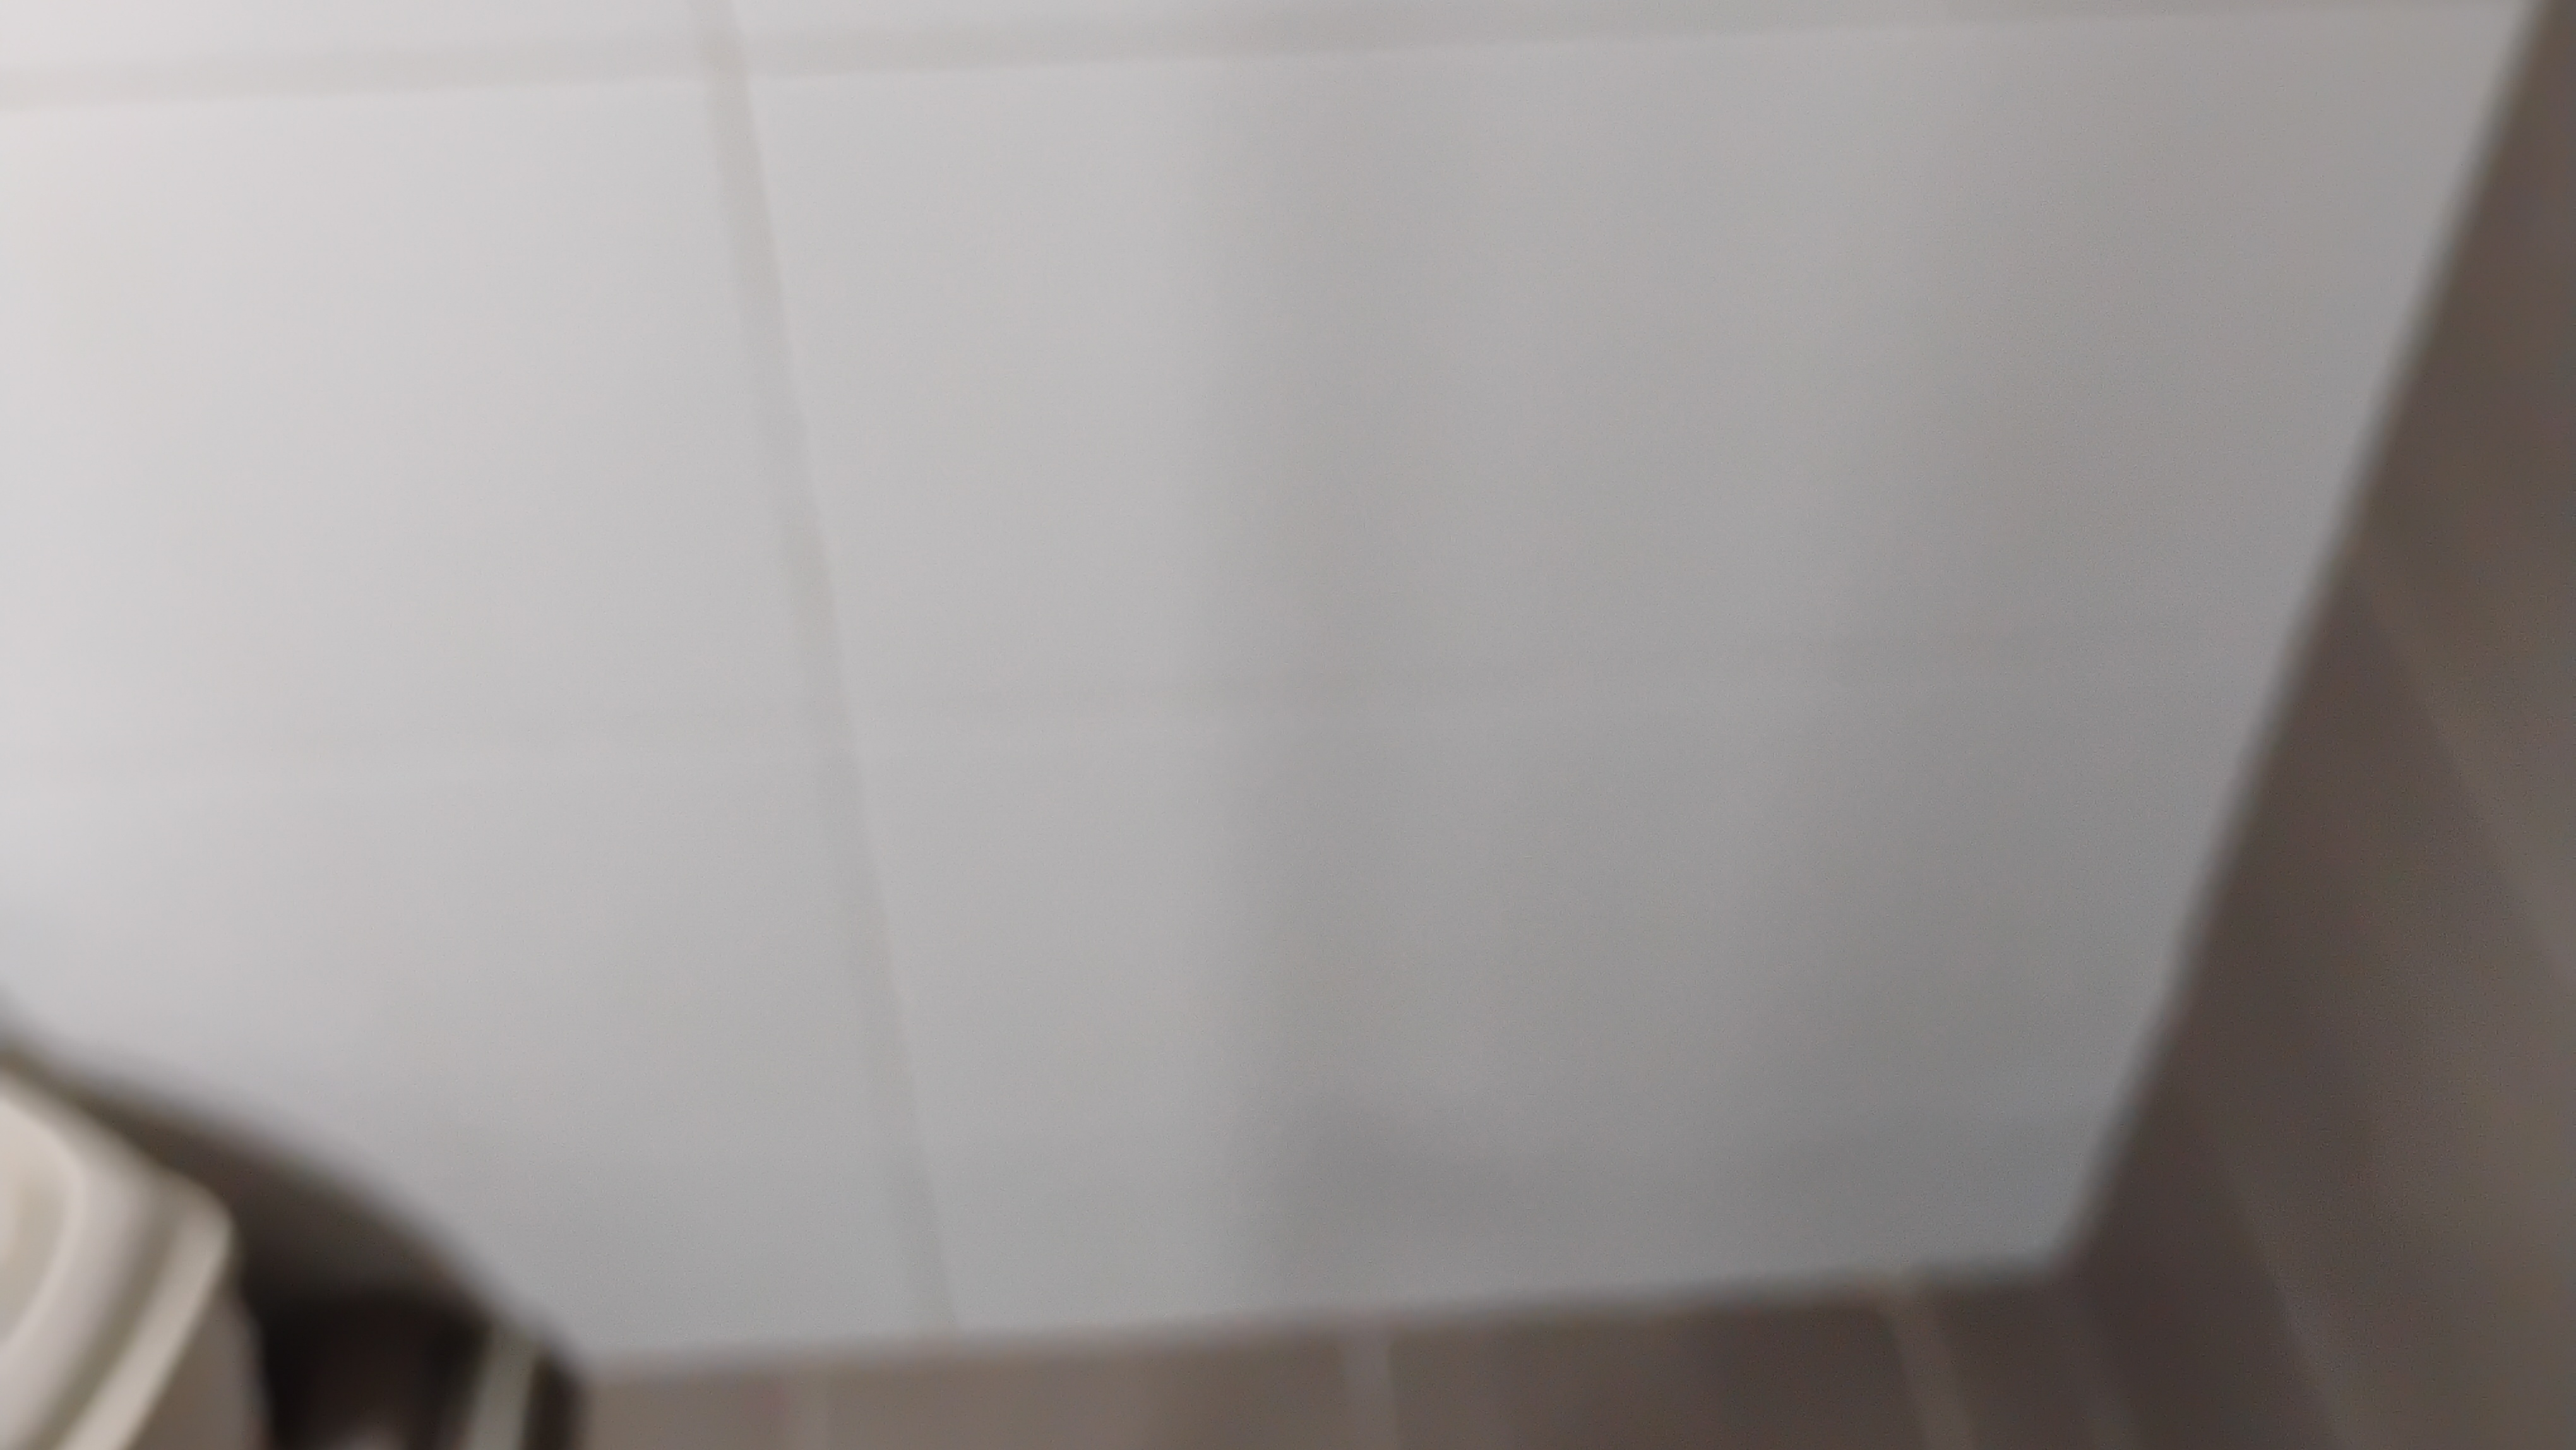
\includegraphics[width=\linewidth]{../img/IMG_20251109_150638232.jpg}\\[2pt]{\footnotesize\color{primary!60!black}Foto~41 -- 15:06:38}} & \parbox{0.45\textwidth}{\centering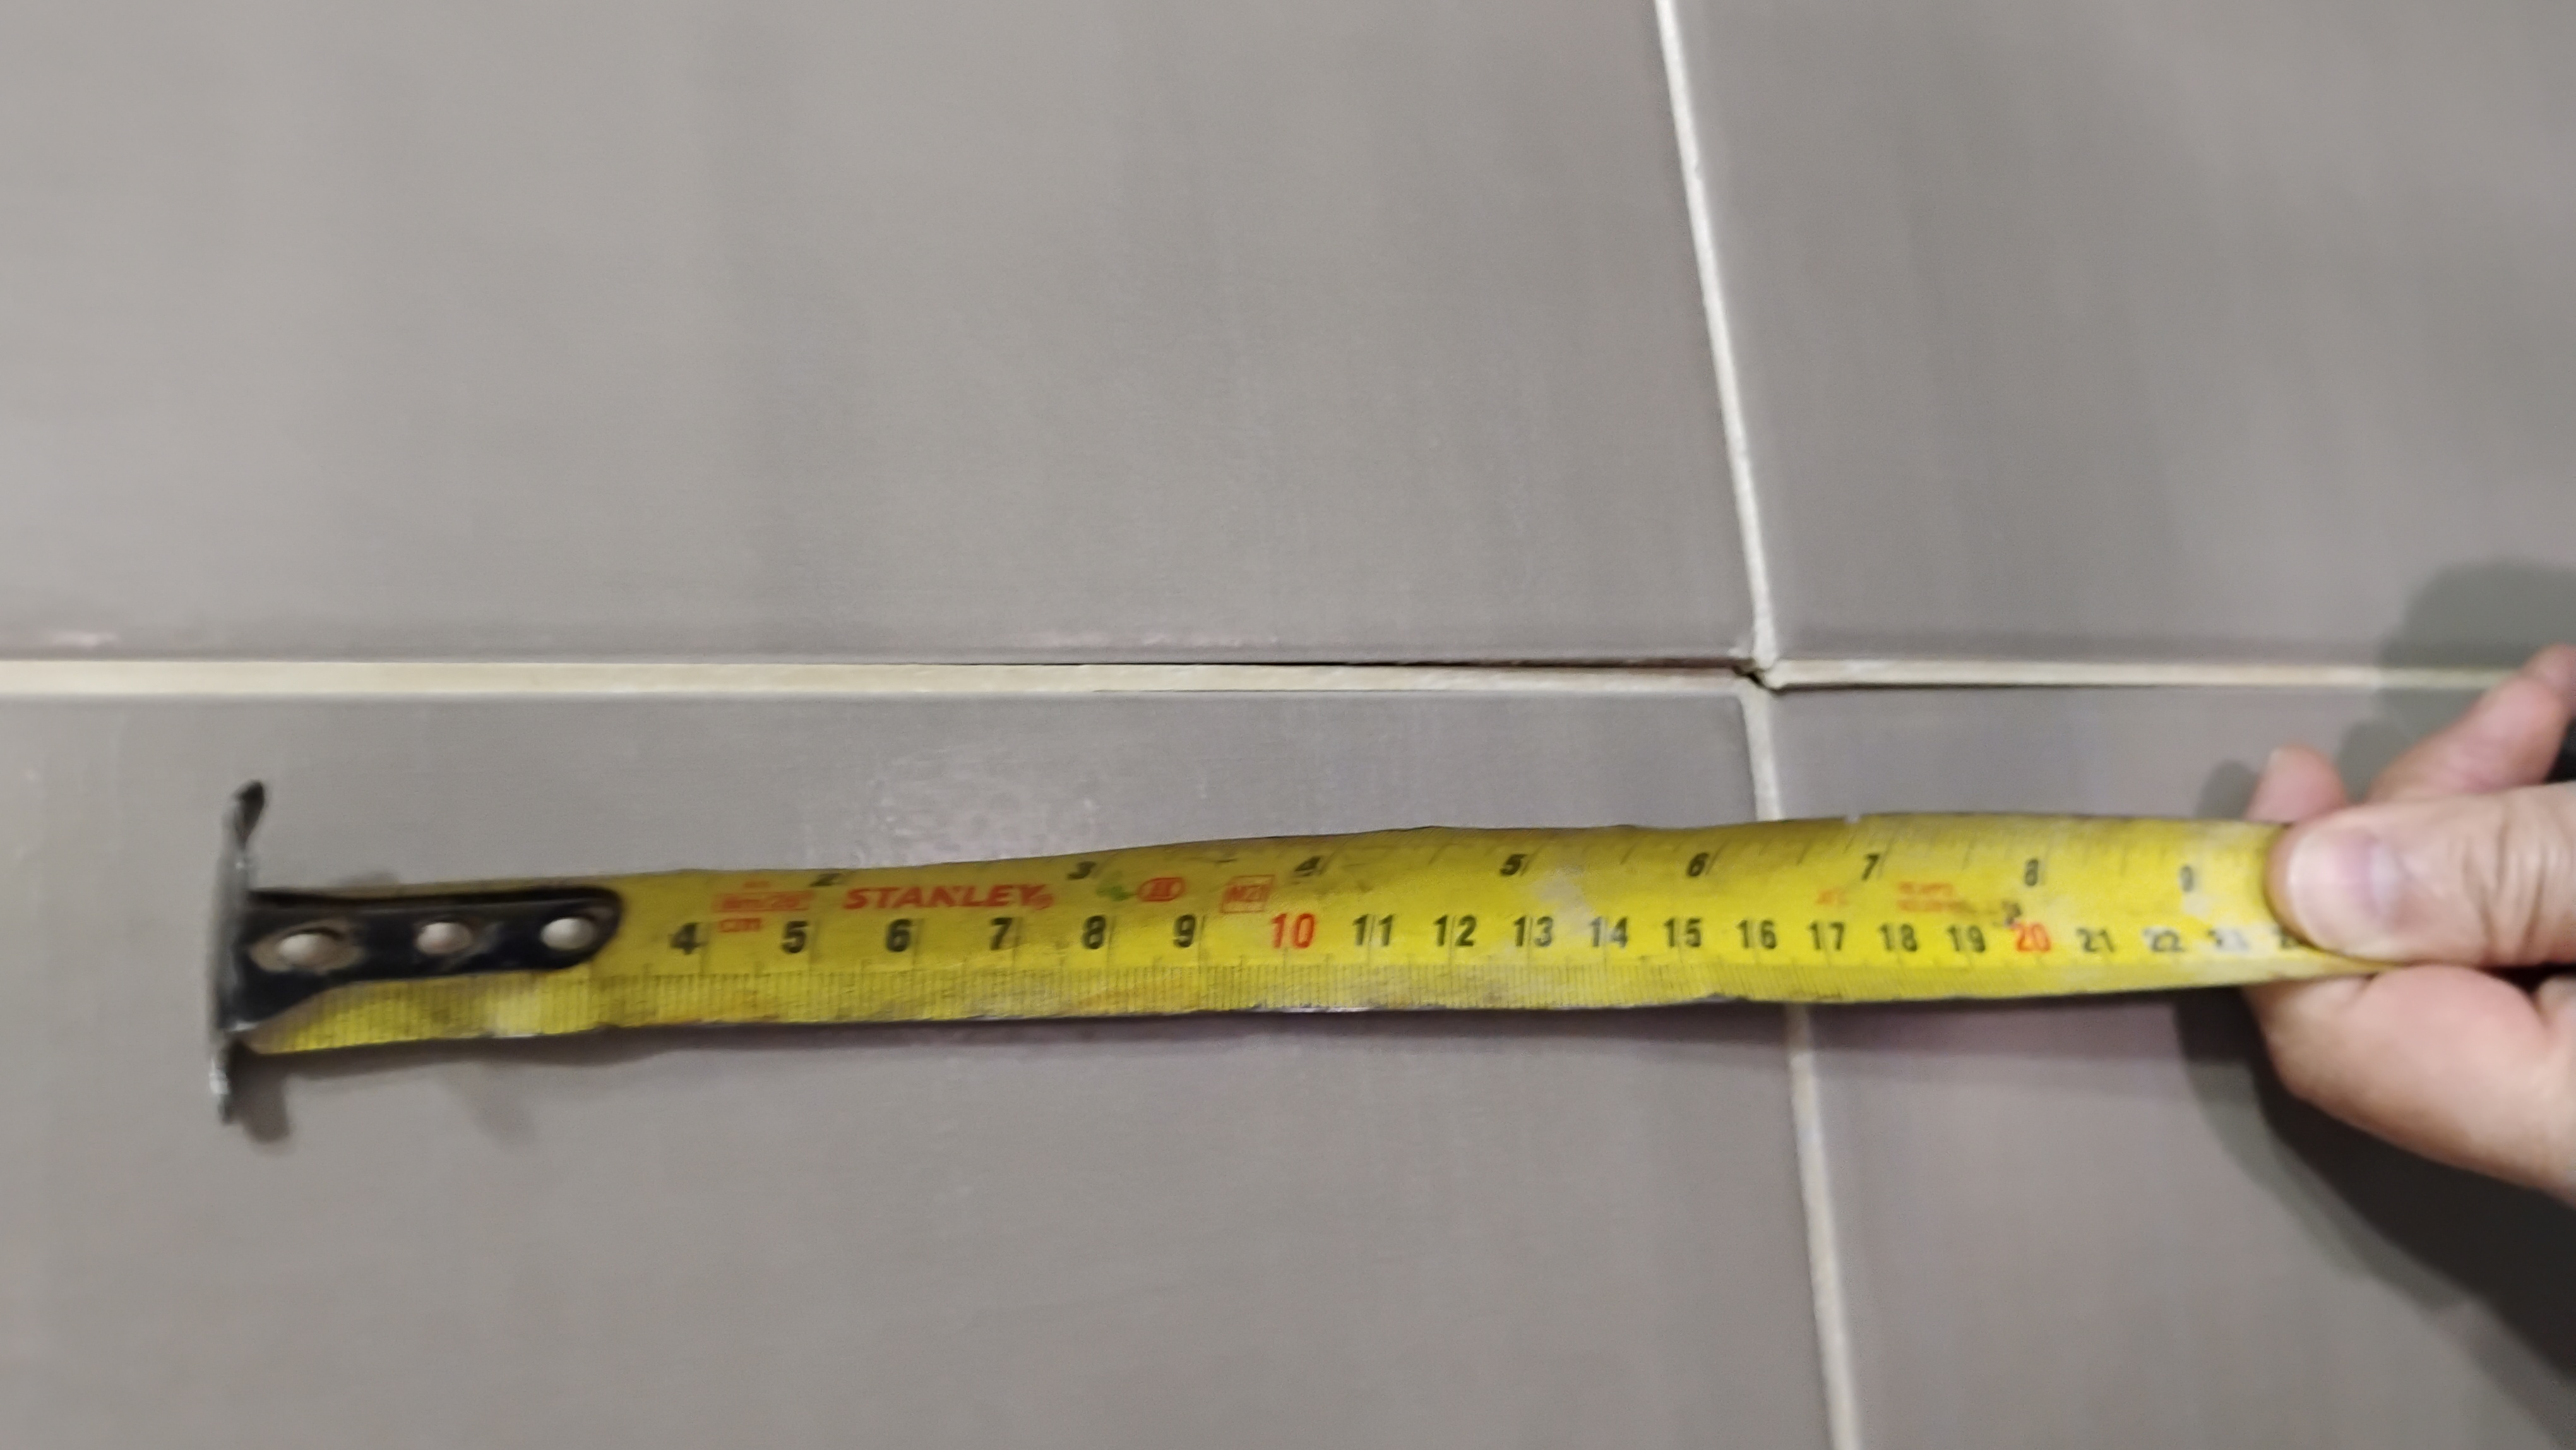
\includegraphics[width=\linewidth]{../img/IMG_20251109_151048194.jpg}\\[2pt]{\footnotesize\color{primary!60!black}Foto~42 -- 15:10:48}} \\[4pt]
\end{tabular}
\caption{Muro Oriental — Fisura por Concentración de Esfuerzos: Fotos 37 al 42.}\end{figure}
\newpage
\begin{figure}[H]
\centering
\begin{tabular}{cc}
\parbox{0.45\textwidth}{\centering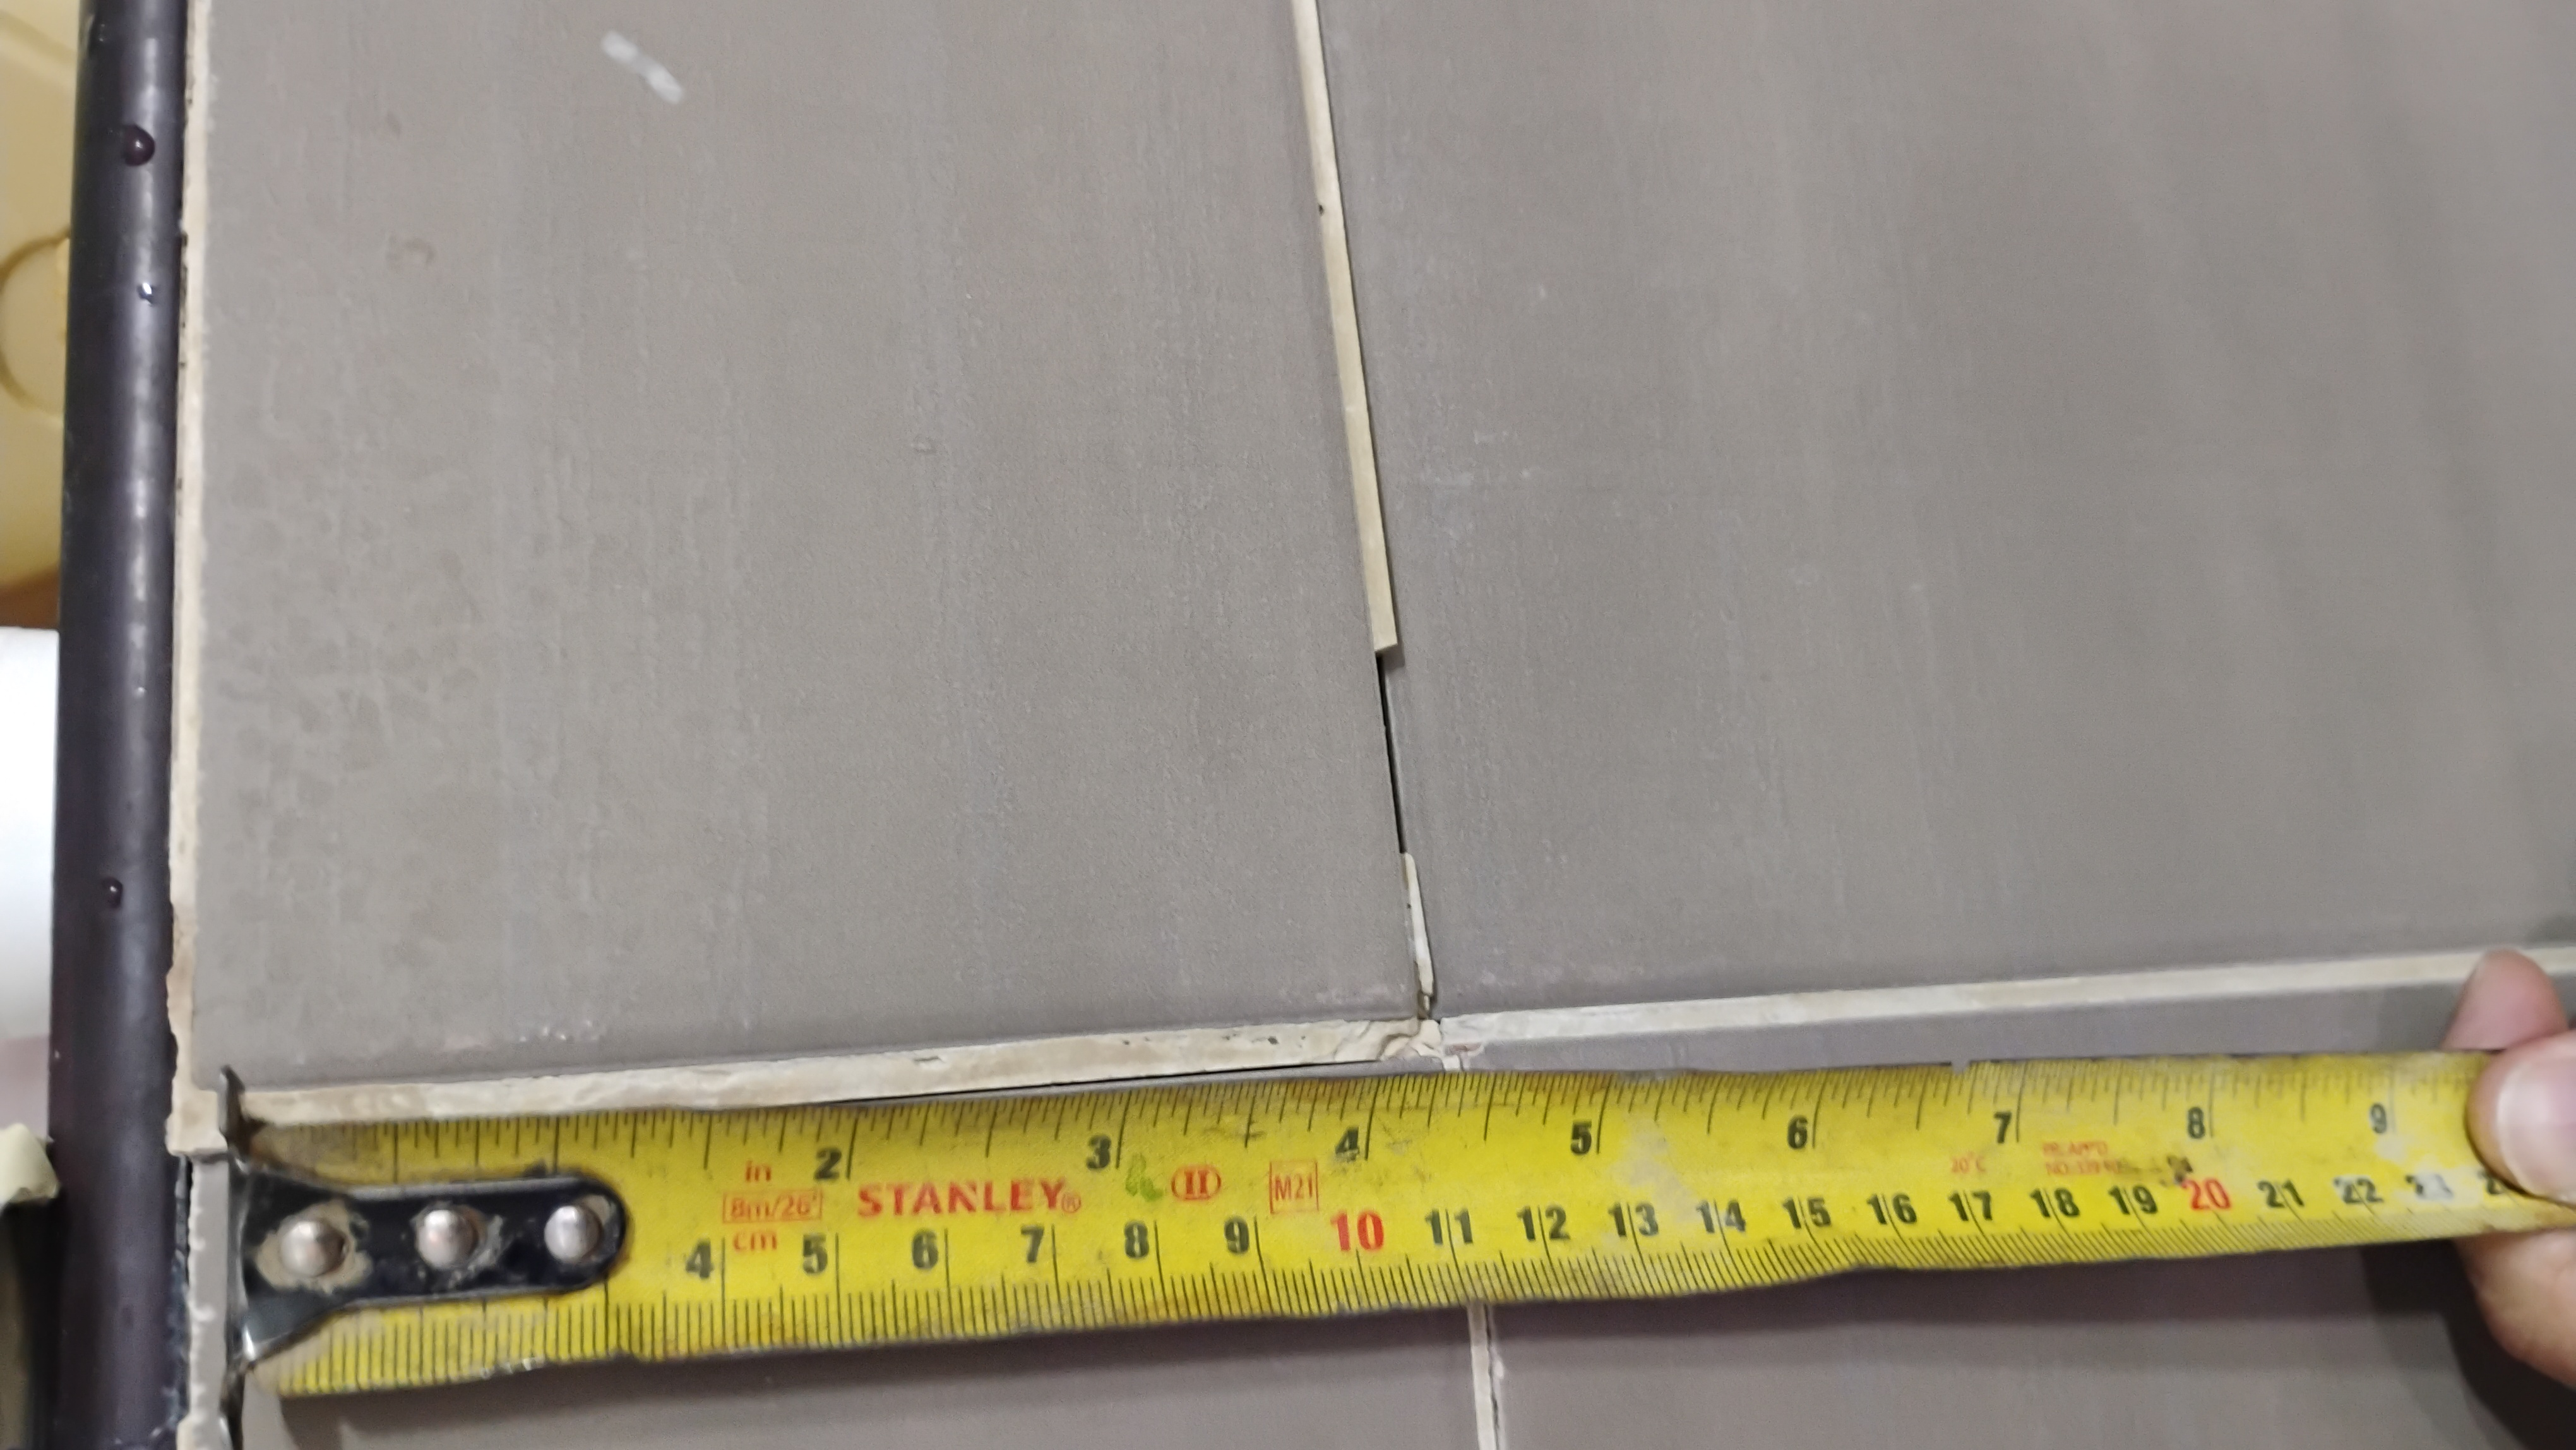
\includegraphics[width=\linewidth]{../img/IMG_20251109_151051793.jpg}\\[2pt]{\footnotesize\color{primary!60!black}Foto~43 -- 15:10:51}} & \parbox{0.45\textwidth}{\centering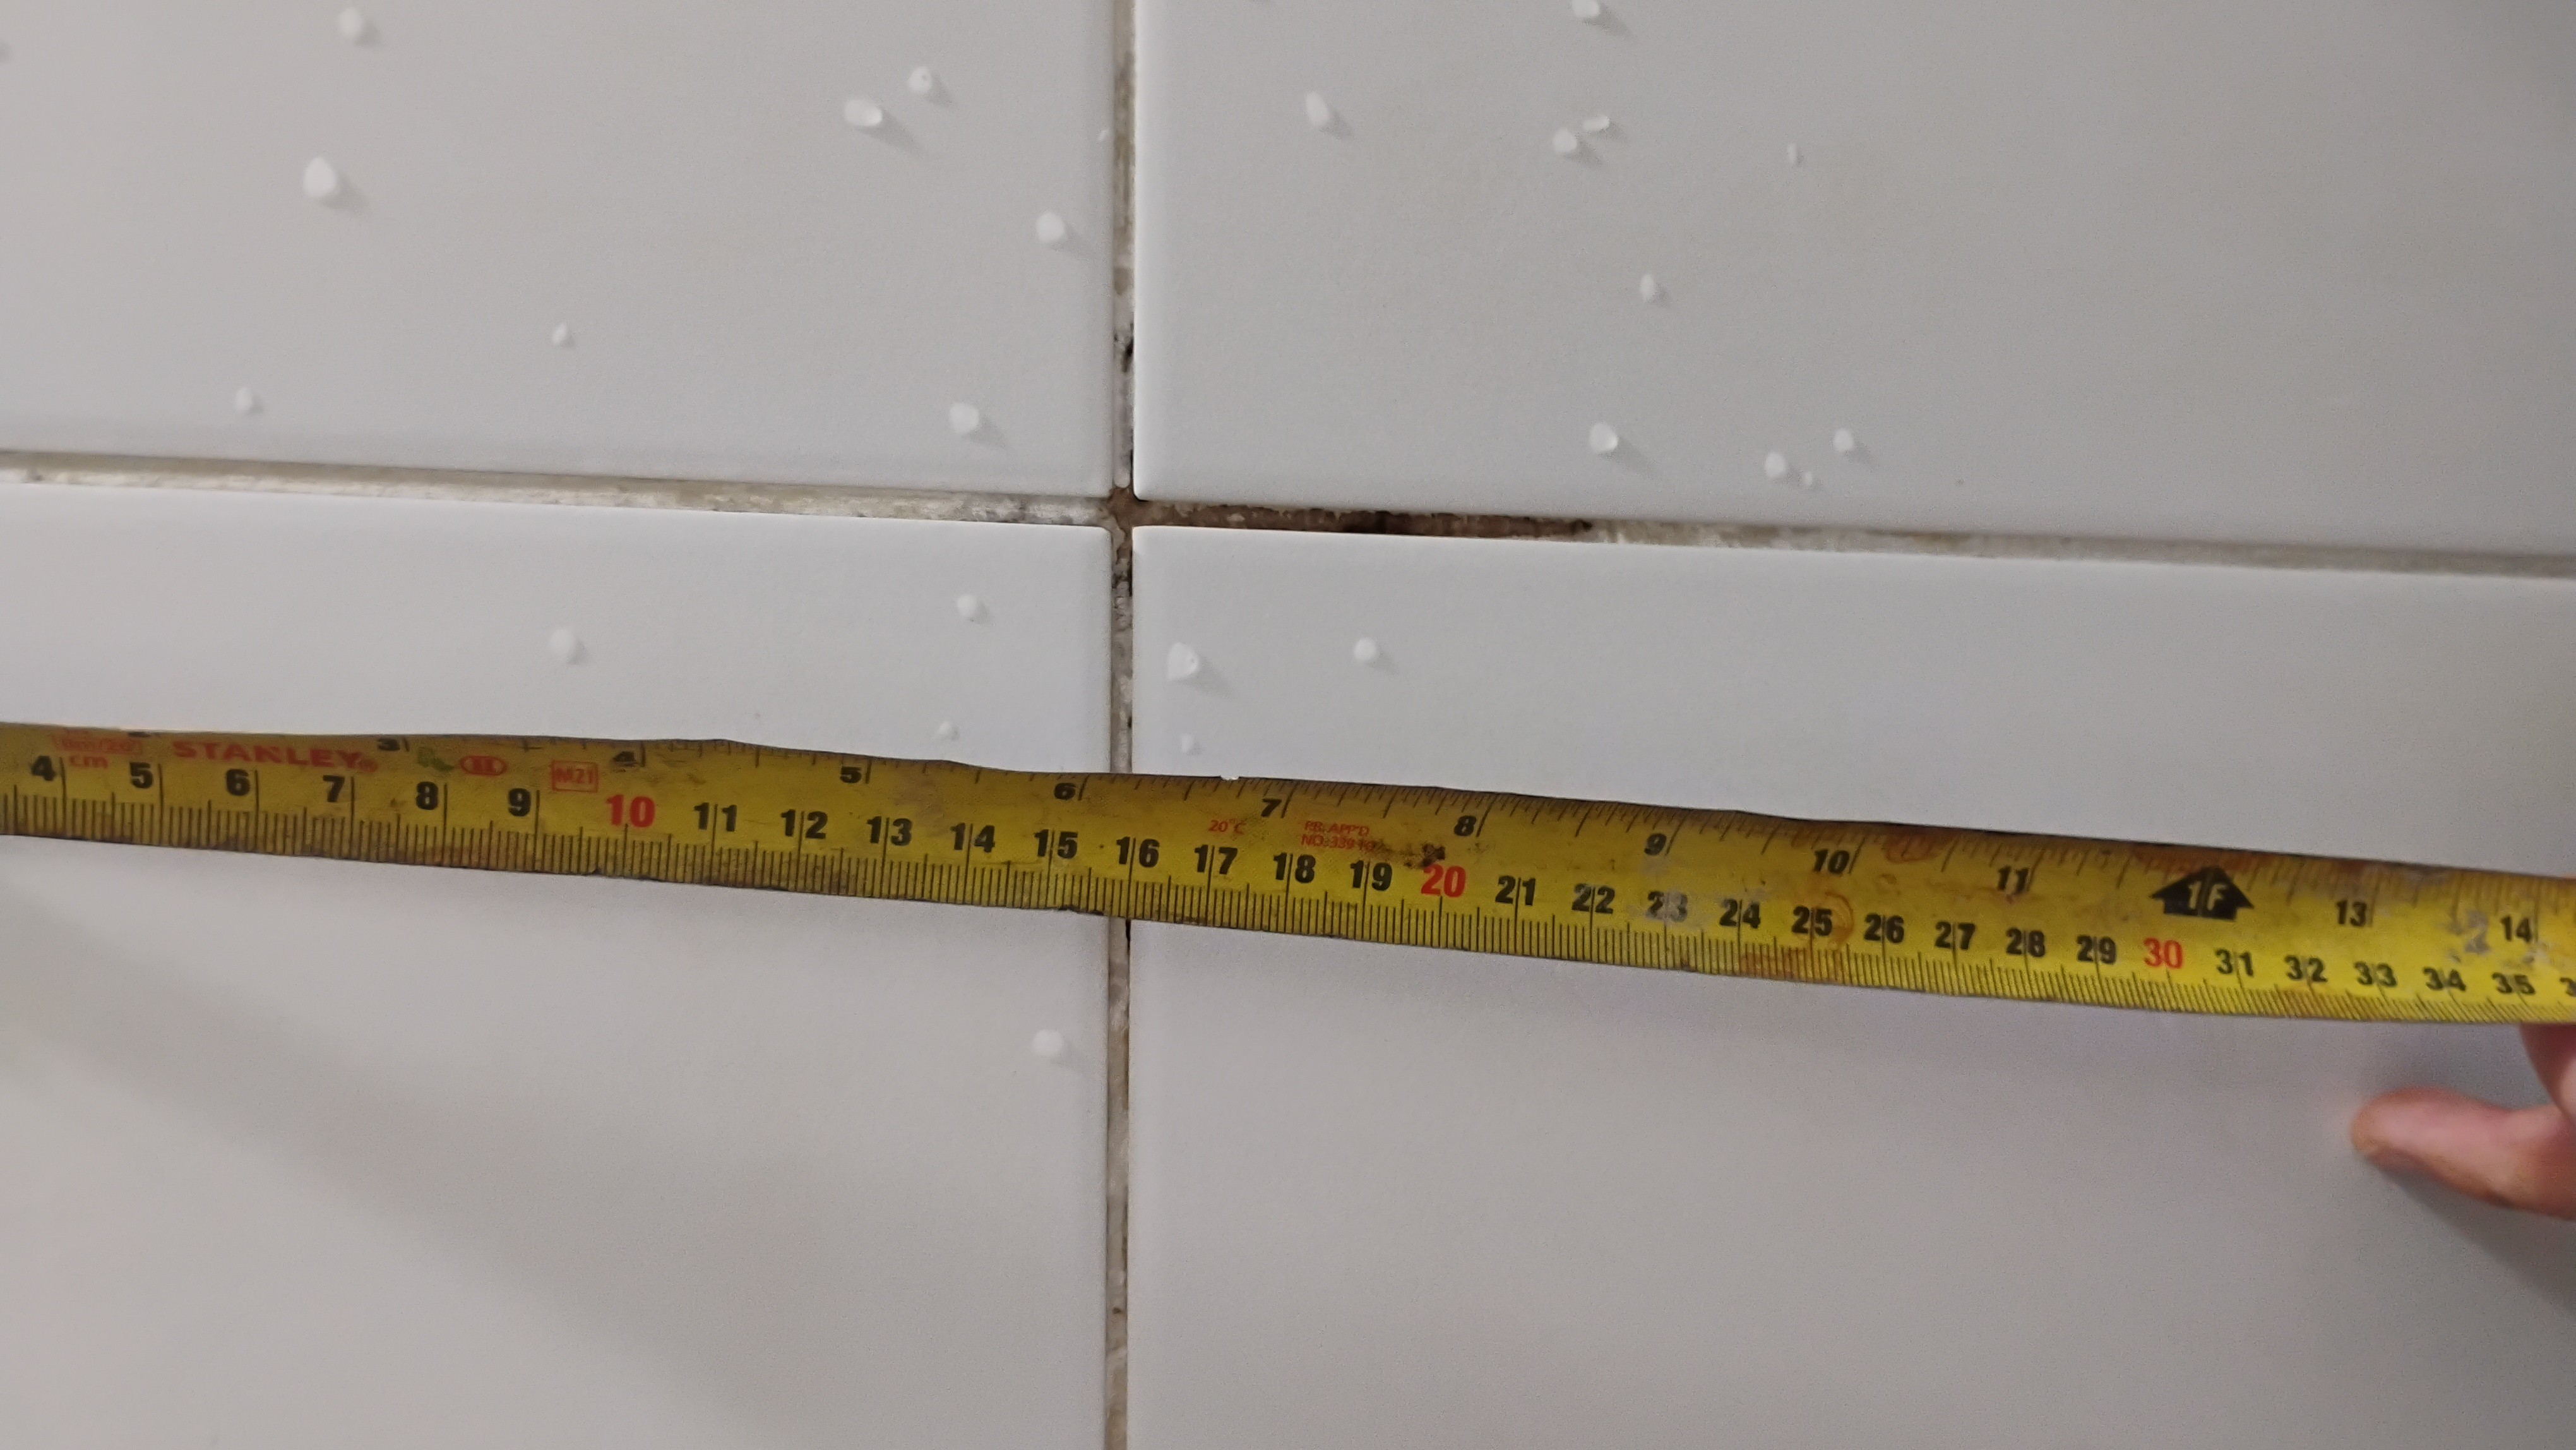
\includegraphics[width=\linewidth]{../img/IMG_20251109_151103248.jpg}\\[2pt]{\footnotesize\color{primary!60!black}Foto~44 -- 15:11:03}} \\[4pt]
\parbox{0.45\textwidth}{\centering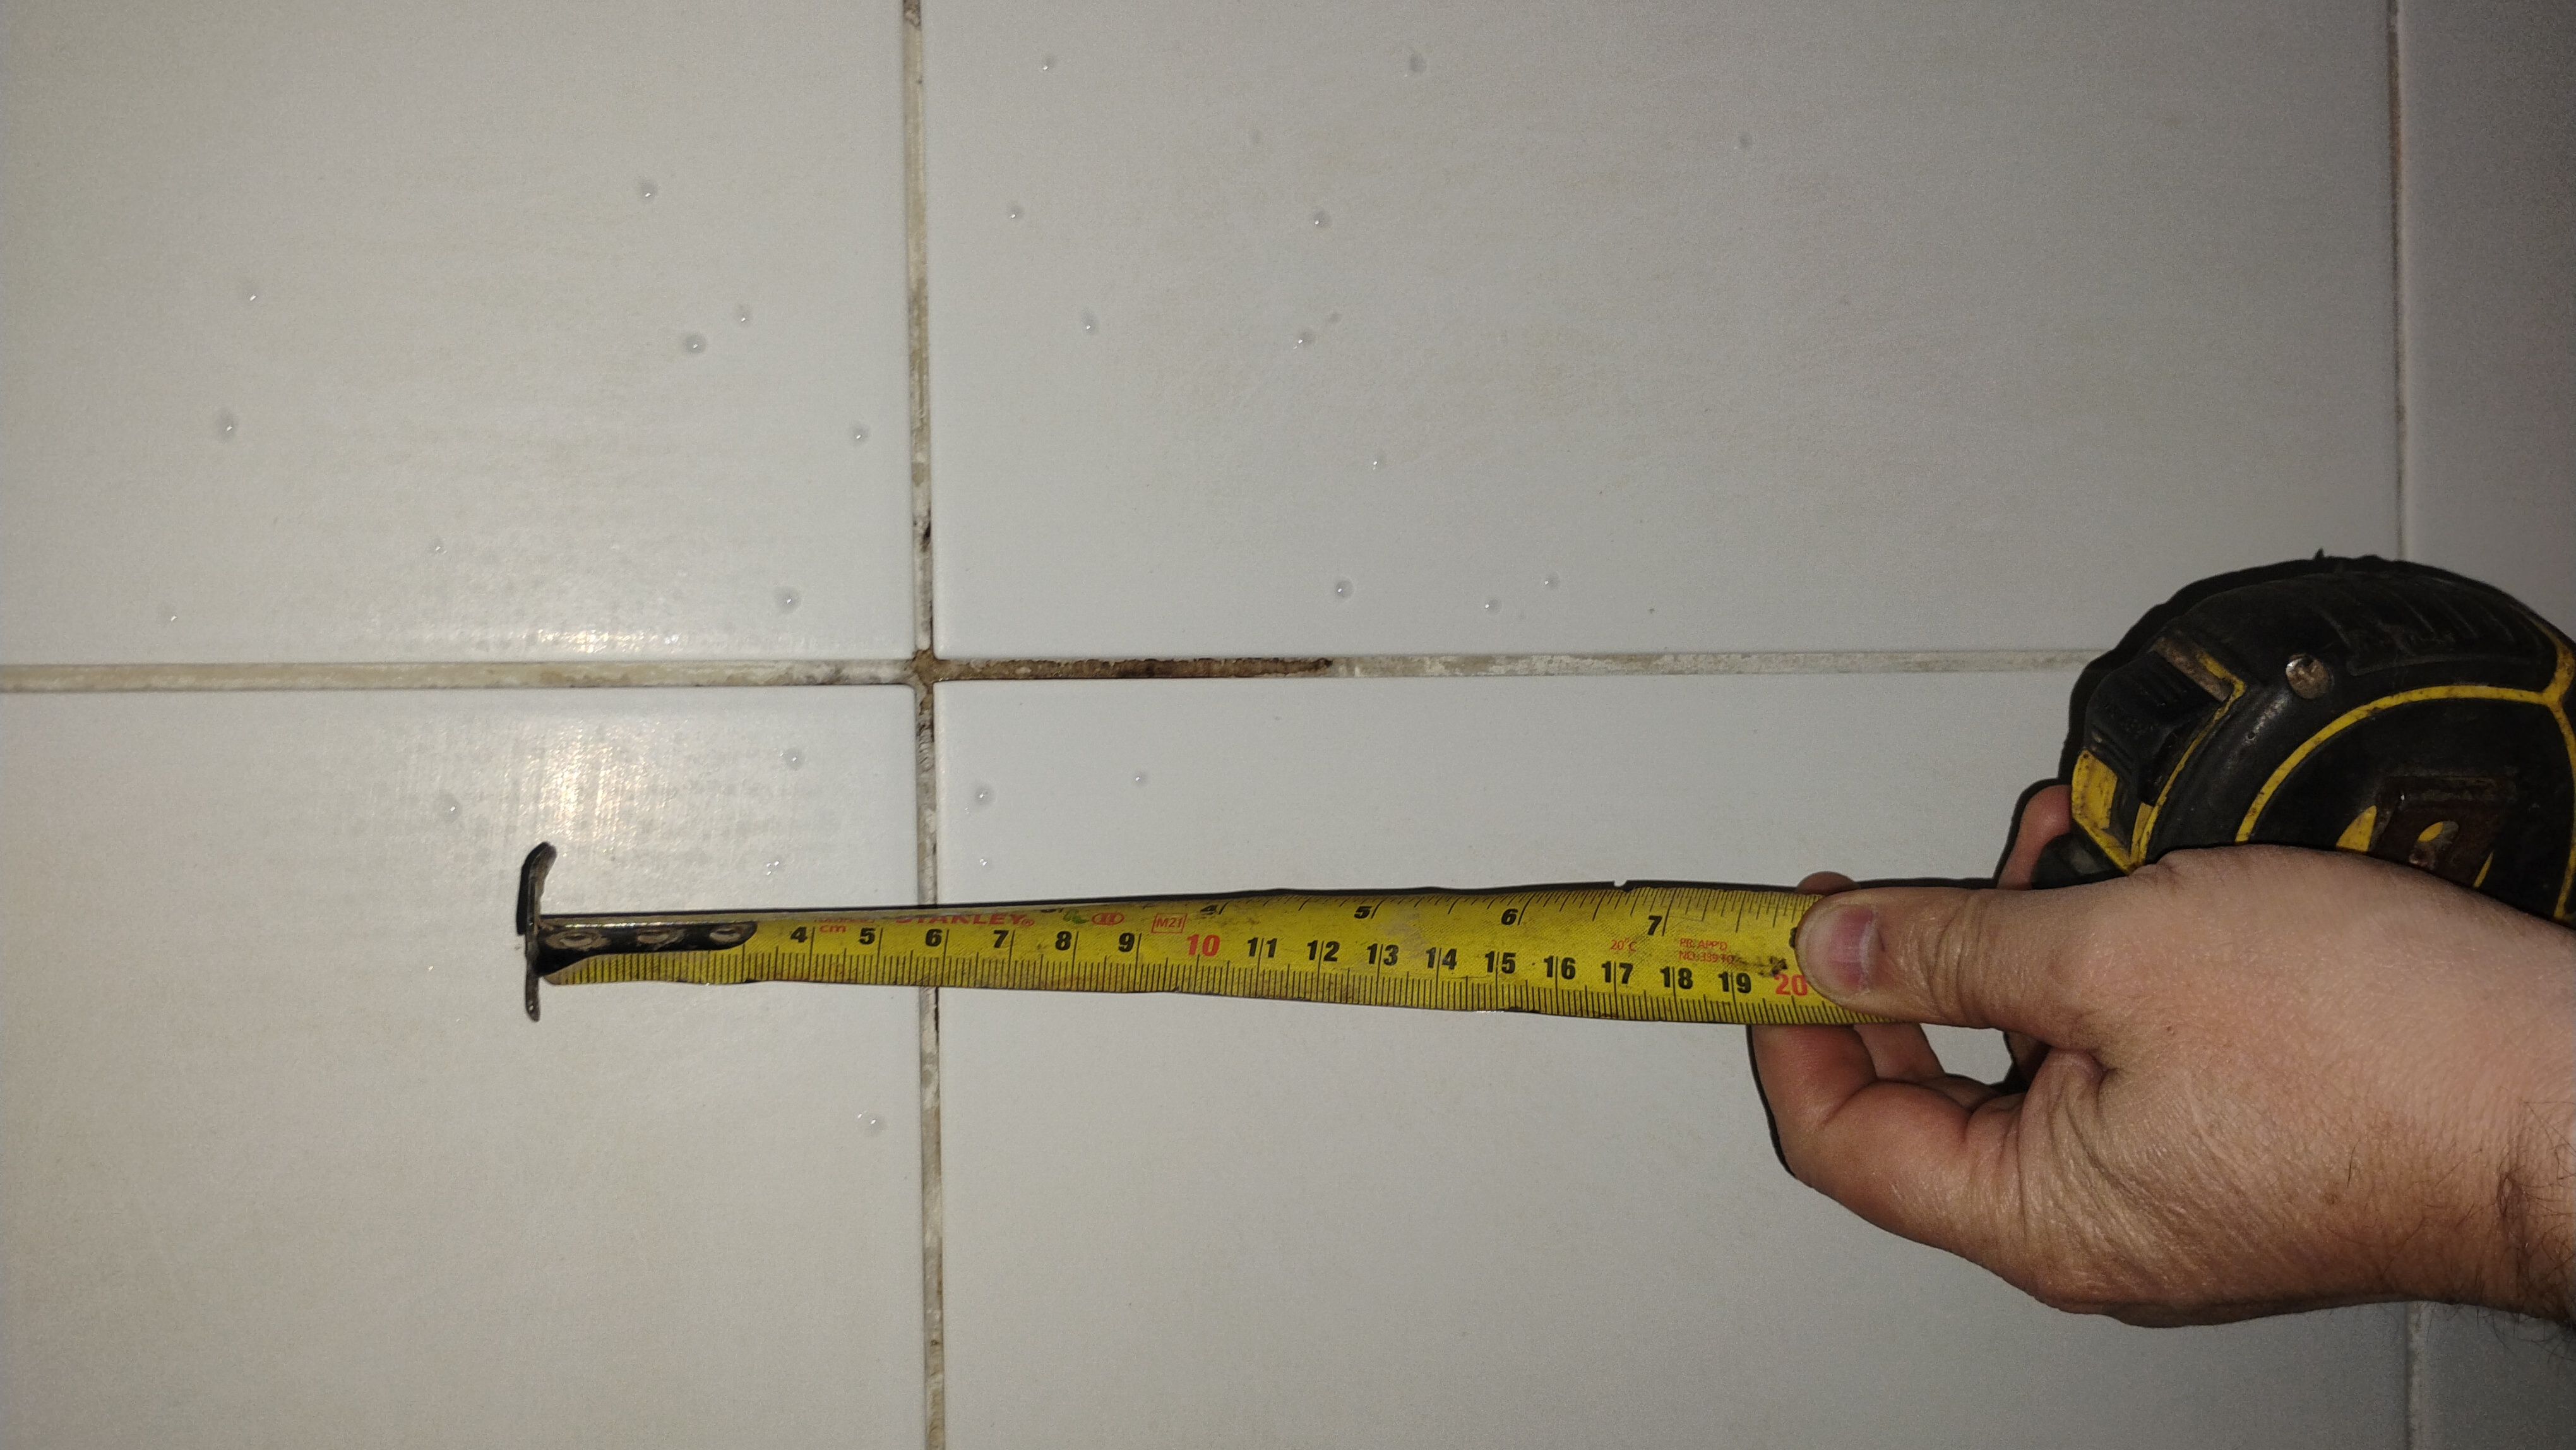
\includegraphics[width=\linewidth]{../img/IMG_20251109_151111424.jpg}\\[2pt]{\footnotesize\color{primary!60!black}Foto~45 -- 15:11:11}} & \parbox{0.45\textwidth}{\centering
\includegraphics[width=\linewidth]{../img/IMG_20251109_151329877.jpg}\\[2pt]{\footnotesize\color{primary!60!black}Foto~46 -- 15:13:29}} \\[4pt]
\parbox{0.45\textwidth}{\centering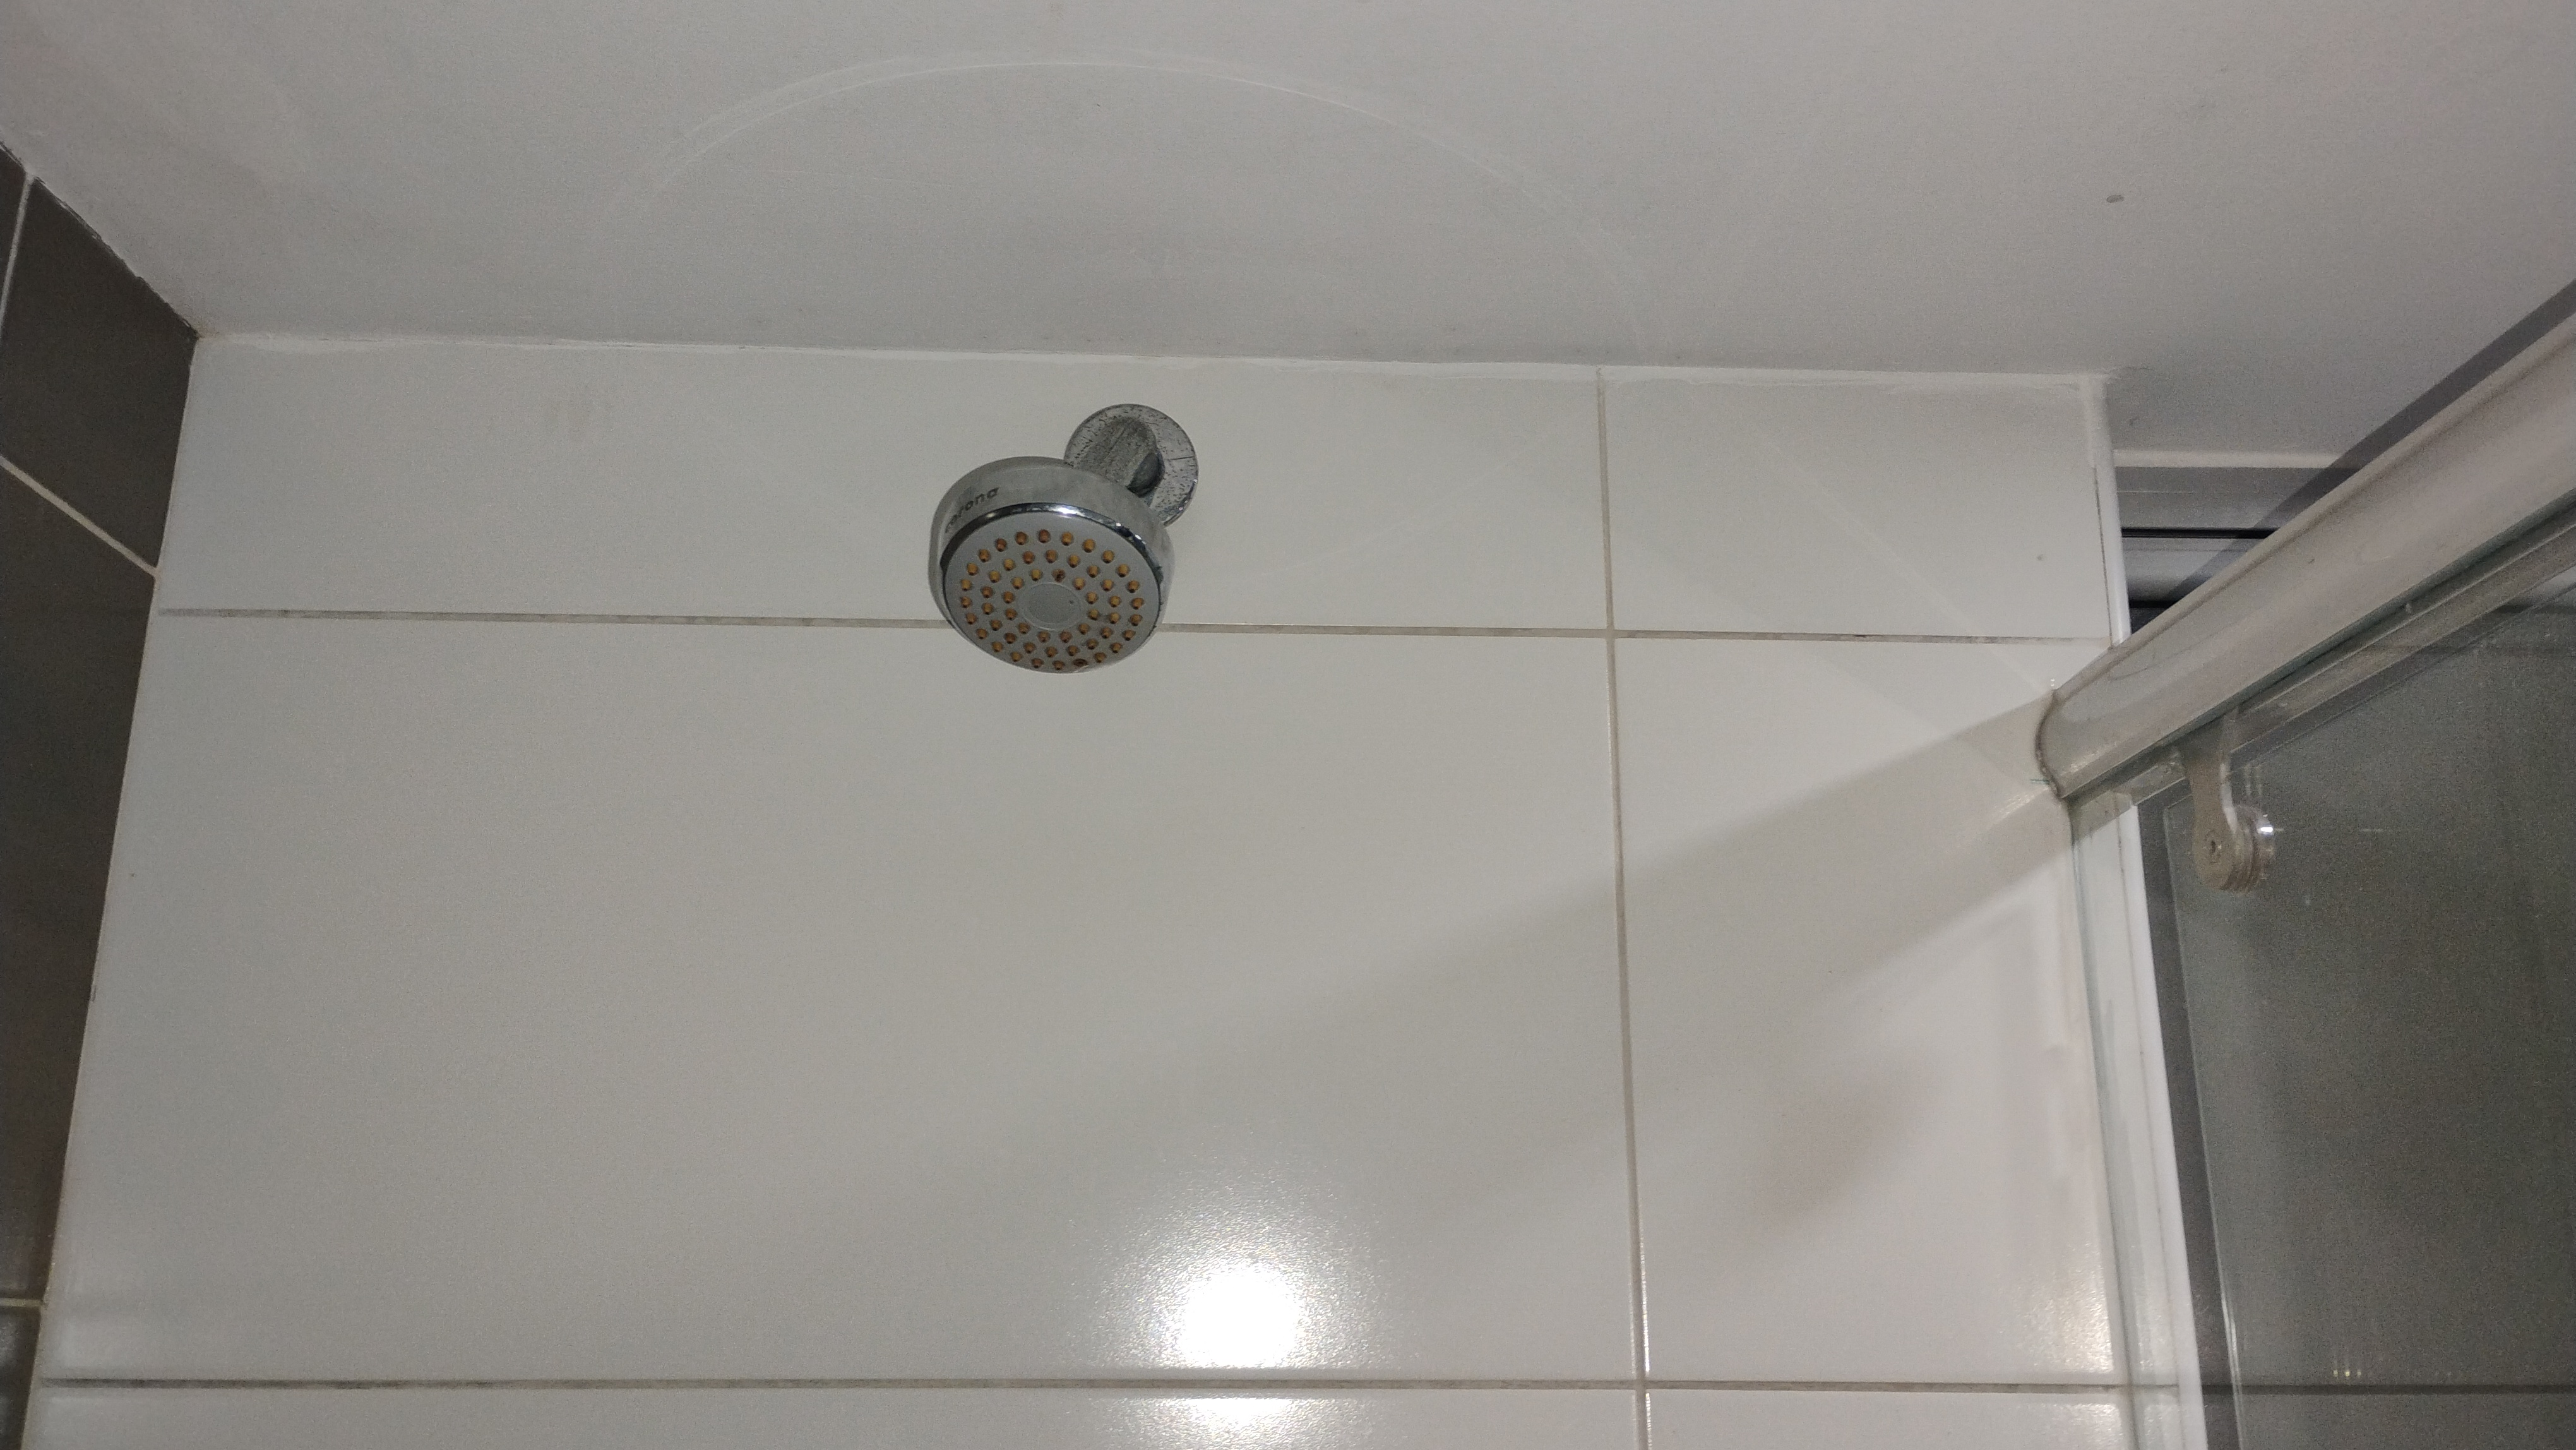
\includegraphics[width=\linewidth]{../img/IMG_20251109_151357220.jpg}\\[2pt]{\footnotesize\color{primary!60!black}Foto~47 -- 15:13:57}} & \parbox{0.45\textwidth}{\centering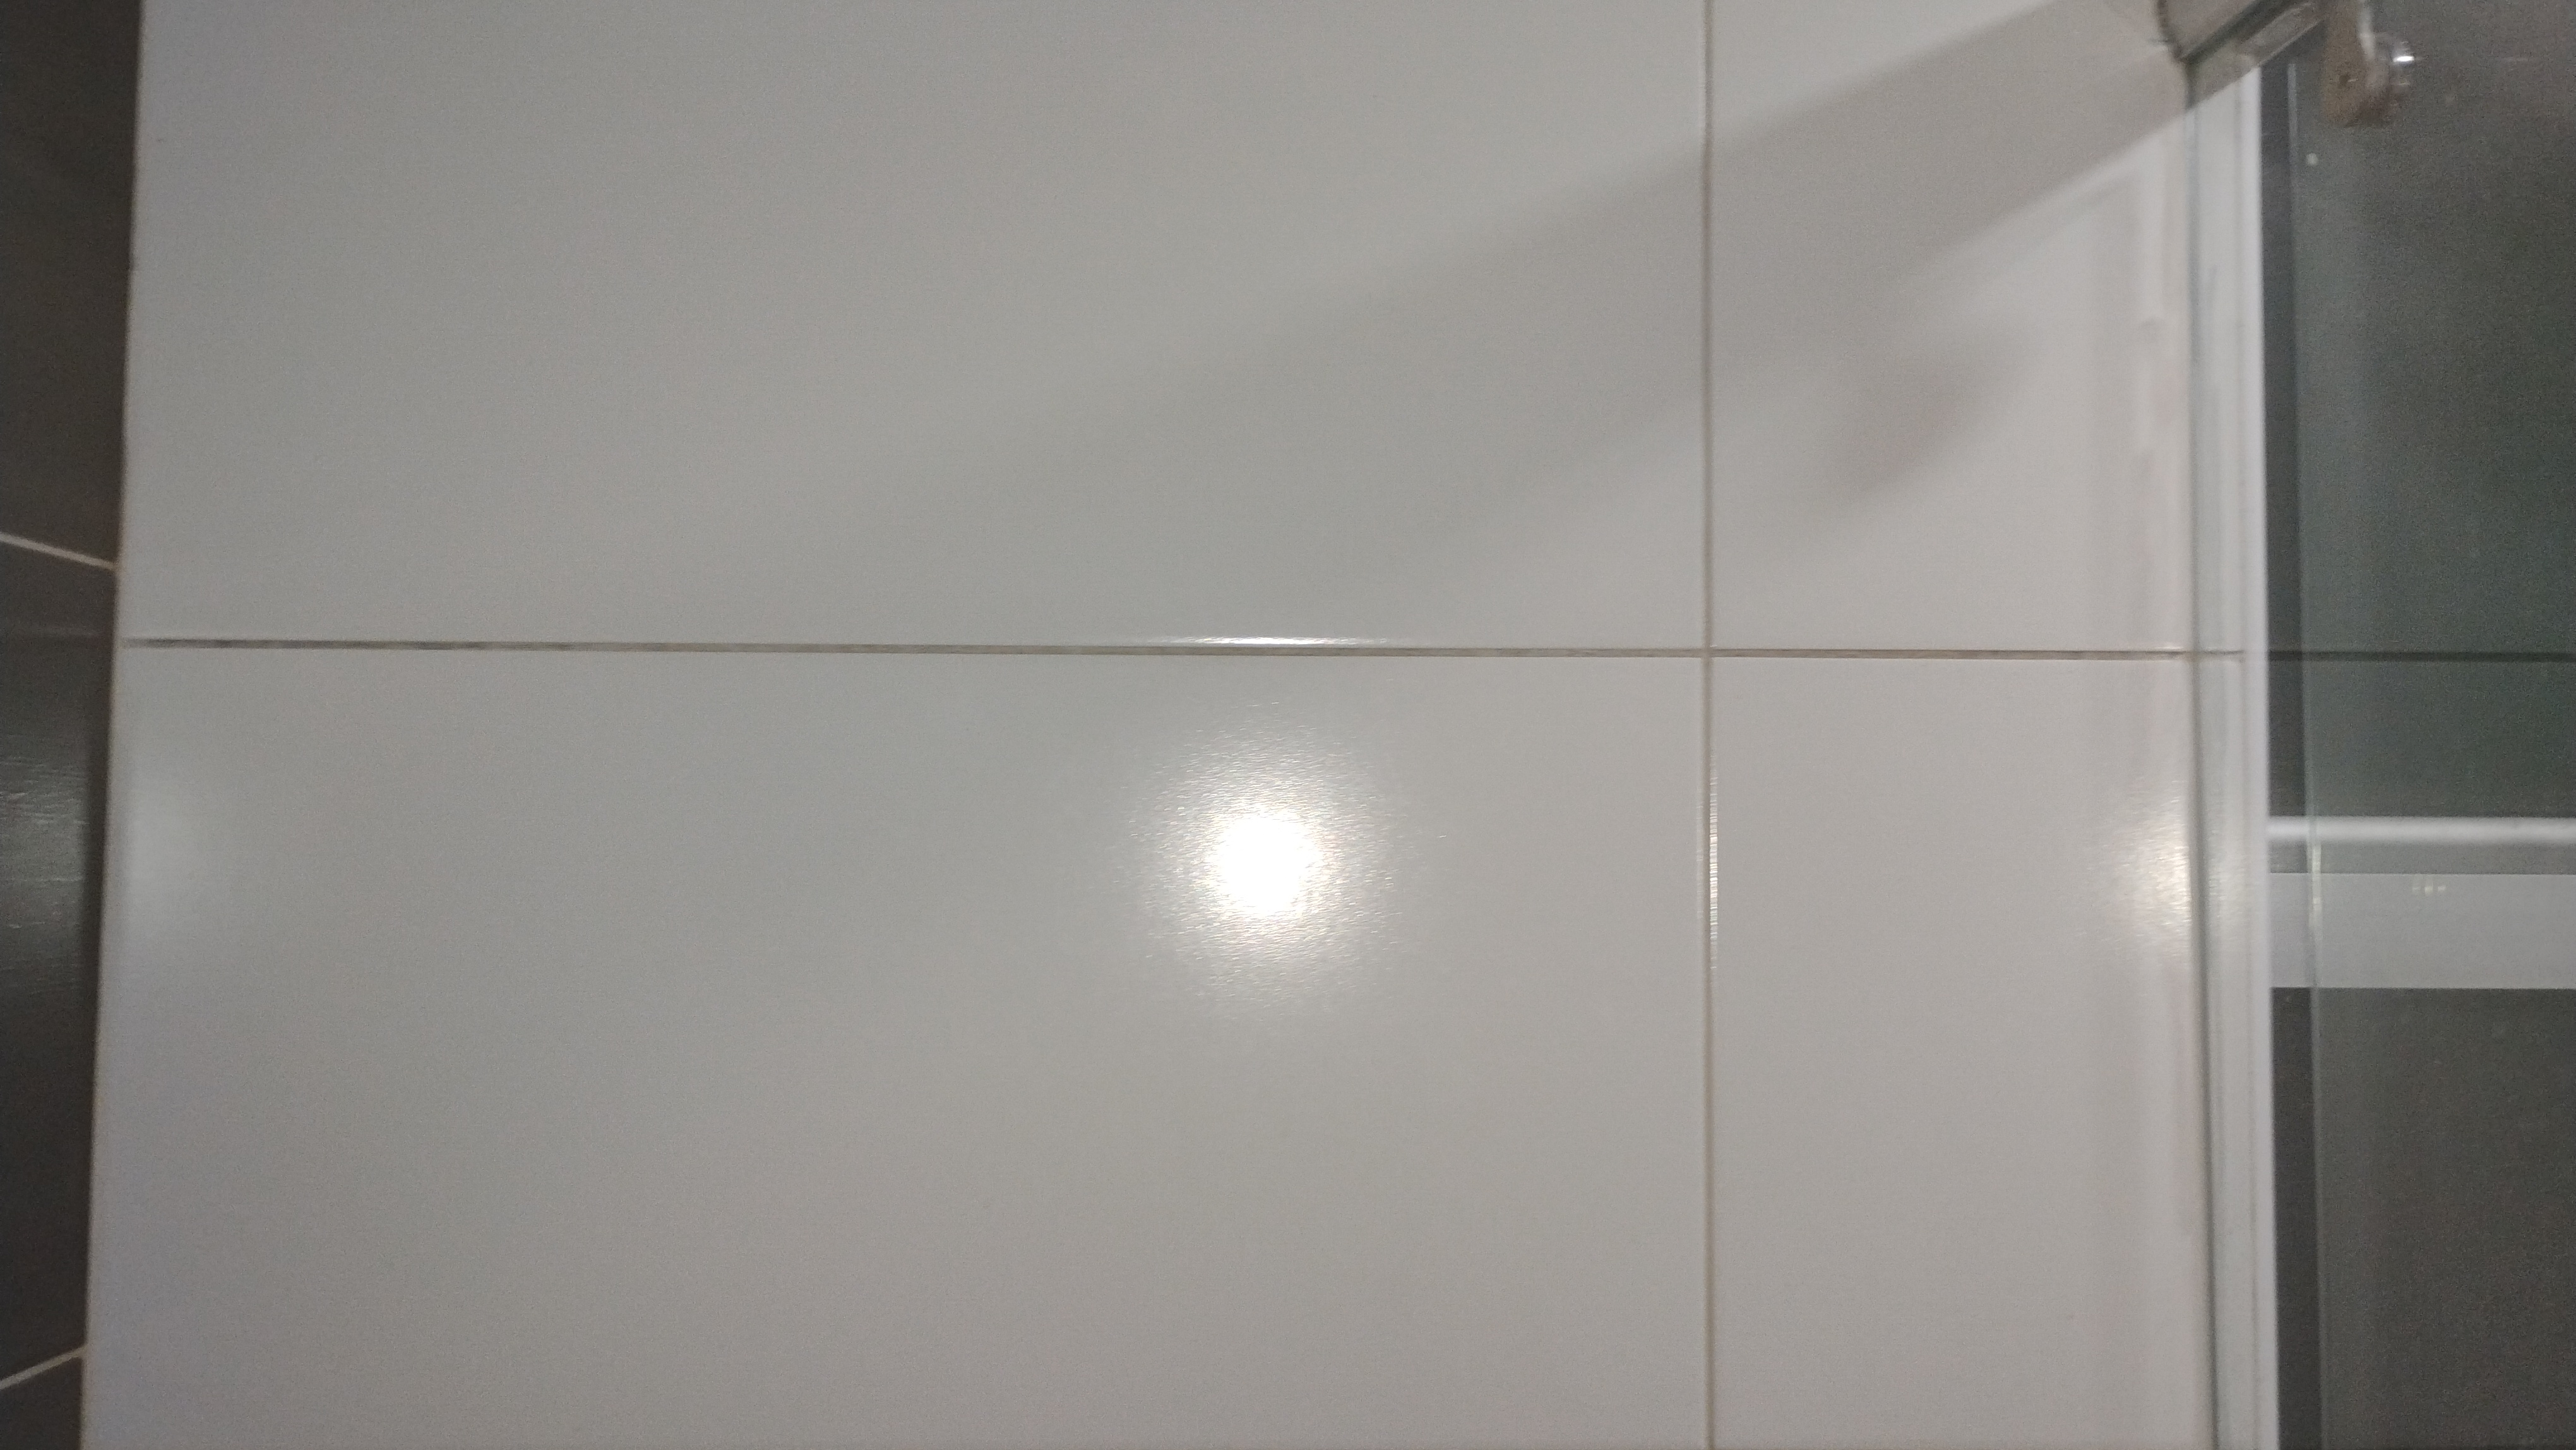
\includegraphics[width=\linewidth]{../img/IMG_20251109_151400914.jpg}\\[2pt]{\footnotesize\color{primary!60!black}Foto~48 -- 15:14:00}} \\[4pt]
\end{tabular}
\caption{Cielorraso — Humedad y Desprendimiento de Pañete: Fotos 43 al 48.}\end{figure}
\newpage
\begin{figure}[H]
\centering
\begin{tabular}{cc}
\parbox{0.45\textwidth}{\centering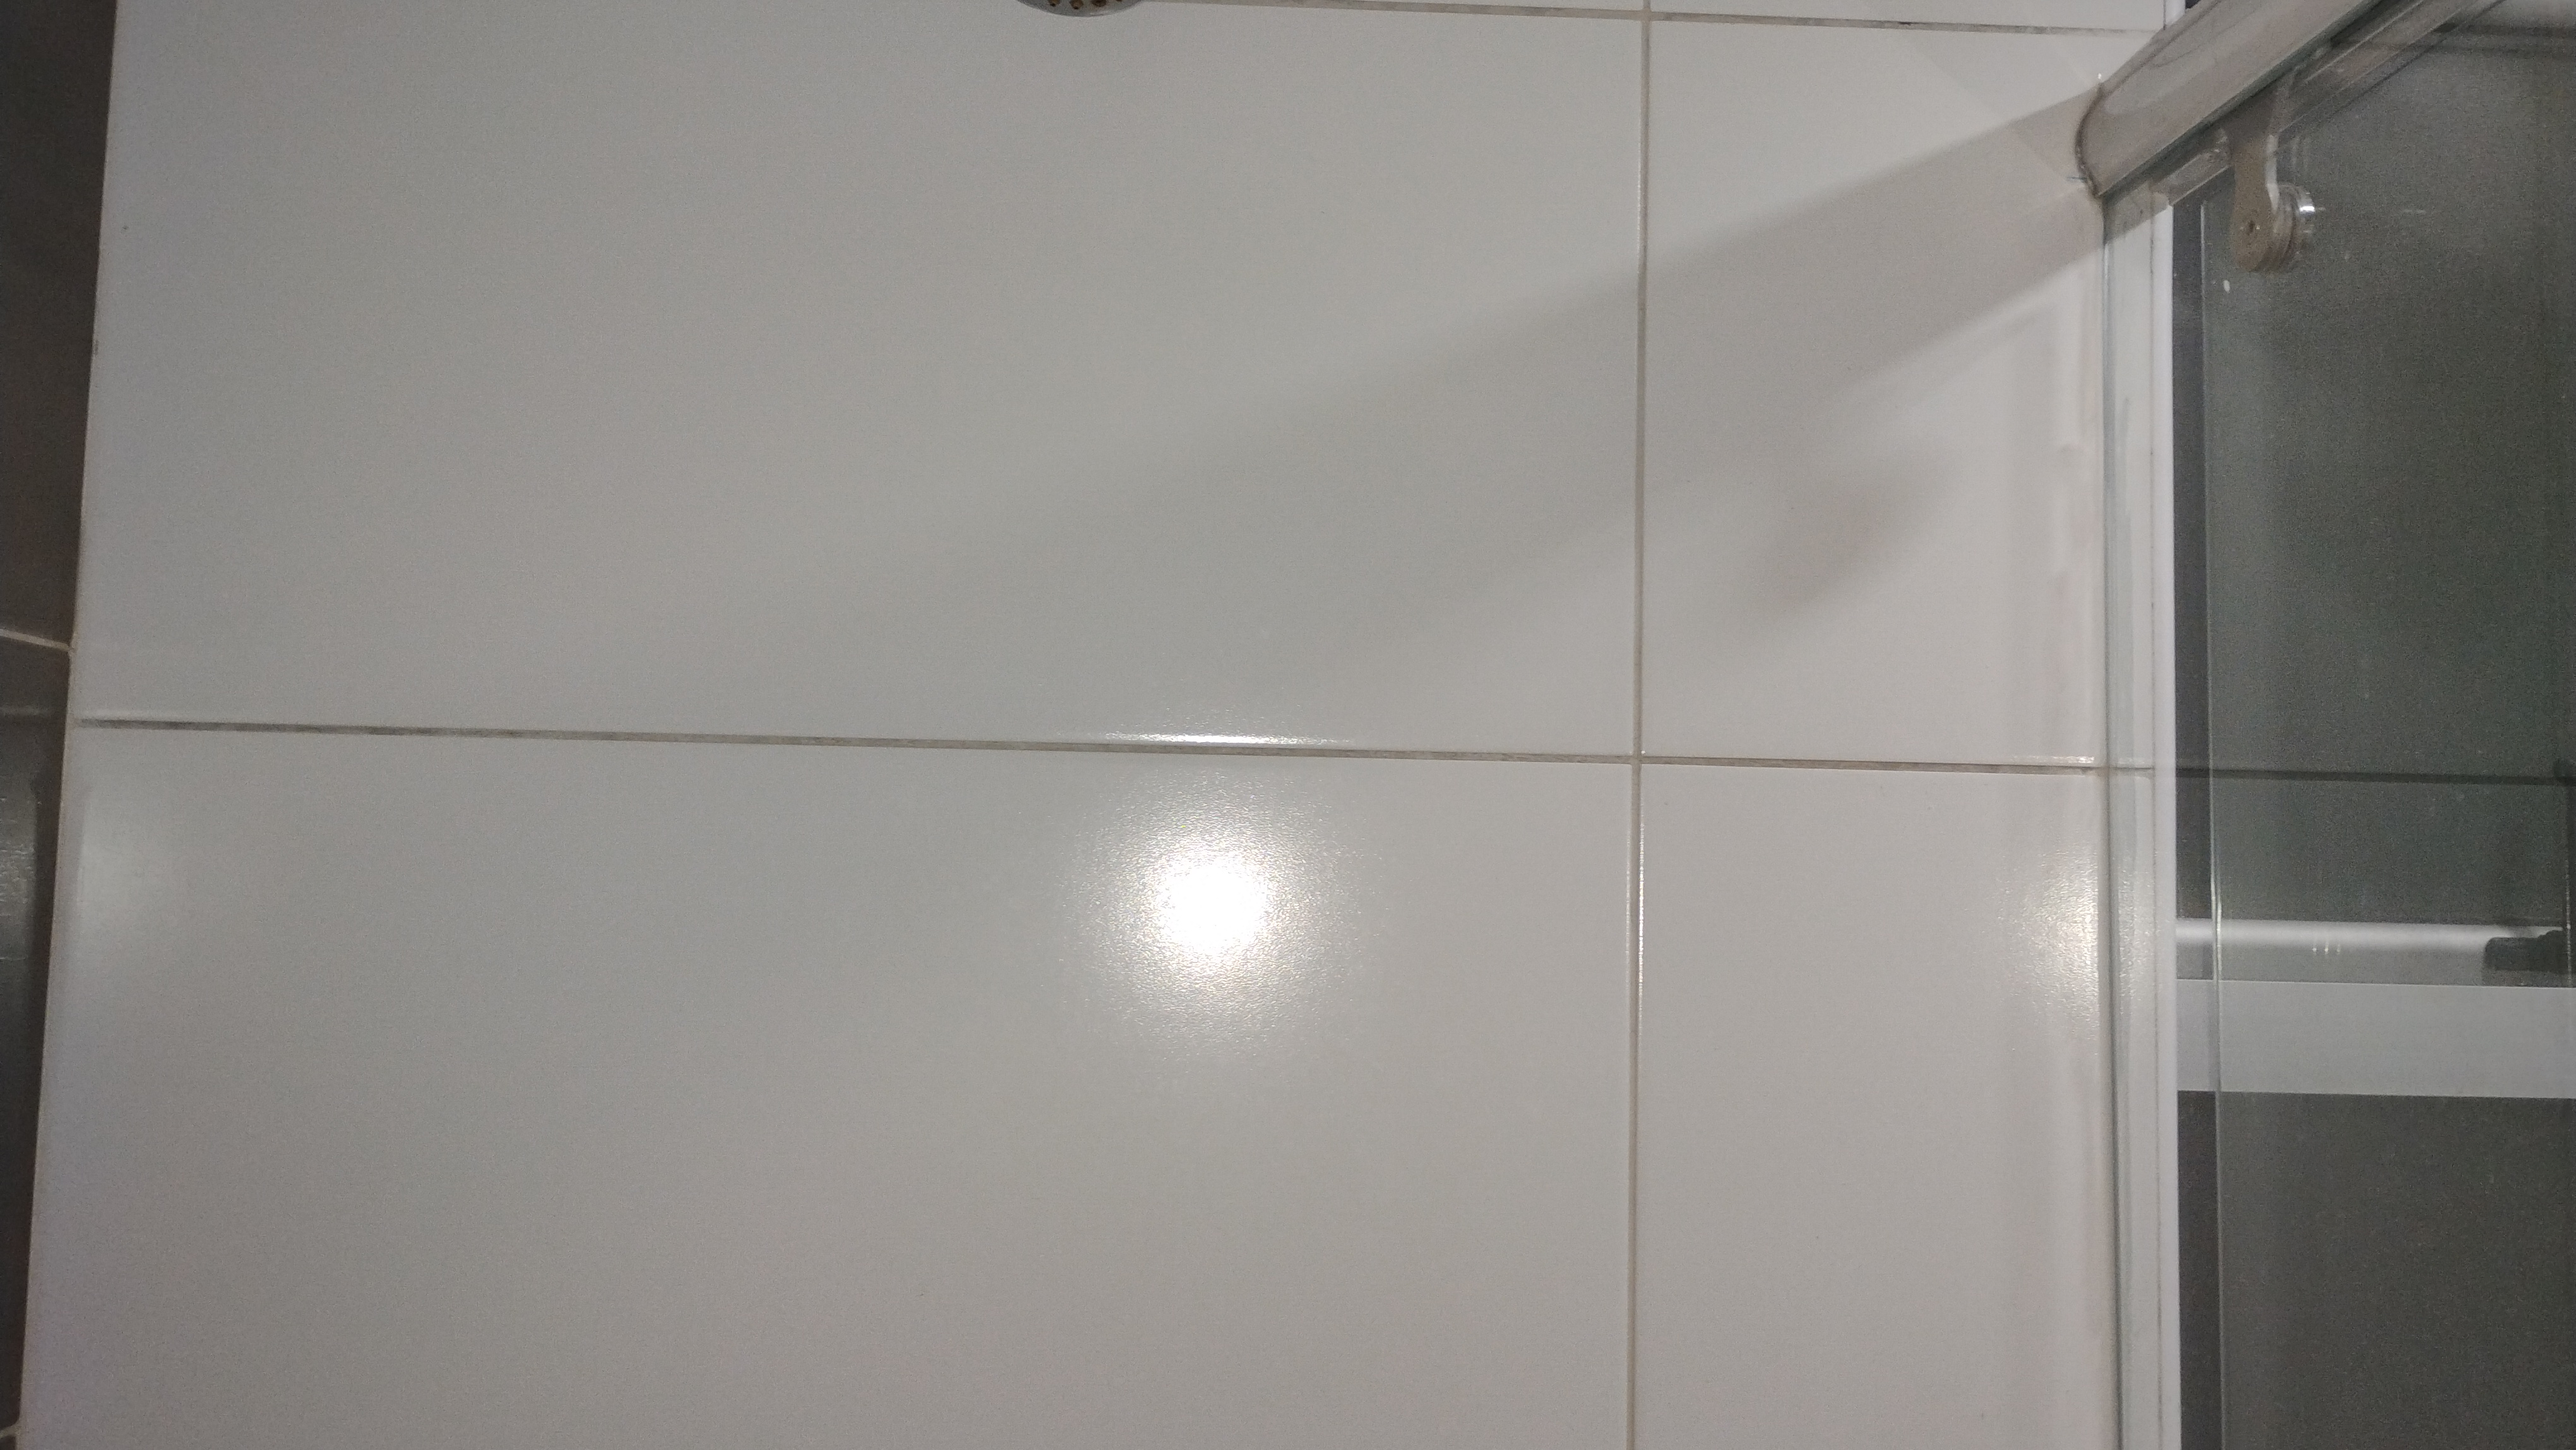
\includegraphics[width=\linewidth]{../img/IMG_20251109_151411256.jpg}\\[2pt]{\footnotesize\color{primary!60!black}Foto~49 -- 15:14:11}} & \parbox{0.45\textwidth}{\centering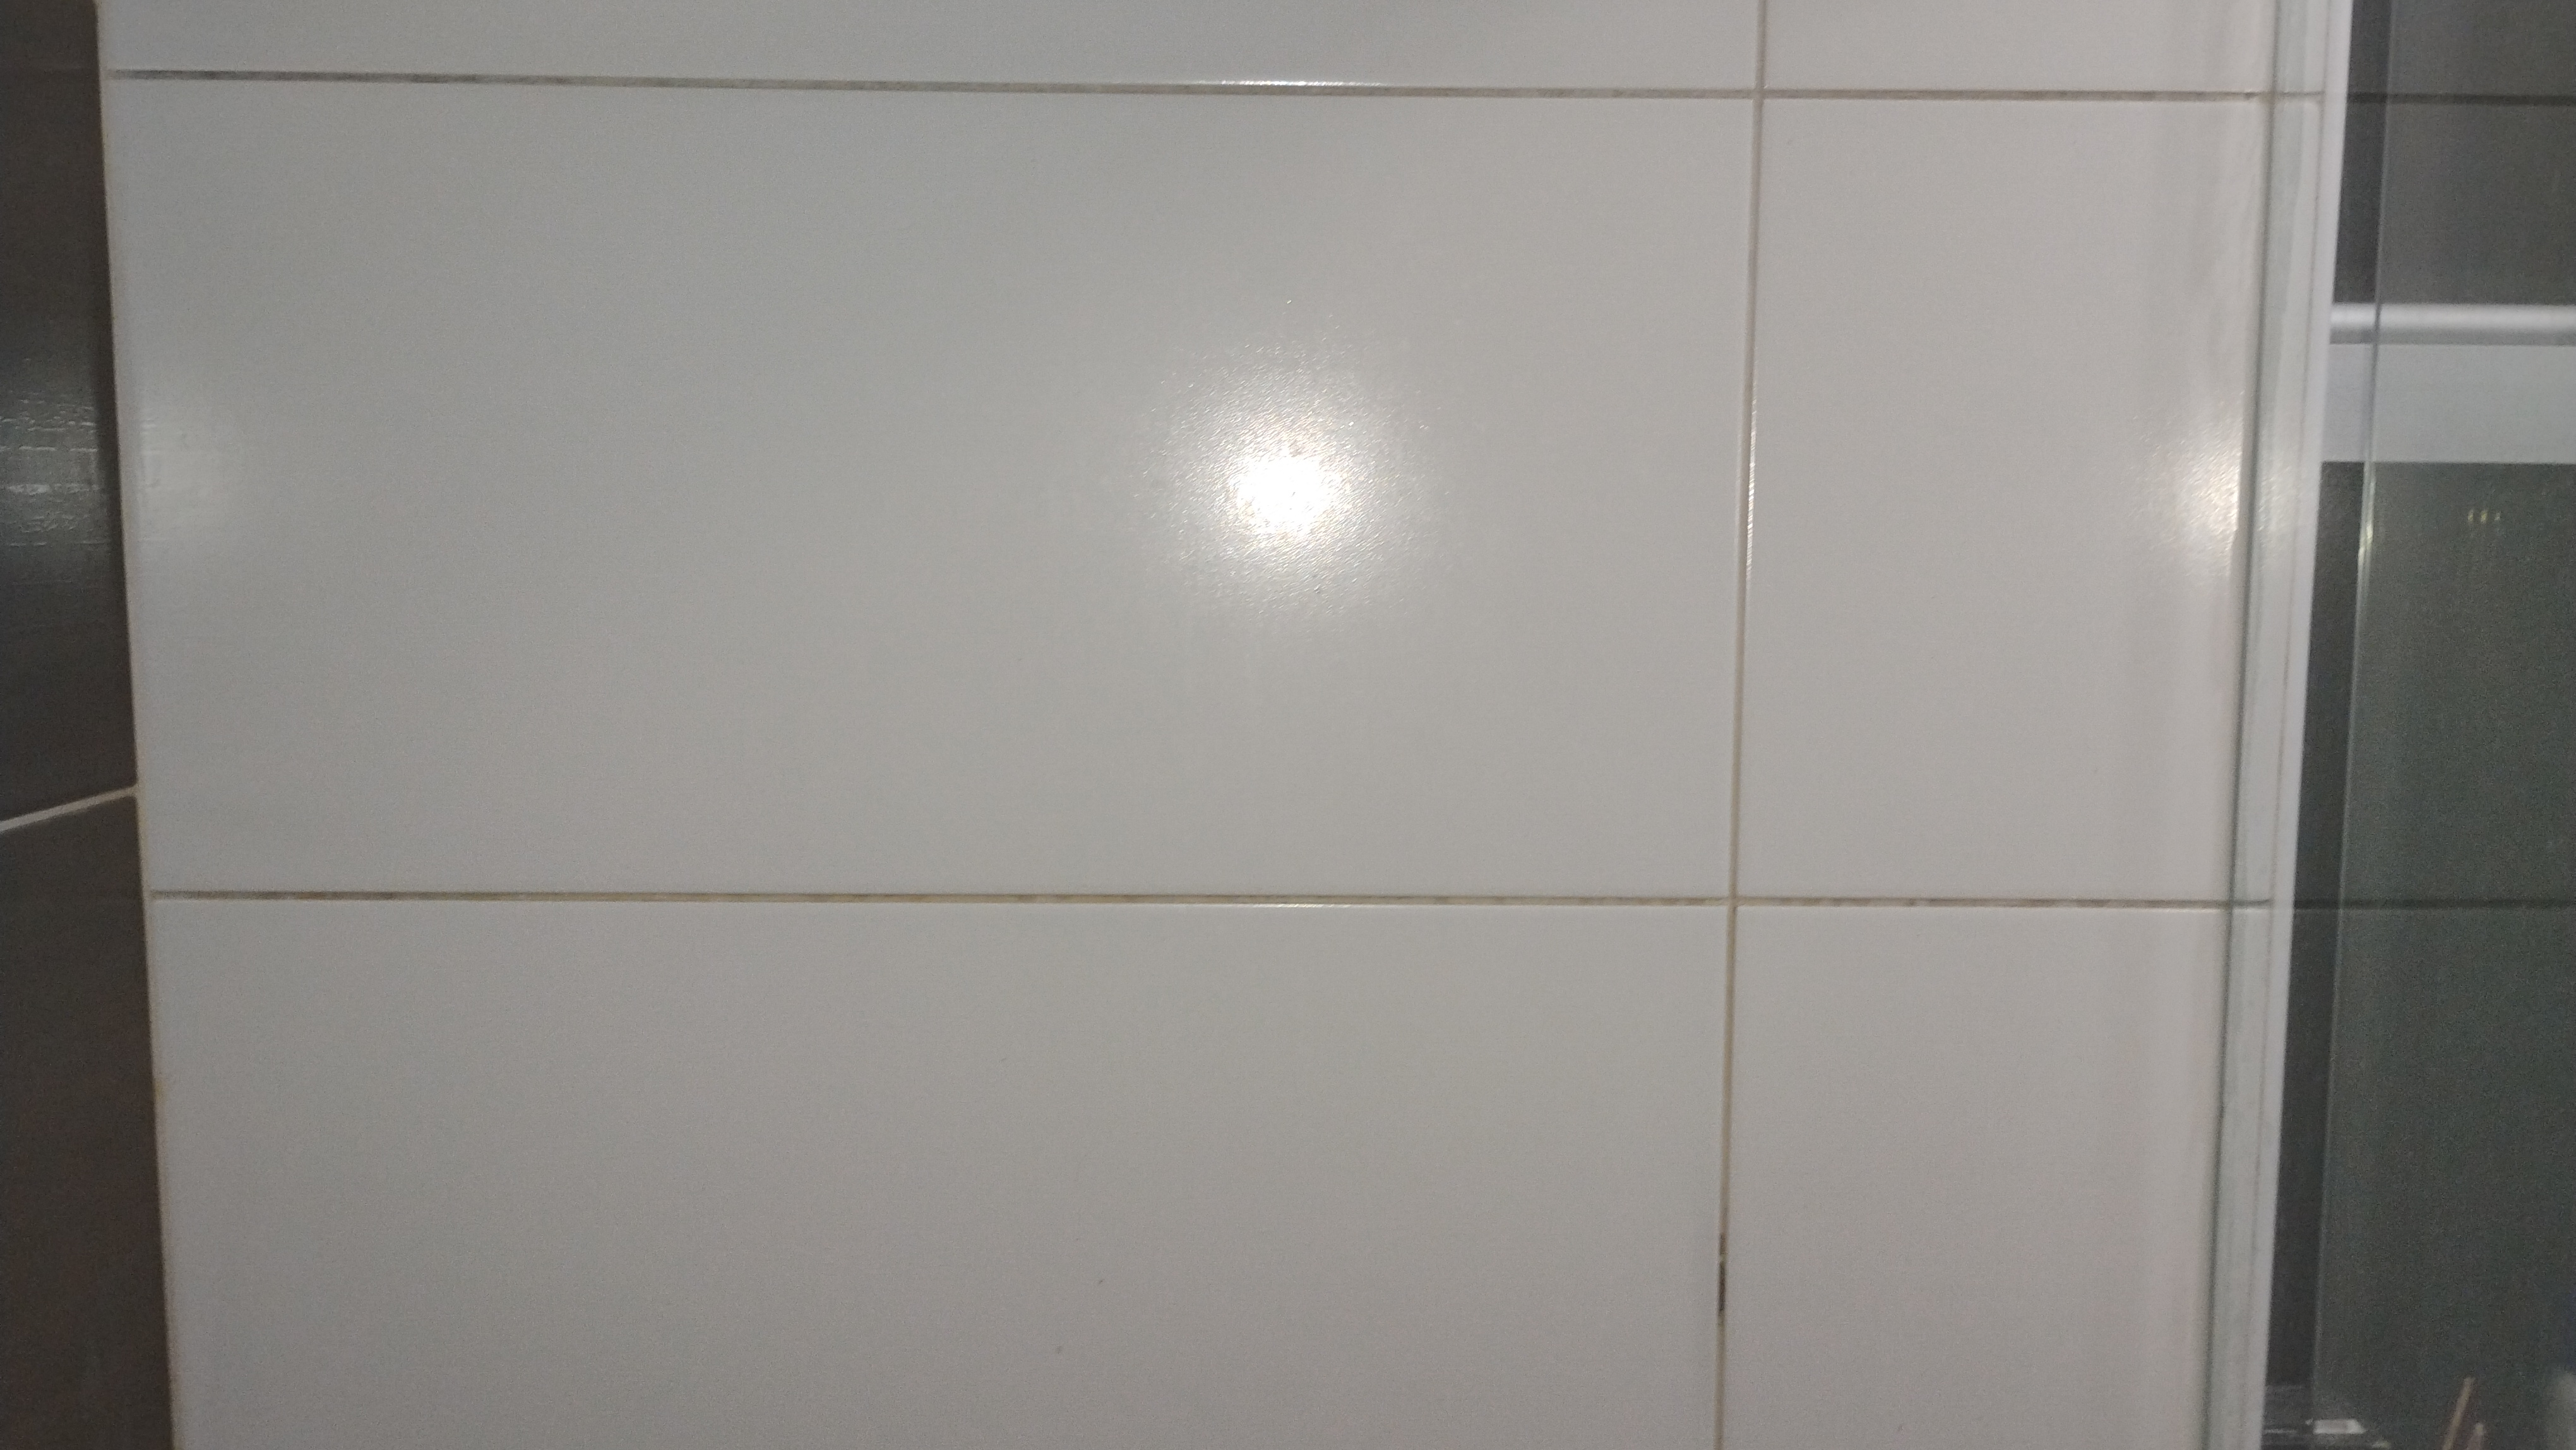
\includegraphics[width=\linewidth]{../img/IMG_20251109_151414054.jpg}\\[2pt]{\footnotesize\color{primary!60!black}Foto~50 -- 15:14:14}} \\[4pt]
\parbox{0.45\textwidth}{\centering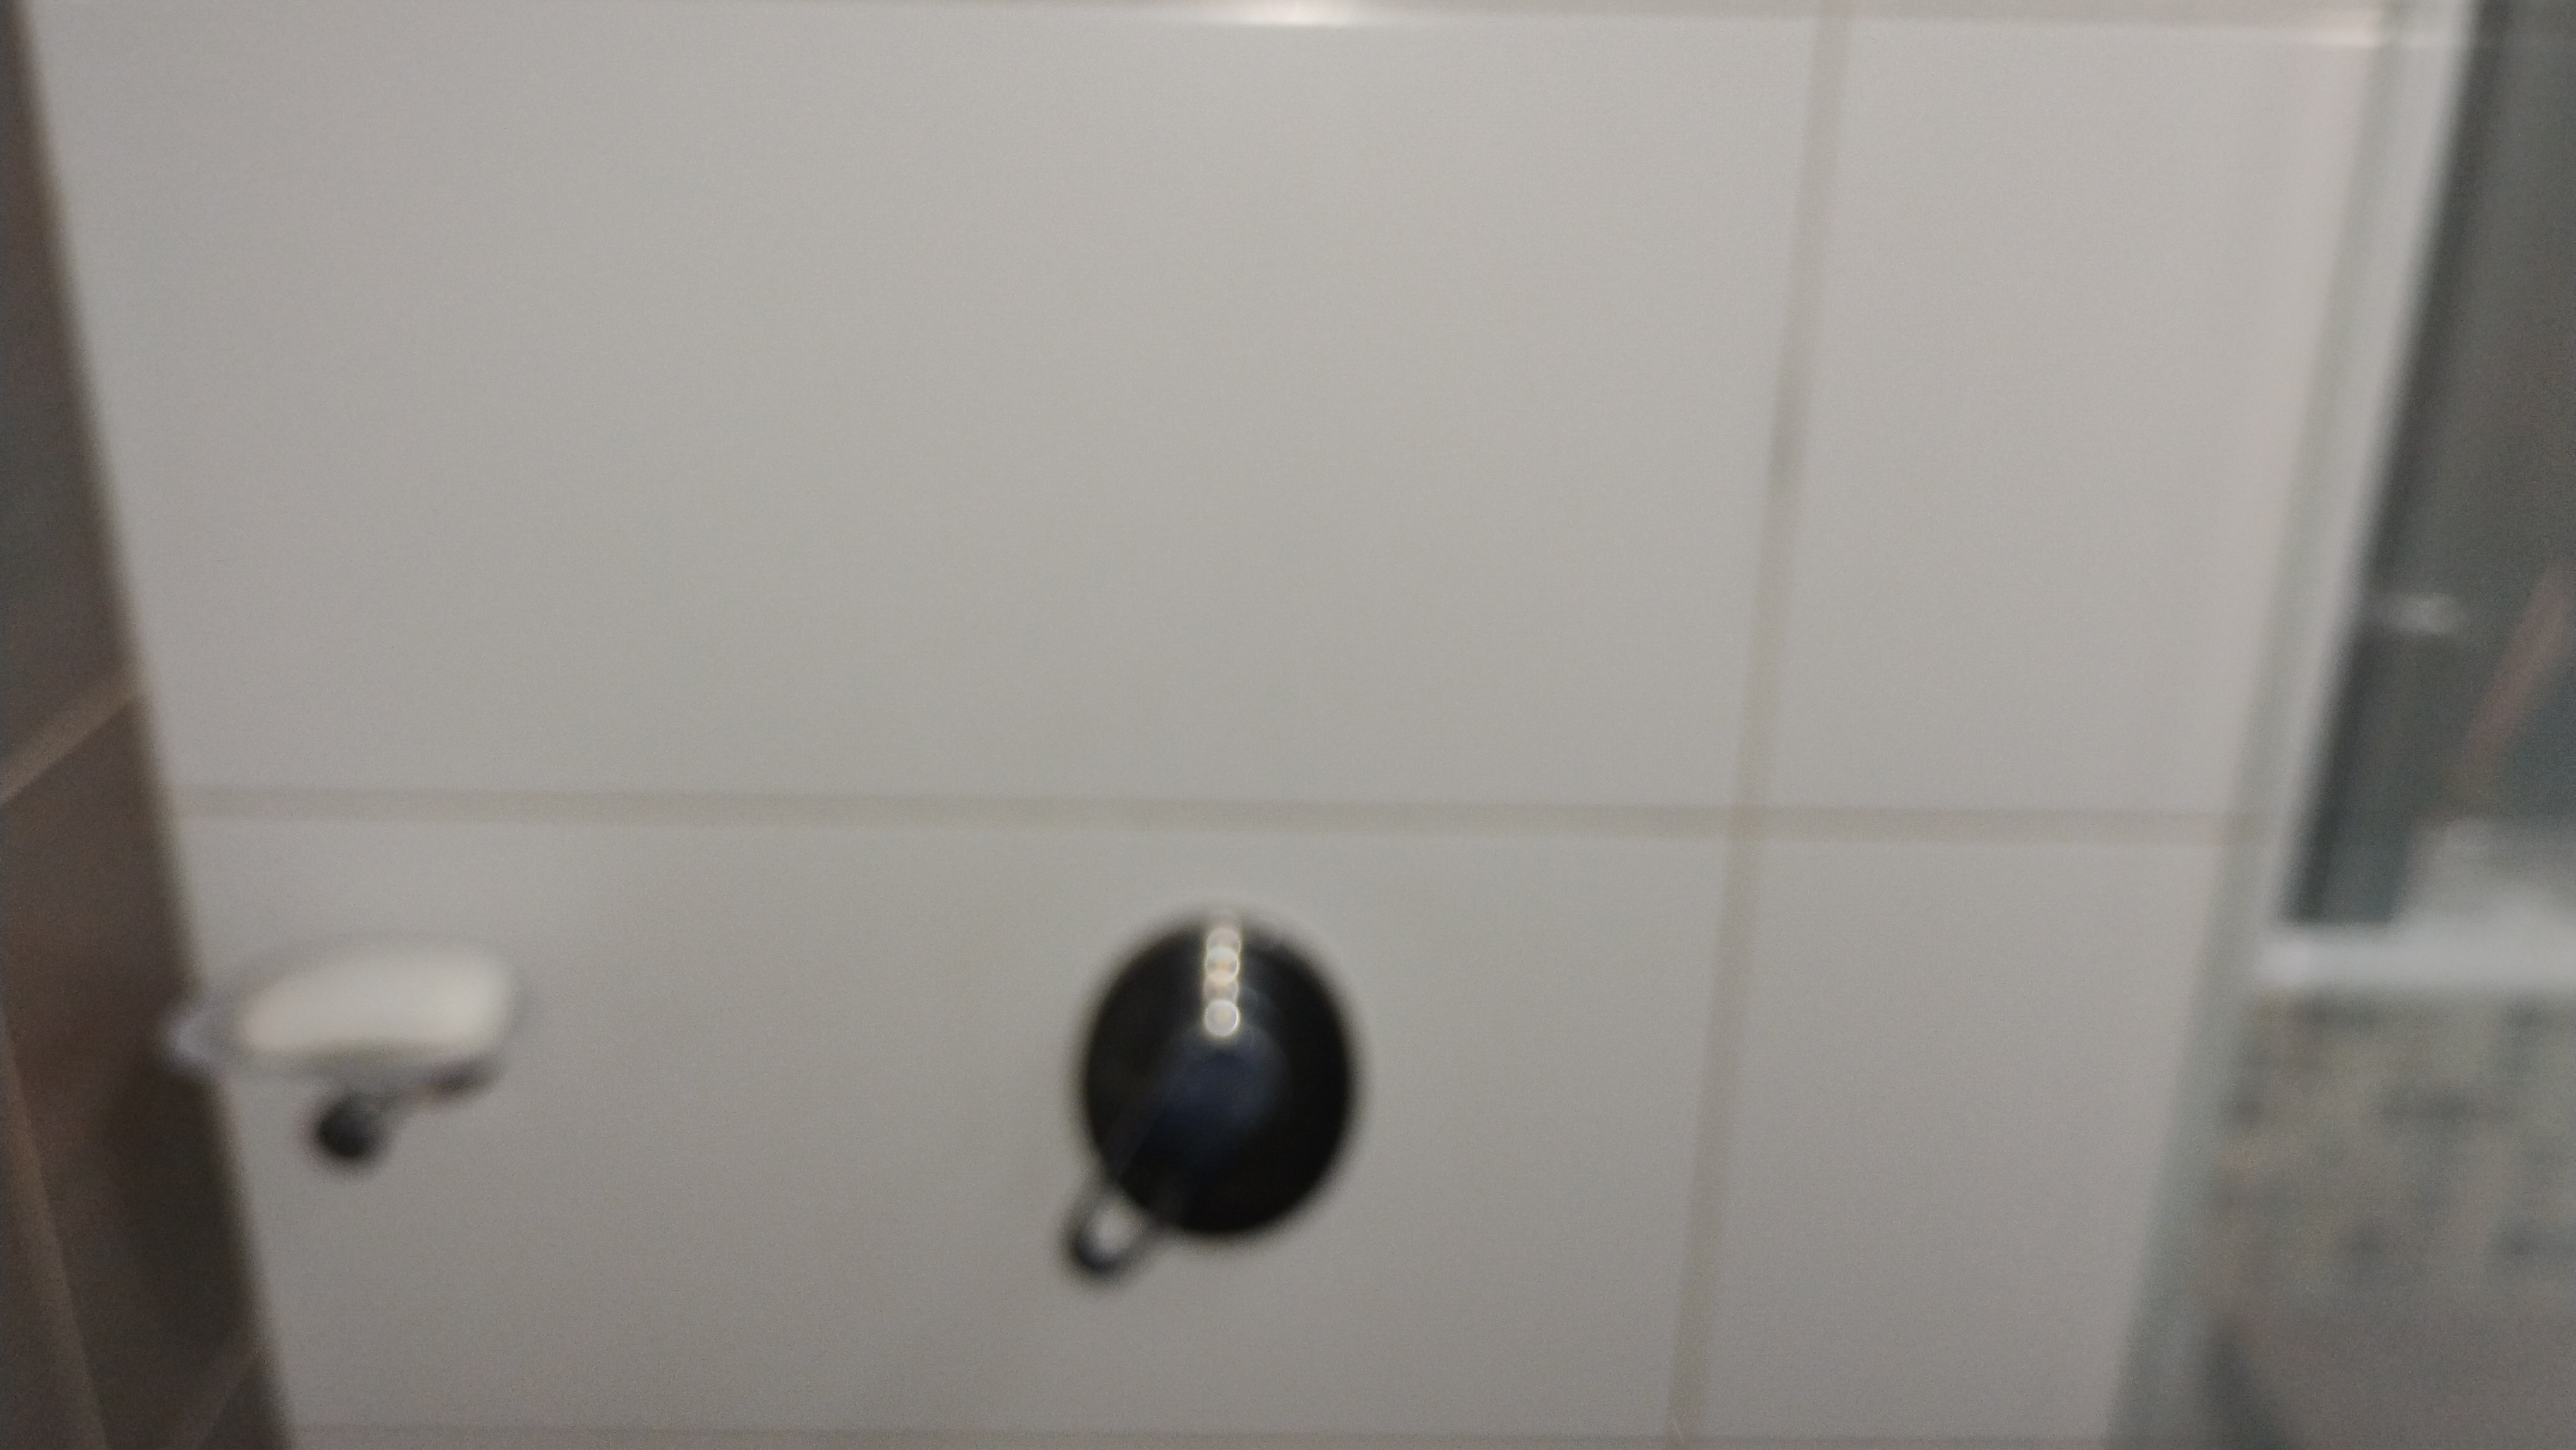
\includegraphics[width=\linewidth]{../img/IMG_20251109_151417083.jpg}\\[2pt]{\footnotesize\color{primary!60!black}Foto~51 -- 15:14:17}} & \parbox{0.45\textwidth}{\centering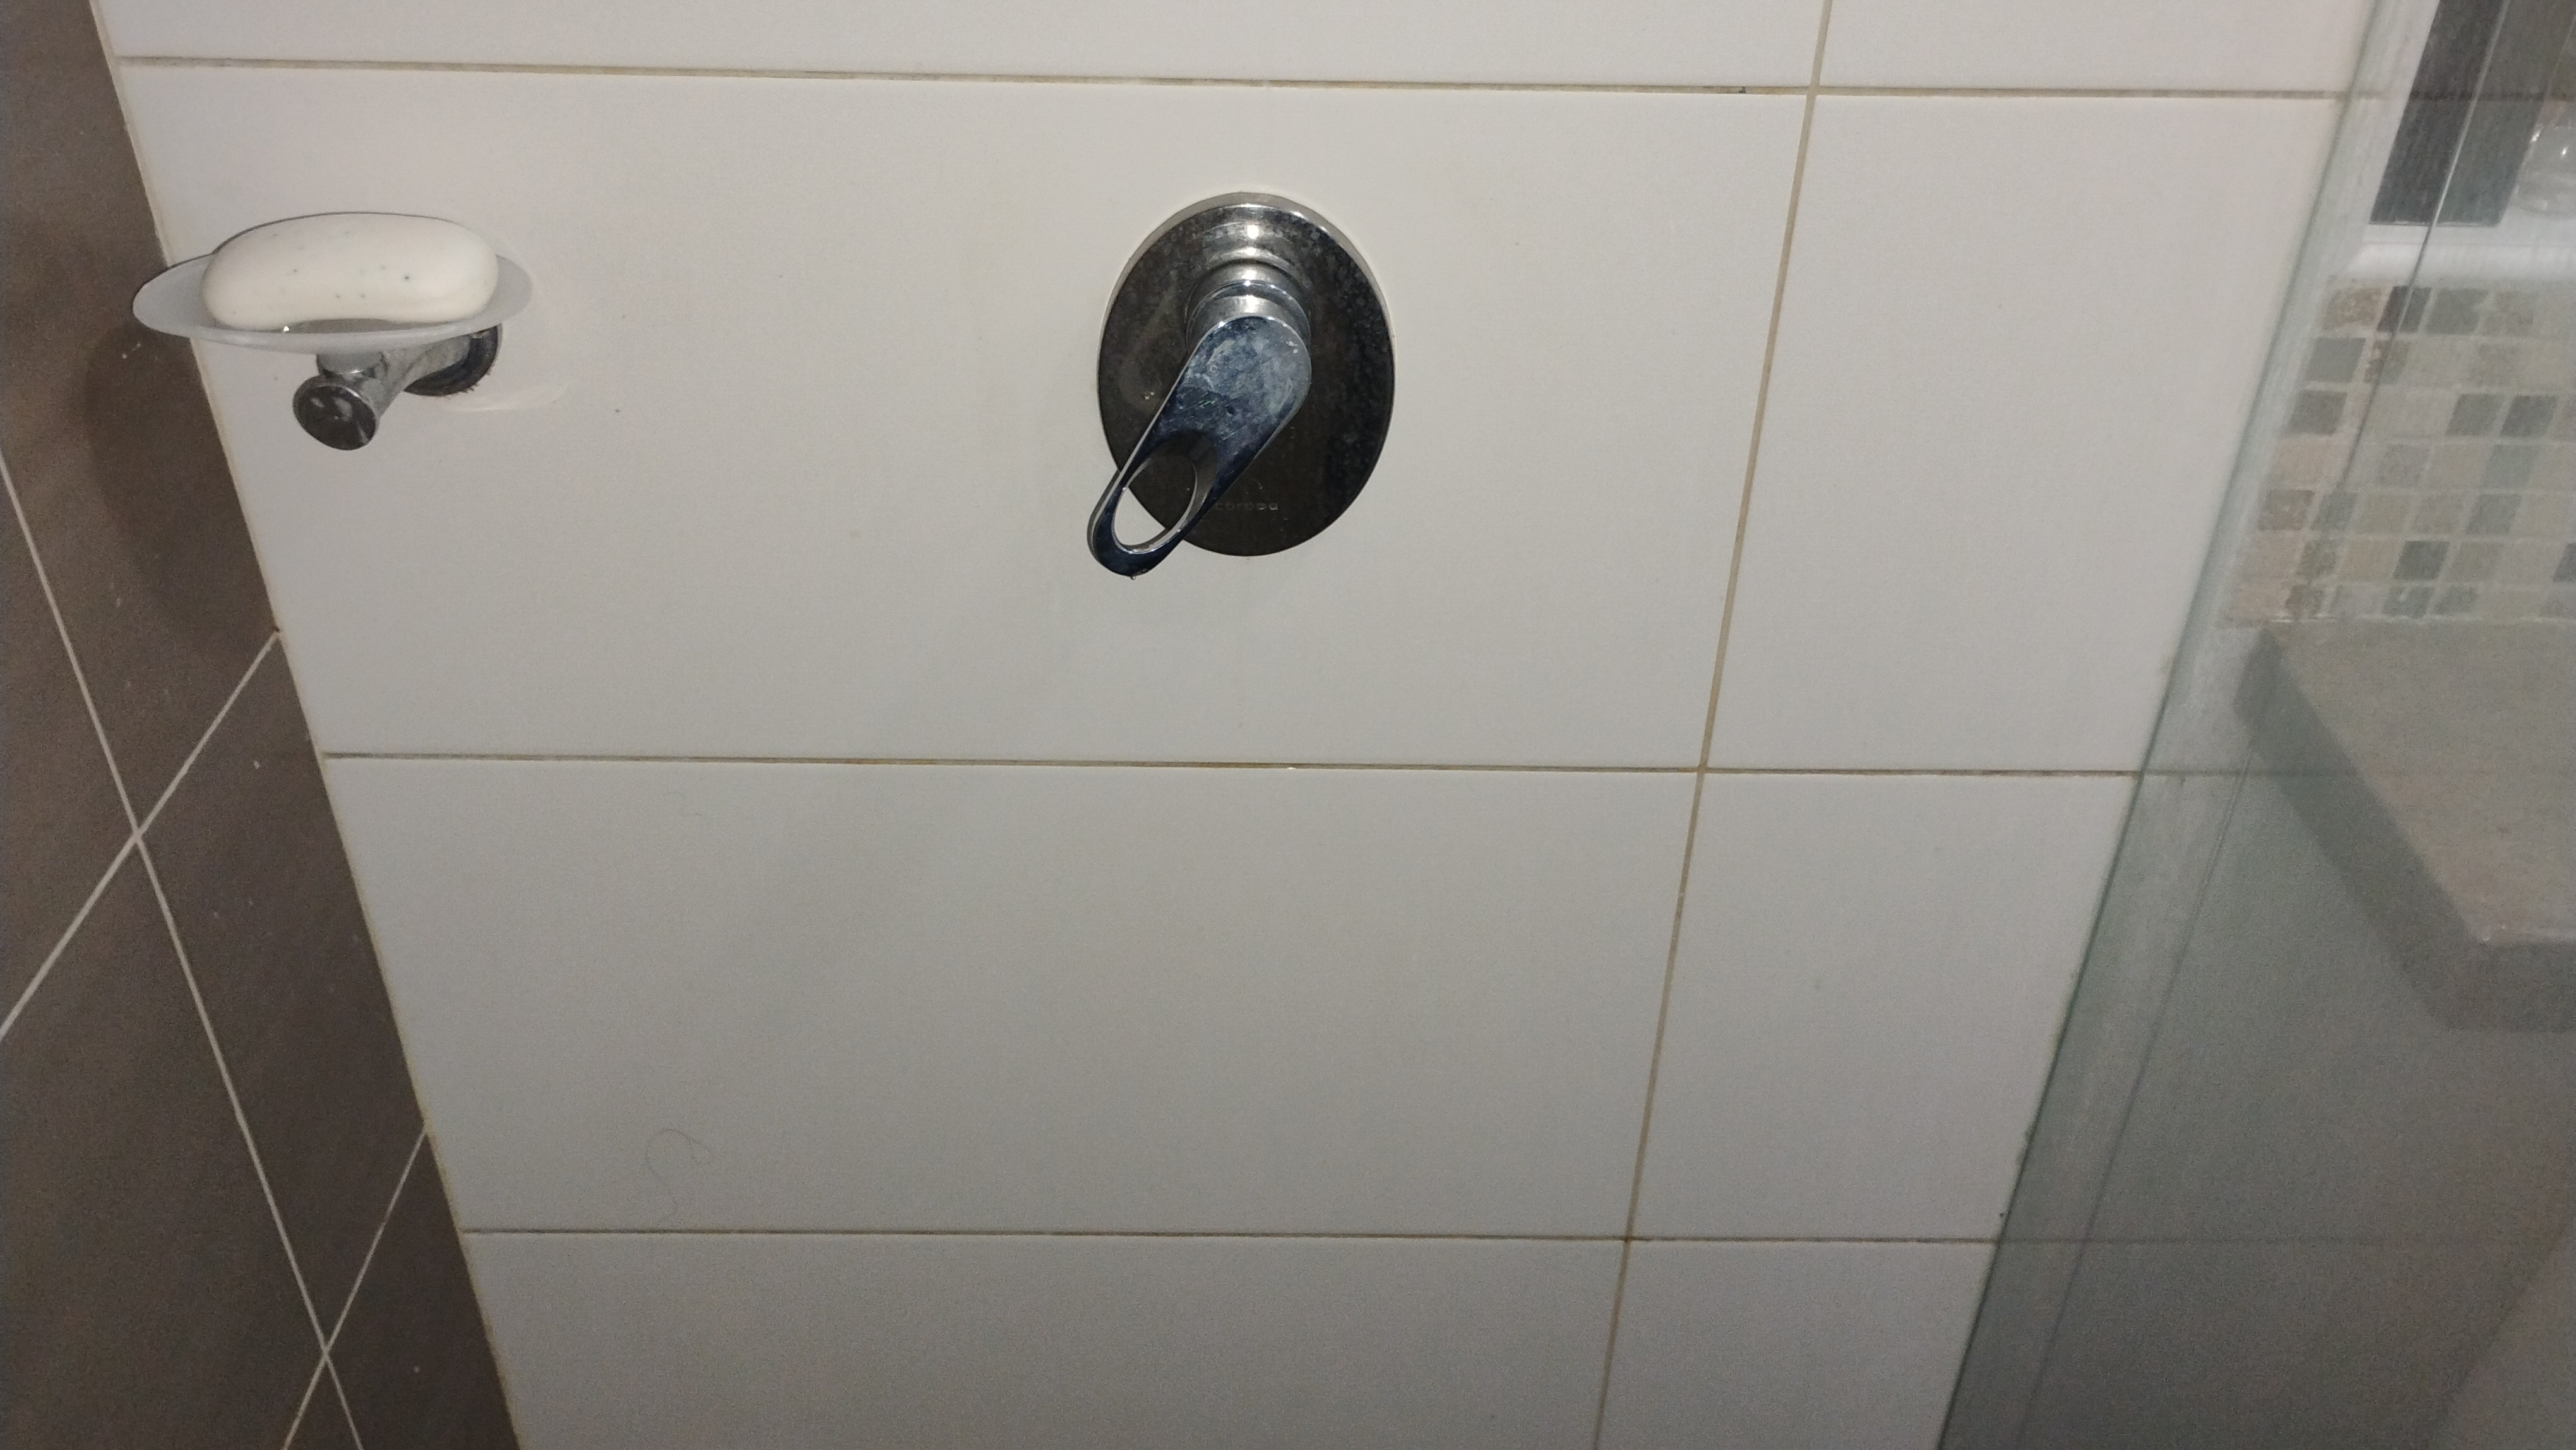
\includegraphics[width=\linewidth]{../img/IMG_20251109_151419682.jpg}\\[2pt]{\footnotesize\color{primary!60!black}Foto~52 -- 15:14:19}} \\[4pt]
\parbox{0.45\textwidth}{\centering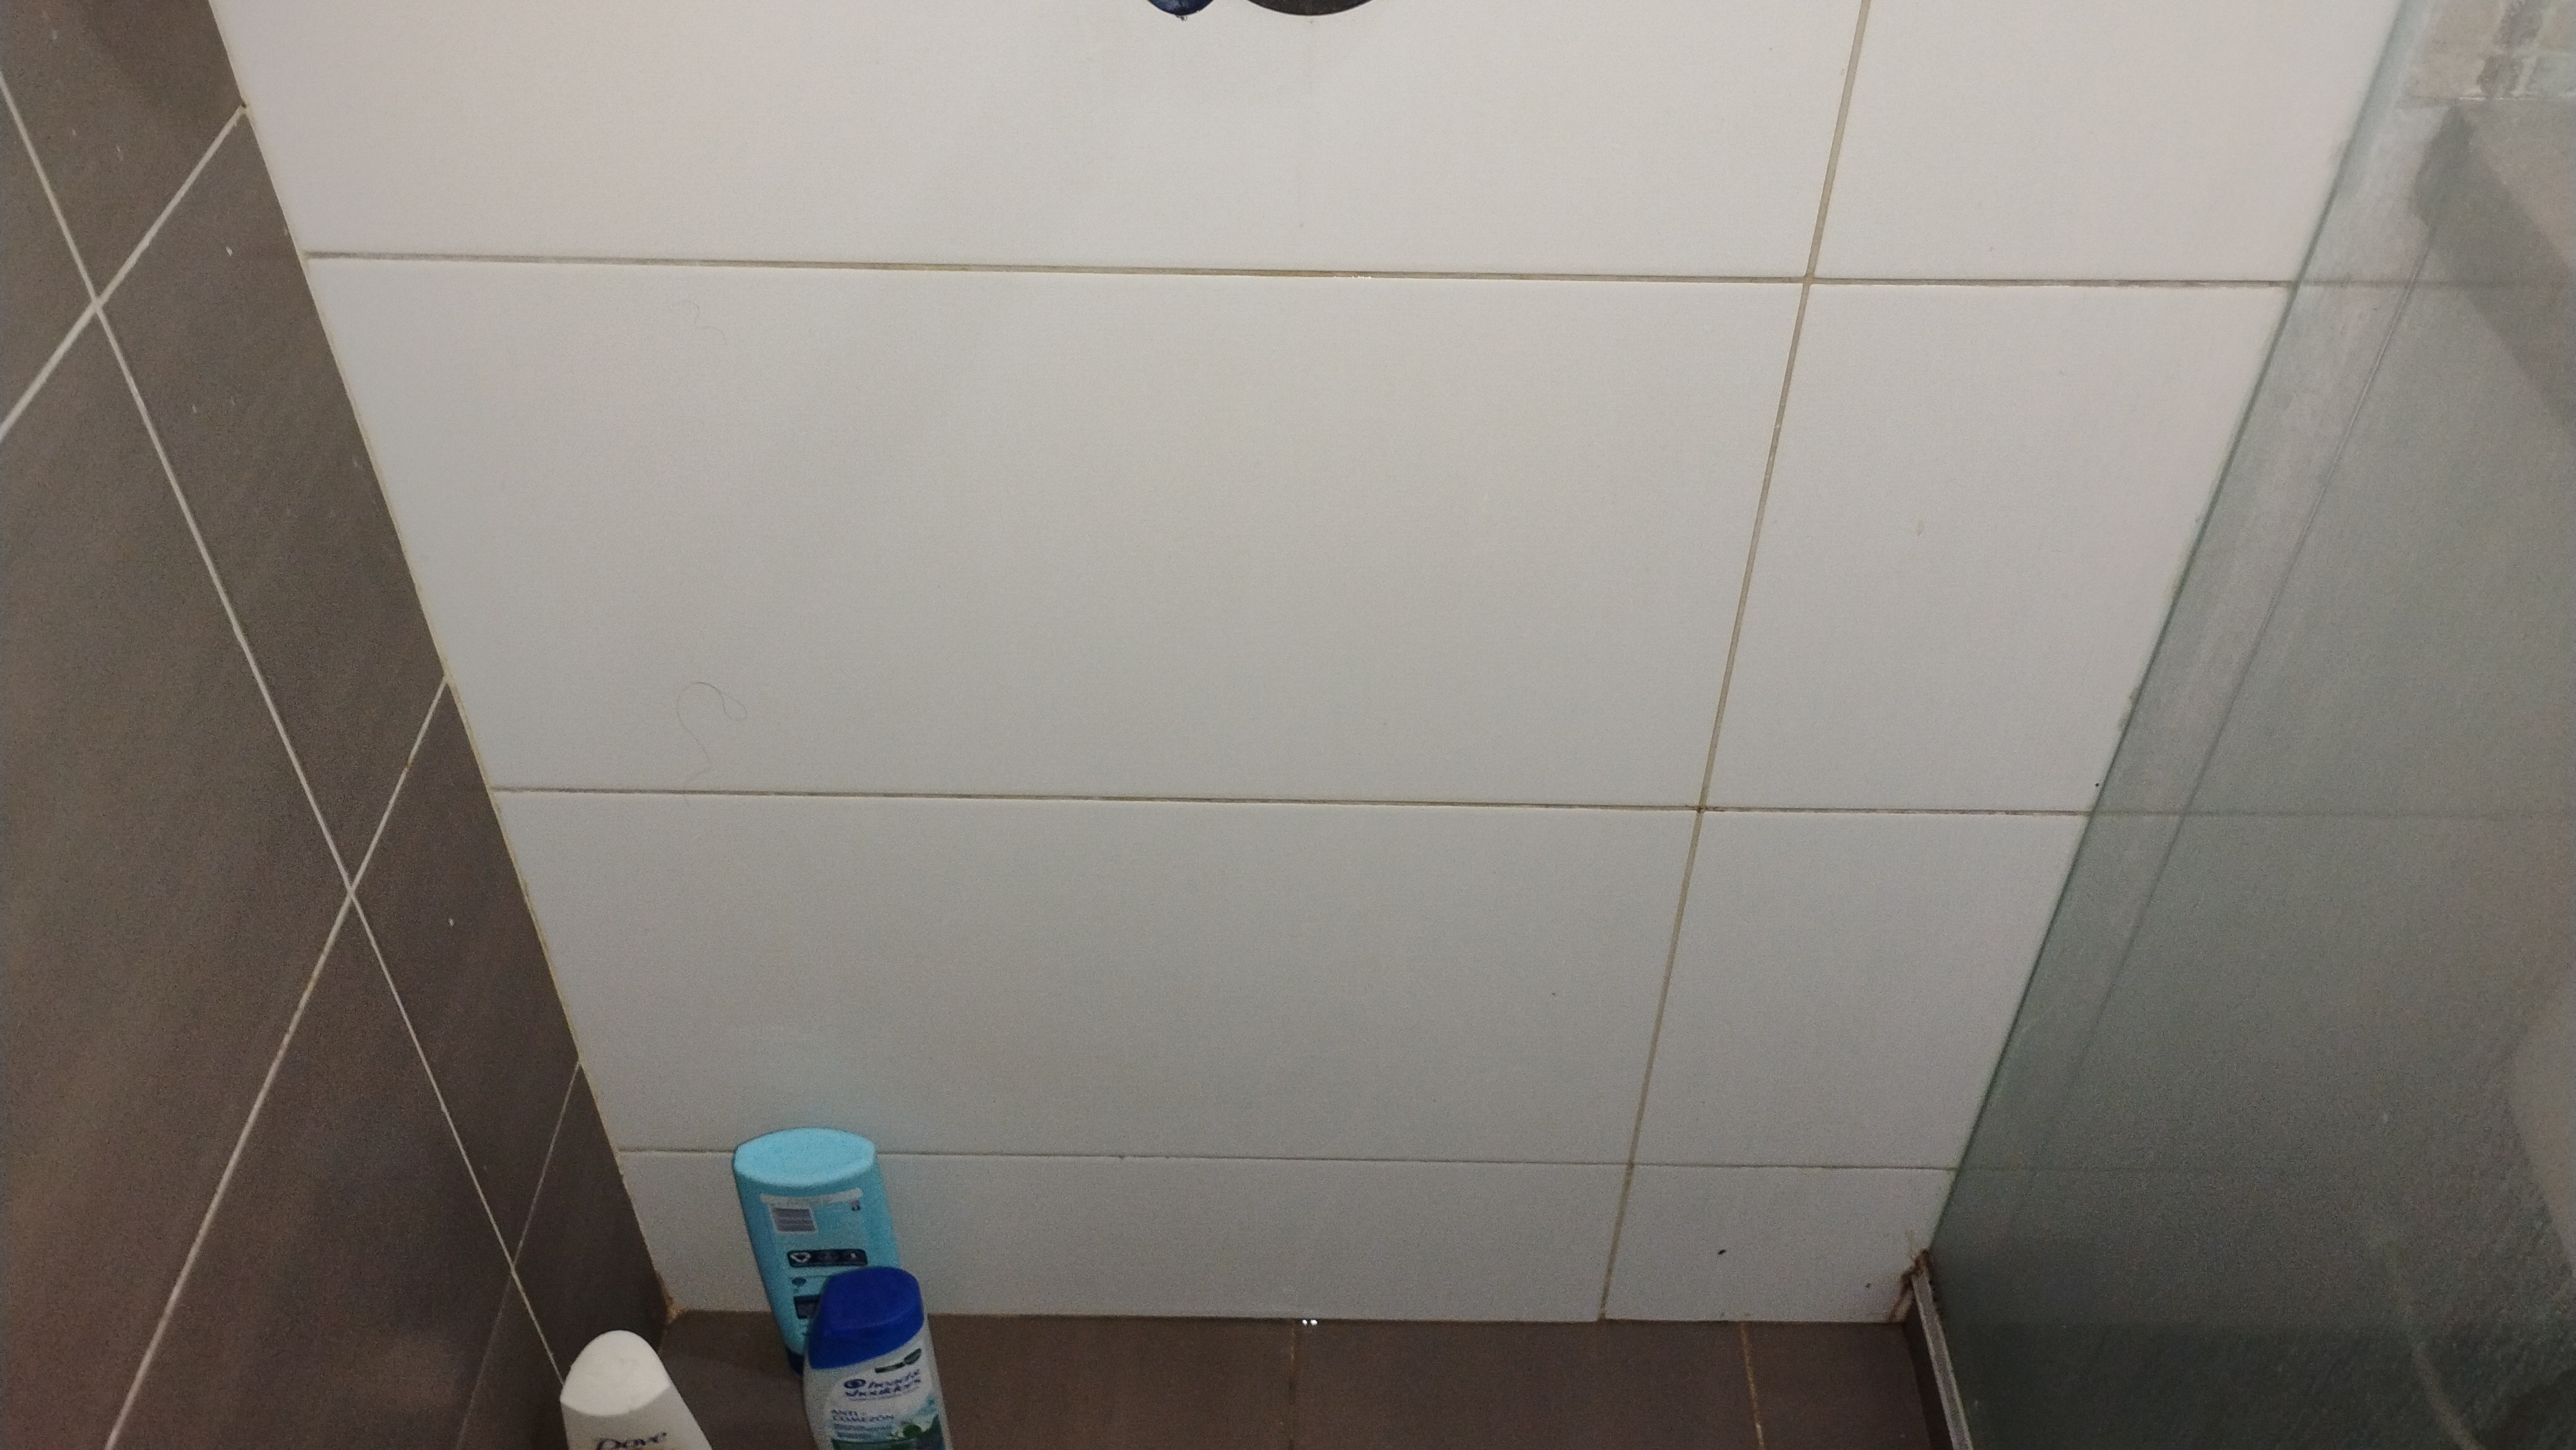
\includegraphics[width=\linewidth]{../img/IMG_20251109_151423568.jpg}\\[2pt]{\footnotesize\color{primary!60!black}Foto~53 -- 15:14:23}} & \parbox{0.45\textwidth}{\centering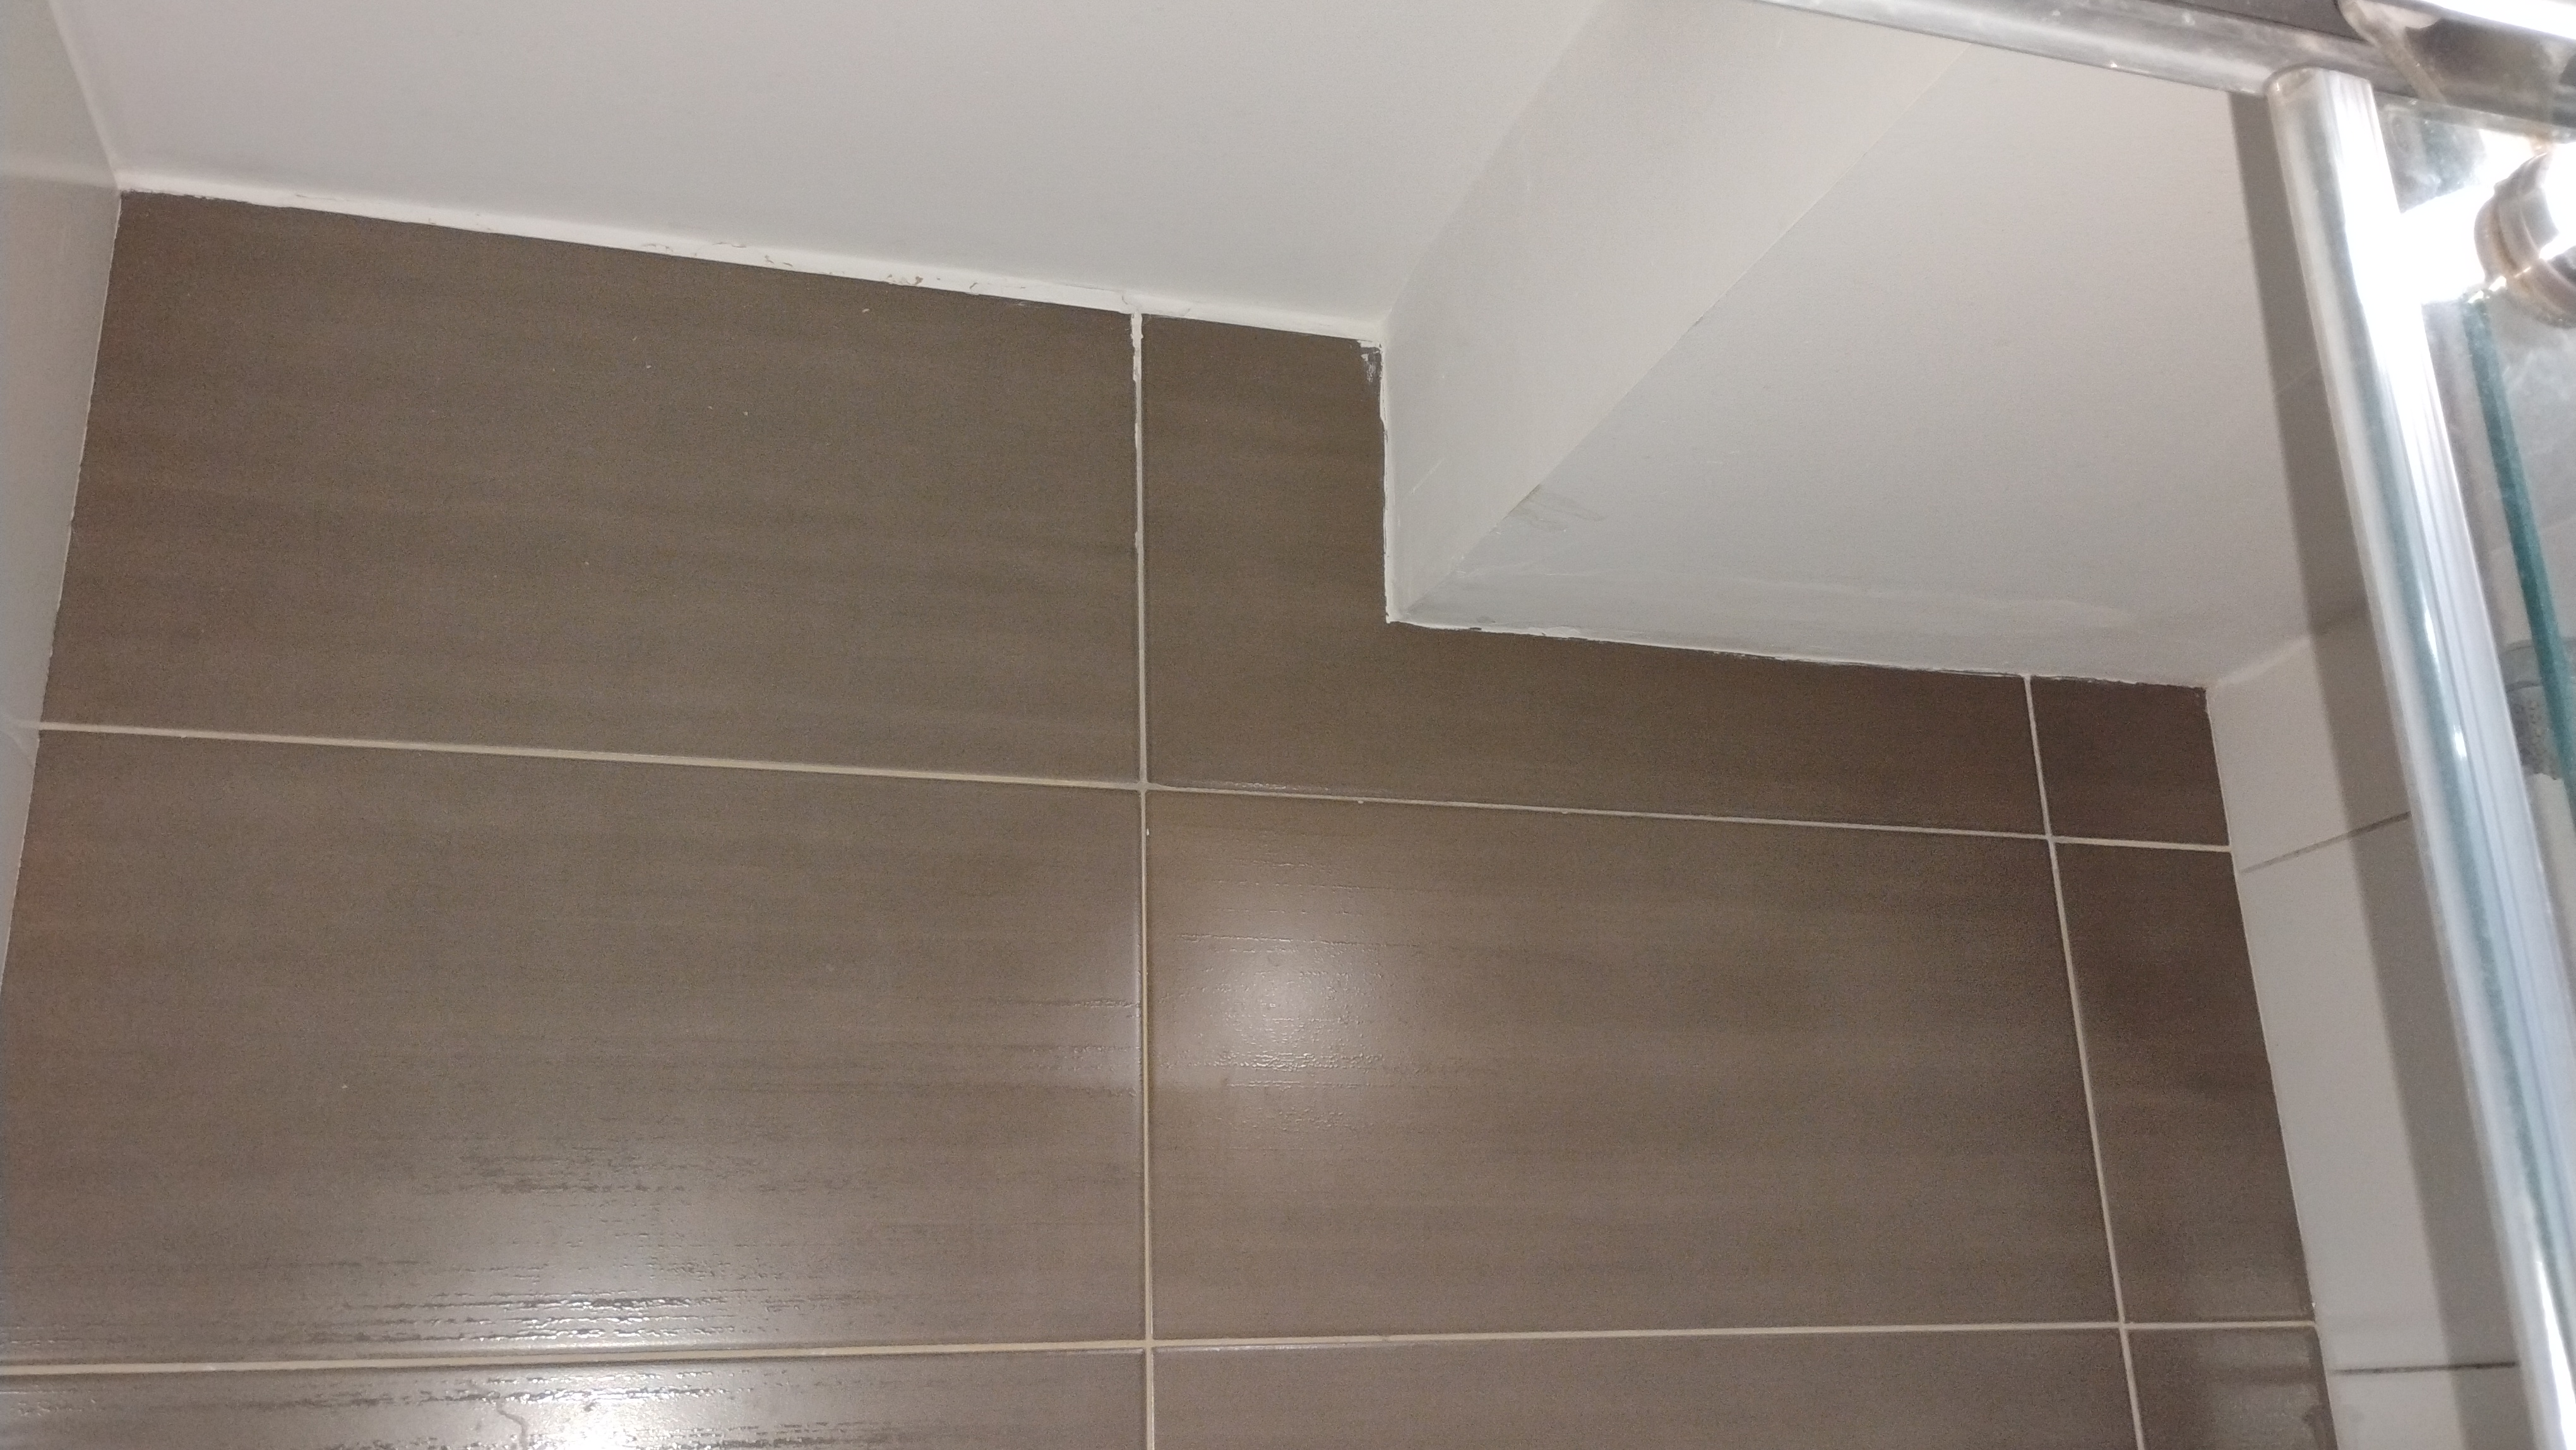
\includegraphics[width=\linewidth]{../img/IMG_20251109_151433653.jpg}\\[2pt]{\footnotesize\color{primary!60!black}Foto~54 -- 15:14:33}} \\[4pt]
\end{tabular}
\caption{Sanitario — Base y Sellos Perimetrales: Fotos 49 al 54.}\end{figure}
\newpage
\begin{figure}[H]
\centering
\begin{tabular}{cc}
\parbox{0.45\textwidth}{\centering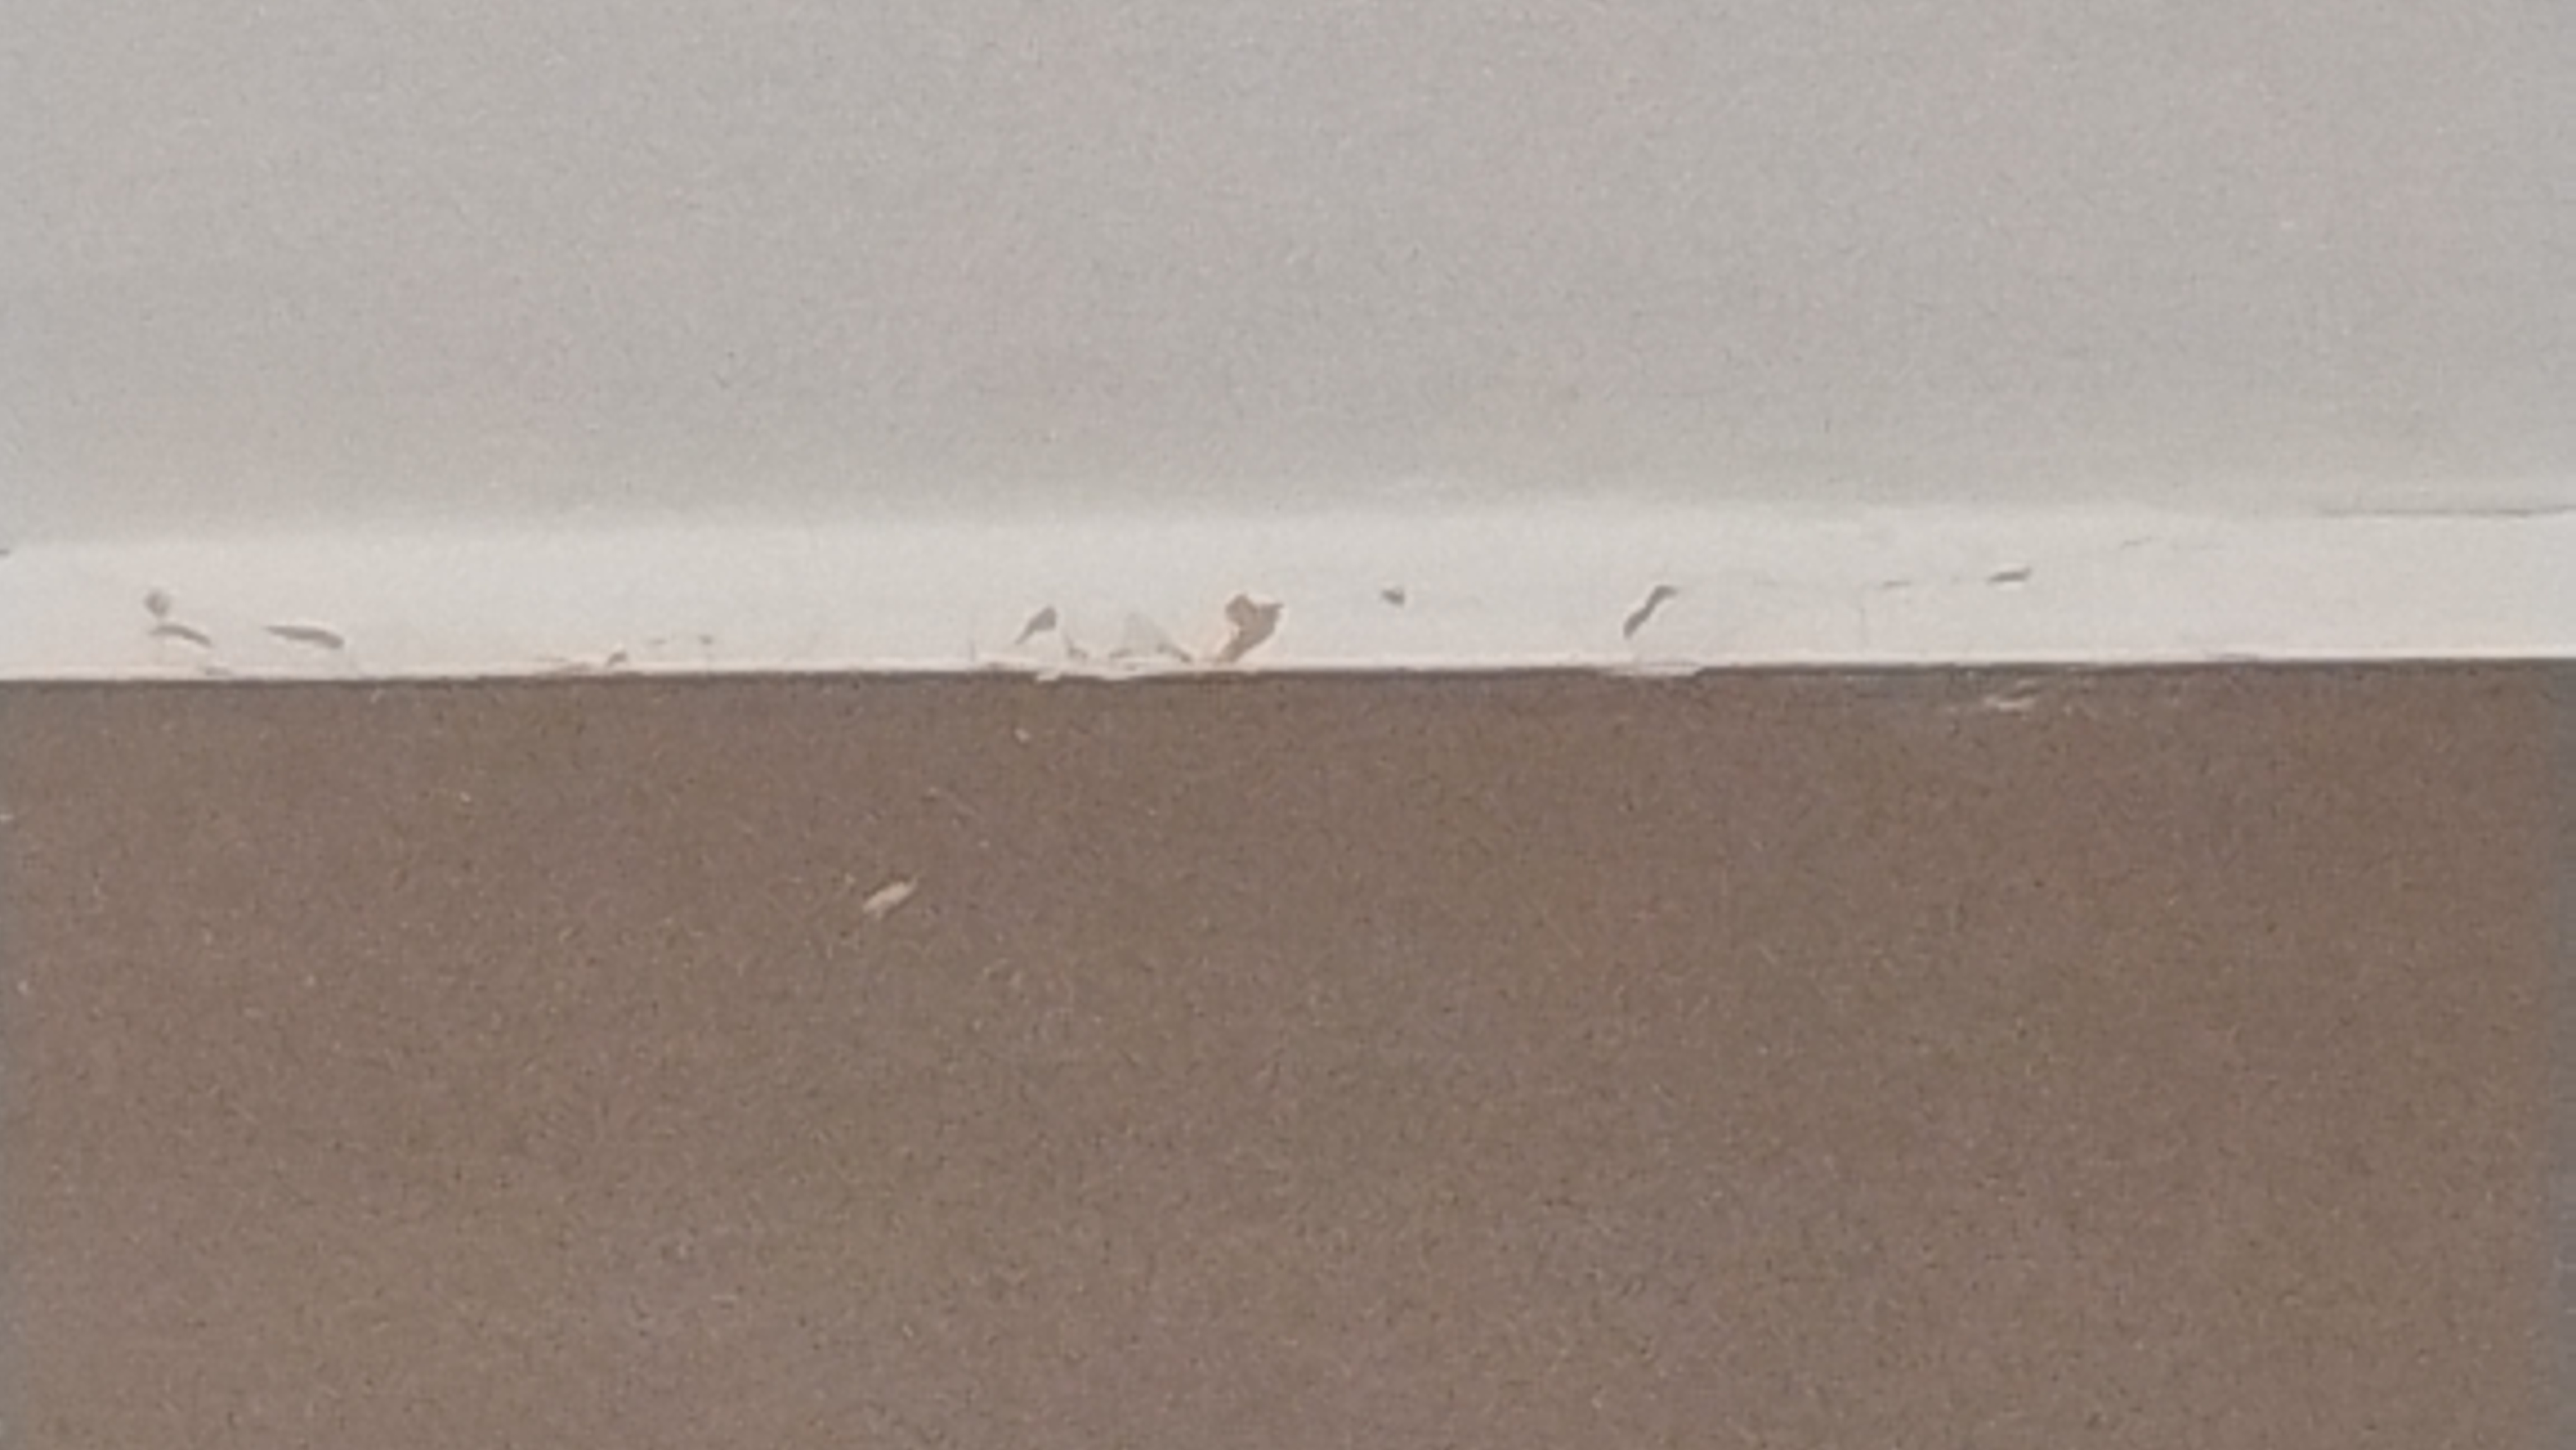
\includegraphics[width=\linewidth]{../img/IMG_20251109_151448470.jpg}\\[2pt]{\footnotesize\color{primary!60!black}Foto~55 -- 15:14:48}} & \parbox{0.45\textwidth}{\centering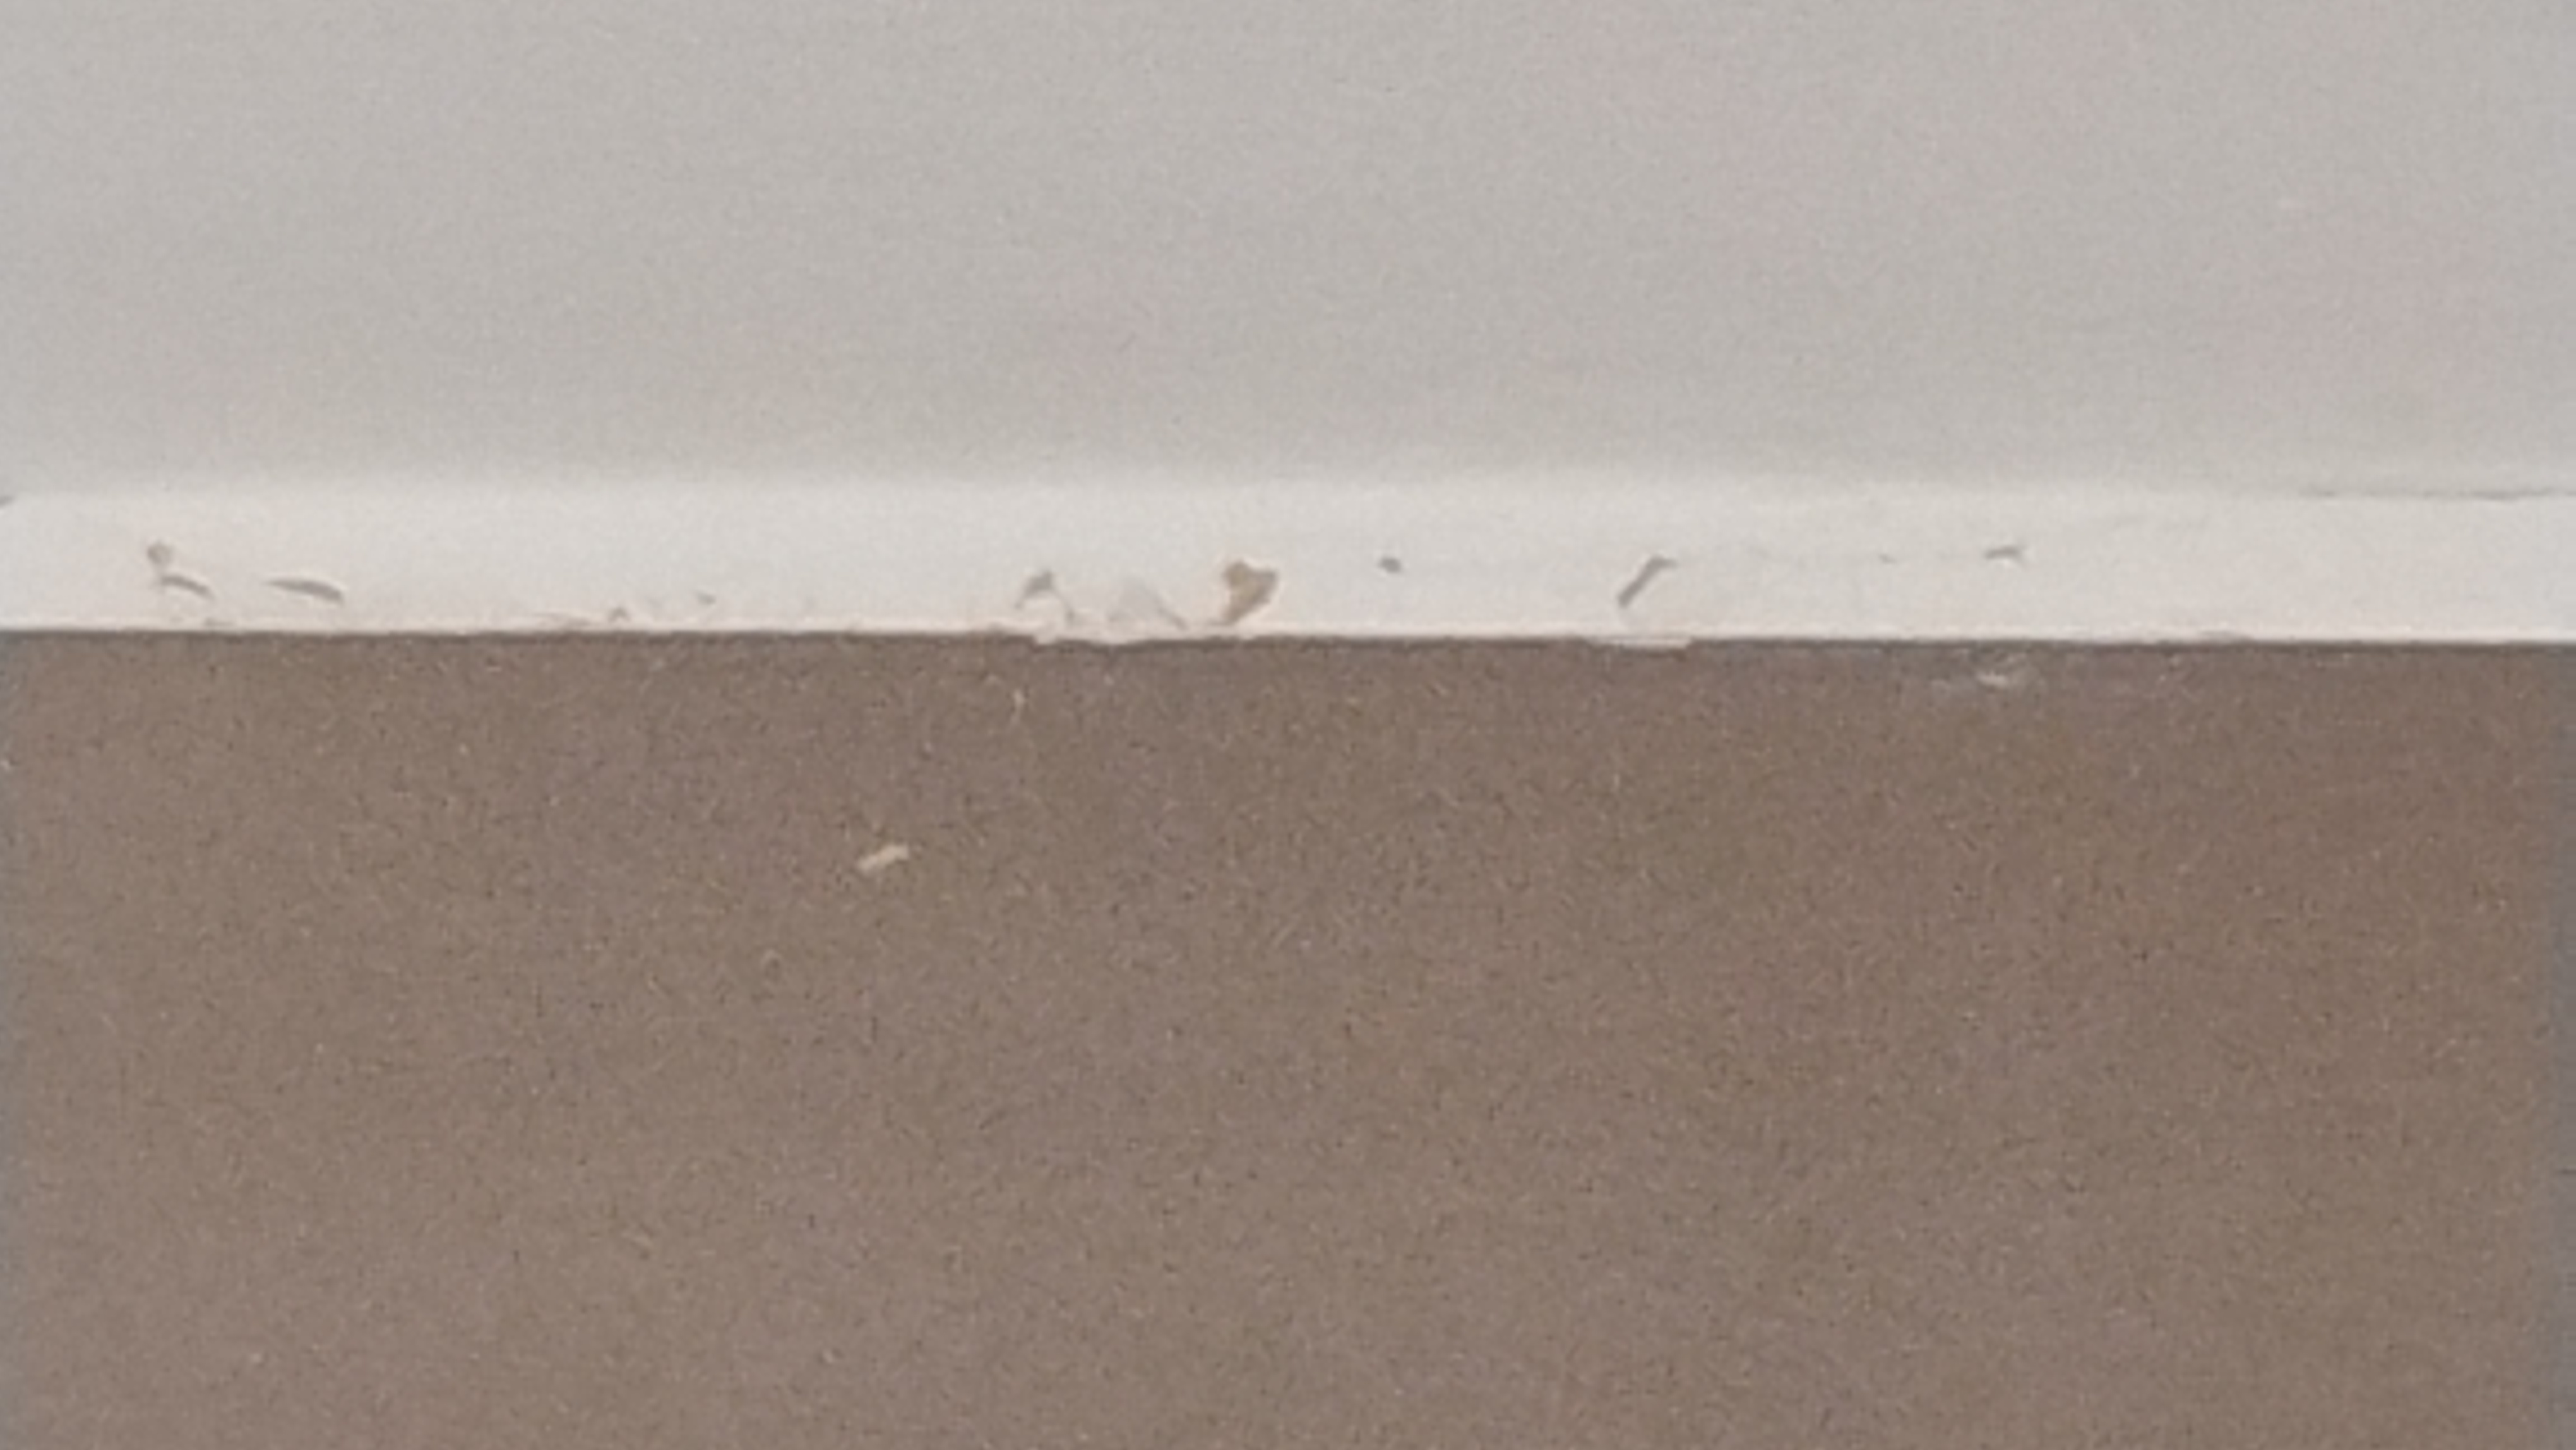
\includegraphics[width=\linewidth]{../img/IMG_20251109_151451115.jpg}\\[2pt]{\footnotesize\color{primary!60!black}Foto~56 -- 15:14:51}} \\[4pt]
\parbox{0.45\textwidth}{\centering
\includegraphics[width=\linewidth]{../img/IMG_20251109_151609741.jpg}\\[2pt]{\footnotesize\color{primary!60!black}Foto~57 -- 15:16:09}} & \parbox{0.45\textwidth}{\centering
\includegraphics[width=\linewidth]{../img/IMG_20251109_151613111.jpg}\\[2pt]{\footnotesize\color{primary!60!black}Foto~58 -- 15:16:13}} \\[4pt]
\parbox{0.45\textwidth}{\centering
\includegraphics[width=\linewidth]{../img/IMG_20251109_151616802.jpg}\\[2pt]{\footnotesize\color{primary!60!black}Foto~59 -- 15:16:16}} & \parbox{0.45\textwidth}{\centering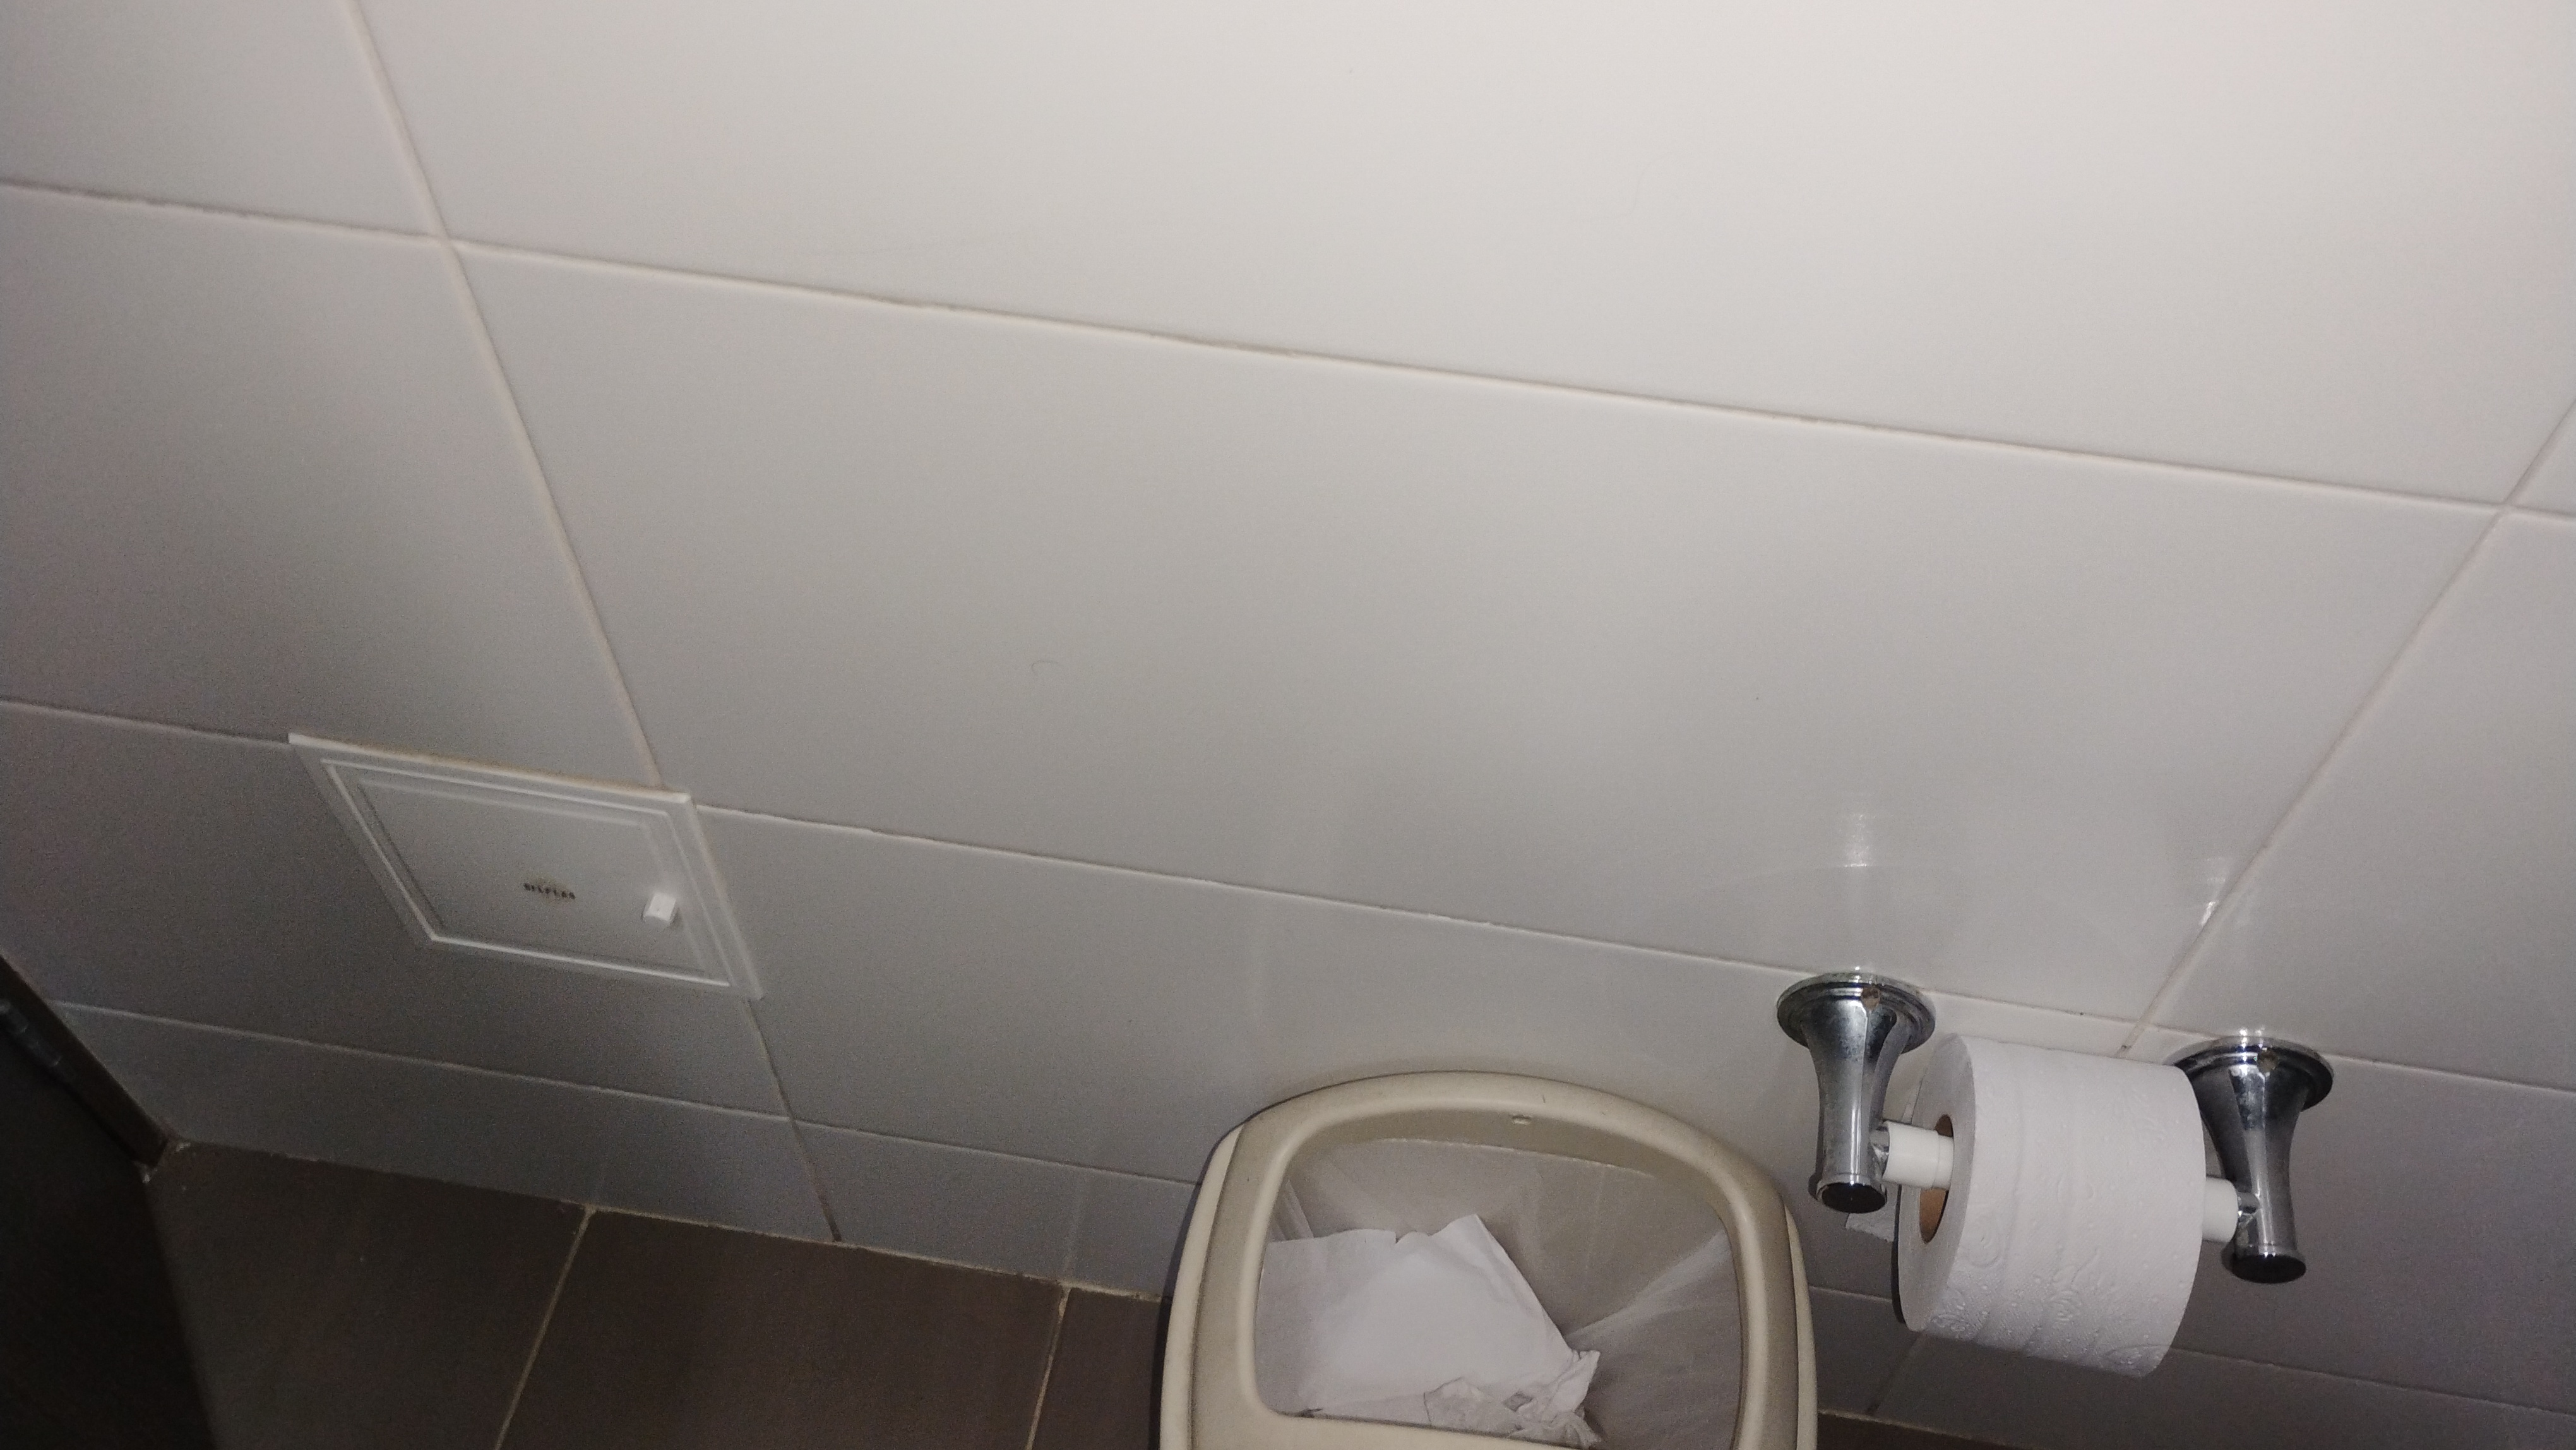
\includegraphics[width=\linewidth]{../img/IMG_20251109_151620204.jpg}\\[2pt]{\footnotesize\color{primary!60!black}Foto~60 -- 15:16:20}} \\[4pt]
\end{tabular}
\caption{Revestimiento de Piso — Lechada, Boquillas y Cavidades: Fotos 55 al 60.}\end{figure}
\newpage
\begin{figure}[H]
\centering
\begin{tabular}{cc}
\parbox{0.45\textwidth}{\centering
\includegraphics[width=\linewidth]{../img/IMG_20251109_151623731.jpg}\\[2pt]{\footnotesize\color{primary!60!black}Foto~61 -- 15:16:23}} & \parbox{0.45\textwidth}{\centering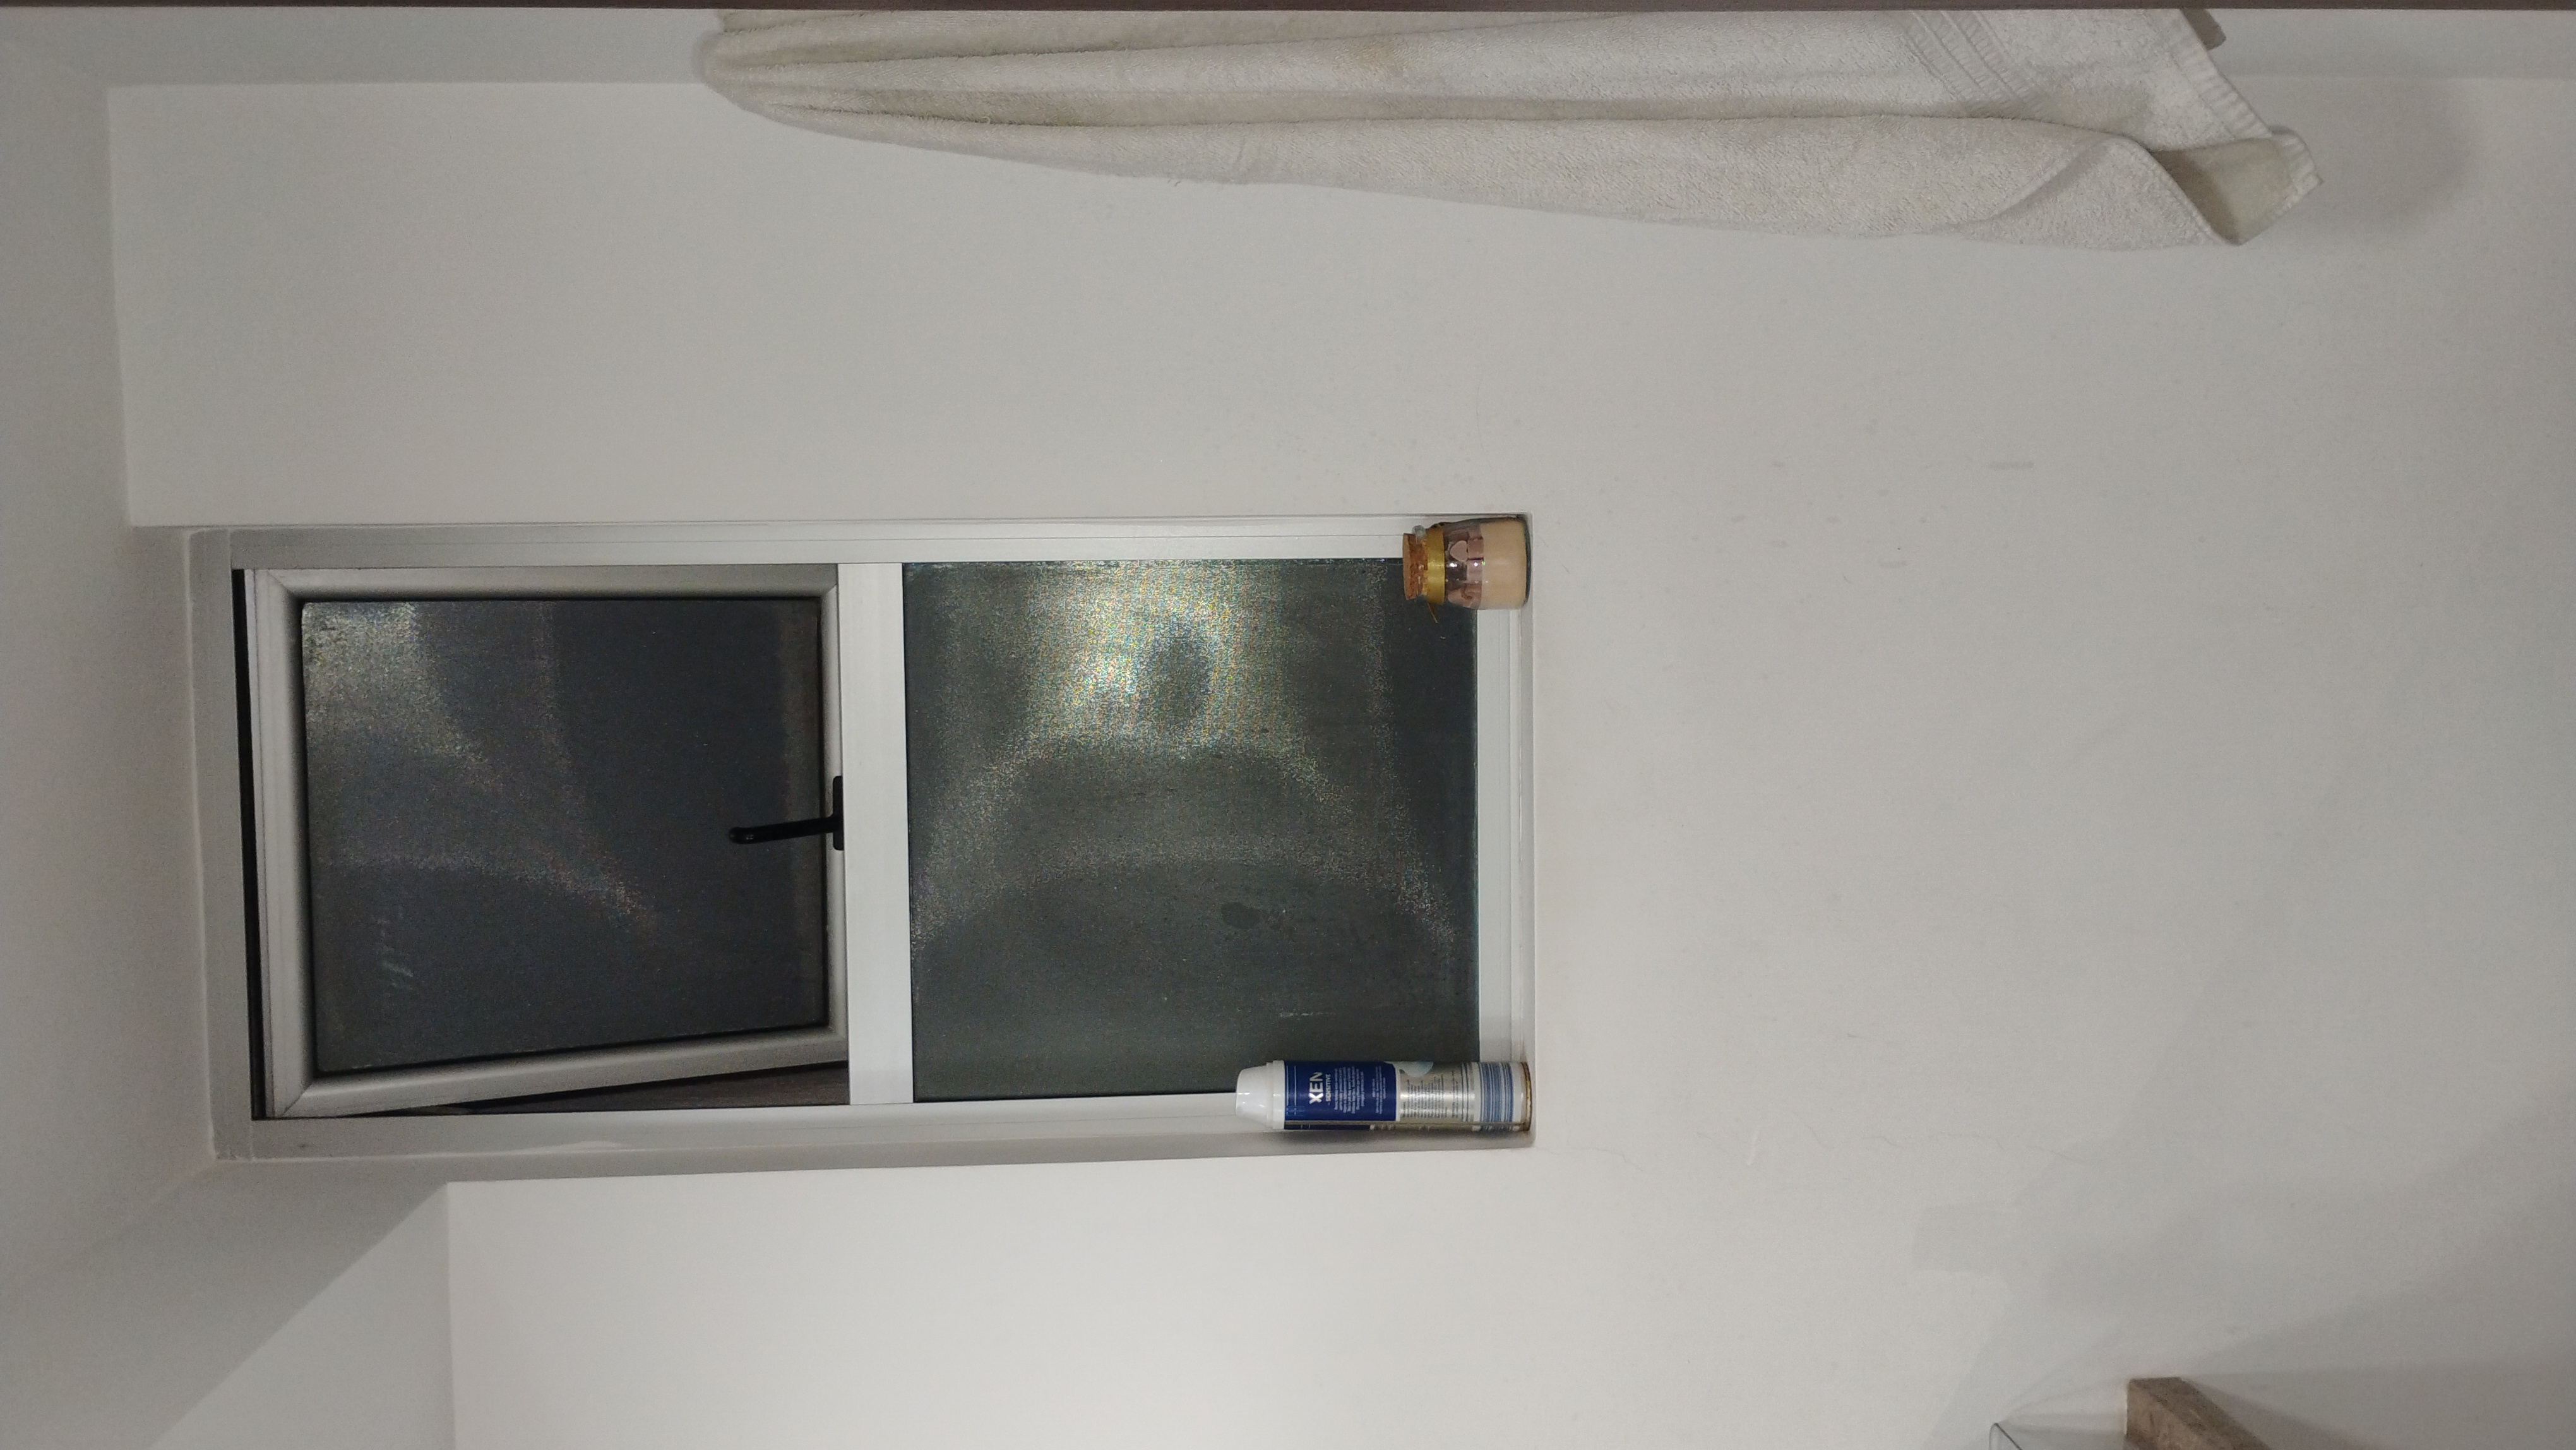
\includegraphics[width=\linewidth]{../img/IMG_20251109_151725563.jpg}\\[2pt]{\footnotesize\color{primary!60!black}Foto~62 -- 15:17:25}} \\[4pt]
\parbox{0.45\textwidth}{\centering
\includegraphics[width=\linewidth]{../img/IMG_20251109_151742445.jpg}\\[2pt]{\footnotesize\color{primary!60!black}Foto~63 -- 15:17:42}} & \parbox{0.45\textwidth}{\centering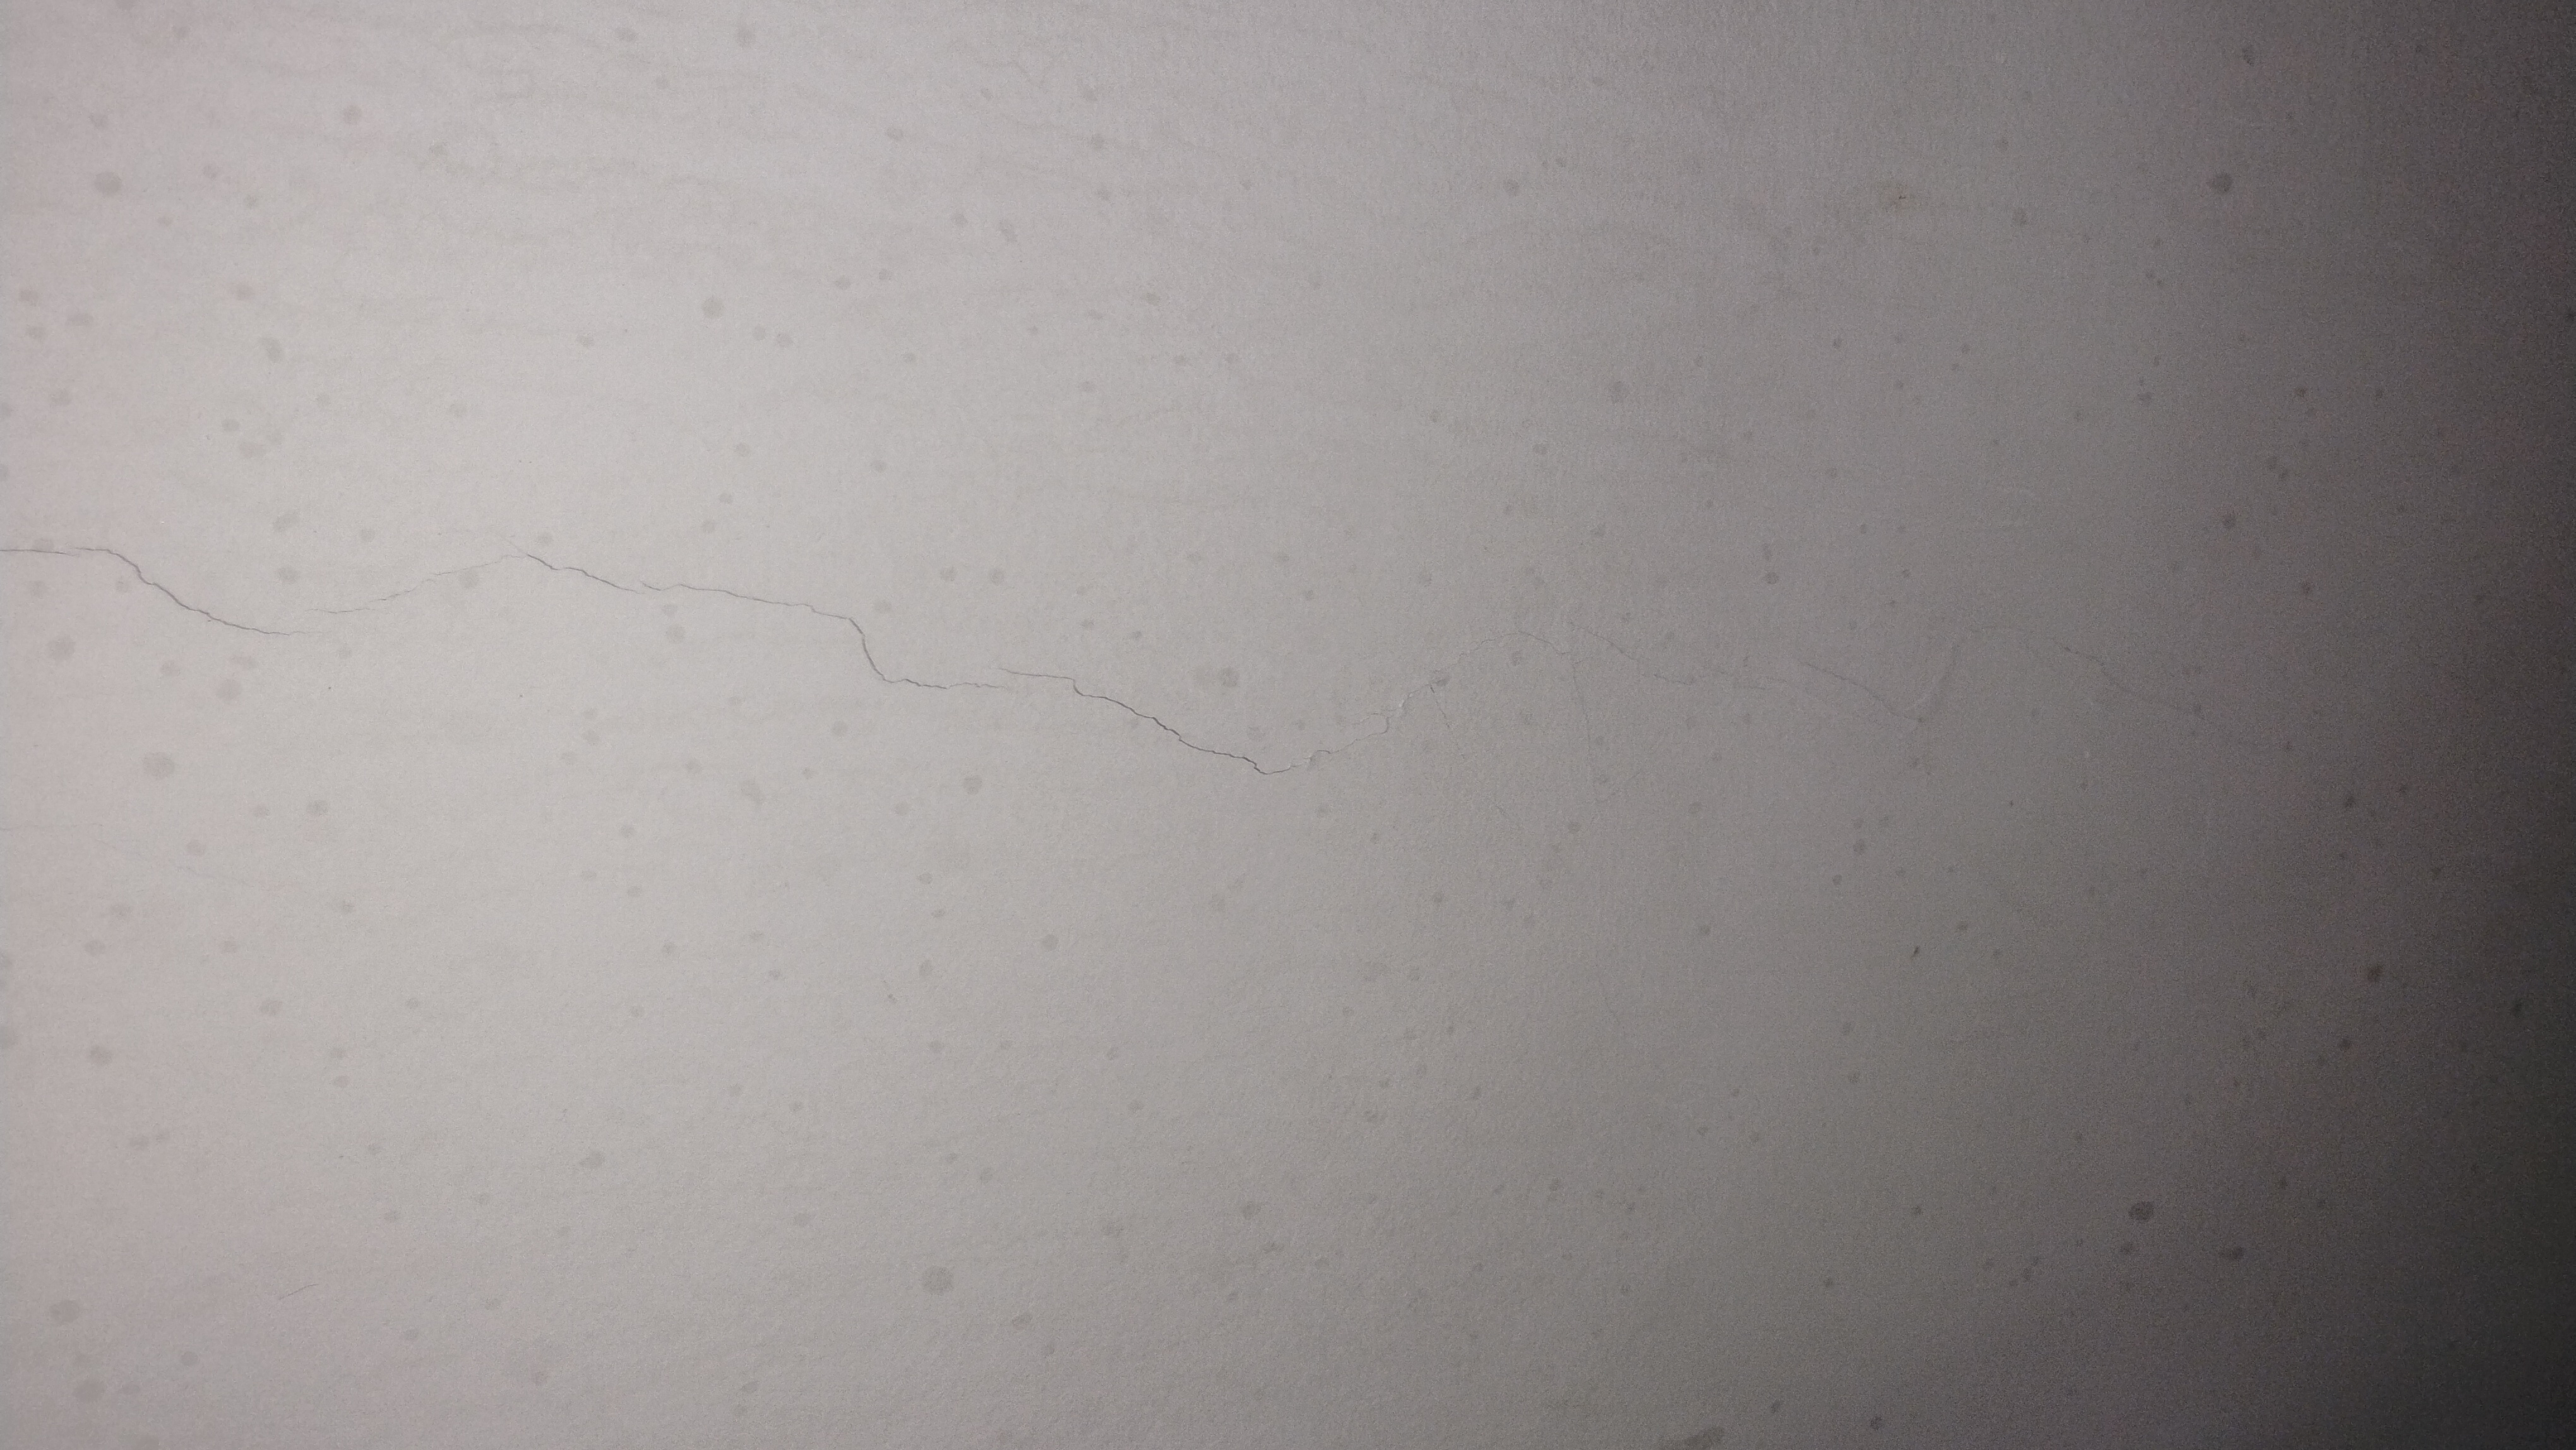
\includegraphics[width=\linewidth]{../img/IMG_20251109_151745353.jpg}\\[2pt]{\footnotesize\color{primary!60!black}Foto~64 -- 15:17:45}} \\[4pt]
\parbox{0.45\textwidth}{\centering
\includegraphics[width=\linewidth]{../img/IMG_20251109_151748443.jpg}\\[2pt]{\footnotesize\color{primary!60!black}Foto~65 -- 15:17:48}} & \parbox{0.45\textwidth}{\centering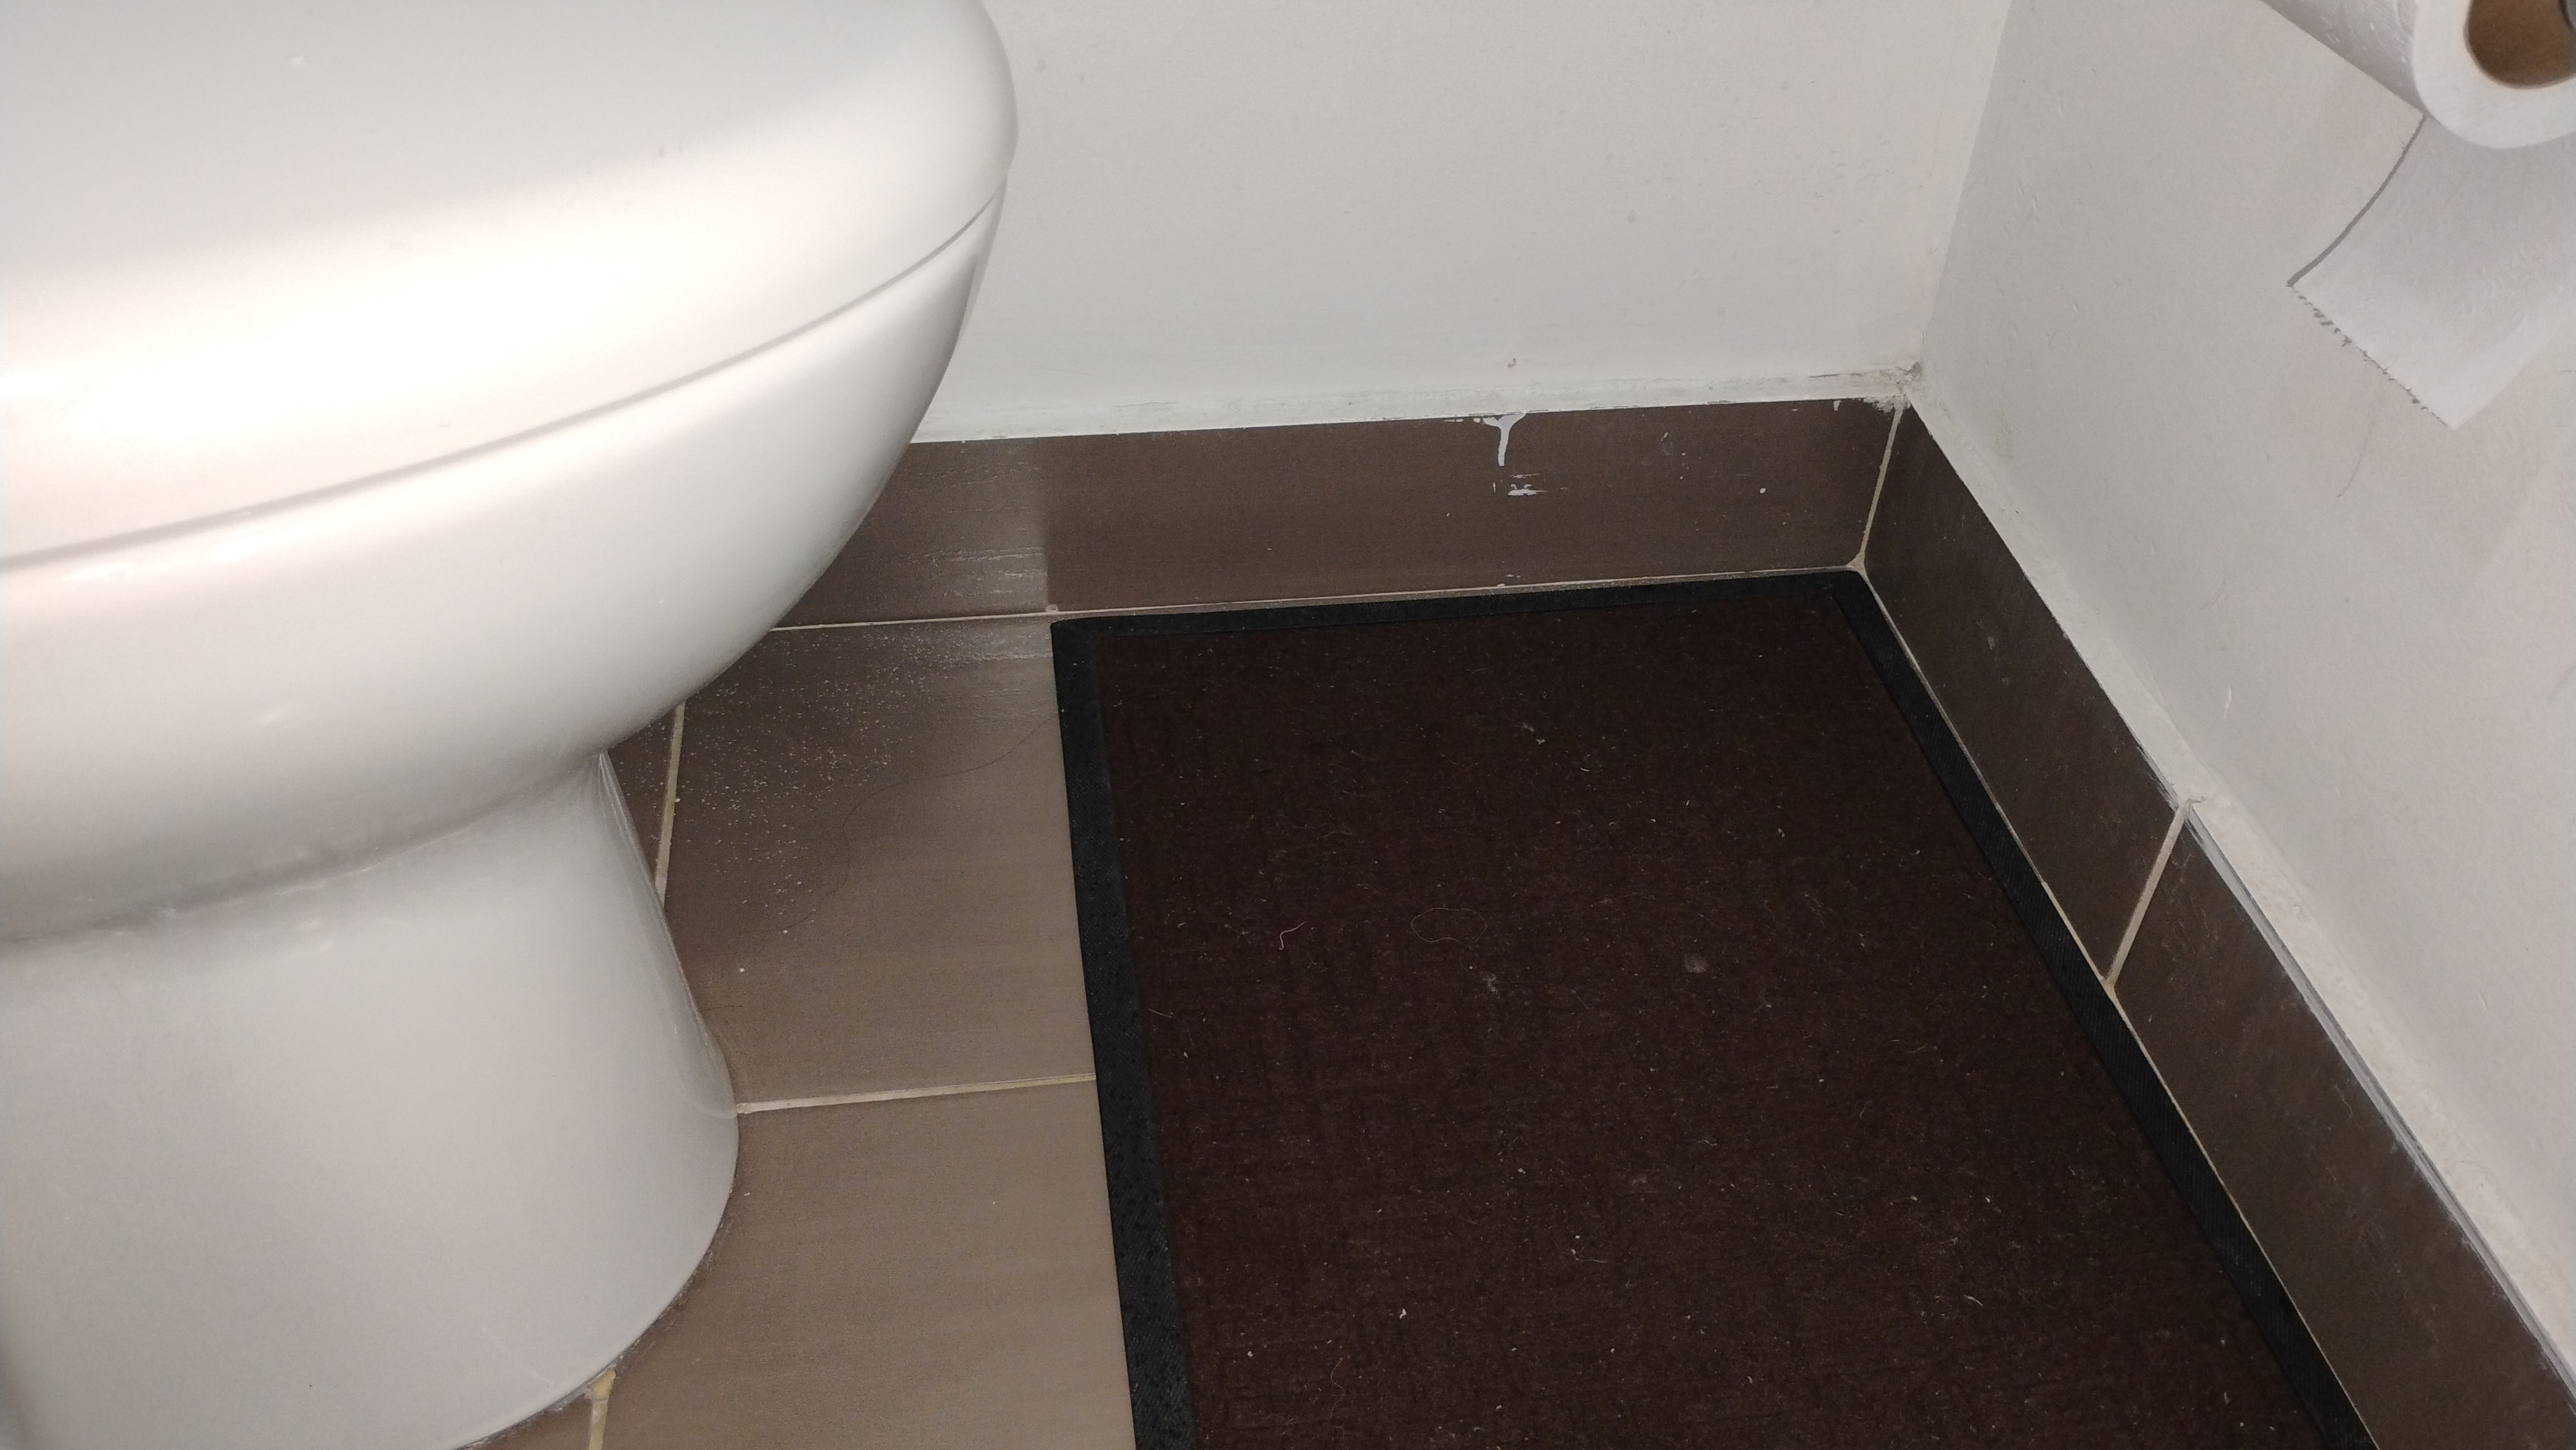
\includegraphics[width=\linewidth]{../img/IMG_20251109_151807312.jpg}\\[2pt]{\footnotesize\color{primary!60!black}Foto~66 -- 15:18:07}} \\[4pt]
\end{tabular}
\caption{Instalaciones Hidrosanitarias — Grifería, Válvulas y Tubería: Fotos 61 al 66.}\end{figure}
\newpage
\section{Baño 3}
\noindent\textbf{Estado general:} MALO.
\medskip
\noindent\textbf{Patologías identificadas:}
\begin{itemize}[leftmargin=*,nosep]
  \item \textbf{Filtración activa} en la unión muro-piso de la ducha — el agua de escorrentía ha penetrado por las boquillas desprendidas, generando desprendimiento del enchape en un área de 40 $\times$ 60 cm con pérdida total de adherencia.
  \item \textbf{Colonización fúngica extensa} en la totalidad de las juntas de la ducha — hongos negros y verdosos en las boquillas, con penetración al sustrato y olor a humedad característico.
  \item \textbf{Enchape abombado} en el muro de la ducha — se detecta sonido a hueco en un 70\% de la superficie, indicativo de pérdida de adherencia generalizada por saturación de humedad.
  \item \textbf{Corrosión avanzada} en la válvula mezcladora de la ducha y tubería de PVC expuesta — degradación del PVC por temperatura con manchas de sarro en las uniones y fugas en los empaques de la válvula.
  \item \textbf{Sanitario fisurado} en la base del inodoro — fisura horizontal en la porcelana de aproximadamente 5 cm, probablemente causada por golpe o asentamiento diferencial.
  \item \textbf{Grifería del lavamanos} con corrosión generalizada y pérdida de estanqueidad — goteo constante que ha generado una mancha de óxido en el mesón y acumulación de sarro en la base del caño.
  \item \textbf{Desprendimiento de pañete} en el cielorraso con deformación del perfil de drywall — indicativo de filtración recurrente desde el nivel superior con saturación del panel de yeso.
  \item \textbf{Pérdida de pendiente} en el piso de la ducha — se observa acumulación de agua en la esquina noroccidental por deficiente evacuación, con encharcamiento permanente y degradación del acabado superficial.
\end{itemize}
\medskip
\noindent\textbf{Zonas críticas:} Ducha (filtración activa, hongos, enchape abombado), sanitario (fisurado), grifería lavamanos (goteo), cielorraso (pañete desprendido), piso de ducha (pendiente deficiente).
\bigskip
\begin{figure}[H]
\centering
\begin{tabular}{cc}
\parbox{0.45\textwidth}{\centering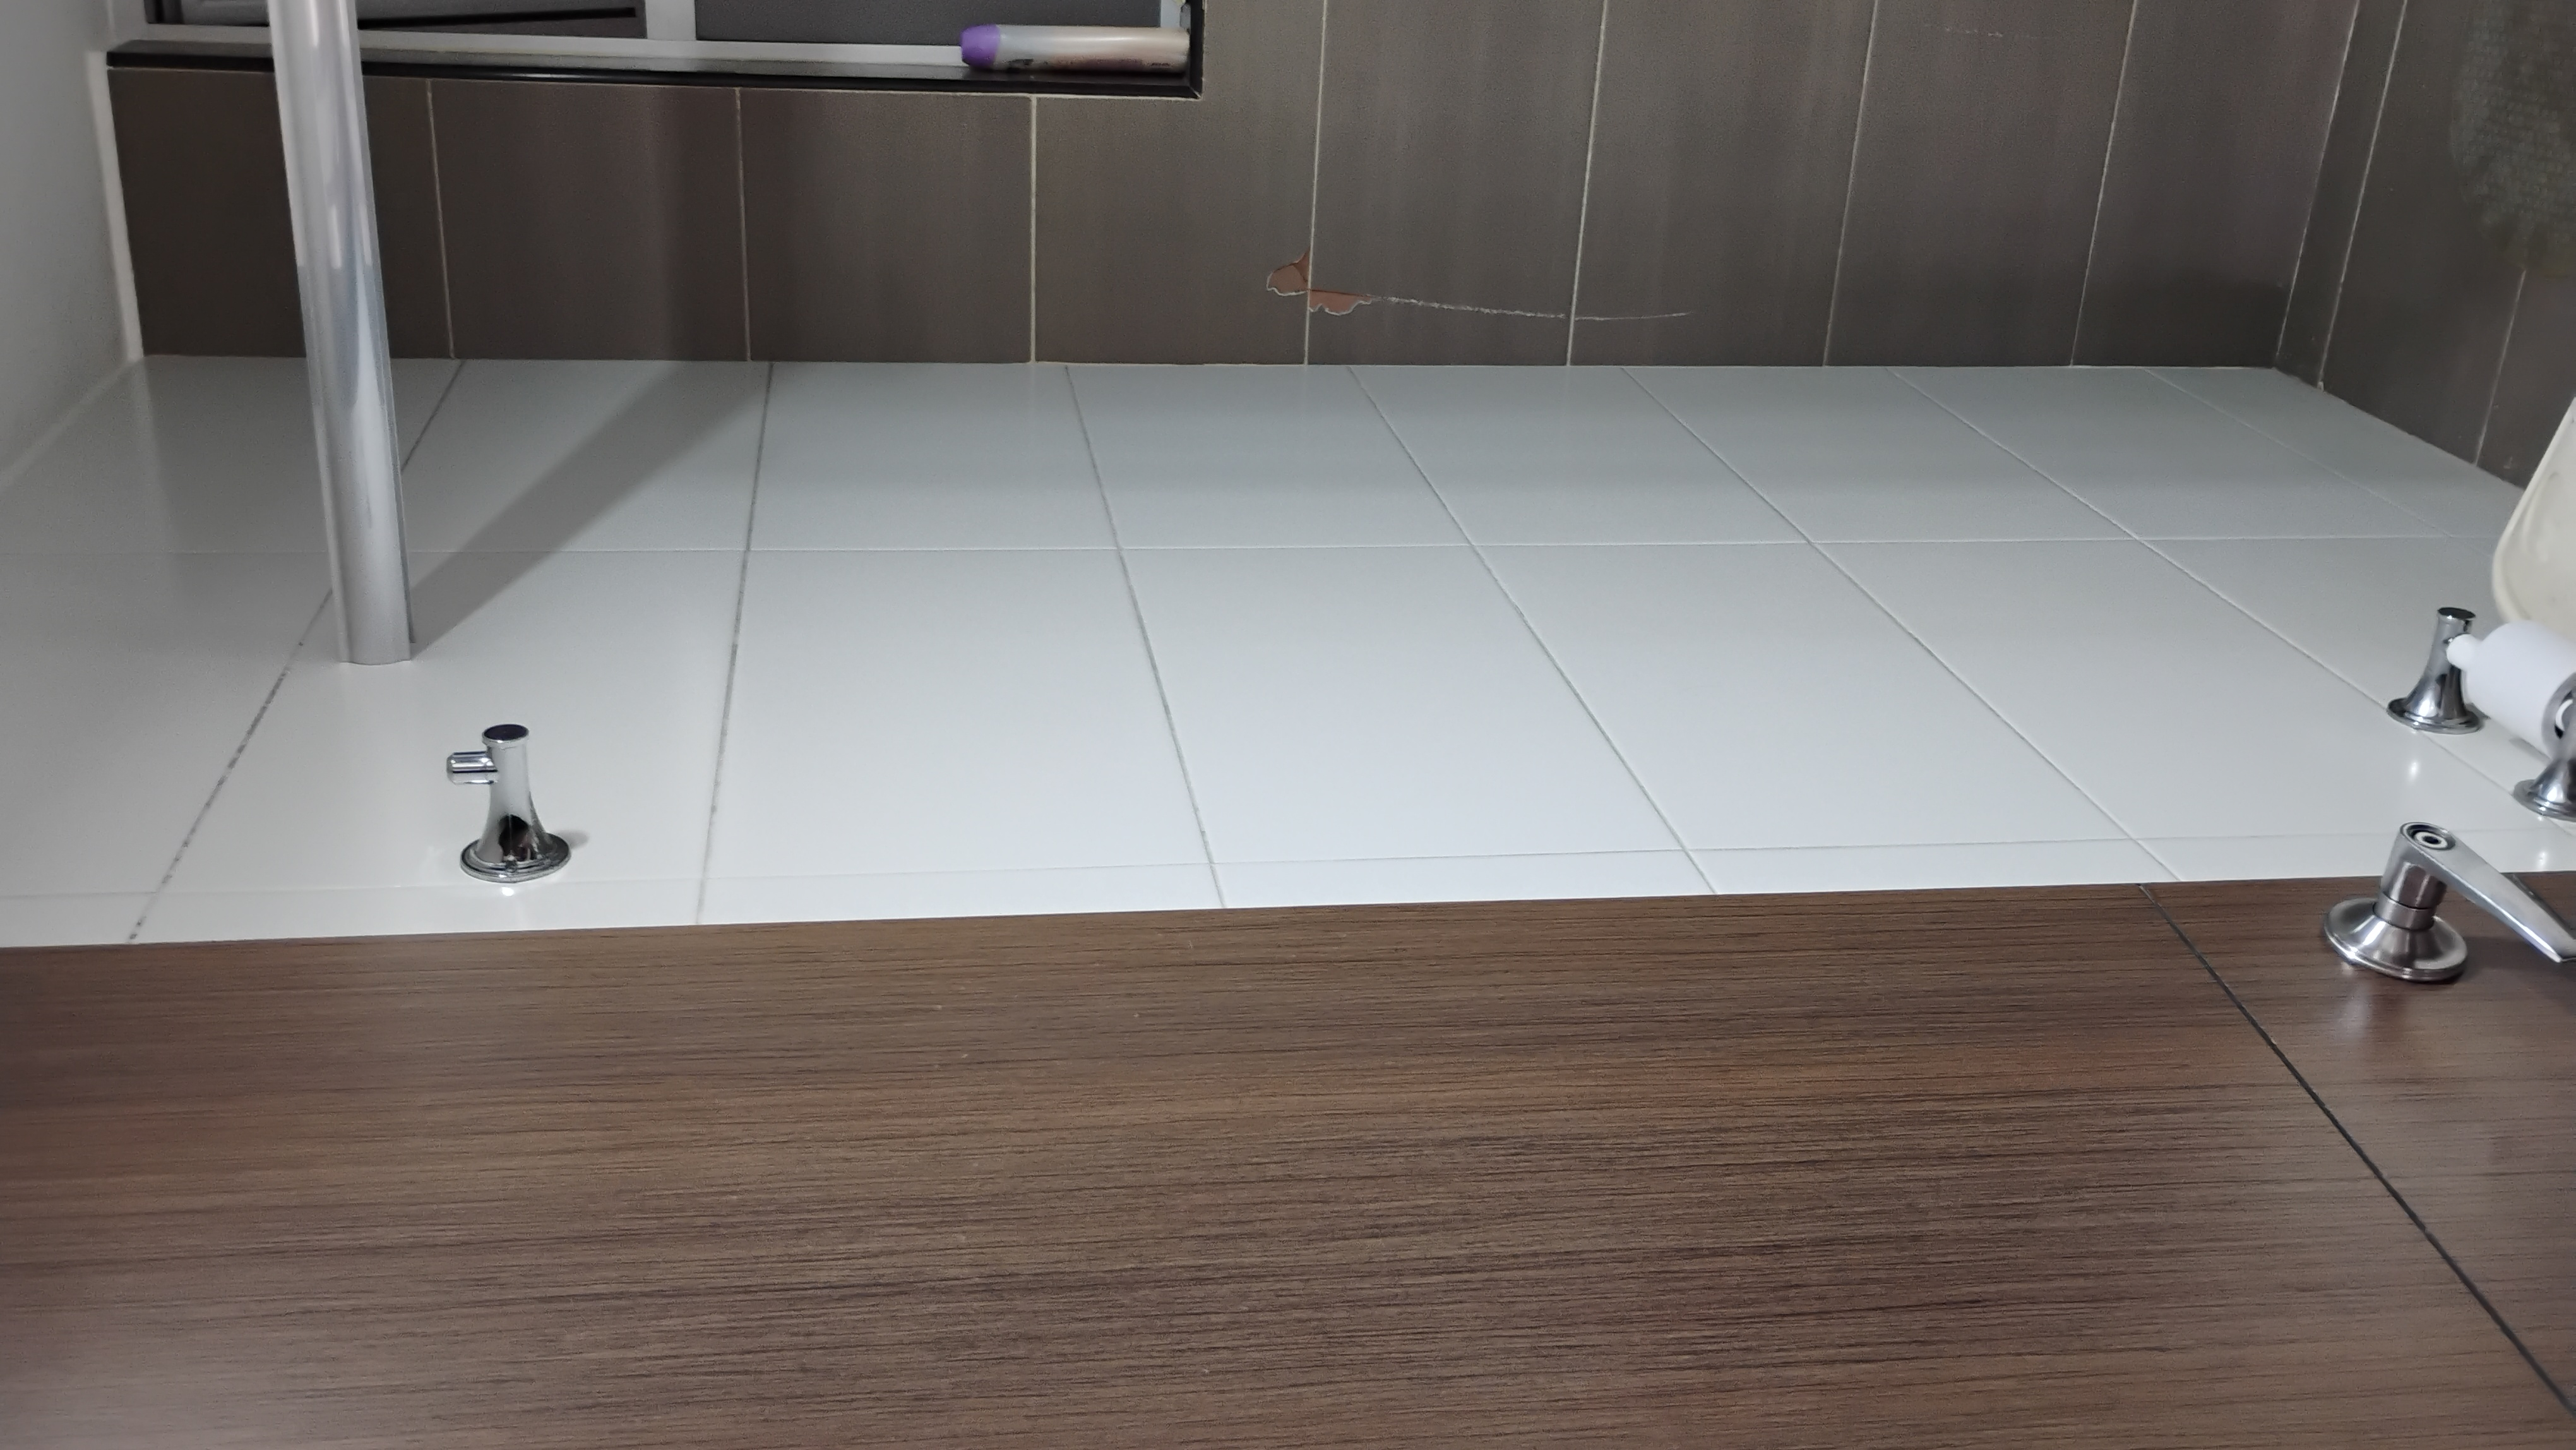
\includegraphics[width=\linewidth]{../img/IMG_20251109_150559222.jpg}\\[2pt]{\footnotesize\color{primary!60!black}Foto~67 -- 15:05:59}} & \parbox{0.45\textwidth}{\centering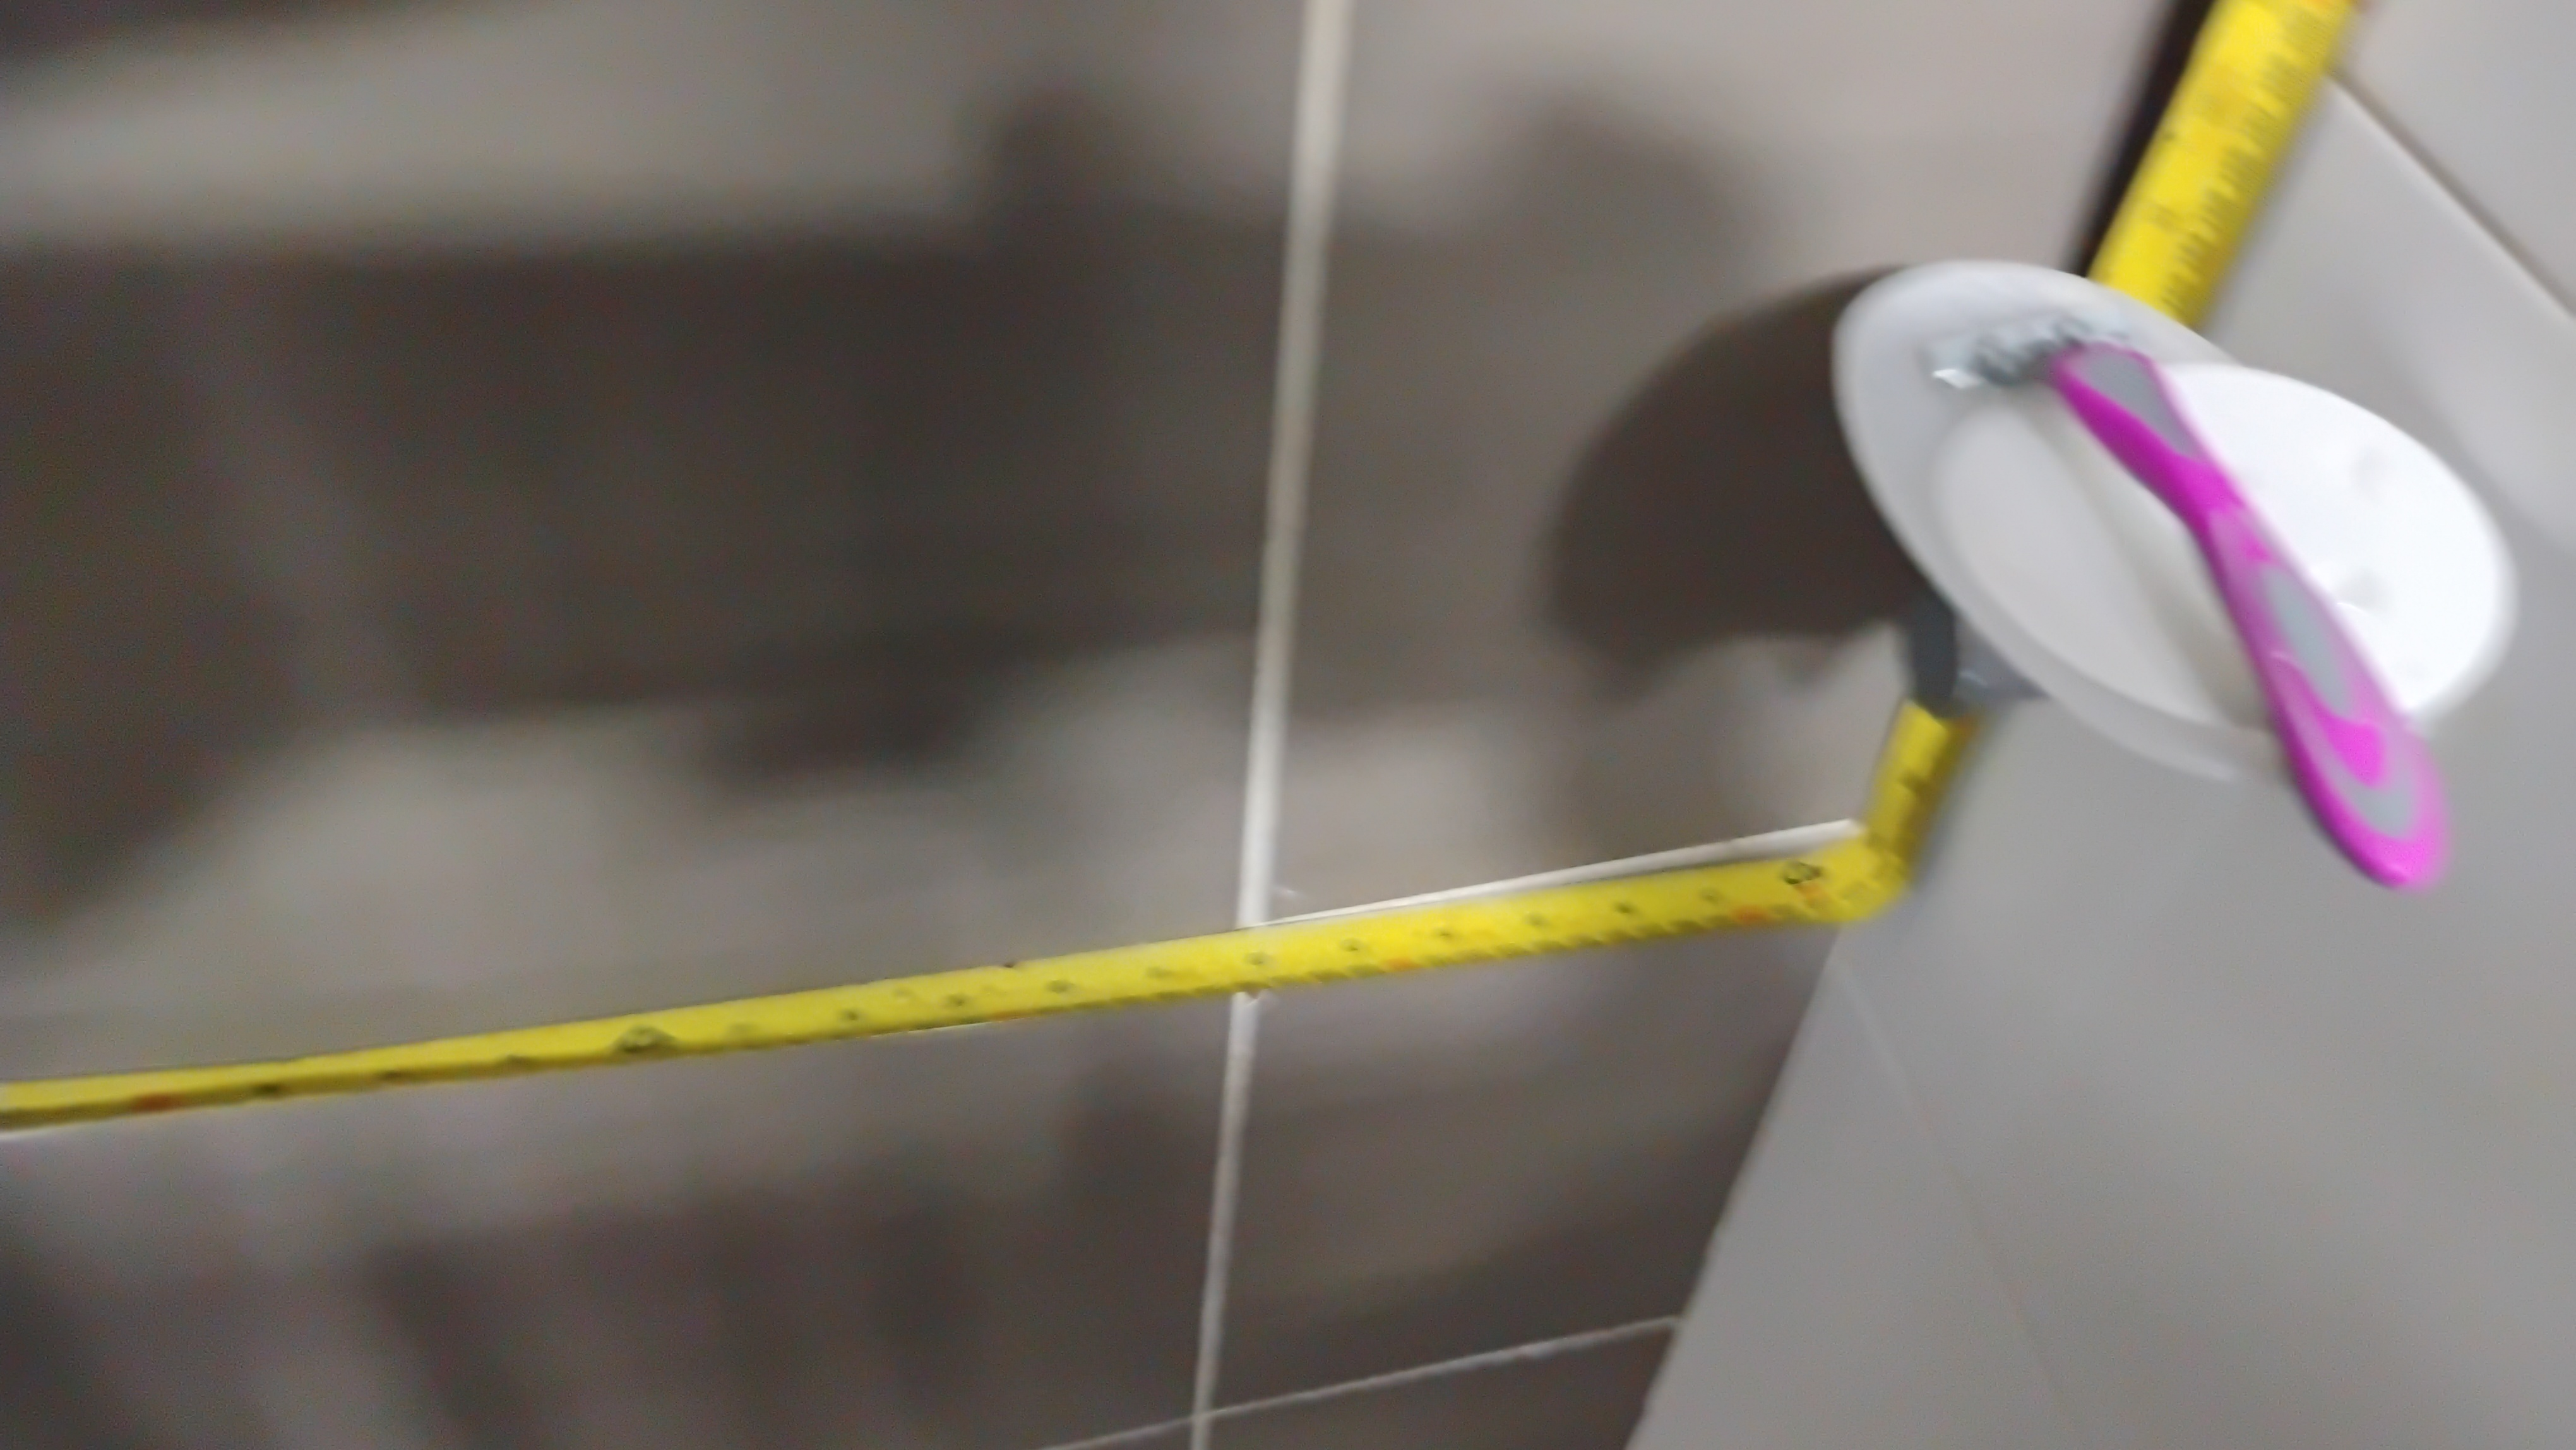
\includegraphics[width=\linewidth]{../img/IMG_20251109_150935585.jpg}\\[2pt]{\footnotesize\color{primary!60!black}Foto~68 -- 15:09:35}} \\[4pt]
\parbox{0.45\textwidth}{\centering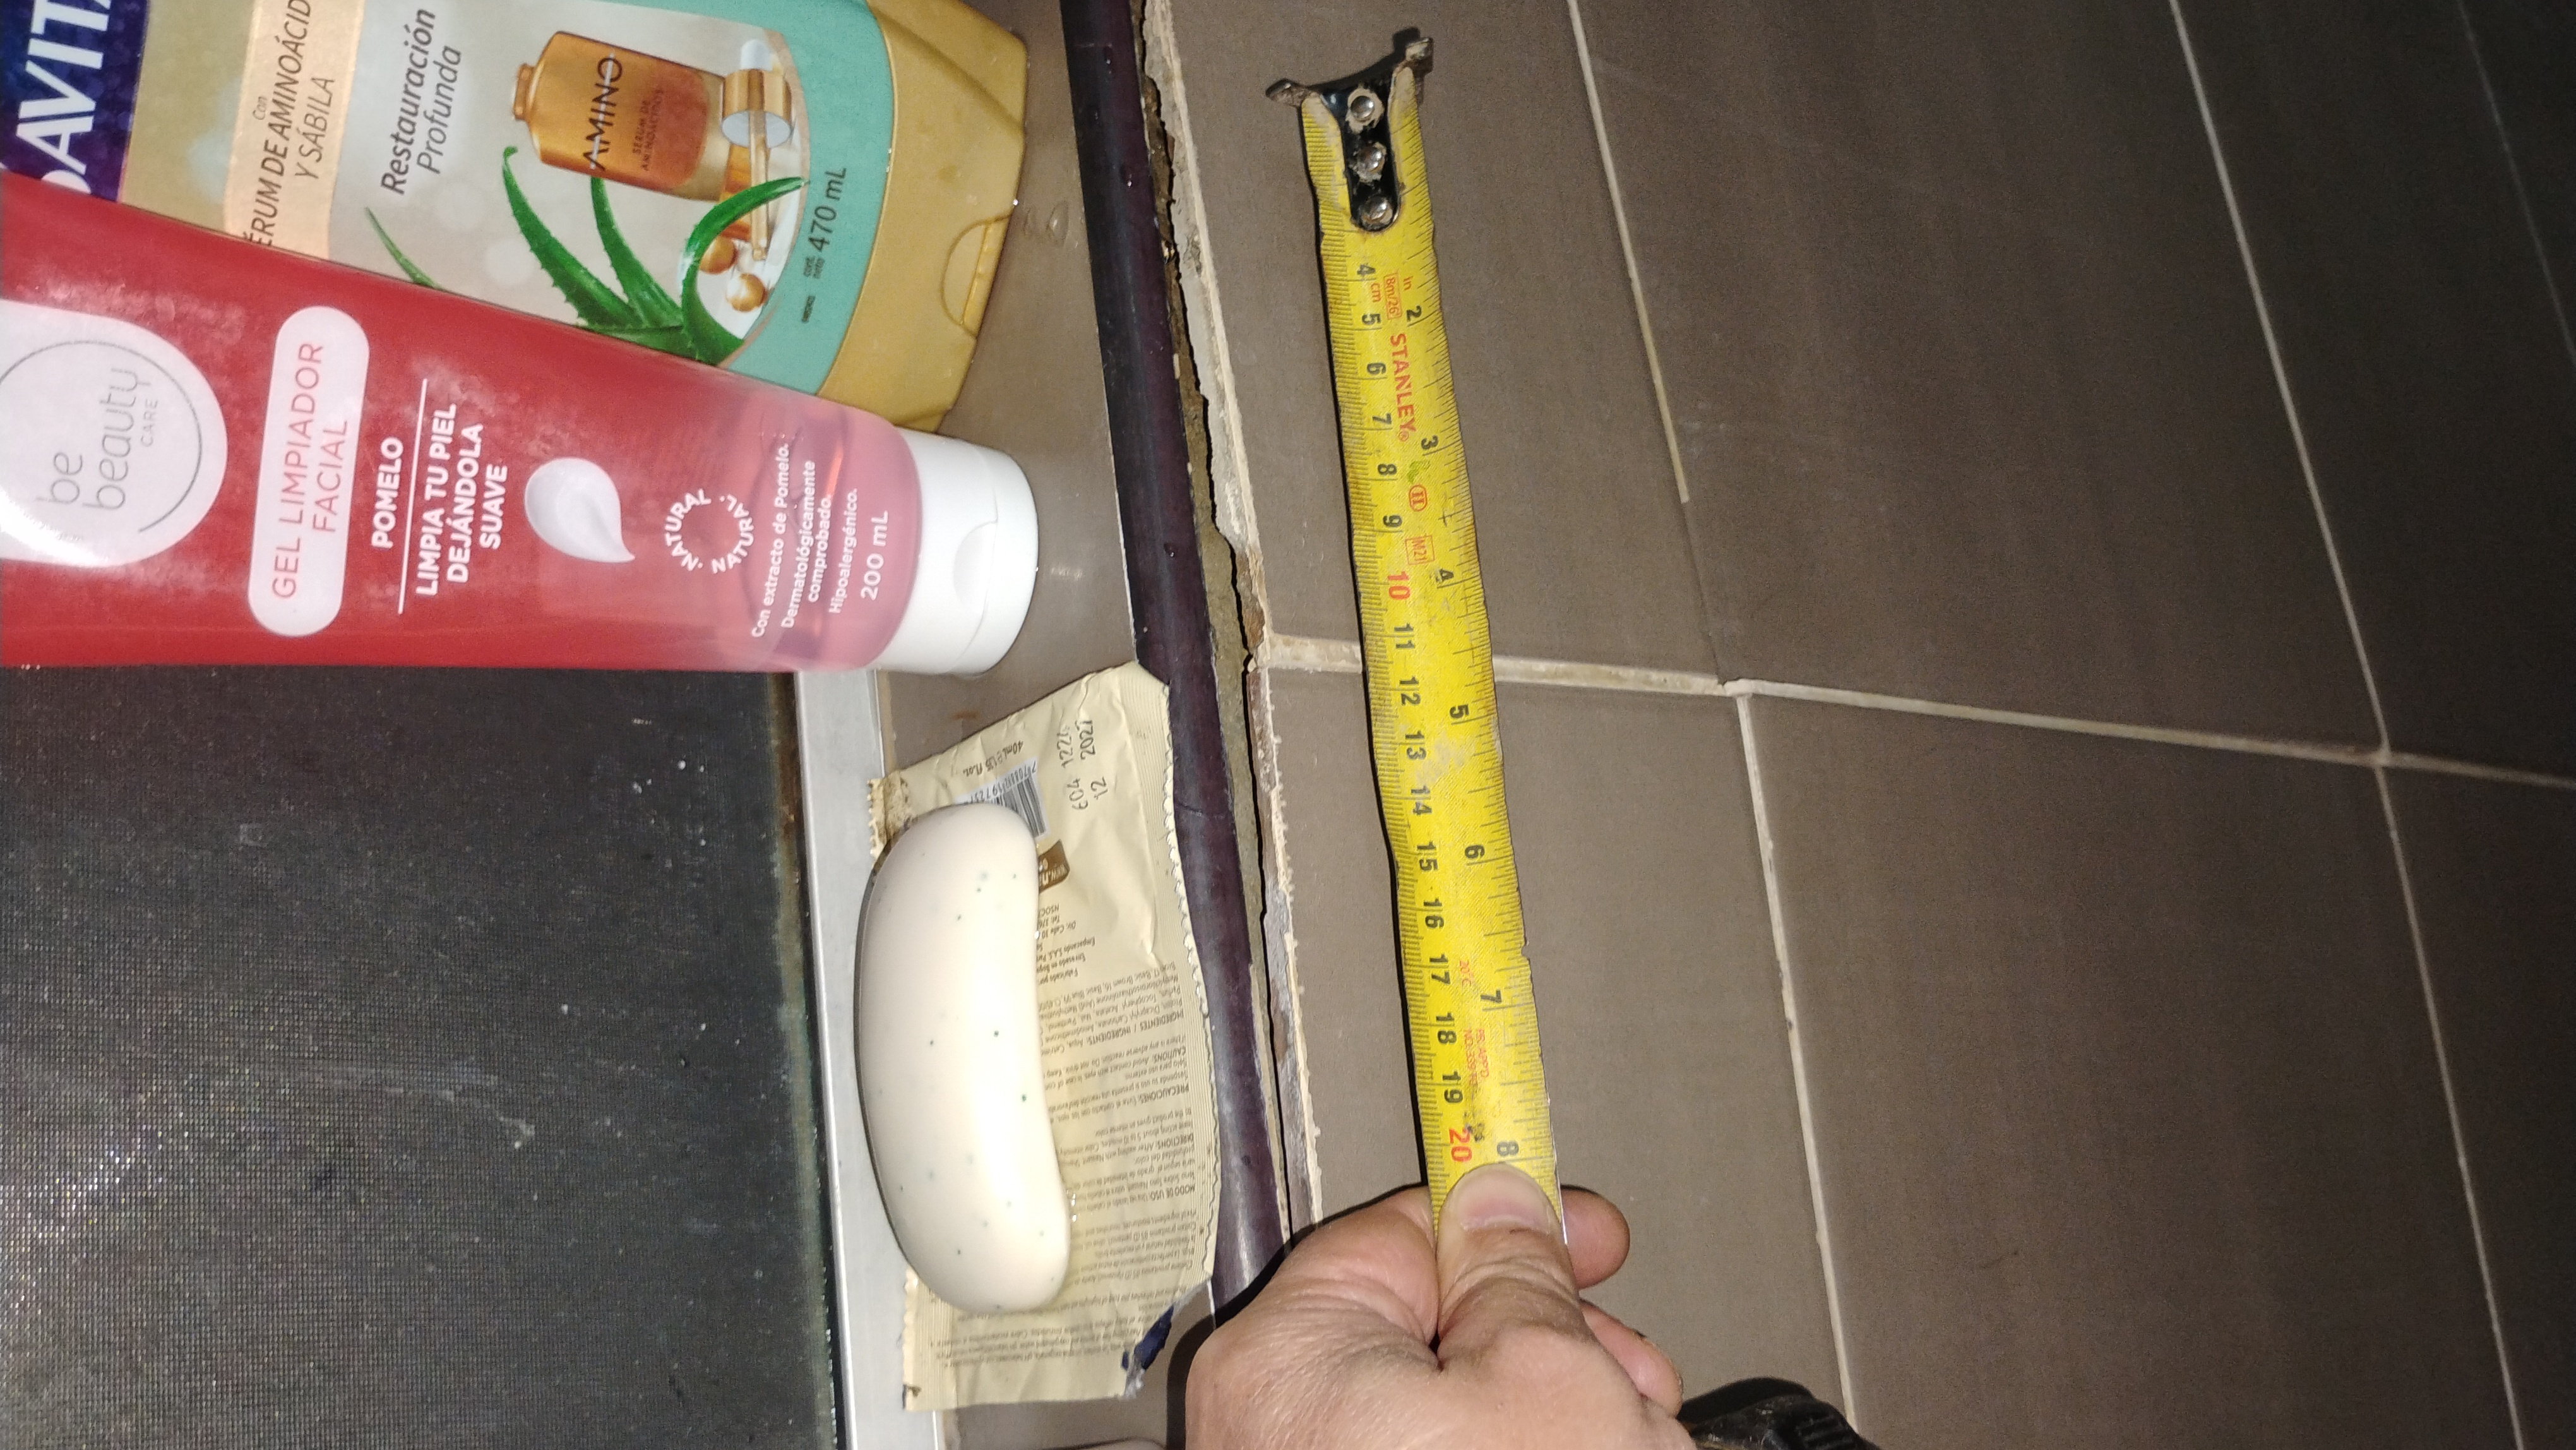
\includegraphics[width=\linewidth]{../img/IMG_20251109_151131173.jpg}\\[2pt]{\footnotesize\color{primary!60!black}Foto~69 -- 15:11:31}} & \parbox{0.45\textwidth}{\centering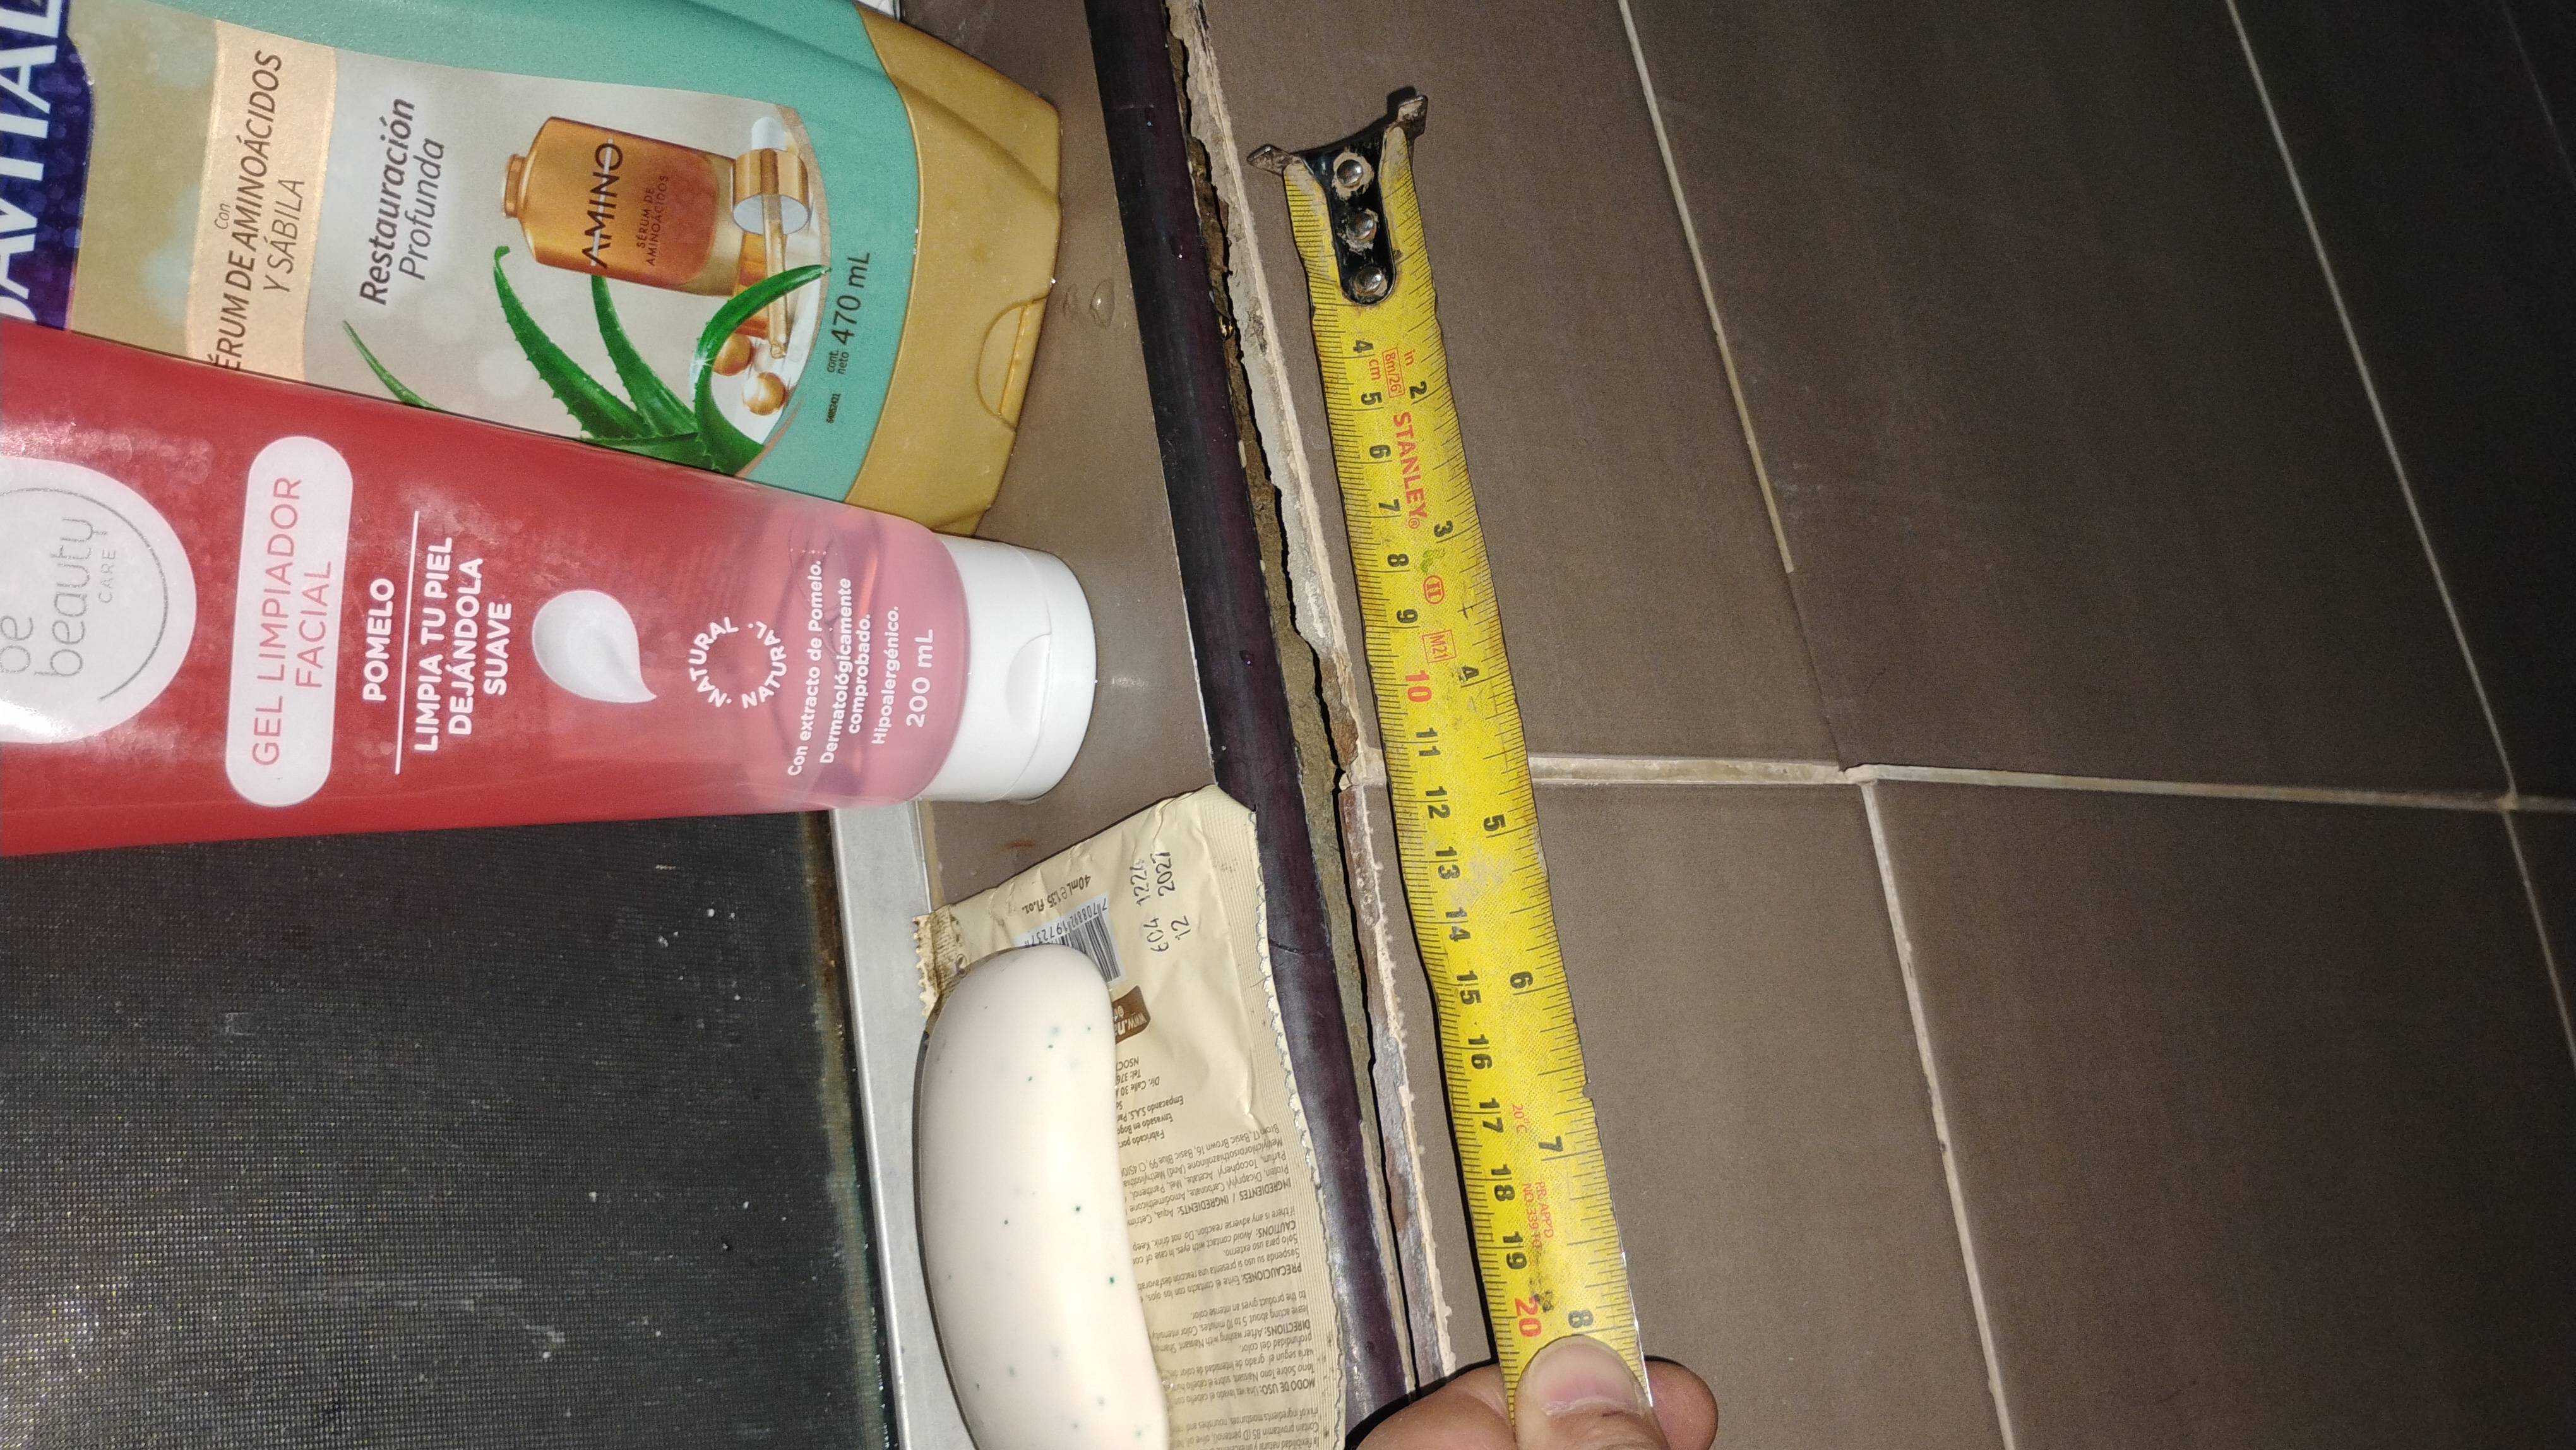
\includegraphics[width=\linewidth]{../img/IMG_20251109_151135245.jpg}\\[2pt]{\footnotesize\color{primary!60!black}Foto~70 -- 15:11:35}} \\[4pt]
\parbox{0.45\textwidth}{\centering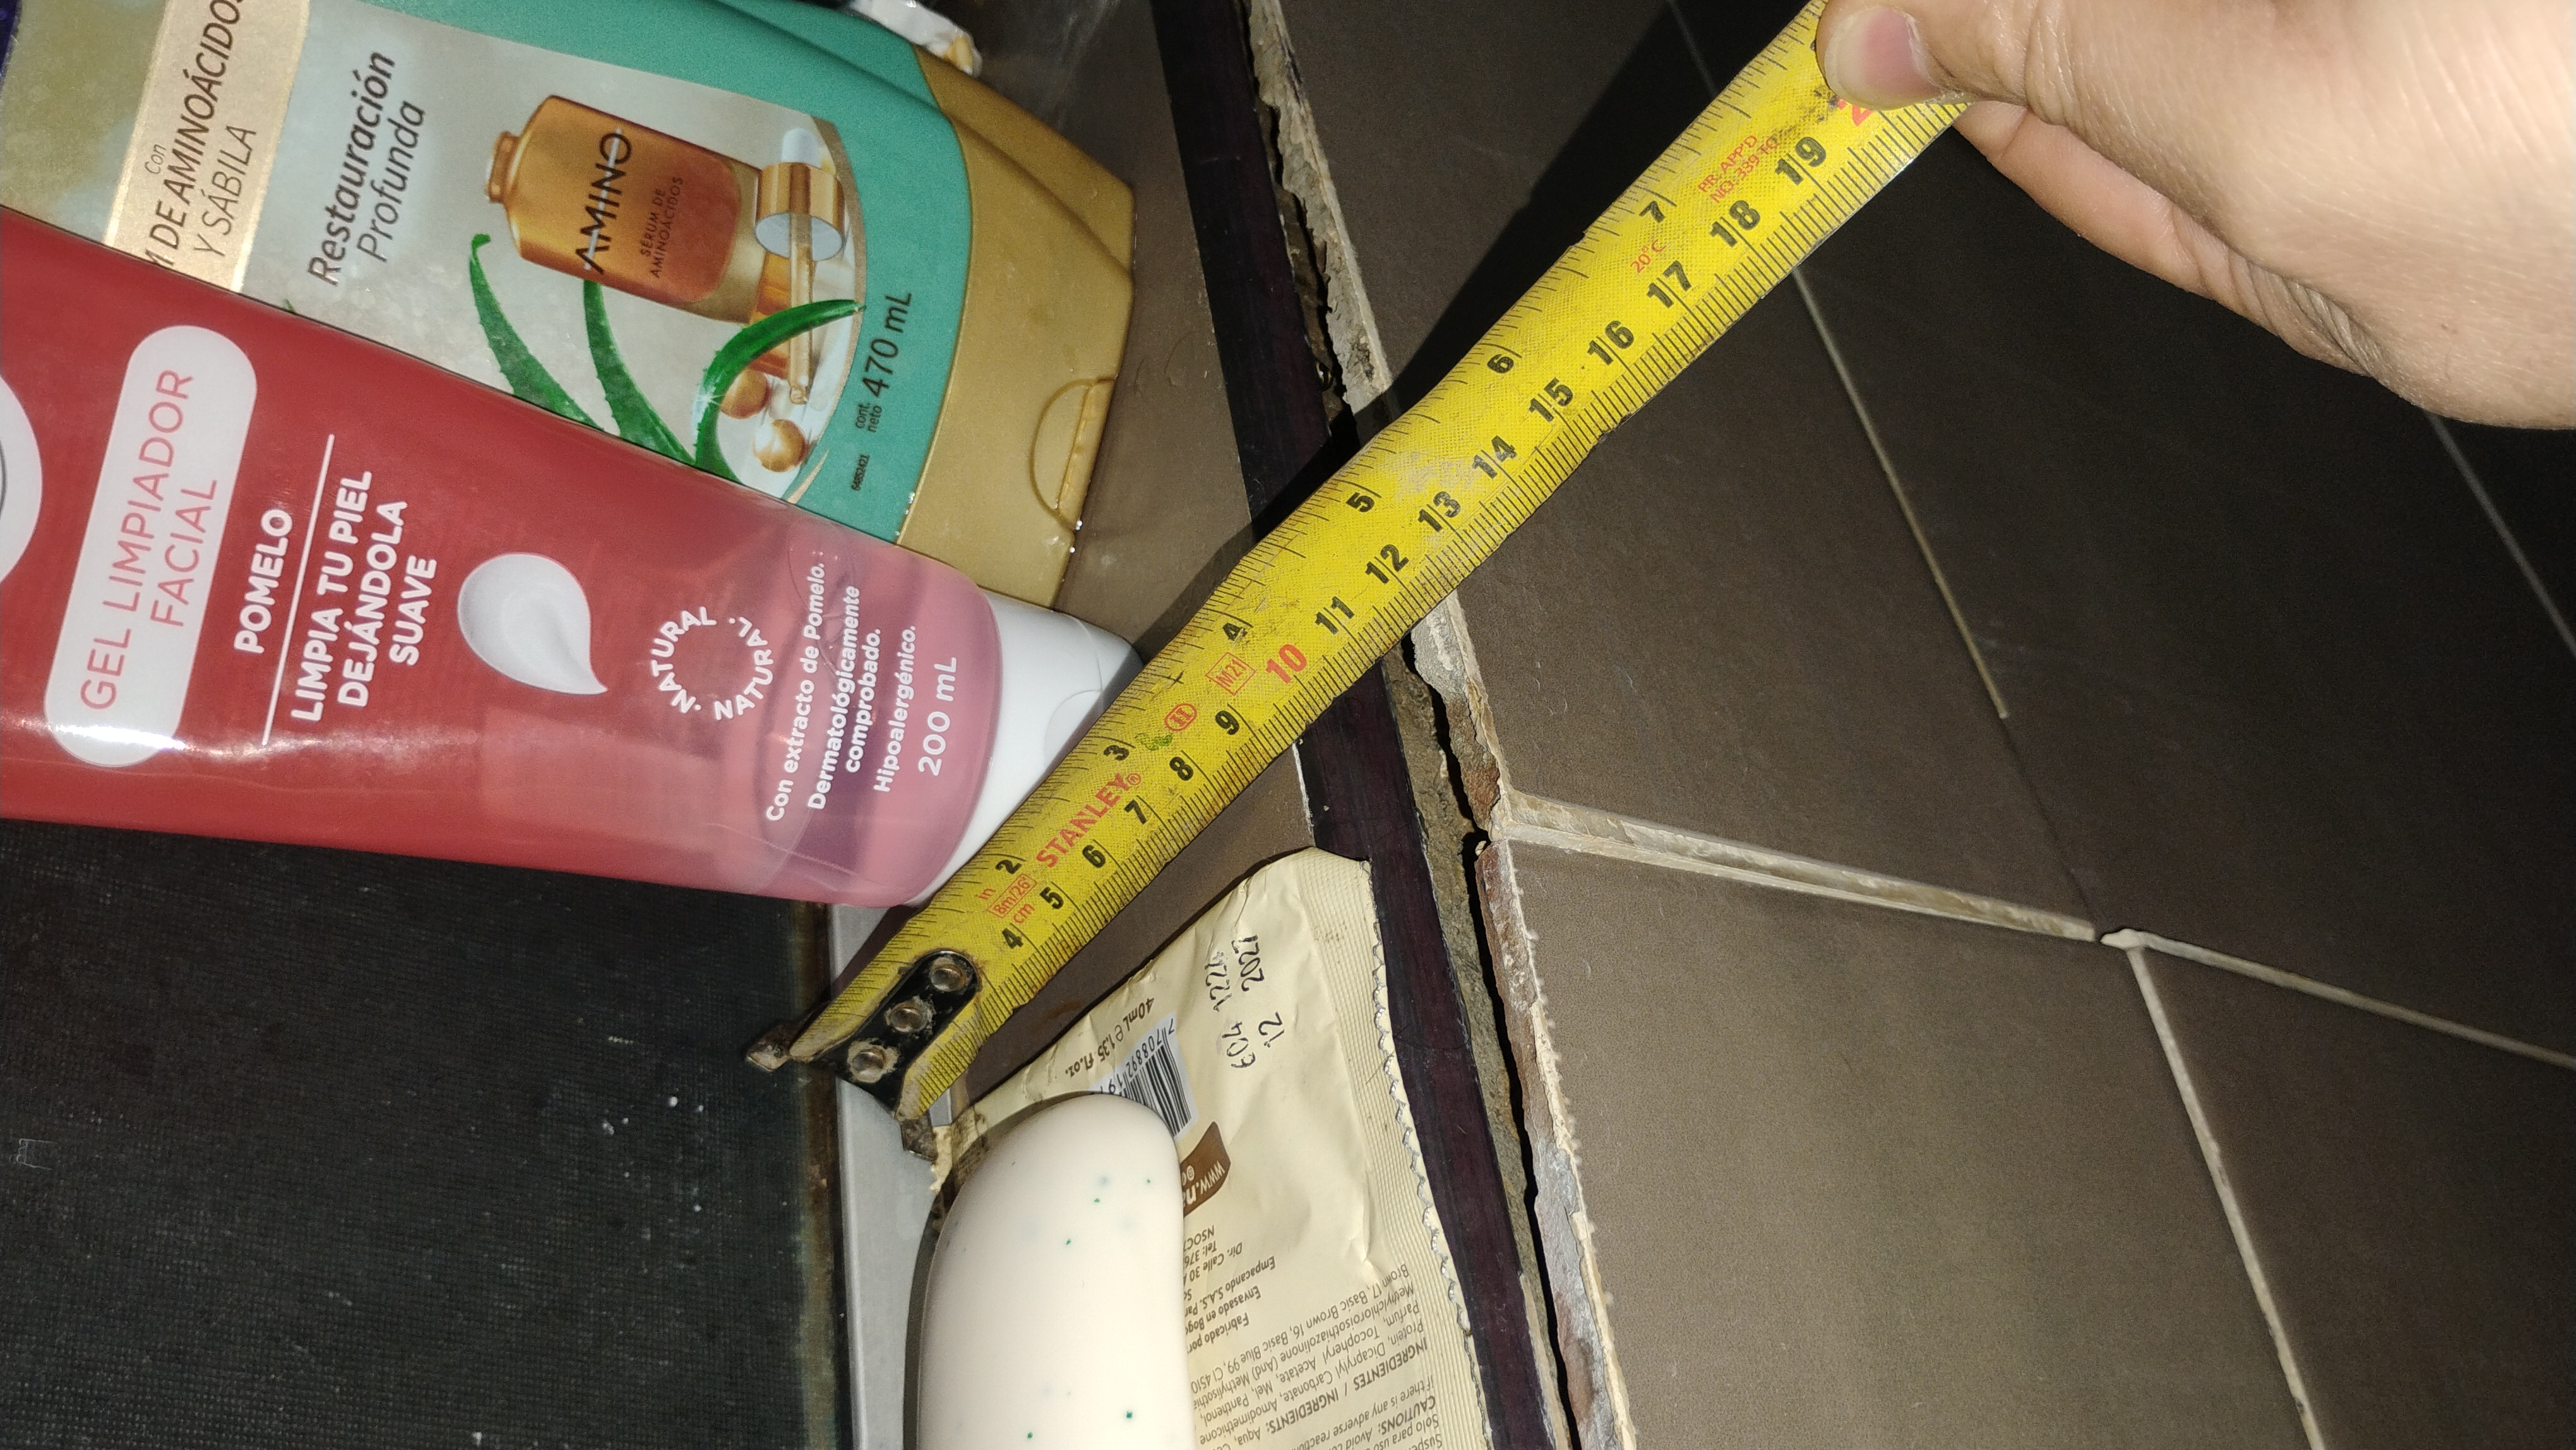
\includegraphics[width=\linewidth]{../img/IMG_20251109_151143423.jpg}\\[2pt]{\footnotesize\color{primary!60!black}Foto~71 -- 15:11:43}} & \parbox{0.45\textwidth}{\centering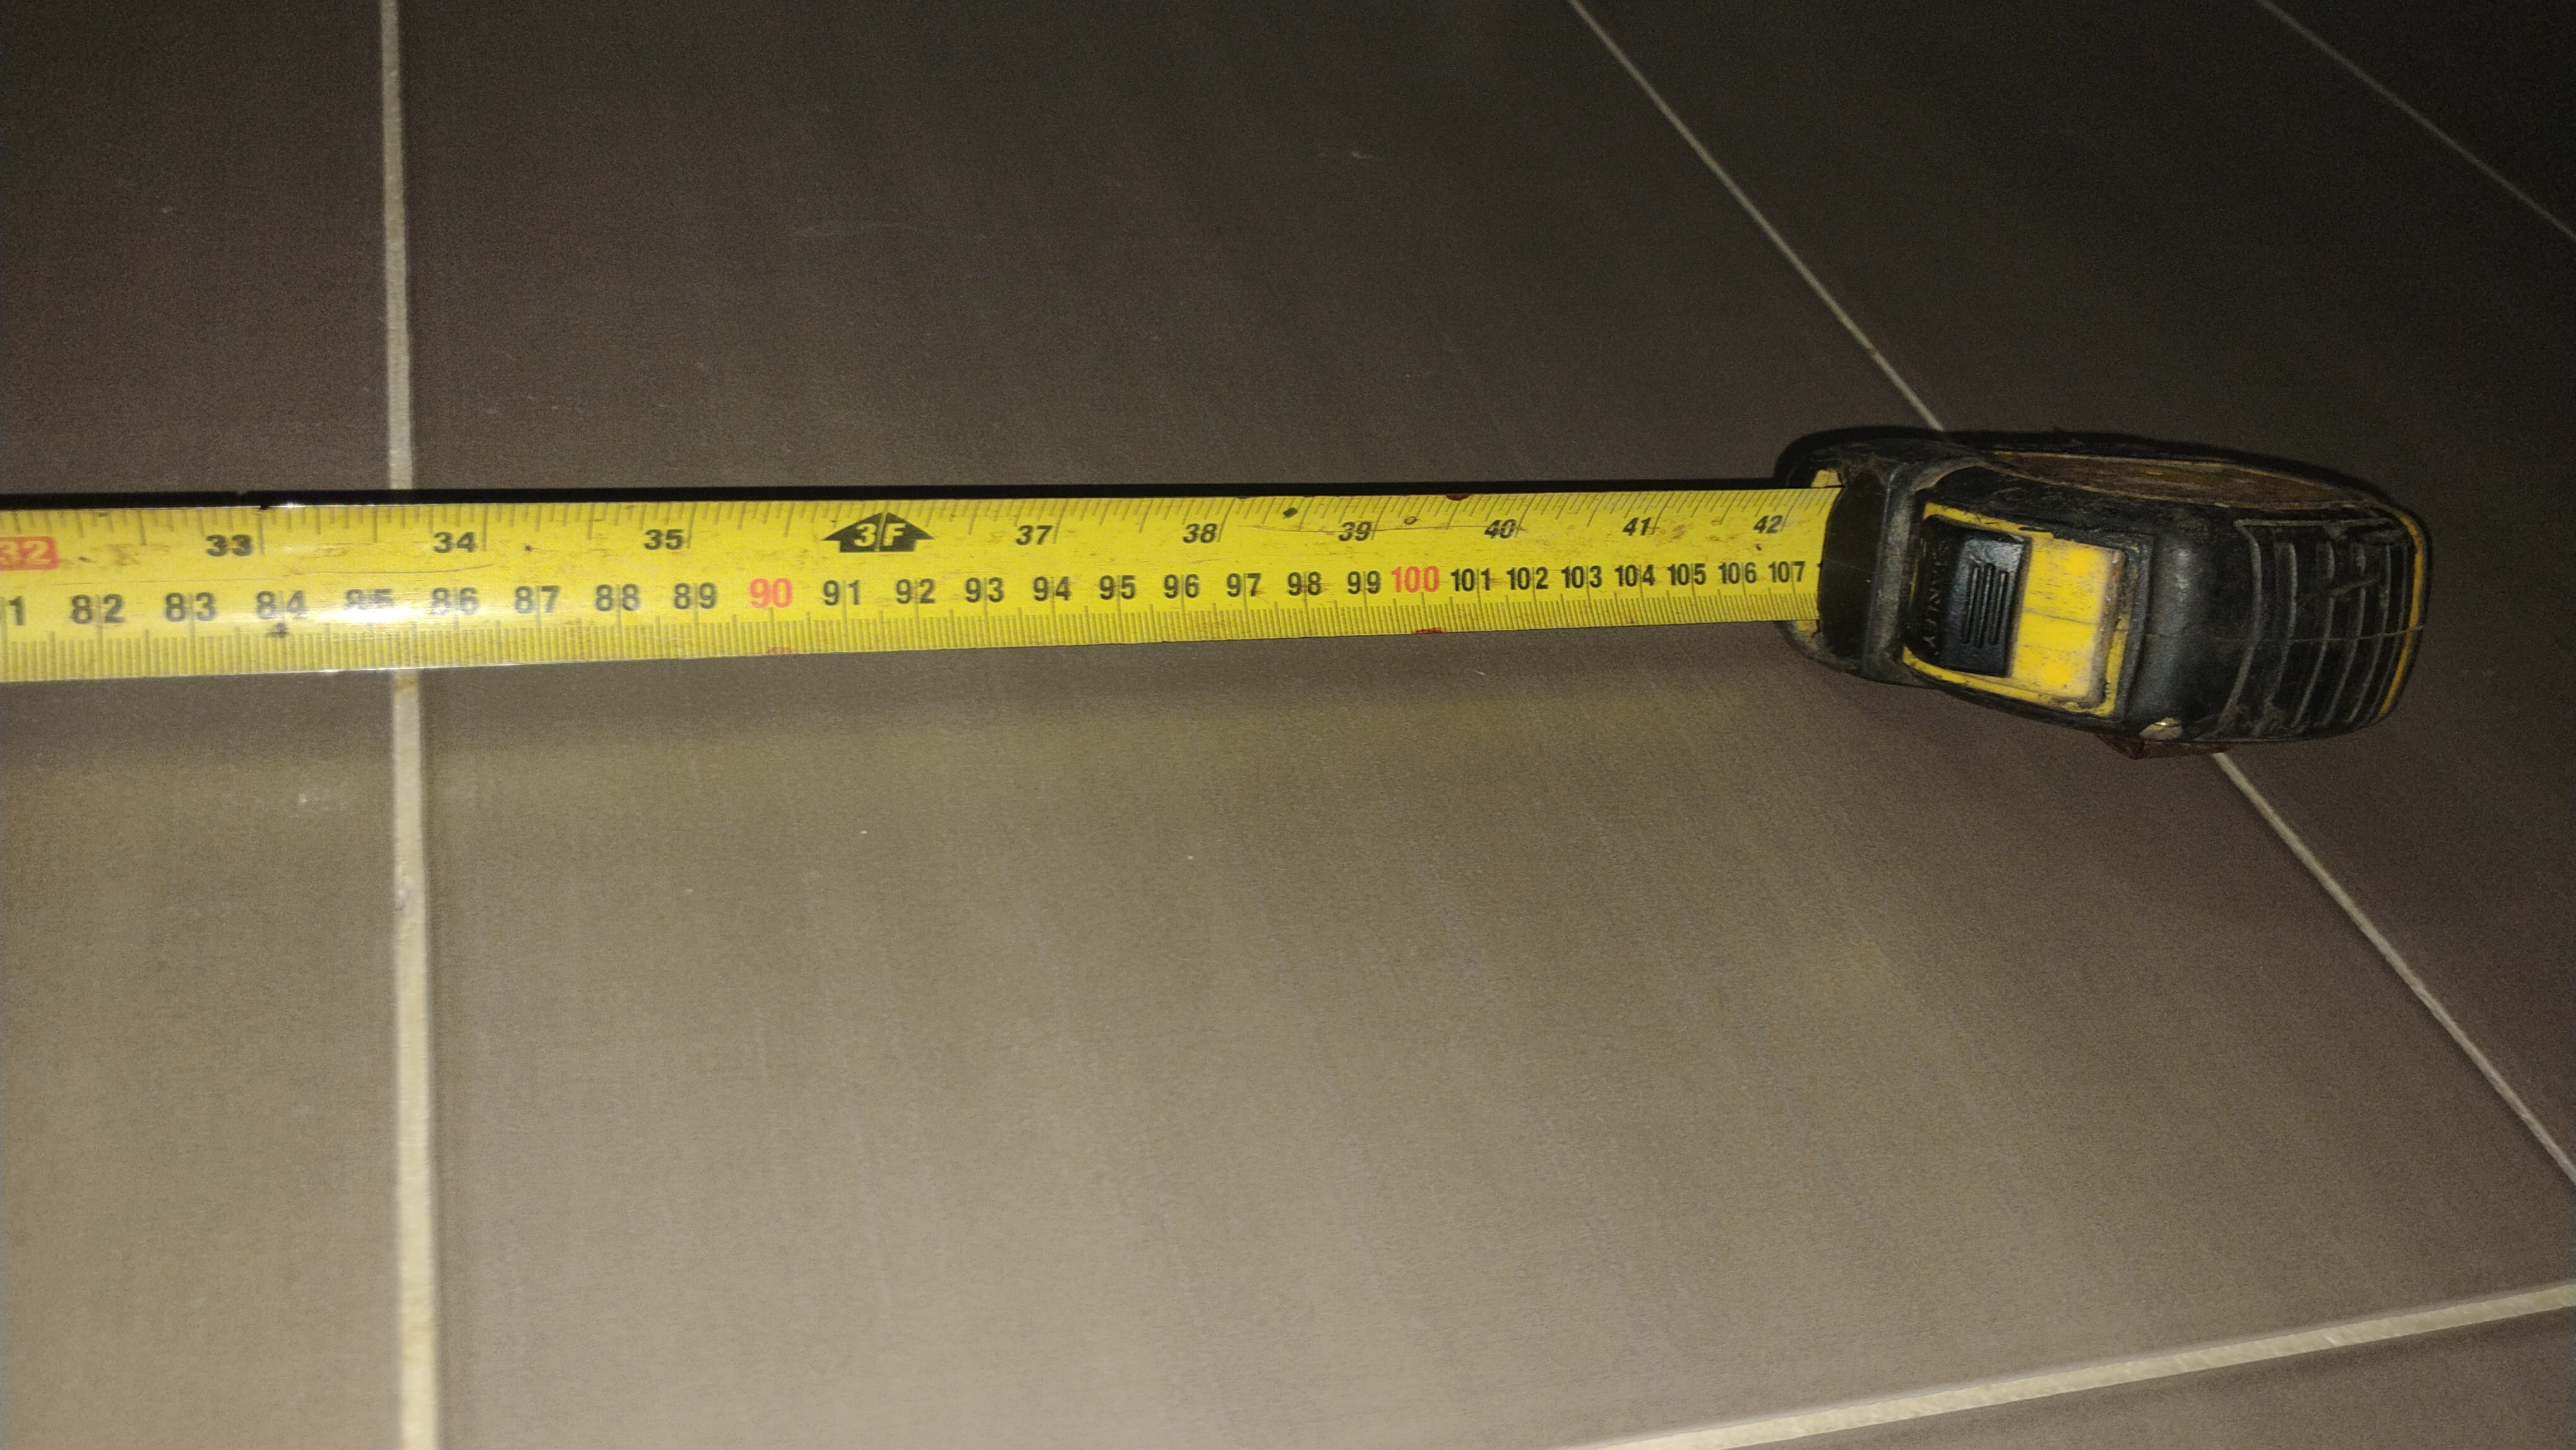
\includegraphics[width=\linewidth]{../img/IMG_20251109_151322318.jpg}\\[2pt]{\footnotesize\color{primary!60!black}Foto~72 -- 15:13:22}} \\[4pt]
\end{tabular}
\caption{Zona de Ducha — Filtración Activa y Colonización Fúngica: Fotos 67 al 72.}\end{figure}
\newpage
\begin{figure}[H]
\centering
\begin{tabular}{cc}
\parbox{0.45\textwidth}{\centering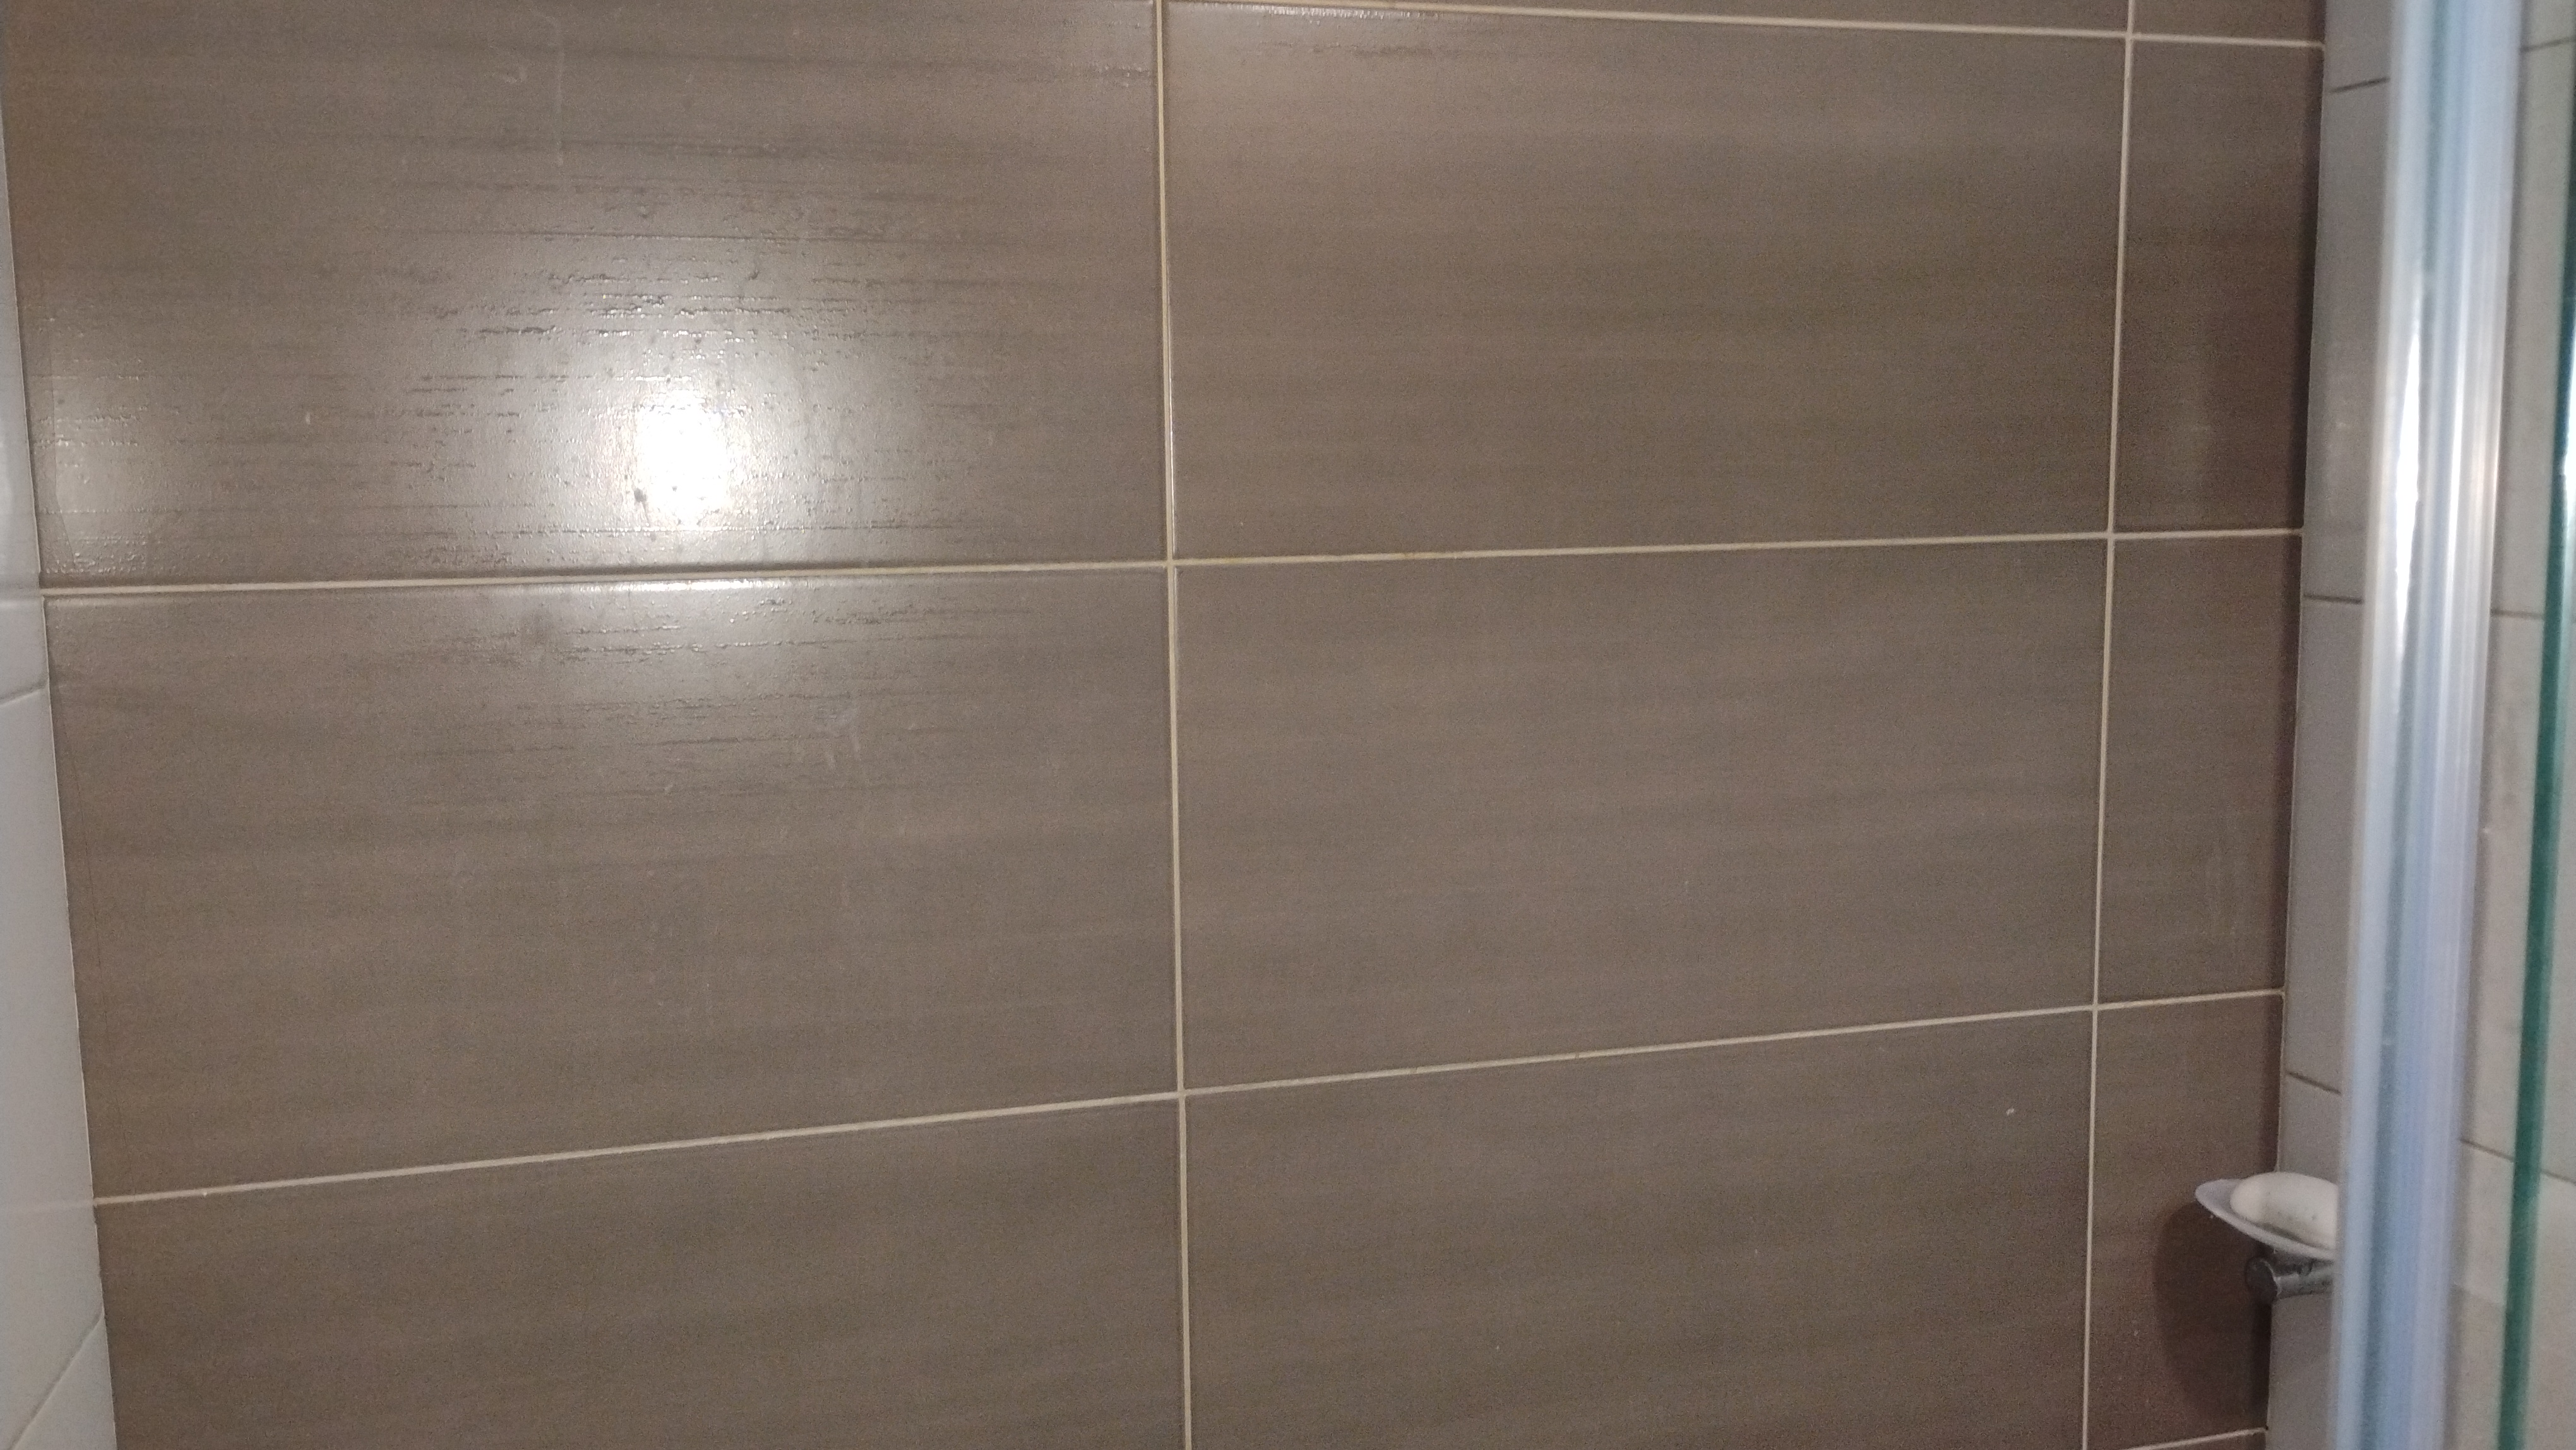
\includegraphics[width=\linewidth]{../img/IMG_20251109_151437315.jpg}\\[2pt]{\footnotesize\color{primary!60!black}Foto~73 -- 15:14:37}} & \parbox{0.45\textwidth}{\centering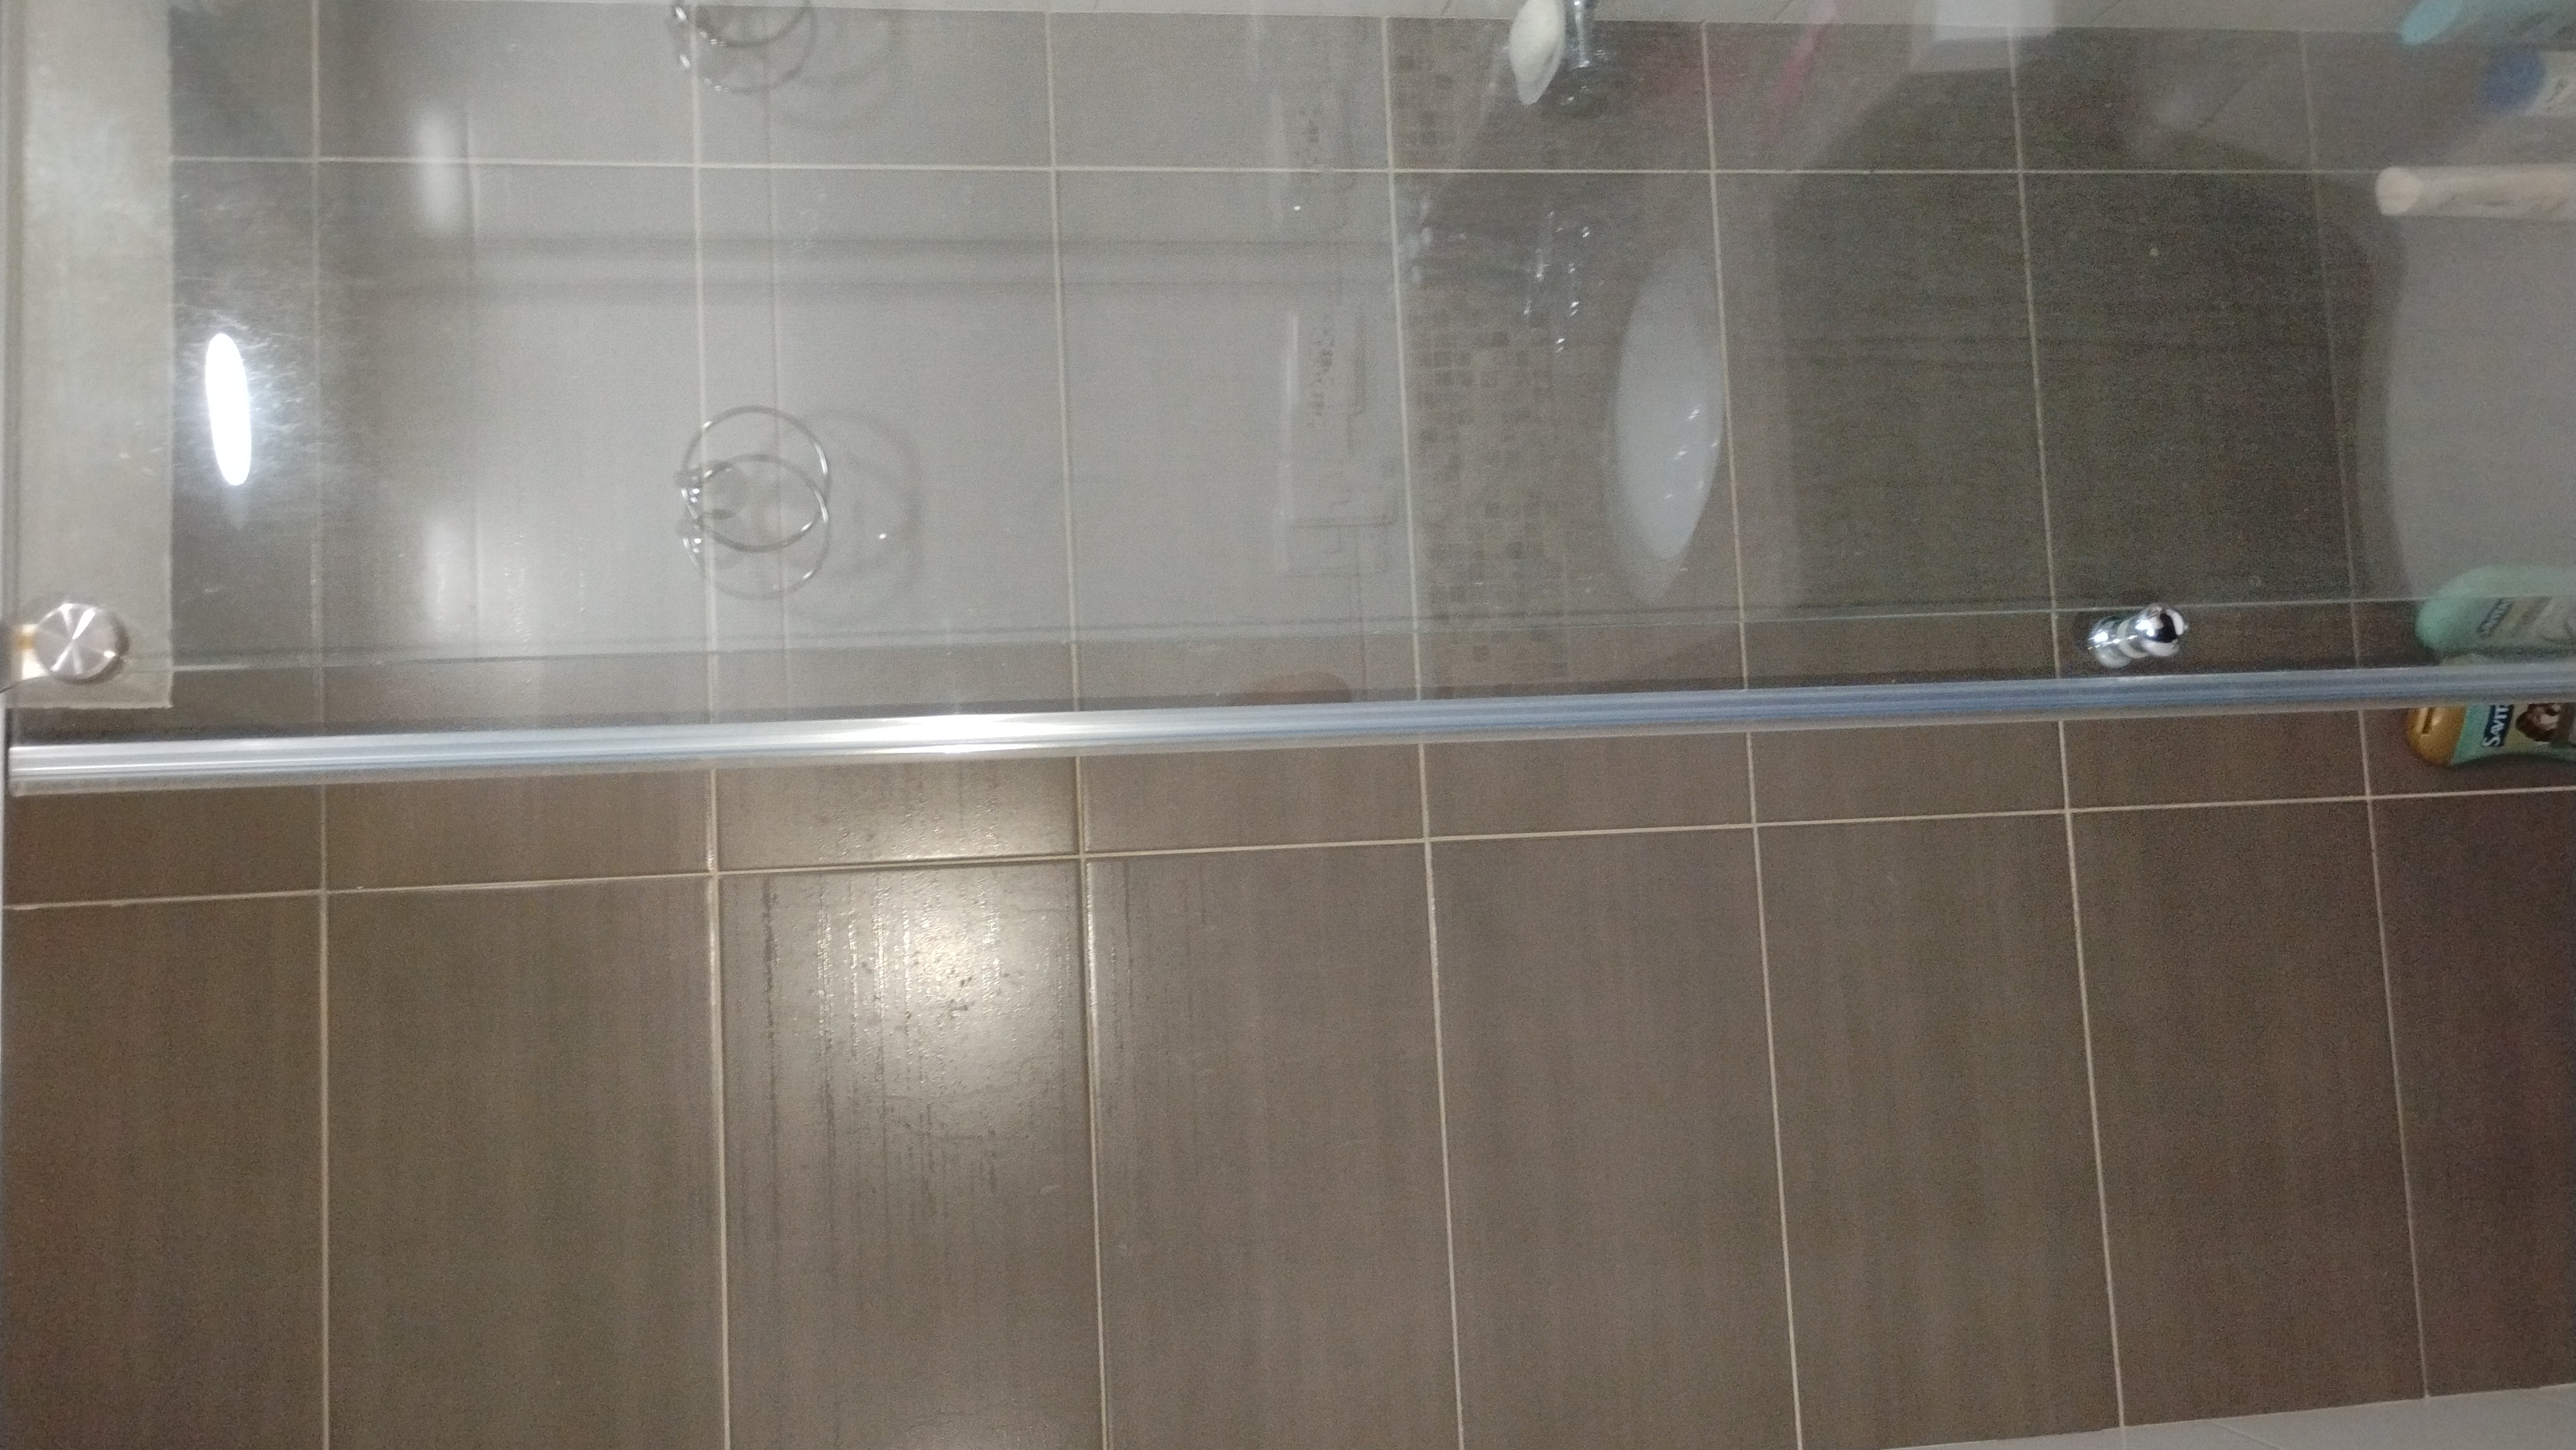
\includegraphics[width=\linewidth]{../img/IMG_20251109_151505065.jpg}\\[2pt]{\footnotesize\color{primary!60!black}Foto~74 -- 15:15:05}} \\[4pt]
\parbox{0.45\textwidth}{\centering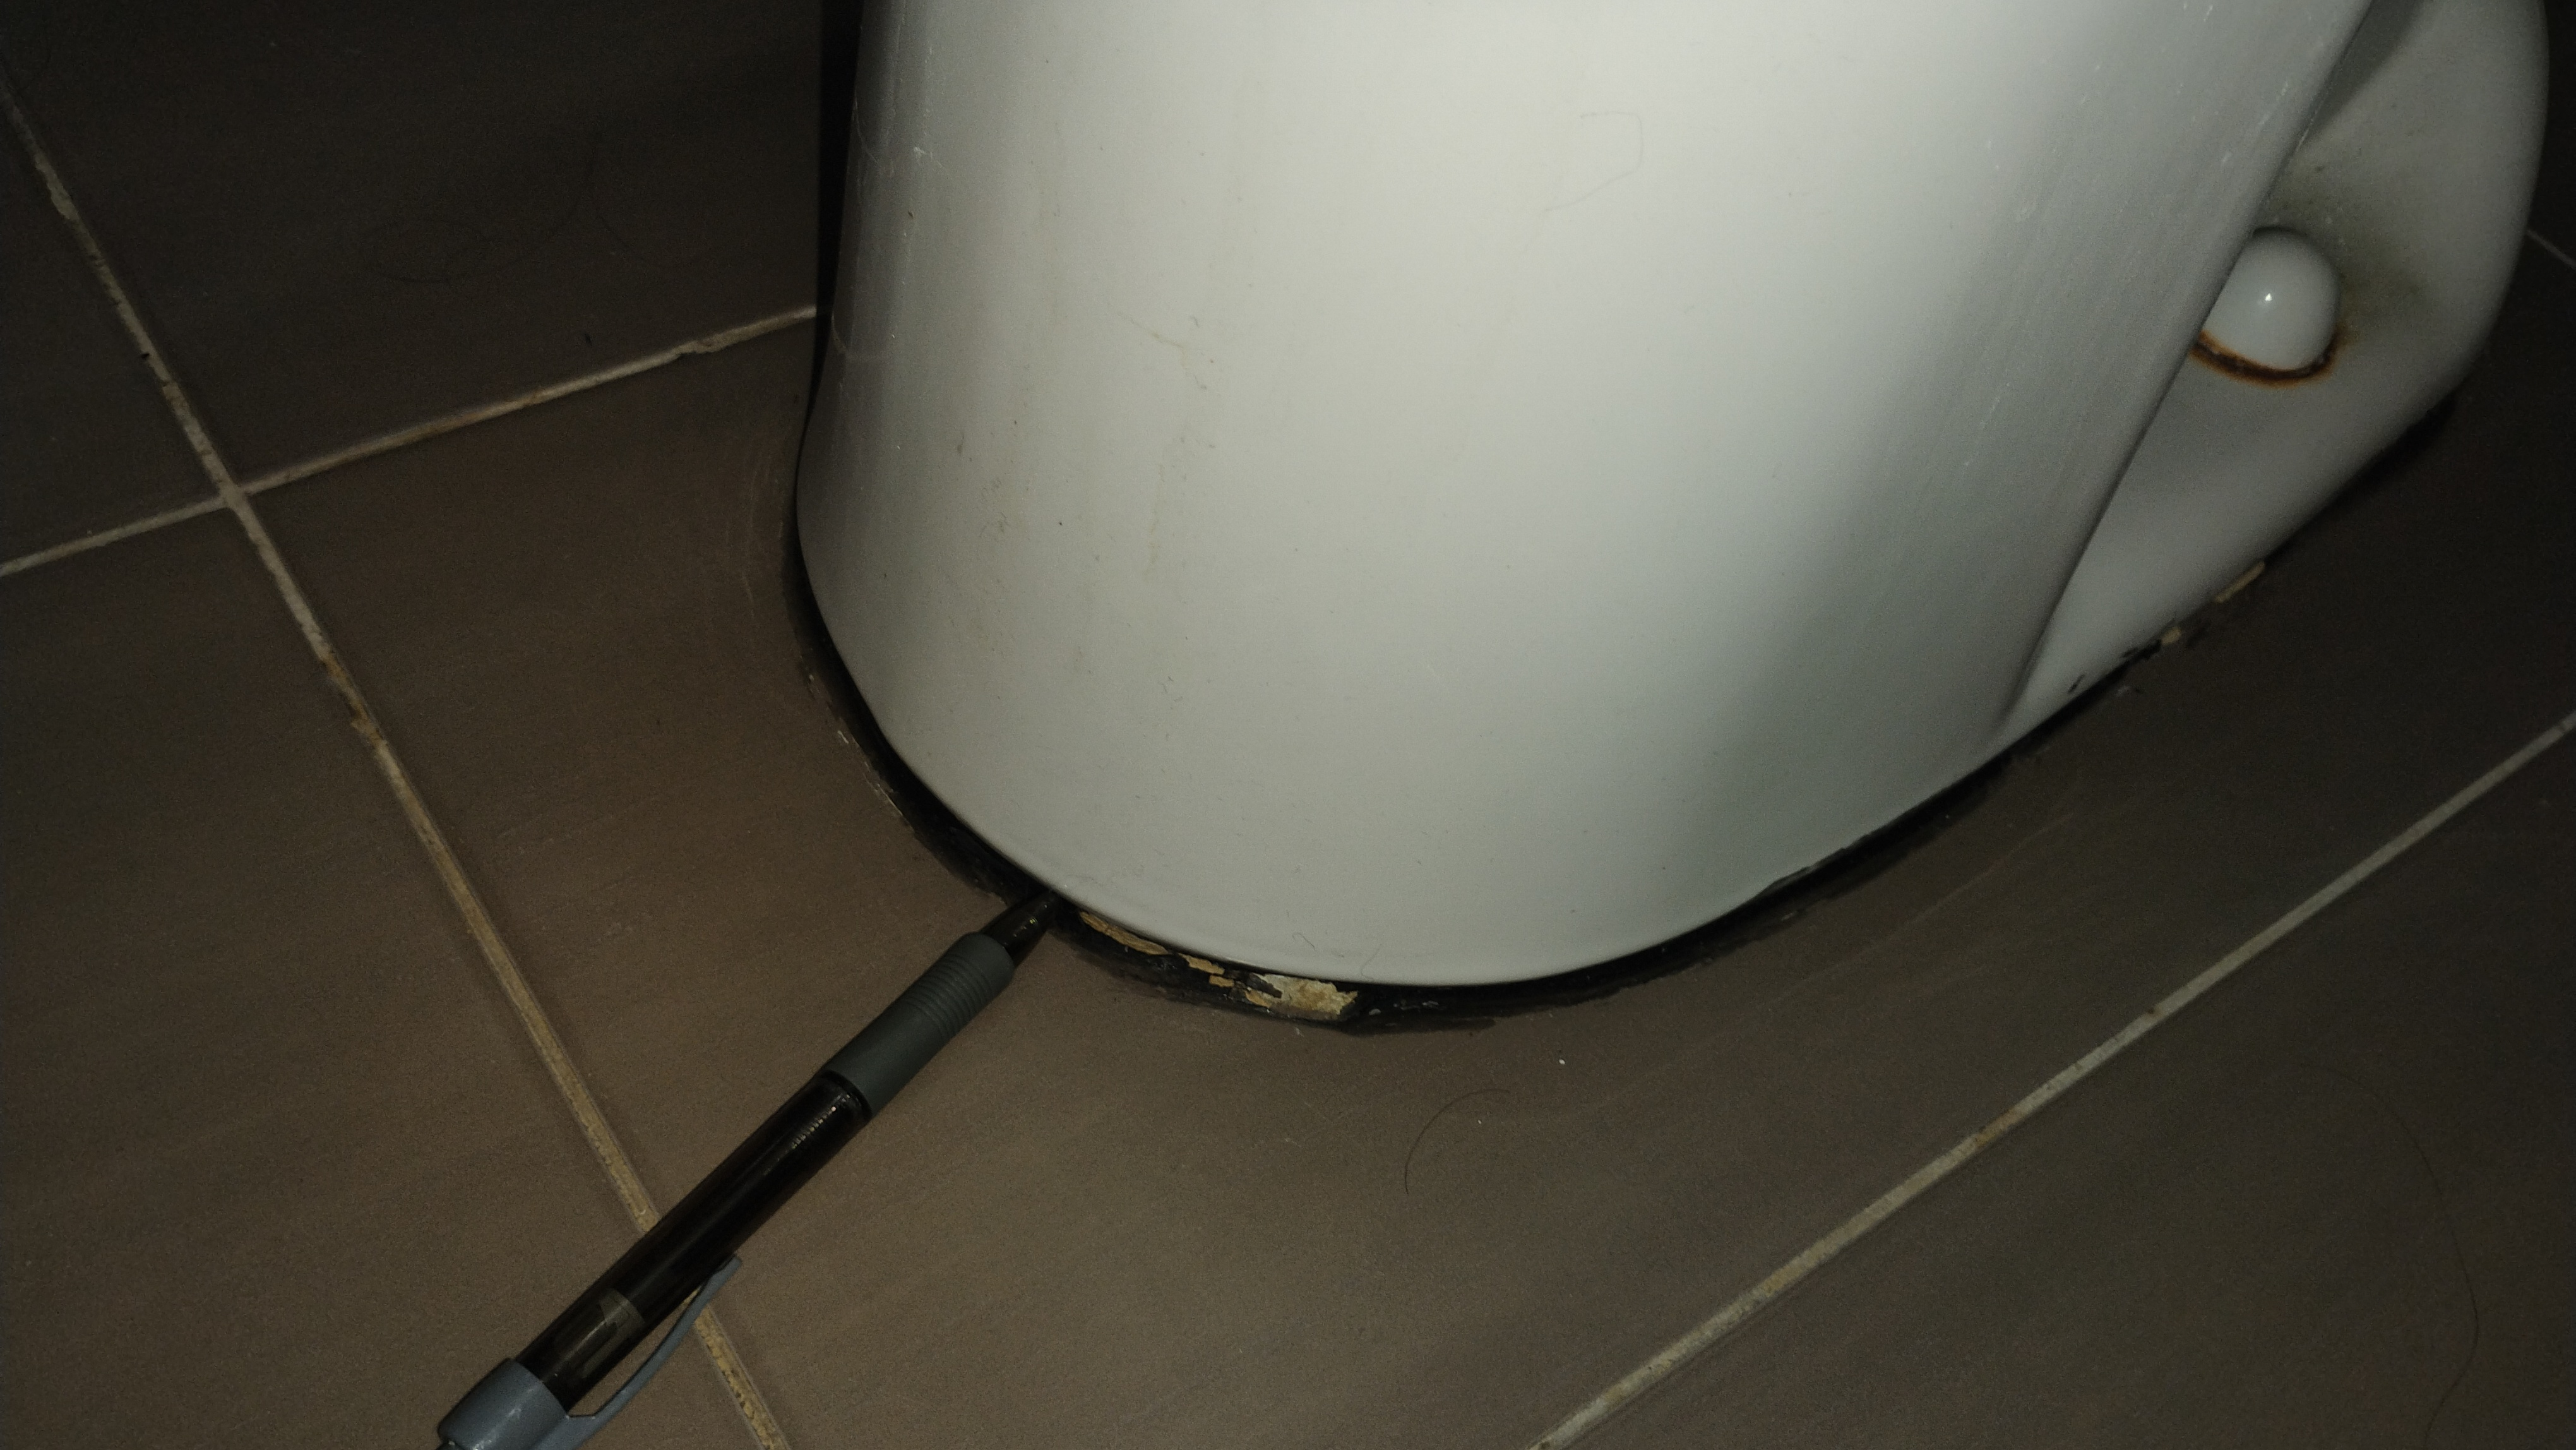
\includegraphics[width=\linewidth]{../img/IMG_20251109_151551470.jpg}\\[2pt]{\footnotesize\color{primary!60!black}Foto~75 -- 15:15:51}} & \parbox{0.45\textwidth}{\centering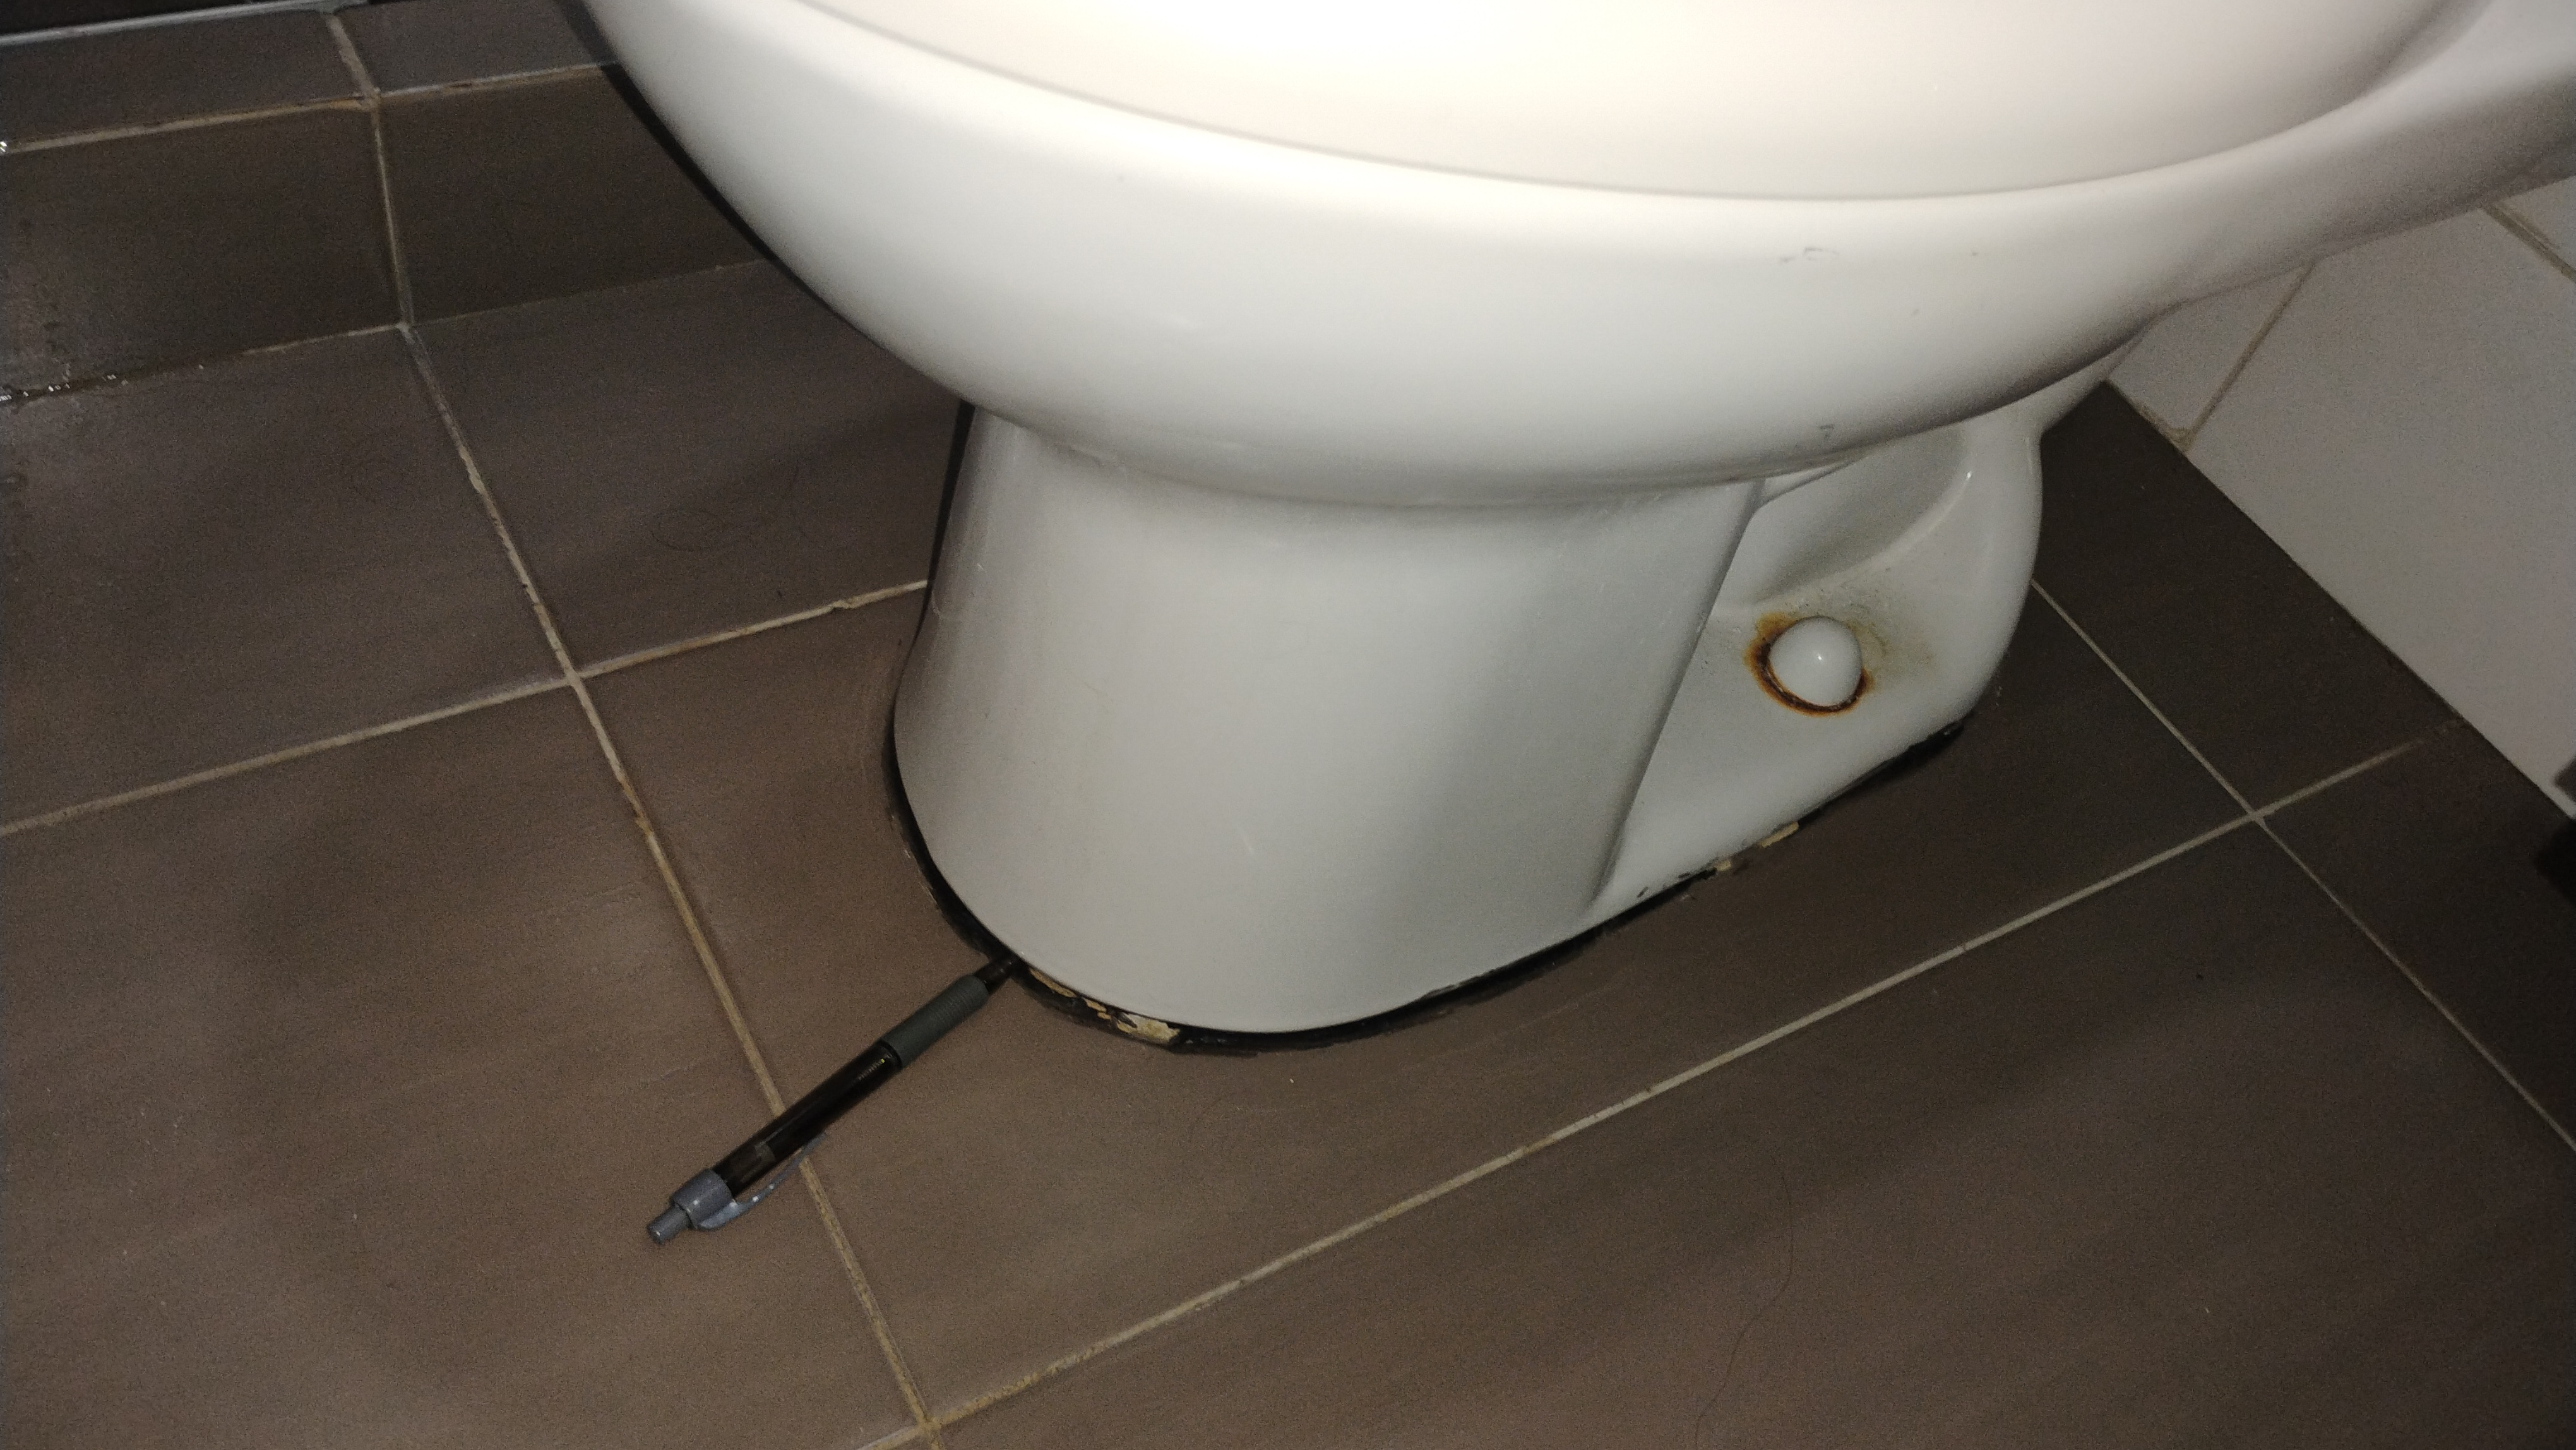
\includegraphics[width=\linewidth]{../img/IMG_20251109_151555467.jpg}\\[2pt]{\footnotesize\color{primary!60!black}Foto~76 -- 15:15:55}} \\[4pt]
\parbox{0.45\textwidth}{\centering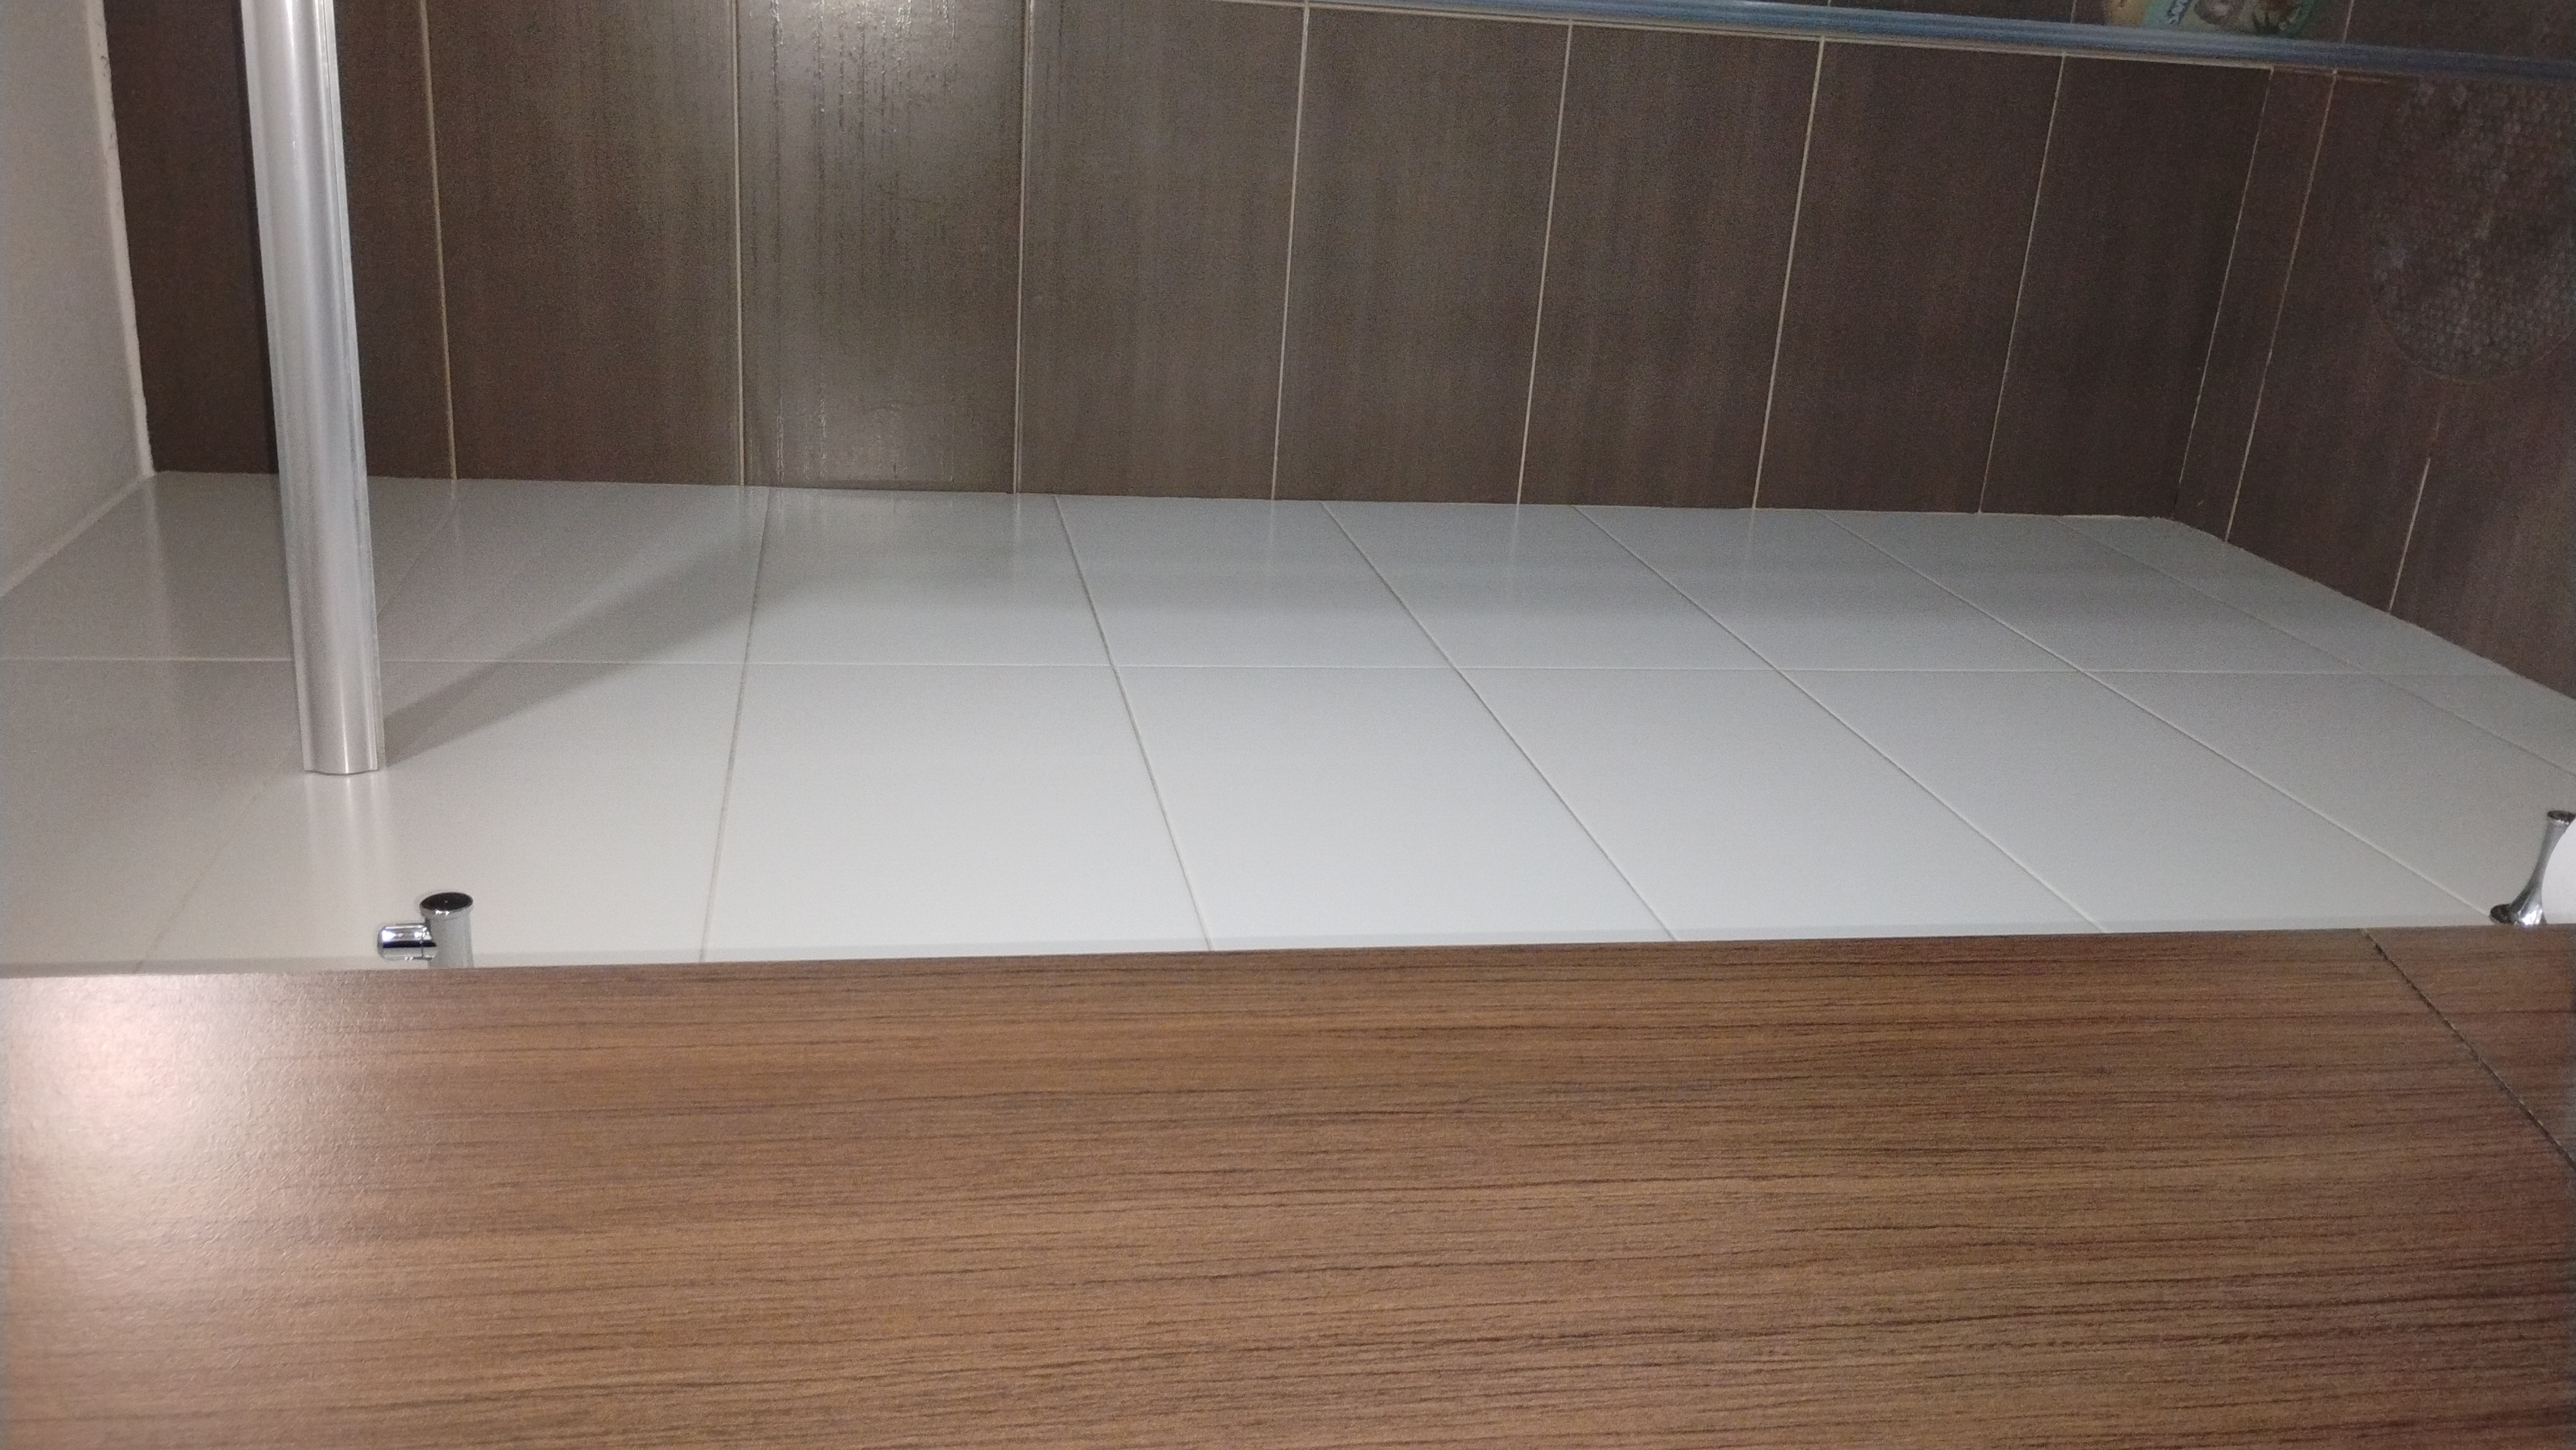
\includegraphics[width=\linewidth]{../img/IMG_20251109_151634335.jpg}\\[2pt]{\footnotesize\color{primary!60!black}Foto~77 -- 15:16:34}} & \parbox{0.45\textwidth}{\centering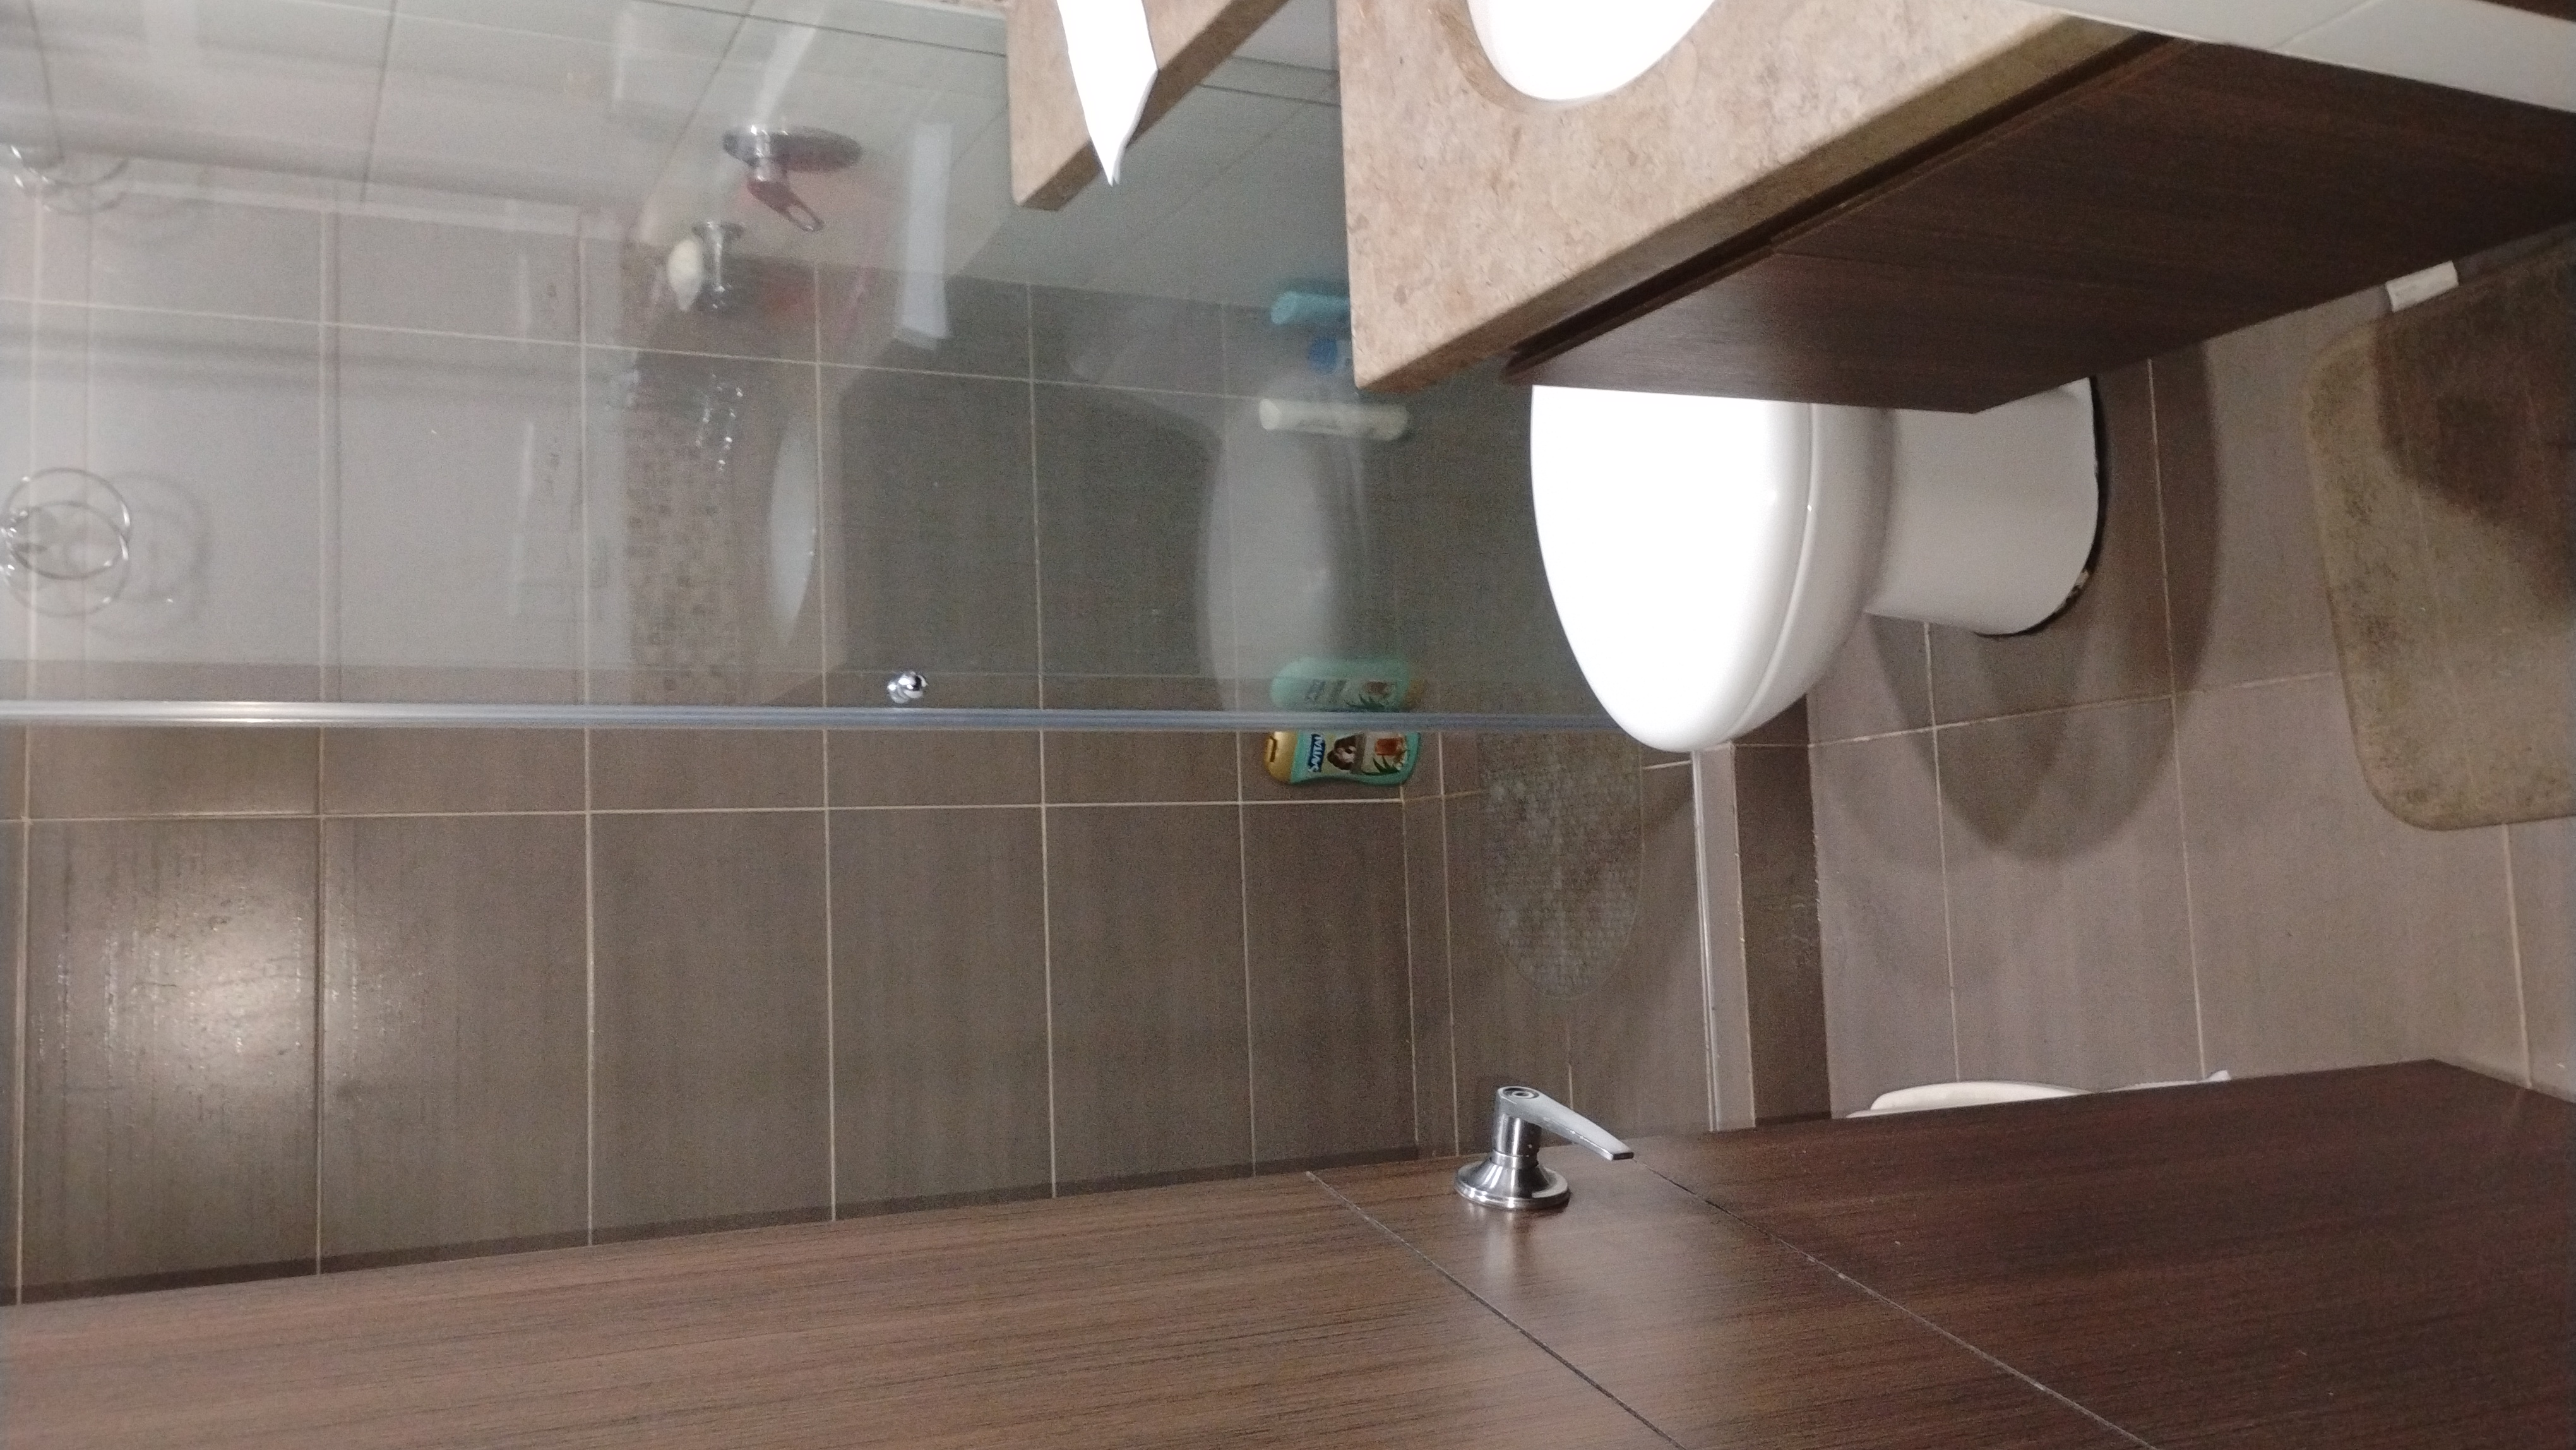
\includegraphics[width=\linewidth]{../img/IMG_20251109_151643114.jpg}\\[2pt]{\footnotesize\color{primary!60!black}Foto~78 -- 15:16:43}} \\[4pt]
\end{tabular}
\caption{Sanitario — Fisura en Porcelana y Válvula Mezcladora: Fotos 73 al 78.}\end{figure}
\newpage
\begin{figure}[H]
\centering
\begin{tabular}{cc}
\parbox{0.45\textwidth}{\centering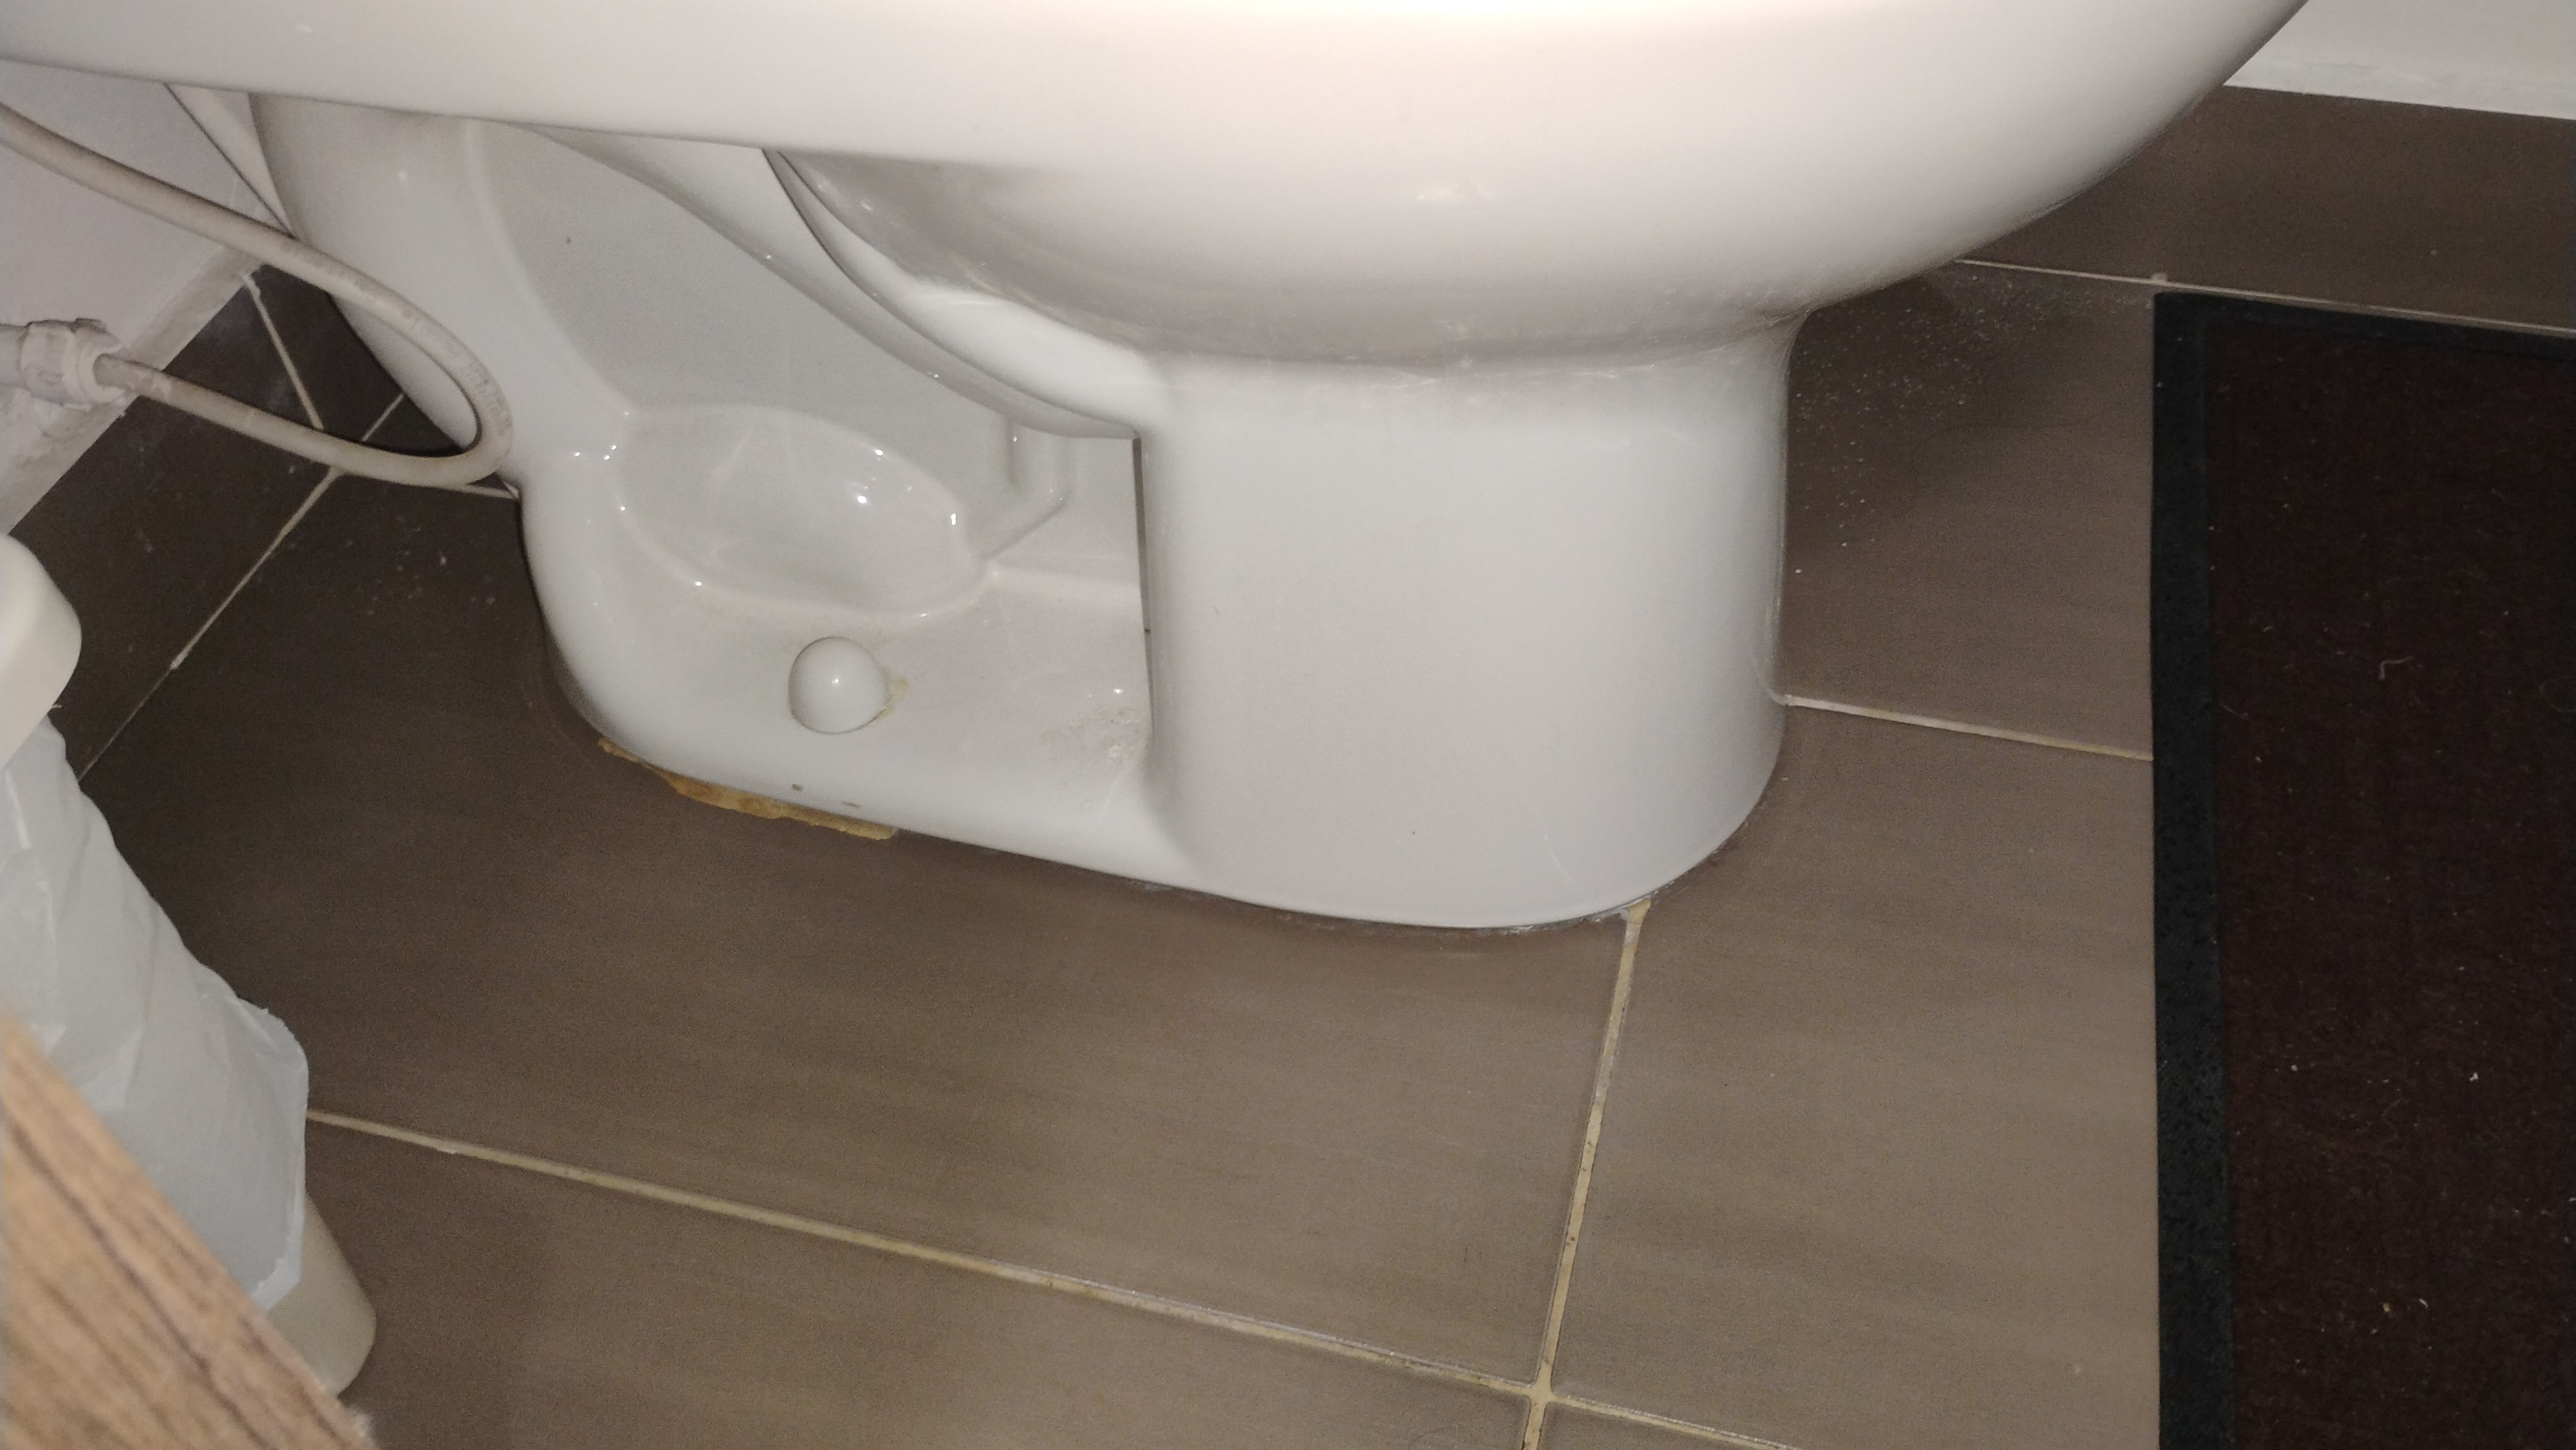
\includegraphics[width=\linewidth]{../img/IMG_20251109_151802456.jpg}\\[2pt]{\footnotesize\color{primary!60!black}Foto~79 -- 15:18:02}} & \\[4pt]
\end{tabular}
\caption{Cielorraso y Drenaje — Pañete y Deficiencia de Pendiente: Fotos 79 al 79.}\end{figure}
\newpage
\end{document}
